% main.tex —— 《局部 Langlands 对应的几何化：Berkeley 讲义》中译注本 主文件
% 底本：Peter Scholze 讲授，Tony Feng 记录，Geometrization of the Local Langlands
%       Correspondence（Berkeley 课程，2020-10-30 至 2021-02-12），148 页
%       印刷页 = PDF 页，偏移 0
% 编译：xelatex main ⇒ xelatex main ⇒ xelatex main
\documentclass[11pt,openany,oneside]{book}
% preamble.tex —— 《局部 Langlands 对应的几何化》中译注本 全局导言
% 编译：xelatex ×2（有索引时 xelatex → makeindex → xelatex ×2）
\usepackage[a4paper,margin=2.6cm,footskip=1.2cm]{geometry}
% 页锚放在页边：book 类默认 \marginparwidth=116pt，比 2.6cm 的页边距还宽，
% marginnote 会被排到纸外；这里把它压到页边距以内（编译自检见 _check*.log 的 Overfull）。
\setlength{\marginparwidth}{1.9cm}
\setlength{\marginparsep}{2pt}
\usepackage{ctex}
\usepackage{amsmath,amssymb,amsthm,mathtools}
\usepackage{mathrsfs,bbm}
\usepackage{stmaryrd}% \llbracket \rrbracket（原 s02/s03/s05/s08 各自 providecommand）
\usepackage{tikz}
\usepackage{tikz-cd}
\usetikzlibrary{arrows.meta,decorations.pathmorphing,calc}
\usepackage{xcolor}
\usepackage{enumitem}
\usepackage{booktabs,array,multirow}
\usepackage{graphicx}
\usepackage{marginnote}
\usepackage[unicode,bookmarksnumbered,bookmarksopen=true,hidelinks]{hyperref}
% 三级标题（1.4.1 这类）要编号：book 类默认 secnumdepth=2
\setcounter{secnumdepth}{3}
\usepackage{imakeidx}
\makeindex[intoc]

% ---------- 译者体例开关：\showyizhufalse 可一键隐藏全部译注 ----------
\newif\ifshowyizhu
\showyizhutrue

% ---------- 颜色 ----------
\definecolor{yizhuGray}{gray}{0.30}
\definecolor{srcBlue}{RGB}{20,70,140}

% ---------- 译注：\yizhu{内容}{来源} ----------
% 体例：以脚注形式排，楷体，来源用 [来源：…] 标注；无外部依据写 [译者按（无外部依据）]
\newcommand{\yizhu}[2]{%
  \ifshowyizhu
    \footnote{\textcolor{yizhuGray}{\kaishu #1}\quad{\scriptsize\textcolor{srcBlue}{[来源：#2]}}}%
  \fi}
\newcommand{\yizhuw}[1]{%
  \ifshowyizhu
    \footnote{\textcolor{yizhuGray}{\kaishu #1}\quad{\scriptsize\textcolor{srcBlue}{[译者按（无外部依据）]}}}%
  \fi}

% ---------- 原文页码锚点：\srcpage{7} ----------
% 1) 版式上用 marginnote（比 marginpar 稳：跨页段、定理环境、脚注附近都不易丢）；
% 2) 同时把页码写进 <jobname>.pagemarks，任何不可见的情况都能事后核查（工具见 tools/check_pagemarks.py）。
\newif\ifsrcmark
\srcmarktrue
\newwrite\srcpageout
\immediate\openout\srcpageout=\jobname.pagemarks
\newcommand{\srcpage}[1]{%
  \ifsrcmark\immediate\write\srcpageout{#1}\fi
  \phantomsection\label{srcpage:#1}%
  \marginnote{\raggedleft\scriptsize\textcolor{yizhuGray}{p.#1}}}
% 无 margin 的精简版（用于窄页/表格内）：\pgref{N}
\newcommand{\pgref}[1]{\textsuperscript{\scriptsize\textcolor{yizhuGray}{[p.#1]}}}
% 页界落在句子中间时用这个：行内小号上标，保证不会被排版吞掉
\newcommand{\srcpageinl}[1]{%
  \ifsrcmark\immediate\write\srcpageout{#1}\fi
  \phantomsection\label{srcpage:#1}%
  \textsuperscript{\tiny\textcolor{yizhuGray}{〔p.#1〕}}}


% ---------- 编号：章用罗马数字，节/定理沿用原文「I.6.3」式编号 ----------
% 本文是单篇综述：不用 chapter，节号从 1 起，与原文 1–9 一致
% 页眉：book 类默认 \sectionmark 为空（它靠 chapter 设 running head），
% 本文无 chapter，故自行设右页眉为「节号 节名」，\section* 处另加 \markright。
\renewcommand{\sectionmark}[1]{\markright{\thesection\quad #1}}
\renewcommand{\thesection}{\arabic{section}}
\renewcommand{\thesubsection}{\thesection.\arabic{subsection}}

% ---------- 定理环境（编号保持「章.节.序」） ----------
\theoremstyle{plain}
\newtheorem{theorem}{定理}[section]
\newtheorem{proposition}[theorem]{命题}
\newtheorem{lemma}[theorem]{引理}
\newtheorem{corollary}[theorem]{推论}
\theoremstyle{definition}
\newtheorem{definition}[theorem]{定义}
\newtheorem{example}[theorem]{例}
\newtheorem{construction}[theorem]{构造}
\newtheorem{question}[theorem]{问题}
\theoremstyle{remark}
\newtheorem{remark}[theorem]{注}
\newtheorem{conjecture}[theorem]{猜想}
% 作者自造的弱化断言 “Hope”（Hope 2.3、3.15、6.6），译作「期望」，与定理同计数器
\newtheorem{hope}[theorem]{期望}

% ---------- 常用记号 ----------
\newcommand{\FF}{\mathbb{F}}
\newcommand{\QQ}{\mathbb{Q}}
\newcommand{\ZZ}{\mathbb{Z}}
\newcommand{\RR}{\mathbb{R}}
\newcommand{\CC}{\mathbb{C}}
\newcommand{\PP}{\mathbb{P}}
\renewcommand{\AA}{\mathbb{A}}% 覆盖 Å
\newcommand{\GG}{\mathbb{G}}
\newcommand{\mm}{\mathfrak{m}}
\newcommand{\pp}{\mathfrak{p}}
\newcommand{\oo}{\mathcal{O}}
\newcommand{\Bun}{\mathrm{Bun}}
\newcommand{\Spa}{\mathrm{Spa}}
\newcommand{\SpaS}{\mathrm{Spa}}
\newcommand{\Div}{\mathrm{Div}}
\newcommand{\Gr}{\mathrm{Gr}}
\newcommand{\Hck}{\mathit{Hecke}}
\newcommand{\perf}{\mathrm{perf}}
\newcommand{\Adic}{\mathrm{Adic}}
\newcommand{\Crys}{\mathrm{Crys}}
\newcommand{\Isoc}{\mathrm{Isoc}}
\newcommand{\Vect}{\mathrm{Vect}}
\newcommand{\LocSys}{\mathrm{LocSys}}
\newcommand{\Rep}{\mathrm{Rep}}
\newcommand{\QCoh}{\mathrm{QCoh}}
\newcommand{\IndCoh}{\mathrm{IndCoh}}
\newcommand{\Dmod}{D\text{-}\mathrm{mod}}
\newcommand{\cD}{\mathcal{D}}
\newcommand{\cO}{\mathcal{O}}
\newcommand{\cF}{\mathcal{F}}
\newcommand{\cG}{\mathcal{G}}
\newcommand{\cH}{\mathcal{H}}
\newcommand{\cL}{\mathcal{L}}
\newcommand{\cM}{\mathcal{M}}
\newcommand{\cX}{\mathcal{X}}
\newcommand{\cY}{\mathcal{Y}}
\newcommand{\cZ}{\mathcal{Z}}
% 花体字母宏：\cA–\cZ 一次定义（译文中 \cE 等按需使用，避免逐字补漏）
\makeatletter
\@tfor\cletter:=ABCDEFGHIJKLMNOPQRSTUVWXYZ\do{%
  \expandafter\edef\csname c\cletter\endcsname{\noexpand\mathcal{\cletter}}}
\makeatother
\newcommand{\wt}[1]{\widetilde{#1}}
\newcommand{\ol}[1]{\overline{#1}}
\newcommand{\ul}[1]{\underline{#1}}
\DeclareMathOperator{\Spec}{Spec}
\DeclareMathOperator{\Aut}{Aut}
\DeclareMathOperator{\Hom}{Hom}
\DeclareMathOperator{\End}{End}
\DeclareMathOperator{\Ext}{Ext}
\DeclareMathOperator{\Tor}{Tor}
\DeclareMathOperator{\id}{id}
\DeclareMathOperator{\im}{im}
\DeclareMathOperator{\coker}{coker}
\DeclareMathOperator{\rk}{rk}
\DeclareMathOperator{\Pic}{Pic}
\DeclareMathOperator{\Lie}{Lie}
\DeclareMathOperator{\Sym}{Sym}
\DeclareMathOperator{\Ind}{Ind}
\DeclareMathOperator{\Res}{Res}
\DeclareMathOperator{\Gal}{Gal}
\DeclareMathOperator{\Weil}{Weil}
\DeclareMathOperator{\Frob}{Frob}
\DeclareMathOperator{\Sht}{Sht}
\DeclareMathOperator{\Art}{Art}
\DeclareMathOperator{\Proj}{Proj}
\DeclareMathOperator{\Spf}{Spf}
\DeclareMathOperator{\Isom}{Isom}
\DeclareMathOperator{\Tr}{Tr}
\DeclareMathOperator{\HN}{HN}
\DeclareMathOperator{\SpaO}{Spa}
\DeclareMathOperator{\Perf}{Perf}

% 交叉引用：\cref 风格
\newcommand{\thmref}[1]{定理~\ref{#1}}
\newcommand{\propref}[1]{命题~\ref{#1}}
\newcommand{\lemref}[1]{引理~\ref{#1}}
\newcommand{\defref}[1]{定义~\ref{#1}}
\newcommand{\remref}[1]{注~\ref{#1}}

% ========== SY02-41 追加宏（本讲义专用） ==========
\usepackage{mathrsfs}
\providecommand{\Fp}{\mathbb{F}_p}
\providecommand{\Fq}{\mathbb{F}_q}
\providecommand{\Fl}{\mathbb{F}_\ell}
\providecommand{\Qp}{\mathbb{Q}_p}
\providecommand{\Zp}{\mathbb{Z}_p}
\providecommand{\Ql}{\overline{\mathbb{Q}}_\ell}
\providecommand{\Zl}{\mathbb{Z}_\ell}
\providecommand{\breveE}{\breve{E}}
\providecommand{\Lam}{\Lambda}
\providecommand{\BdR}{B_{\mathrm{dR}}}
\providecommand{\Bcris}{B_{\mathrm{cris}}}
\providecommand{\Bst}{B_{\mathrm{st}}}
\providecommand{\BHT}{B_{\mathrm{HT}}}
\providecommand{\Ainf}{A_{\mathrm{inf}}}
\providecommand{\BunG}{\Bun_G}
\providecommand{\Perf}{\mathrm{Perf}}
\providecommand{\Fil}{\mathrm{Fil}}
\providecommand{\trdeg}{\operatorname{trdeg}}
\providecommand{\et}{\text{ét}}
\providecommand{\Et}{\mathrm{\acute{E}t}}
\providecommand{\diam}{{\diamondsuit}}
\providecommand{\cB}{\mathcal{B}}
\providecommand{\cC}{\mathcal{C}}
\providecommand{\cN}{\mathcal{N}}
\providecommand{\cP}{\mathcal{P}}
\providecommand{\cQ}{\mathcal{Q}}
\providecommand{\cS}{\mathcal{S}}
\providecommand{\cT}{\mathcal{T}}
\providecommand{\cU}{\mathcal{U}}
\providecommand{\cV}{\mathcal{V}}
\providecommand{\cW}{\mathcal{W}}
\providecommand{\cE}{\mathcal{E}}
\providecommand{\cK}{\mathcal{K}}
\providecommand{\cI}{\mathcal{I}}
\providecommand{\cJ}{\mathcal{J}}
\providecommand{\cA}{\mathcal{A}}
\providecommand{\Spd}{\mathrm{Spd}}
\providecommand{\Sm}{\mathrm{Sm}}
\providecommand{\Corr}{\mathrm{Corr}}
\providecommand{\Sht}{\mathrm{Sht}}
\providecommand{\BT}{\mathcal{BT}}
% 「警告」环境：原文 Warning n.m. 与定理同类，共用计数器
\theoremstyle{definition}
\newtheorem{warning}[theorem]{警告}
\newtheorem{notation}[theorem]{记号}
\newtheorem{fact}[theorem]{事实}
\newtheorem{exercise}[theorem]{练习}

% ---- 常用算子（补充，provide 语义避免重复定义） ----
\providecommand{\rank}{\operatorname{rank}}
\providecommand{\Spa}{\operatorname{Spa}}
\providecommand{\Isoc}{\operatorname{Isoc}}
\providecommand{\Rep}{\operatorname{Rep}}
\providecommand{\Perv}{\operatorname{Perv}}
\providecommand{\Spd}{\operatorname{Spd}}
% 底本用 99K 表示有理映射
\providecommand{\dashto}{\dashrightarrow}

% ---- 常用域符号（译手偶用单字母写法，统一 provide 出来） ----
\providecommand{\Q}{\mathbb{Q}}
\providecommand{\Z}{\mathbb{Z}}
\providecommand{\C}{\mathbb{C}}
\providecommand{\R}{\mathbb{R}}
\providecommand{\F}{\mathbb{F}}
\providecommand{\A}{\mathbb{A}}
\providecommand{\G}{\mathbb{G}}
\providecommand{\P}{\mathbb{P}}

% ================================================================
% figs-batch1.tex —— 讲义手绘示意图的 TikZ 重绘（第 1 批，共 9 幅）
% 覆盖 p.10, p.11（2 幅）, p.24, p.43（2 幅）, p.44, p.45, p.50。
% 只含图体（tikzpicture），不含 figure 环境与 caption，不引用外部图片。
%
% 命名：\figP<页>-<序>。LaTeX 控制序列名不能含数字，直接写 \newcommand{\figP010}
% 会报错（控制序列被截断），故一律用 \csname 定义；正文调用写
%   \figP{010}、\figP{011-1}、\figP{043-2} …（文件末尾的 \figP 转发），
% 或直接写 \csname figP010\endcsname。
% ================================================================

% p.10：闭环单位圆盘 $\mathbb B_C$ 内的环带 $\mathbb A(\epsilon,r)$（灰色阴影），圆心穿孔标 ×
\expandafter\newcommand\csname figP010\endcsname{%
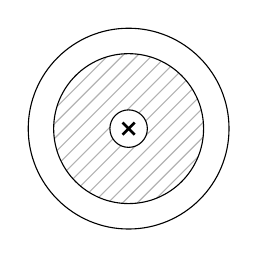
\begin{tikzpicture}[scale=0.85]
  \begin{scope}
    \clip (0,0) circle (1.12);
    \foreach \y in {-1.9,-1.68,...,1.9}
      \draw[gray!60] (-1.6,\y-1.6) -- (1.6,\y+1.6);
  \end{scope}
  \fill[white] (0,0) circle (0.28);
  \draw (0,0) circle (1.5);
  \draw (0,0) circle (1.12);
  \draw (0,0) circle (0.28);
  \draw[line width=0.9pt] (-0.09,-0.09)--(0.09,0.09) (0.09,-0.09)--(-0.09,0.09);
\end{tikzpicture}}

% p.11：Frobenius $\phi_C$ 在 $\mathbb D_C^\times$ 上的自由、真不连续作用：每点沿轨道向外移动
\expandafter\newcommand\csname figP011-1\endcsname{%
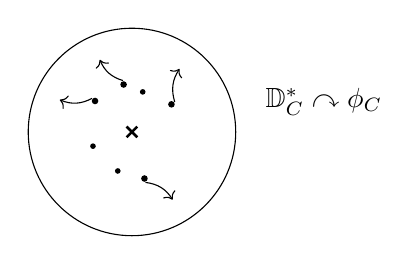
\begin{tikzpicture}[scale=0.85]
  \draw (0,0) circle (1.55);
  \draw[line width=0.9pt] (-0.08,-0.08)--(0.08,0.08) (0.08,-0.08)--(-0.08,0.08);
  \foreach \a/\da in {140/16, 100/14, 35/18, 285/16} {
    \fill (\a:0.72) circle (1.4pt);
    \draw[->] (\a:0.78) to[bend left=25] (\a+\da:1.18);
  }
  \foreach \a in {75, 200, 250} \fill (\a:0.62) circle (1.2pt);
  \node[right] at (1.85,0.45) {$\mathbb D_C^*\curvearrowright\phi_C$};
\end{tikzpicture}}

% p.11：环带 $\mathbb A(r,r^{1/q})$ 上 Frobenius 把内边界点送往外边界点；下方为商 $X_{C,E}$（环面）
\expandafter\newcommand\csname figP011-2\endcsname{%
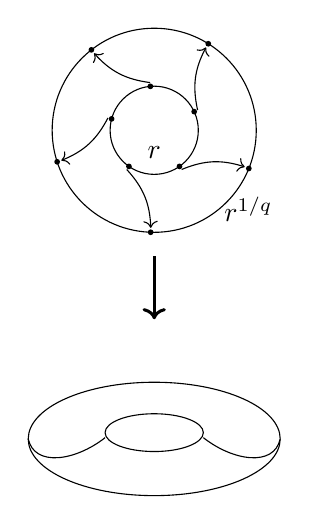
\begin{tikzpicture}[scale=0.8]
  \draw (0,0) circle (1.62);
  \draw (0,0) circle (0.7);
  \foreach \a in {25, 95, 165, 235, 305} {
    \fill (\a:0.7) circle (1.3pt);
    \fill (\a+33:1.62) circle (1.3pt);
    \draw[->] (\a:0.76) to[bend left=20] (\a+33:1.55);
  }
  \node at (270:0.35) {$r$};
  \node at (320:1.95) {$r^{1/q}$};
  \draw[->, line width=1.1pt] (0,-2.0) -- (0,-3.0);
  \begin{scope}[shift={(0,-4.9)}]
    \draw (0,0) ellipse (2.0 and 0.9);
    \draw (0,0.10) ellipse (0.78 and 0.30);
    \draw (-2.0,0) .. controls (-1.9,-0.45) and (-1.25,-0.35) .. (-0.78,0.02);
    \draw (2.0,0) .. controls (1.9,-0.45) and (1.25,-0.35) .. (0.78,0.02);
  \end{scope}
\end{tikzpicture}}

% p.24：Warning 5.6 的图——分歧映射的曲线（源曲线蛇形覆于底曲线之上，分歧点处打孔）
\expandafter\newcommand\csname figP024\endcsname{%
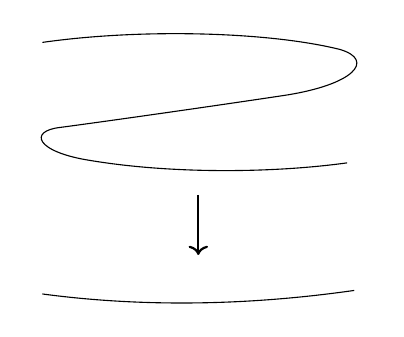
\begin{tikzpicture}[scale=0.9]
  \draw (-2.2,2.45) .. controls (-0.8,2.65) and (1.0,2.6) .. (2.0,2.35)
        .. controls (2.5,2.2) and (2.2,1.85) .. (1.2,1.7)
        .. controls (0.2,1.55) and (-1.2,1.35) .. (-1.95,1.25)
        .. controls (-2.4,1.2) and (-2.3,0.9) .. (-1.5,0.78)
        .. controls (-0.4,0.6) and (1.0,0.6) .. (2.1,0.75);
  \draw[->, line width=0.8pt] (0,0.3) -- (0,-0.55);
  \draw (-2.2,-1.1) .. controls (-0.7,-1.3) and (0.8,-1.25) .. (2.2,-1.05);
\end{tikzpicture}}

% p.43：$\mathcal M_{\mathrm{ell},\mathbf C_p,\infty}$ 经 Hodge–Tate 周期映射到 $\mathbf P^1_{\mathbb Q_p}$；
%        左侧叠层曲线上的两列红盘是超奇异约化的圆盘，下方椭圆上的红盘同此
\expandafter\newcommand\csname figP043-1\endcsname{%
\begin{tikzpicture}[scale=0.8]
  \draw (-3.4,3.45) .. controls (-1.9,3.6) and (-0.2,3.55) .. (0.5,3.35);
  \draw (-3.4,3.0) .. controls (-1.8,3.2) and (-0.1,3.1) .. (0.55,2.95)
        .. controls (0.95,2.85) and (0.8,2.65) .. (0.15,2.65);
  \draw (-3.4,2.55) .. controls (-1.8,2.75) and (0.0,2.6) .. (0.55,2.5)
        .. controls (0.95,2.4) and (0.8,2.2) .. (0.15,2.2);
  \draw (-3.4,2.1) .. controls (-1.7,2.3) and (0.1,2.2) .. (0.6,2.05);
  \draw (-3.4,1.65) .. controls (-1.9,1.8) and (-0.4,1.75) .. (0.4,1.65);
  \foreach \x in {-2.2,-0.9}
    \foreach \y in {3.6,3.26,2.92,2.58,2.24,1.9,1.56,1.22} {
      \fill[red!75] (\x,\y) ellipse (0.27 and 0.16);
      \draw[red!55!black] (\x,\y) ellipse (0.27 and 0.16);
    }
  \draw[->] (0.7,3.45) -- (1.5,3.65);
  \node[right] at (1.55,3.65) {$\mathbf P^1_{\mathbb Q_p}$};
  \node at (3.0,2.4) {$\mathcal M_{\mathrm{ell},\mathbf C_p,\infty}$};
  \draw[->] (3.0,2.0) -- (3.0,1.45);
  \node at (3.0,1.15) {$\mathcal M_{\mathrm{ell},\mathbf C_p}$};
  \draw (-1.6,-0.8) ellipse (1.9 and 0.66);
  \foreach \x/\y in {-2.45/0.2,-1.55/0.42,-0.6/0.15} {
    \draw[red!60!black] (\x,-0.14) -- (\x,\y-0.15);
    \fill[red!75] (\x,\y) ellipse (0.25 and 0.16);
    \draw[red!55!black] (\x,\y) ellipse (0.25 and 0.16);
  }
  \node[red!70!black] at (-1.6,-2.05) {\small 超奇异约化的圆盘};
\end{tikzpicture}}

% p.43：超奇异圆盘的原像（左上不规则区域）经 Hodge–Tate 映射落入
%        $\mathbf P^1_{\mathbf C_p}\setminus\mathbf P^1(\mathbf Q_p)=\Omega^2$；左下椭圆为约化圆盘
\expandafter\newcommand\csname figP043-2\endcsname{%
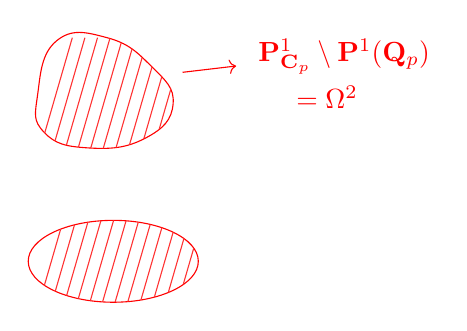
\begin{tikzpicture}[scale=0.8, color=red]
  \draw plot[smooth cycle, tension=0.8] coordinates
    {(-3.3,1.4) (-3.0,2.25) (-2.2,2.3) (-1.5,1.85) (-1.15,1.25) (-1.6,0.7) (-2.5,0.55) (-3.2,0.8)};
  \begin{scope}
    \clip plot[smooth cycle, tension=0.8] coordinates
      {(-3.3,1.4) (-3.0,2.25) (-2.2,2.3) (-1.5,1.85) (-1.15,1.25) (-1.6,0.7) (-2.5,0.55) (-3.2,0.8)};
    \foreach \x in {-3.3,-3.1,...,-1.3} \draw[red!80] (\x,0.4) -- ++(0.55,1.9);
  \end{scope}
  \draw[->] (-1.0,1.75) -- (-0.15,1.85);
  \node[right] at (0.05,2.0) {$\mathbf P^1_{\mathbf C_p}\setminus\mathbf P^1(\mathbf Q_p)$};
  \node[right] at (0.65,1.35) {$=\Omega^2$};
  \draw (-2.1,-1.25) ellipse (1.35 and 0.65);
  \begin{scope}
    \clip (-2.1,-1.25) ellipse (1.35 and 0.65);
    \foreach \x in {-3.3,-3.1,...,-0.9} \draw[red!80] (\x,-2.0) -- ++(0.55,1.9);
  \end{scope}
\end{tikzpicture}}

% p.44：向量丛 $\mathcal E$ 的 Newton 多边形；横轴为 length（秩方向），各级斜率 $\lambda$
%        的重数 $n_\lambda(\xi)$ 决定折点，终点坐标为 $(\mathrm{rank},\mathrm{degree})$
\expandafter\newcommand\csname figP044\endcsname{%
\begin{tikzpicture}[scale=0.85]
  \draw (-1.2,0) -- (6.2,0);
  \draw (0,-1.9) -- (0,4.0);
  \draw[red, line width=1.1pt] (0,0) -- (2.6,-1.35) -- (4.6,-0.95) -- (5.7,2.85);
  \node[right] at (5.75,2.85) {\small $(\text{秩},\text{次数})$};
  \node at (-0.55,-2.1) {\small 长度};
  \node[right] at (1.0,-2.05) {\small $(\lambda\mapsto n_\lambda(\xi))$};
  \draw[->] (-0.2,-1.8) .. controls (0.05,-1.55) and (0.3,-1.3) .. (0.5,-1.02);
\end{tikzpicture}}

% p.45：例 9.3 的两条 Newton 多边形——$\mathcal O(-\frac12)$（斜率 $-1/2$，端点为 $(2,-1)$）
%        与 $\mathcal O\oplus\mathcal O(-1)$（折点 $(1,-1)$、$(2,-1)$）
\expandafter\newcommand\csname figP045\endcsname{%
\begin{tikzpicture}[scale=0.8]
  \draw (-1.3,4.9) -- (4.2,4.9);
  \draw (0,3.5) -- (0,7.1);
  \draw[red, line width=1.1pt] (0,4.9) -- (2.0,3.9);
  \fill (2.0,3.9) circle (1.3pt);
  \node[above left] at (0,6.95) {$\mathcal O(-\tfrac12)$};
  \node[below left] at (0,4.85) {\scriptsize $(0,0)$};
  \node[below right] at (2.0,3.85) {\scriptsize $(2,-1)$};
  \draw (-1.3,0.2) -- (4.2,0.2);
  \draw (0,-1.3) -- (0,2.3);
  \draw[red, line width=1.1pt] (0,0.2) -- (1.3,-1.1) -- (3.0,-1.1);
  \fill (1.3,-1.1) circle (1.3pt);
  \fill (3.0,-1.1) circle (1.3pt);
  \node[above left] at (0,2.15) {$\mathcal O\oplus\mathcal O(-1)$};
  \node[below left] at (0,0.15) {\scriptsize $(0,0)$};
  \node[below] at (1.3,-1.15) {\scriptsize $(1,-1)$};
  \node[below] at (3.0,-1.15) {\scriptsize $(2,-1)$};
\end{tikzpicture}}

% p.50：宽度为 $n$ 的 Newton 多边形——折点坐标为整数（break points integral），终点为 $(n,d)$
\expandafter\newcommand\csname figP050\endcsname{%
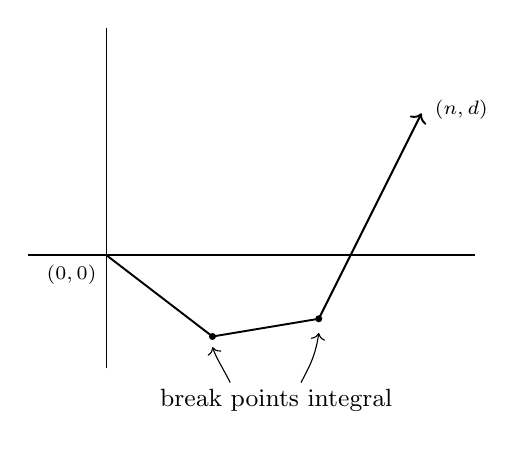
\begin{tikzpicture}[scale=0.9]
  \draw (-1.1,0) -- (5.2,0);
  \draw (0,-1.6) -- (0,3.2);
  \draw[->, line width=0.7pt] (0,0) -- (1.5,-1.15) -- (3.0,-0.9) -- (4.45,2.0);
  \fill (1.5,-1.15) circle (1.4pt);
  \fill (3.0,-0.9) circle (1.4pt);
  \node[below left] at (0,0) {\scriptsize $(0,0)$};
  \node[right] at (4.5,2.05) {\scriptsize $(n,d)$};
  \node at (2.4,-2.05) {\small break points integral};
  \draw[->] (1.75,-1.8) .. controls (1.65,-1.6) and (1.55,-1.45) .. (1.5,-1.3);
  \draw[->] (2.75,-1.8) .. controls (2.85,-1.6) and (2.95,-1.45) .. (3.0,-1.1);
\end{tikzpicture}}

% 转发宏：正文写 \figP{010}、\figP{011-1} 等（用 \providecommand，避免多批文件重复定义）
\providecommand{\figP}[1]{\csname figP#1\endcsname}

% ================================================================
% figs-batch2.tex —— 第 2 批手绘示意图的 TikZ 重绘（15 幅图体）
% 覆盖 p.51（2 幅）、p.52、p.63、p.65、p.77、p.85、p.97（2 幅）、
%      p.106、p.107、p.120、p.121（2 幅）、p.122。
% 只含图体：不含 figure 环境与 caption，不引用外部图片，不写
% \usepackage、\usetikzlibrary（假定已装载 arrows.meta, calc,
% decorations.pathmorphing, patterns）。
% 命名 figP<页>[A|B]。控制序列名不能含数字，故用 \csname 定义；
% 正文写 \figP{051A}、\figP{121B}（文件末有转发宏）。
% p.121 的 X^+ / X^- 原文并排为同一幅图，也可分开使用。
% ================================================================

% p.51：$|\Bun_1|=|\mathrm{Pic}|\cong\mathbb Z$ 离散，点是 $\mathcal O(i)$（例 10.6）
\expandafter\newcommand\csname figP051A\endcsname{%
\begin{tikzpicture}[scale=0.9]
  \node[left] at (-0.3,0) {$|\Bun_1|$};
  \foreach \y/\l in {2.0/{$\mathcal O(2)$},1.0/{$\mathcal O(1)$},0/{$0$},
                     -1.0/{$\mathcal O(-1)$},-2.0/{$\mathcal O(-2)$}}{%
    \fill (0.6,\y) circle (1.5pt);
    \node[right] at (0.8,\y) {\small \l};}
  \node at (0.6,2.75) {$\vdots$};
  \node at (0.6,-2.75) {$\vdots$};
\end{tikzpicture}}

% p.51：$|\Bun_2|$ 按次数 $d$ 分层，每层唯一半稳定点 $\mathcal O(d/2)$；
% 红色波浪箭头是特化，向右越来越特殊（例 10.7，$\otimes\mathcal O(1)$ 使其 2-周期）
\expandafter\newcommand\csname figP051B\endcsname{%
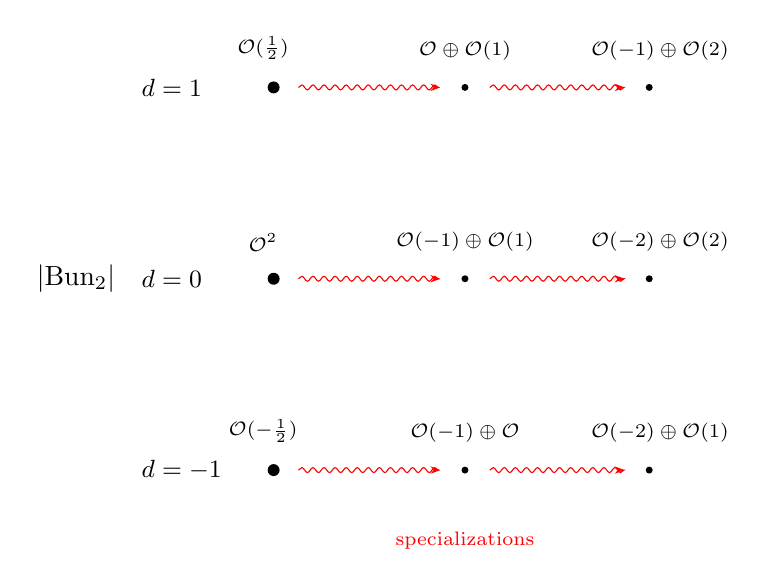
\begin{tikzpicture}[scale=0.9,
  sp/.style={red,decorate,decoration={snake,amplitude=0.9pt,segment length=4pt}}]
  \node[left] at (-0.5,0.2) {$|\Bun_2|$};
  \foreach \y/\d in {2.9/{$d=1$},0.2/{$d=0$},-2.5/{$d=-1$}}
    \node[right] at (-0.4,\y) {\small \d};
  \foreach \y in {2.9,0.2,-2.5}{%
    \fill (1.6,\y) circle (2.4pt);
    \fill (4.3,\y) circle (1.4pt);
    \fill (6.9,\y) circle (1.4pt);
    \draw[sp,-{Stealth[length=3.5pt]}] (1.95,\y) -- (3.95,\y);
    \draw[sp,-{Stealth[length=3.5pt]}] (4.65,\y) -- (6.55,\y);}
  \node[above] at (1.45,3.15) {\scriptsize $\mathcal O(\tfrac12)$};
  \node[above] at (4.3,3.15) {\scriptsize $\mathcal O\oplus\mathcal O(1)$};
  \node[above] at (7.05,3.15) {\scriptsize $\mathcal O(-1)\oplus\mathcal O(2)$};
  \node[above] at (1.45,0.45) {\scriptsize $\mathcal O^2$};
  \node[above] at (4.3,0.45) {\scriptsize $\mathcal O(-1)\oplus\mathcal O(1)$};
  \node[above] at (7.05,0.45) {\scriptsize $\mathcal O(-2)\oplus\mathcal O(2)$};
  \node[above] at (1.45,-2.25) {\scriptsize $\mathcal O(-\tfrac12)$};
  \node[above] at (4.3,-2.25) {\scriptsize $\mathcal O(-1)\oplus\mathcal O$};
  \node[above] at (7.05,-2.25) {\scriptsize $\mathcal O(-2)\oplus\mathcal O(1)$};
  \node[red] at (4.3,-3.5) {\scriptsize specializations};
\end{tikzpicture}}

% p.52：$|\Bun_3|$ 的 $d=0$ 层开头——$\mathcal O^3$ 特化到两个半稳定点，
% 二者又同样特化到 $\mathcal O(-1)\oplus\mathcal O\oplus\mathcal O(1)$（例 10.8）
\expandafter\newcommand\csname figP052\endcsname{%
\begin{tikzpicture}[scale=0.9,
  sp/.style={red,decorate,decoration={snake,amplitude=0.9pt,segment length=4pt}}]
  \node[left] at (-1.0,0.6) {$|\Bun_3|$};
  \node[left] at (-1.0,-0.2) {\small $d=0$};
  \fill (0,0) circle (2.4pt);
  \node[below left] at (-0.15,-0.2) {\small $\mathcal O^3$};
  \fill (2.6,2.0) circle (1.5pt);
  \fill (2.6,-2.0) circle (1.5pt);
  \fill (5.2,0.35) circle (1.5pt);
  \node[above] at (2.6,2.25) {\scriptsize $\mathcal O(-\tfrac12)\oplus\mathcal O(1)$};
  \node[below] at (2.6,-2.25) {\scriptsize $\mathcal O(-1)\oplus\mathcal O(\tfrac12)$};
  \node[below right] at (5.05,0.0) {\scriptsize $\mathcal O(-1)\oplus\mathcal O\oplus\mathcal O(1)$};
  \draw[sp,-{Stealth[length=3.5pt]}] (0.35,0.3) -- (2.25,1.78);
  \draw[sp,-{Stealth[length=3.5pt]}] (0.35,-0.3) -- (2.25,-1.78);
  \draw[sp,-{Stealth[length=3.5pt]}] (2.95,1.8) -- (4.9,0.6);
  \draw[sp,-{Stealth[length=3.5pt]}] (2.95,-1.8) -- (4.9,-0.6);
  \node at (7.6,2.05) {$\cdots$};
  \node at (7.6,-2.05) {$\cdots$};
\end{tikzpicture}}

% p.63：$R$ 的“单参数形变”。底部是 $\Spa R^\flat$，四条竖线是 $\xi$-方向纤维，
% 横穿的黑曲线 $\xi_R=\Spa W_{\mathcal O_E}(R^{\flat\circ})\setminus V([\![\varpi]\!])$
% 上的红带子是 $B^+_{dR}$ 部分（§12.3）
\expandafter\newcommand\csname figP063\endcsname{%
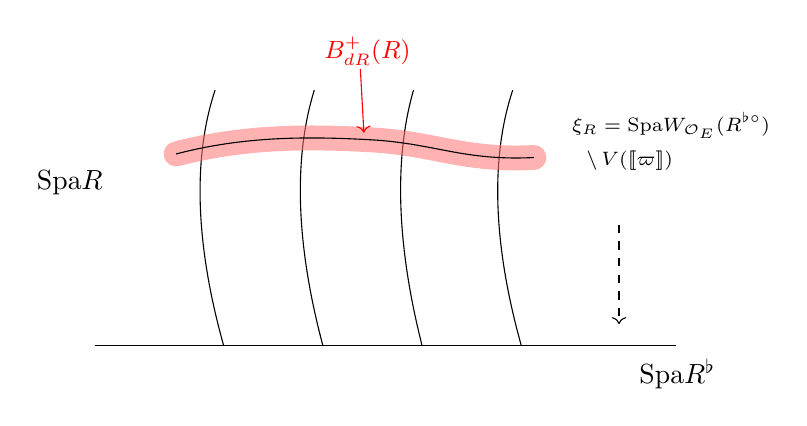
\begin{tikzpicture}[scale=0.9]
  \draw (-0.6,0) -- (7.6,0);
  \foreach \x/\d in {1.1/-0.30,2.5/-0.28,3.9/-0.26,5.3/-0.30}
    \draw (\x,3.6) .. controls (\x+\d,2.7) and (\x+\d,1.5) .. (\x+0.12,0);
  \draw[red!55,line width=9pt,opacity=0.55,line cap=round]
        (0.55,2.7) .. controls (1.5,2.95) and (2.4,2.95) .. (3.3,2.9)
        .. controls (4.2,2.85) and (4.6,2.6) .. (5.6,2.65);
  \draw (0.55,2.7) .. controls (1.5,2.95) and (2.4,2.95) .. (3.3,2.9)
        .. controls (4.2,2.85) and (4.6,2.6) .. (5.6,2.65);
  \node[red] at (3.25,4.15) {\small $B^+_{dR}(R)$};
  \draw[->,red] (3.15,3.9) -- (3.2,3.0);
  \node at (-0.95,2.3) {$\Spa R$};
  \node[anchor=west] at (6.0,3.1) {\scriptsize $\xi_R=\Spa W_{\mathcal O_E}(R^{\flat\circ})$};
  \node[anchor=west] at (6.2,2.6) {\scriptsize $\setminus\,V([\![\varpi]\!])$};
  \draw[->,dashed] (6.8,1.7) -- (6.8,0.3);
  \node[below right] at (6.95,-0.05) {$\Spa R^\flat$};
\end{tikzpicture}}

% p.65：代数曲线 $X^{\mathrm{alg}}_{S^\flat}$ 上的点 $s$ 对应 $\Spa B^+_{dR}(R)$，
% 即 $\mathcal E'|_{X_s}$ 的局部模型（定理 12.25 证明）
\expandafter\newcommand\csname figP065\endcsname{%
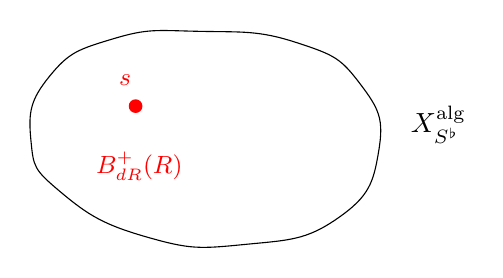
\begin{tikzpicture}[scale=0.95]
  \draw plot[smooth cycle,tension=0.85] coordinates
    {(-2.45,0.1) (-2.2,0.95) (-1.35,1.45) (-0.2,1.55) (1.1,1.4) (1.95,0.85)
     (2.2,-0.05) (1.65,-0.95) (0.4,-1.3) (-0.9,-1.2) (-2.05,-0.6)};
  \fill[red] (-1.05,0.55) circle (2.6pt);
  \node[red,above left] at (-0.98,0.7) {\small $s$};
  \node[red] at (-1.0,-0.25) {\small $B^+_{dR}(R)$};
  \node[right] at (2.5,0.3) {$X^{\mathrm{alg}}_{S^\flat}$};
\end{tikzpicture}}

% p.77：$\mathbb B_C$（左）、$\mathbb P^1_C$（右）、典范紧化
% $\overline{\mathbb B}^{\,/C}_C$（下）；紧化只多加一个“半径 $1$ 再加无穷小”的
% rank 2 点（例 14.12）。虚线弧表示树在无穷处继续
\expandafter\newcommand\csname figP077\endcsname{%
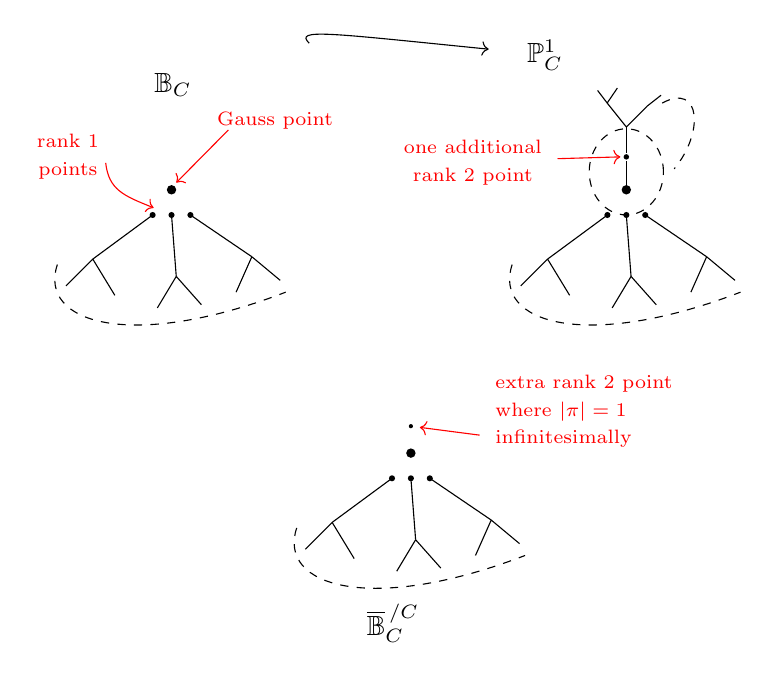
\begin{tikzpicture}[scale=0.76,
  tree/.pic={\fill (0,0) circle (1.7pt);
    \foreach \a in {-0.24,0,0.24} \fill (\a,-0.32) circle (1.1pt);
    \draw (-0.24,-0.32) -- (-1.00,-0.88) (0,-0.32) -- (0.06,-1.10)
          (0.24,-0.32) -- (1.02,-0.85);
    \draw (-1.00,-0.88) -- (-1.34,-1.22) (-1.00,-0.88) -- (-0.72,-1.34);
    \draw (0.06,-1.10) -- (-0.18,-1.50) (0.06,-1.10) -- (0.38,-1.46);
    \draw (1.02,-0.85) -- (0.82,-1.30) (1.02,-0.85) -- (1.38,-1.15);
    \draw[dashed] (-1.45,-0.95) .. controls (-1.70,-1.70) and (-0.50,-2.05) .. (1.45,-1.30);}]
  \pic at (0,0) {tree};
  \node[anchor=west] at (-0.45,1.75) {$\mathbb B_C$};
  \node[red,anchor=west] at (0.60,1.15) {\scriptsize Gauss point};
  \draw[->,red] (0.95,1.00) -- (0.08,0.12);
  \node[red,align=center,anchor=east] at (-1.05,0.55)
    {\scriptsize rank 1\\[-2pt]\scriptsize points};
  \draw[->,red] (-1.10,0.45) .. controls (-1.05,0.0) and (-0.80,-0.10) .. (-0.30,-0.30);
  \draw[->] (2.3,2.45) .. controls (2.05,2.70) and (2.6,2.62) .. (5.3,2.35);
  \pic at (7.6,0) {tree};
  \draw (7.6,0) -- (7.6,0.48);
  \fill (7.6,0.55) circle (1.3pt);
  \draw (7.6,0.62) -- (7.6,1.05);
  \draw (7.6,1.05) -- (7.28,1.45) (7.6,1.05) -- (7.95,1.40);
  \draw (7.28,1.45) -- (7.12,1.66) (7.28,1.45) -- (7.45,1.70);
  \draw (7.95,1.40) -- (8.18,1.58);
  \draw[dashed] (7.6,0.30) ellipse (0.62 and 0.72);
  \draw[dashed] (8.20,1.45) .. controls (8.85,1.80) and (8.90,0.95) .. (8.40,0.35);
  \node[red,align=center,anchor=east] at (6.35,0.45)
    {\scriptsize one additional\\[-2pt]\scriptsize rank 2 point};
  \draw[->,red] (6.45,0.52) -- (7.50,0.55);
  \node[anchor=east] at (6.70,2.25) {$\mathbb P^1_C$};
  \pic at (4.0,-4.4) {tree};
  \fill (4.0,-3.95) circle (1.0pt);
  \draw[->,red] (5.15,-4.10) -- (4.15,-3.97);
  \node[red,align=left,anchor=west] at (5.25,-3.70)
    {\scriptsize extra rank 2 point\\[-2pt]\scriptsize where $|\pi|=1$\\[-2pt]\scriptsize infinitesimally};
  \node[anchor=north] at (3.70,-6.75) {$\overline{\mathbb B}^{\,/C}_C$};
\end{tikzpicture}}

% p.85：$|\Bun_G|$ 一条连通分支内的特化图景：每层的点都特化到更特殊的点，
% 一路到底即半稳定层 $\Bun^{ss}_G$（推论 16.2：连通分支 = 某半稳定层的闭包）
\expandafter\newcommand\csname figP085\endcsname{%
\begin{tikzpicture}[scale=1.1,
  sp/.style={red,decorate,decoration={snake,amplitude=0.9pt,segment length=4pt}}]
  \foreach \x in {1.0,2.0} \fill ( \x,3.7) circle (2.2pt);
  \fill (3.6,3.7) circle (2.6pt);
  \fill (5.2,3.7) circle (4.2pt);
  \draw[sp,-{Stealth[length=3.5pt]}] (4.8,3.7) -- (4.0,3.7);
  \draw[sp,-{Stealth[length=3.5pt]}] (3.3,3.8) -- (2.4,4.0);
  \draw[sp,-{Stealth[length=3.5pt]}] (3.3,3.6) -- (2.4,3.4);
  \draw[sp,-{Stealth[length=3.5pt]}] (1.8,4.0) -- (1.2,4.05);
  \draw[sp,-{Stealth[length=3.5pt]}] (1.8,3.4) -- (1.2,3.35);
  \fill (5.2,1.1) circle (4.2pt);
  \foreach \y in {1.75,1.1,0.45} \fill (3.6,\y) circle (2.6pt);
  \foreach \y in {1.95,1.1,0.25} \fill (2.0,\y) circle (2.6pt);
  \foreach \y in {1.75,1.1,0.45}
    \draw[sp,-{Stealth[length=3.5pt]}] (4.8,\y) -- (4.0,\y);
  \foreach \y/\z in {1.75/1.95,1.1/1.1,0.45/0.25}
    \draw[sp,-{Stealth[length=3.5pt]}] (3.3,\y) -- (2.4,\z);
  \foreach \x in {3.2,3.55,3.9} \fill[red] (\x,-1.2) circle (2.2pt);
  \fill (5.2,-1.2) circle (4.2pt);
  \foreach \y in {-1.9,-2.3,-2.7} \fill (5.2,\y) circle (1.6pt);
  \draw (4.5,-3.15) .. controls (4.75,-3.0) and (5.0,-3.3) .. (5.3,-3.1)
        .. controls (5.5,-2.95) and (5.7,-3.15) .. (5.8,-3.3);
  \node at (5.2,-3.85) {$\Bun^{ss}_G$};
  \draw[->] (5.9,3.7) -- (7.2,3.7);
  \node at (0.55,3.7) {$\cdots$};
  \node at (0.55,1.1) {$\cdots$};
\end{tikzpicture}}

% p.97：$|X_{\bar x}|$ 与 $|S_{\bar s}|$ 都是全序点链；$|S_{\bar t}|\subset|S_{\bar s}|$
% 是其中的子链（椭圆圈出），竖箭头是 $X_{\bar x}\to S_{\bar s}$（注 18.18）
\expandafter\newcommand\csname figP097A\endcsname{%
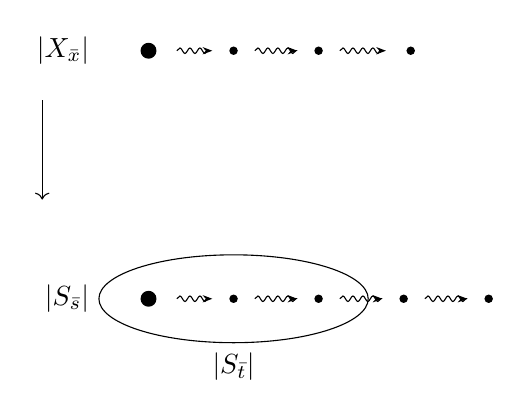
\begin{tikzpicture}[scale=0.9,
  sq/.style={decorate,decoration={snake,amplitude=1.0pt,segment length=3.6pt}}]
  \node[left] at (1.5,3.2) {$|X_{\bar x}|$};
  \fill (2.2,3.2) circle (3.2pt);
  \foreach \x in {3.4,4.6,5.9} \fill (\x,3.2) circle (1.7pt);
  \draw[sq,-{Stealth[length=3.5pt]}] (2.6,3.2) -- (3.1,3.2);
  \draw[sq,-{Stealth[length=3.5pt]}] (3.7,3.2) -- (4.3,3.2);
  \draw[sq,-{Stealth[length=3.5pt]}] (4.9,3.2) -- (5.55,3.2);
  \draw[->] (0.7,2.5) -- (0.7,1.1);
  \node[left] at (1.5,-0.3) {$|S_{\bar s}|$};
  \fill (2.2,-0.3) circle (3.2pt);
  \foreach \x in {3.4,4.6,5.8,7.0} \fill (\x,-0.3) circle (1.7pt);
  \draw[sq,-{Stealth[length=3.5pt]}] (2.6,-0.3) -- (3.1,-0.3);
  \draw[sq,-{Stealth[length=3.5pt]}] (3.7,-0.3) -- (4.3,-0.3);
  \draw[sq,-{Stealth[length=3.5pt]}] (4.9,-0.3) -- (5.5,-0.3);
  \draw[sq,-{Stealth[length=3.5pt]}] (6.1,-0.3) -- (6.7,-0.3);
  \draw (3.4,-0.3) ellipse (1.9 and 0.62);
  \node at (3.4,-1.25) {$|S_{\bar t}|$};
\end{tikzpicture}}

% p.97：过收敛（overconvergent）。把树上的点 $x$ 放大：黑块是点本身，
% 三个红点是它周围的 rank 1 点，四条短线是各个方向（注 18.18 之后的直观图）
\expandafter\newcommand\csname figP097B\endcsname{%
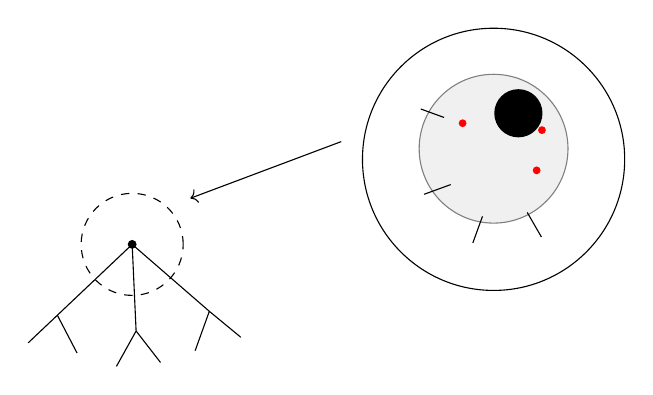
\begin{tikzpicture}[scale=0.9,
  tree/.pic={\fill (0,0) circle (1.6pt);
    \draw (0,0) -- (-0.95,-0.9) (0,0) -- (0.05,-1.1) (0,0) -- (0.98,-0.85);
    \draw (-0.95,-0.9) -- (-1.32,-1.25) (-0.95,-0.9) -- (-0.70,-1.38);
    \draw (0.05,-1.1) -- (-0.20,-1.55) (0.05,-1.1) -- (0.36,-1.50);
    \draw (0.98,-0.85) -- (0.80,-1.35) (0.98,-0.85) -- (1.38,-1.18);}]
  \pic at (0.8,-0.1) {tree};
  \draw[dashed] (0.8,-0.1) circle (0.72);
  \draw[->] (3.75,1.35) -- (1.62,0.55);
  \draw (5.9,1.1) circle (1.85);
  \fill[gray!12] (5.9,1.25) circle (1.05);
  \draw[gray] (5.9,1.25) circle (1.05);
  \fill (6.25,1.75) circle (0.34);
  \foreach \a in {150,20,-35} \fill[red] ($(6.0,1.3)+(\a:0.62)$) circle (0.055);
  \draw ($(6.0,1.0)+(200:0.75)$) -- ($(6.0,1.0)+(200:1.15)$);
  \draw ($(6.0,1.0)+(250:0.75)$) -- ($(6.0,1.0)+(250:1.15)$);
  \draw ($(6.0,1.0)+(300:0.75)$) -- ($(6.0,1.0)+(300:1.15)$);
  \draw ($(6.0,1.4)+(160:0.85)$) -- ($(6.0,1.4)+(160:1.20)$);
\end{tikzpicture}}

% p.106：$\tilde M_b\cong\mathcal{BC}(\mathcal O(-1)[1])$ 是开单位圆盘；中心是
% $t=0$，右上边界圈出被挖去的点 $*$——它在 $|t|=1$ 处（警告 19.16）
\expandafter\newcommand\csname figP106\endcsname{%
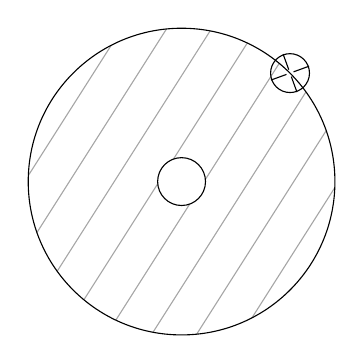
\begin{tikzpicture}[scale=0.95]
  \begin{scope}
    \clip (0,0) circle (2.05);
    \foreach \t in {-2.8,-2.2,...,2.8} \draw[gray!70] (\t-1.3,-2.2) -- (\t+1.5,2.2);
  \end{scope}
  \draw (0,0) circle (2.05);
  \fill[white] (0,0) circle (0.32);
  \draw (0,0) circle (0.32);
  \draw (1.45,1.45) circle (0.26);
  \foreach \a in {20,110,200,290}
    \draw (1.45,1.45) ++(\a:0.05) -- ++(\a:0.22);
\end{tikzpicture}}

% p.107：直观图——$M$ 带自由的 $\mathbb R$-作用（水平流线），$M/\mathbb R$ 紧
% （椭圆是截面），流的两个端点是“源”和“汇”（定理 19.19 的证明）
\expandafter\newcommand\csname figP107\endcsname{%
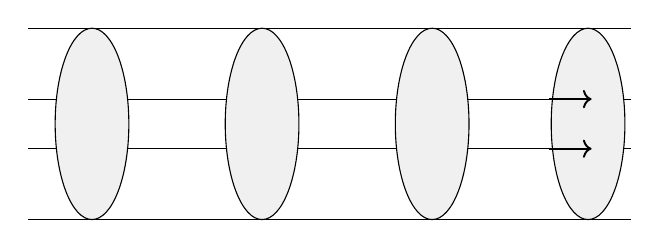
\begin{tikzpicture}[scale=0.9]
  \draw (0,2.85) -- (8.5,2.85);
  \draw (0,1.85) -- (8.5,1.85);
  \draw (0,1.15) -- (8.5,1.15);
  \draw (0,0.15) -- (8.5,0.15);
  \foreach \x in {0.9,3.3,5.7,7.9} \fill[gray!12] (\x,1.5) ellipse (0.52 and 1.35);
  \foreach \x in {0.9,3.3,5.7,7.9} \draw (\x,1.5) ellipse (0.52 and 1.35);
  \draw[->,line width=0.7pt] (7.35,1.85) -- (7.95,1.85);
  \draw[->,line width=0.7pt] (7.35,1.15) -- (7.95,1.15);
\end{tikzpicture}}

% p.120：树上的点及其放大（残余圆盘）。黑块是 rank 2 点、红点是 rank 1 点，
% 短线表示各方向——点的维数正是由此读出的（§22.3，例 22.15）
\expandafter\newcommand\csname figP120\endcsname{%
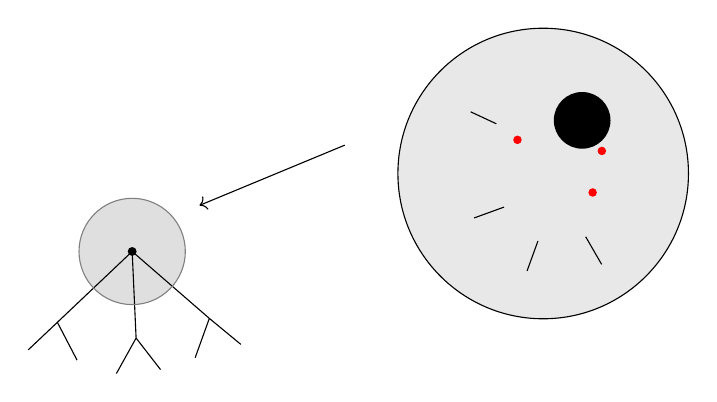
\begin{tikzpicture}[scale=0.9,
  tree/.pic={\fill (0,0) circle (1.6pt);
    \draw (0,0) -- (-0.95,-0.9) (0,0) -- (0.05,-1.1) (0,0) -- (0.98,-0.85);
    \draw (-0.95,-0.9) -- (-1.32,-1.25) (-0.95,-0.9) -- (-0.70,-1.38);
    \draw (0.05,-1.1) -- (-0.20,-1.55) (0.05,-1.1) -- (0.36,-1.50);
    \draw (0.98,-0.85) -- (0.80,-1.35) (0.98,-0.85) -- (1.38,-1.18);}]
  \fill[gray!25] (0.6,0.1) circle (0.75);
  \pic at (0.6,0.1) {tree};
  \draw[gray] (0.6,0.1) circle (0.75);
  \draw[->] (3.6,1.6) -- (1.55,0.75);
  \fill[gray!18] (6.4,1.2) circle (2.05);
  \draw (6.4,1.2) circle (2.05);
  \fill (6.95,1.95) circle (0.40);
  \foreach \a in {150,15,-40} \fill[red] ($(6.6,1.35)+(\a:0.65)$) circle (0.06);
  \draw ($(6.6,1.0)+(200:0.8)$) -- ($(6.6,1.0)+(200:1.25)$);
  \draw ($(6.6,1.0)+(250:0.8)$) -- ($(6.6,1.0)+(250:1.25)$);
  \draw ($(6.6,1.0)+(300:0.8)$) -- ($(6.6,1.0)+(300:1.25)$);
  \draw ($(6.6,1.5)+(155:0.95)$) -- ($(6.6,1.5)+(155:1.35)$);
\end{tikzpicture}}

% p.121：$\mathbb P^1$ 上的标准 $\mathbb G_m$-作用，分层 $X^+=\mathbb A^1\sqcup\{\infty\}$：
% 蓝色流线都汇向 $0$，赤道前半实线、后半虚线（例 22.17）
\expandafter\newcommand\csname figP121A\endcsname{%
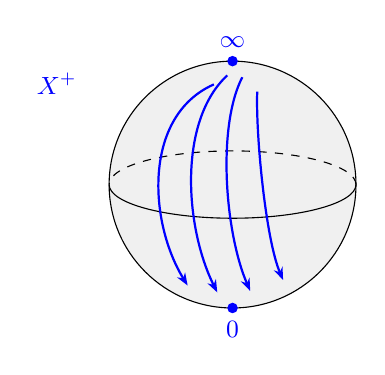
\begin{tikzpicture}[scale=0.95]
  \fill[gray!12] (0,0) circle (1.65);
  \draw (0,0) circle (1.65);
  \draw[dashed] (1.65,0) arc[start angle=0,end angle=180,x radius=1.65,y radius=0.45];
  \draw (1.65,0) arc[start angle=0,end angle=-180,x radius=1.65,y radius=0.45];
  \foreach \a in {-0.25,-0.07,0.13,0.33}{
    \draw[blue,thick,-{Stealth[length=4.5pt]}]
      (\a,{1.47-2.1*\a*\a}) .. controls ({2.6*\a-0.55},{0.82-0.4*\a})
      and ({2.7*\a-0.45},{-0.6-0.4*\a}) .. ({2.2*\a-0.05},{-1.45+1.6*\a*\a});}
  \fill[blue] (0,1.65) circle (2pt);
  \fill[blue] (0,-1.65) circle (2pt);
  \node[blue,above] at (0,1.70) {\small $\infty$};
  \node[blue,below] at (0,-1.70) {\small $0$};
  \node[blue,left] at (-1.95,1.35) {\small $X^+$};
\end{tikzpicture}}

% p.121：同一球面的另一半——$X^-=\{0\}\sqcup(\mathbb A^1)^-$，红色流线都汇向 $\infty$
\expandafter\newcommand\csname figP121B\endcsname{%
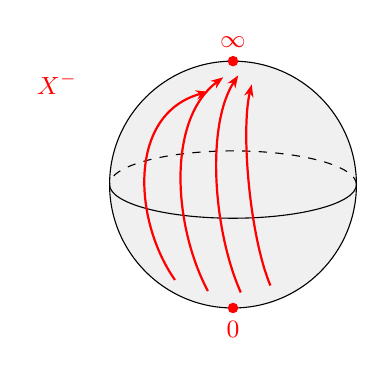
\begin{tikzpicture}[scale=0.95]
  \fill[gray!12] (0,0) circle (1.65);
  \draw (0,0) circle (1.65);
  \draw[dashed] (1.65,0) arc[start angle=0,end angle=180,x radius=1.65,y radius=0.45];
  \draw (1.65,0) arc[start angle=0,end angle=-180,x radius=1.65,y radius=0.45];
  \foreach \a in {-0.33,-0.13,0.07,0.25}{
    \draw[red,thick,-{Stealth[length=4.5pt]}]
      ({2.2*\a-0.05},{-1.45+1.6*\a*\a}) .. controls ({2.7*\a-0.45},{-0.6-0.4*\a})
      and ({2.6*\a-0.55},{0.82-0.4*\a}) .. (\a,{1.47-2.1*\a*\a});}
  \fill[red] (0,1.65) circle (2pt);
  \fill[red] (0,-1.65) circle (2pt);
  \node[red,above] at (0,1.70) {\small $\infty$};
  \node[red,below] at (0,-1.70) {\small $0$};
  \node[red,left] at (-1.95,1.35) {\small $X^-$};
\end{tikzpicture}}

% p.122：例 22.20——$\mathbb G_m$ 在 $\mathbb A^2$ 上的双曲作用
% $t\cdot(a_1,a_2)=(t^{-1}a_1,ta_2)$ 的相图：沿 $x$-轴流出，沿 $y$-轴流入
\expandafter\newcommand\csname figP122\endcsname{%
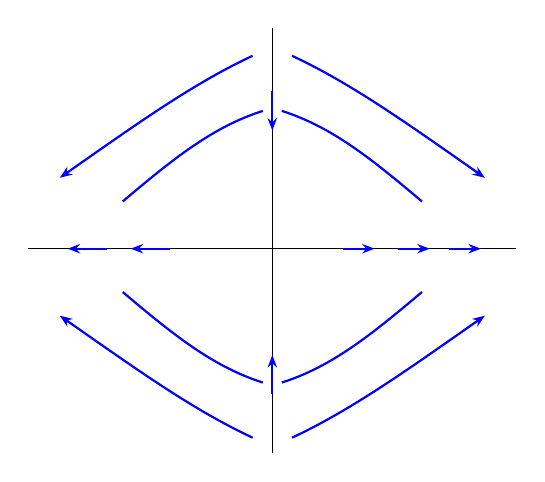
\begin{tikzpicture}[scale=1.0,
  fl/.style={blue,thick,-{Stealth[length=4.5pt]}}]
  \draw (-3.1,0) -- (3.1,0);
  \draw (0,-2.6) -- (0,2.8);
  \foreach \x in {-2.6,-1.8} \draw[fl] (\x+0.5,0) -- (\x,0);
  \foreach \x in {1.3,2.0,2.65} \draw[fl] (\x-0.4,0) -- (\x,0);
  \draw[fl] (0,2.0) -- (0,1.5);
  \draw[fl] (0,-1.85) -- (0,-1.35);
  \foreach \s in {-1,1}{%
    \draw[fl] (0.25*\s,2.45) .. controls (1.0*\s,2.1) and (1.7*\s,1.6) .. (2.7*\s,0.9);
    \draw[blue,thick] (0.12*\s,1.75) .. controls (0.75*\s,1.55) and (1.25*\s,1.15) .. (1.9*\s,0.6);
    \draw[fl] (0.25*\s,-2.4) .. controls (1.0*\s,-2.05) and (1.7*\s,-1.55) .. (2.7*\s,-0.85);
    \draw[blue,thick] (0.12*\s,-1.7) .. controls (0.75*\s,-1.5) and (1.25*\s,-1.1) .. (1.9*\s,-0.55);}
\end{tikzpicture}}

% 转发宏：正文写 \figP{051A}、\figP{121B} 等（\providecommand 便于多批共存）
\providecommand{\figP}[1]{\csname figP#1\endcsname}


\title{\bfseries 局部 Langlands 对应的几何化\\[0.3em]\Large ——Berkeley 讲义}
\author{Peter Scholze 讲授\\Tony Feng 记录\\[0.6em]
  \normalsize 中译注本\quad 译者：数译工程（AI 辅助，详参 \texttt{工程文件/BRIEF.md}）}
\date{底本 148 页（2020-10-30 至 2021-02-12）\quad 译本版本 v1.0}

\begin{document}
\frontmatter
\pagestyle{plain}% 前置件不印页眉
\maketitle
\tableofcontents
\clearpage
% s00-front.tex —— 前置件：译本说明
\chapter*{译本说明}
\addcontentsline{toc}{chapter}{译本说明}

\section*{一、底本}

本译本的底本是 Peter Scholze 于 2020 年秋季至 2021 年春季在 Berkeley 讲授的课程讲义的整理稿：

\begin{quote}
Peter Scholze（讲授），Tony Feng（记录），\emph{Geometrization of the Local Langlands
Correspondence}，2022 年 3 月 19 日生成的 PDF，共 148 页，27 讲附参考文献。
课程自 2020 年 10 月 30 日开始，至 2021 年 2 月 12 日结束；讲次标题后括注的月日即该讲日期。
\end{quote}

底本的印刷页码与 PDF 页码一致（偏移 0）。译本每一页的第一个段落之前都标有原书页码，
读者可据此与底本逐页对照。

\section*{二、体例}

\begin{enumerate}
  \item 术语以本仓库「数译规范」已冻结的译名为准（其中 \emph{perfectoid space} 译「完满空间」，
        \emph{diamond} 译「菱形」）；本库未收录者，参照香蕉空间（\texttt{bananaspace.org}）
        与通行中译取一译名，并在术语表中登记。
  \item 一个英文术语在全书中只对应一个中文译名；术语首次出现时以「中文（English）」形式给出原文。
  \item 人名、定理名、软件名、记号（如 $\Bun_G$、${\Bun_G}$、shtuka 等）不译。
        中文与拉丁字母之间留一个半角空格。
  \item 原文的条目编号（定义、定理、例、注、警告等）由 \LaTeX{} 共用计数器自动生成，
        与底本逐条对应；译文不手写编号。
  \item 公式一律依照底本页面图像重排，不依文本层转写的结果。底本公式偶有排版疏漏，
        凡影响文意者，以译注（脚注形式，标注等级与出处）说明，不改动正文。
\end{enumerate}

\section*{三、说明}

本篇为学术文献的中文译注本，供研读之用；原文著作权归原作者与记录者所有。
底本为作者公开在个人主页上的讲义 PDF，本译本不复制其页面图像，只重排文字与公式。
译文中若有错误，均属译者理解之误，与原作者无关。


\mainmatter
\setcounter{page}{1}
\section[引言]{引言（10 月 30 日）}
\srcpage{2}

本课程讲的是与 Laurent Fargues 的合作工作。

\subsection{设定}

设 $E$ 为非阿基米德局部域，即 $E=\mathbb{F}_q((t))$ 或 $\mathbb{Q}_p$ 的有限扩域。我们引入一些记号：
\begin{itemize}
  \item $\mathbb{F}_q$ 是 $E$ 的剩余域。
  \item $\pi\in\mathcal{O}_E$ 是一致化子。
  \item $G/E$ 是约化群，例如 $G=\mathrm{GL}_n$、$\mathrm{Sp}_{2n}$。（这个理论的一部分吸引力在于：它对任意约化群都完全一致地成立。）
\end{itemize}

我们关心局部投射有限群（locally profinite group）$G(E)$ 的表示论。下面简要回忆其中一些事实。

\subsection{$p$ 进群的表示}

设 $\Gamma$ 为局部投射有限群。

\begin{definition}
域 $L$ 上 $\Gamma$ 的一个光滑表示（smooth representation）\footnote{也许「局部常值」是更好的术语……}是一个 $L$-向量空间 $V$，连同映射 $\Gamma\to\mathrm{GL}(V)$，使得对一切 $v\in V$，$\mathrm{Stab}(v)\subseteq\Gamma$ 都是开子群。
\end{definition}

\begin{example}
设 $K\subset G(E)$ 为开紧子群。由于 $K$ 投射有限，它有很多有限商。设有这样的有限商 $K\twoheadrightarrow\bar K$ 以及表示 $\rho:\bar K\to\mathrm{GL}(V_0)$。于是可以作紧诱导
\[
c\text{-}\Ind_K^\Gamma(\rho)=\{f:\Gamma\to V_0\mid f\ \text{有紧支撑},\ f(gk)=f(g)k\quad\forall g\in\Gamma,\ k\in K\}.
\]
若 $L$ 的特征为零，这些对象是光滑表示范畴的紧投射生成元。
\end{example}

\begin{example}[紧诱导]
设 $K=\mathrm{GL}_n(\mathcal{O}_E)\subset\Gamma=\mathrm{GL}_n(E)$，$\bar K=\mathrm{GL}_n(\mathbb{F}_q)$，$\rho$ 为 $\mathrm{GL}_n(\mathbb{F}_q)$ 的尖点表示（cuspidal representation）。则 $c\text{-}\Ind_K^\Gamma\rho$ 是「超尖点」表示，在固定中心特征标之后不可约。
\end{example}

\begin{example}[抛物诱导]
若 $P\subset G$ 是以 $L$ 为 Levi 的抛物子群，且 $(V_0,\rho_L)$ 是 $L(E)$ 的光滑表示，则
\[
\Ind_{P(E)}^{G(E)}V_0=\{f:G(E)\to V_0\mid f(\gamma p)=f(\gamma)p\quad\forall\gamma\in G(E),\ p\in P(E)\}
\]
是 $G(E)$ 的光滑表示。超尖点表示就是不出现在这种表示中的表示。在某种模糊的意义上，$G(E)$ 的所有不可约光滑表示都由 Levi 子群的超尖点表示经抛物诱导构造出来。
\end{example}

\begin{example}[自守表示]
若 $\mathbb{E}$ 为整体域，$\mathbb{G}$ 为 $\mathbb{E}$ 上的约化群，使得 $(G,E)$ 作为 $(\mathbb{G},\mathbb{E})$ 的局部化出现，则自守形式空间
\[
\mathcal{A}\bigl(\mathbb{G}(\mathbb{E})\backslash\mathbb{G}(\mathbb{A}_{\mathbb{E}}),\mathbb{C}\bigr)
\]
是 $G(E)$ 的光滑表示。\yizhu{原文把 $(G,E)$ 与 $(\mathbb{G},\mathbb{E})$ 写成同一记号；按文意后者应为 $(\mathbb{G},\mathbb{E})$。}{A（原文 p.2）}
\end{example}

在某种意义上，对 $G(E)$ 的光滑表示范畴的研究，是研究自守形式空间的局部类比。

\srcpage{3}

\subsection{局部 Langlands 对应}

现在叙述局部 Langlands 猜想的一个多少不太精确的形式。为简单起见，设 $G$ 分裂。

\begin{conjecture}[Langlands]
考虑 $L=\mathbb{C}$ 上的表示。存在「自然的」映射
\[
\mathrm{Irrep}(G(E))/\sim\ \longrightarrow\ \mathrm{Hom}(W_E,\widehat{G}(\mathbb{C}))/\widehat{G}(\mathbb{C})\text{-conj},
\]
其中 $\widehat{G}$ 是 Langlands 对偶群，$W_E$ 是 $E$ 的 Weil 群\footnote{这是 $\mathbb{Z}\subset\widehat{\mathbb{Z}}$ 在满射 $\Gal(\bar E/E)\to\widehat{\mathbb{Z}}$ 下的原像，该满射对应 $E$ 的最大无分歧扩域。}；该映射满射，且纤维有限（纤维称为 $L$-包）。
\end{conjecture}

\begin{remark}
猜想有更精细的版本，能精确描述这些纤维。近来还有一些改进，它们猜想性地用 Artin 叠 $\mathrm{Hom}(W_E,\widehat{G}(\mathbb{C}))/\widehat{G}(\mathbb{C})$ 上的凝聚层来刻画整个范畴 $\Rep(G(E))$。
\end{remark}

以下是我最初想到的几个问题。
\begin{enumerate}[label=(\arabic*)]
  \item 这为什么说得通——$W_E$ 与 $\Rep(G(E))$ 之间如何相关？
  \item $\widehat{G}$ 从何而来？
\end{enumerate}

为进一步讨论 (2)，先回忆 $\widehat{G}$ 是什么。回忆：任意域上的分裂约化群 $G$ 由根数据 $(X,\Phi,X^*,\Phi^\vee)$ 分类。一个有趣的观察是：$(X^*,\Phi^\vee,X,\Phi)$ 也是根数据，它定义了 $\widehat{G}$。

\begin{example}[一些对偶群]
$\widehat{\mathrm{GL}}_n=\mathrm{GL}_n$，$\widehat{\mathrm{SL}}_n=\mathrm{PGL}_n$，$\widehat{\mathrm{Sp}}_{2n}=\mathrm{SO}_{2n+1}$，$\widehat{\mathrm{SO}}_{2n}=\mathrm{SO}_{2n}$。
\end{example}

\subsection{局部 Langlands 对应的例子}

\subsubsection{$G=\mathbb{G}_m$}

当 $G=\mathbb{G}_m$ 时，$G(E)=E^\times$ 交换，故 $\mathrm{Irrep}(E^\times)=\{\chi:E^\times\to\mathbb{C}^\times\}$ 是特征标的集合。对偶群为 $\widehat{G}=\mathbb{G}_m$，并且
\[
\mathrm{Hom}(W_E,\widehat{G}(\mathbb{C}))=\mathrm{Hom}(W_E,\mathbb{C}^\times)=\mathrm{Hom}(W_E^{ab},\mathbb{C}^\times).
\]
事实上，局部类域论给出同构 $E^\times\xrightarrow{\sim}W_E^{ab}$。

\subsubsection{$G=\mathrm{GL}_n$}

当 $G=\mathrm{GL}_n$ 时，对偶群为 $\widehat{G}=\mathrm{GL}_n$。

\begin{theorem}[Laumon--Rapoport--Stuhler, Harris--Taylor, Henniart]
$\mathrm{GL}_n(E)$ 的超尖点表示与 $W_E\to\mathrm{GL}_n(\mathbb{C})$ 的不可约 $n$ 维表示之间存在「自然的」双射。
\end{theorem}

这还没有给出 $\mathrm{Irrep}(\mathrm{GL}_n(E))/\sim$ 与 $\mathrm{Hom}(W_E,\widehat{G}(\mathbb{C}))$ 之间的自然双射，但用 Bernstein--Zelevinsky 可以确切说出会发生什么。

\begin{example}[自守诱导]
与 $n=1$ 的情形不同，实践中在 Galois 一侧写下对象更容易。设 $E'/E$ 为 $n$ 次扩域，$\chi':W_{E'}\to W_{E'}^{ab}\cong(E')^\times\to\mathbb{C}^\times$ 为一般特征标，则 $\varphi:=\Ind_{W_{E'}}^{W_E}(\chi')$ 是 $W_E$ 的不可约 $n$ 维表示。它应当对应 $\mathrm{GL}_n(E)$ 的一个超尖点表示 $\pi_\varphi$。直接构造 $\pi_\varphi$ 相当困难。
\end{example}

\begin{remark}
局部 Langlands 对应的许多显式例子已由 Bushnell、Kutzko、Kaletha 等人的工作给出。它极其复杂！
\end{remark}

\subsection{本课程的目标}

\srcpage{4}

\subsubsection{}

第一个目标是给出映射 $\pi\mapsto\varphi_\pi$ 的构造：从不可约表示到 $L$-参数，它对任意约化群 $G$ 都一致地成立，并且是纯粹局部的。

\begin{remark}[相关工作]
在函数域情形，这基本上已由 Genestier--Lafforgue 完成。对 $\mathrm{GL}_n$，证明走的是整体方法。此后 Jim Arthur 用扭内视（twisted endoscopy）把它推广到经典群。
\end{remark}

\subsubsection{}

第二个目标是「解释」$W_E$ 与 $\widehat{G}$ 从哪里来。

\subsubsection{}

第三个目标是把局部 Langlands 对应表述为范畴的等价这种更有结构的形式，并（本质上）构造一个方向上的函子。这使陈述精确得多：我们构造的这个函子就是等价。

\begin{remark}[系数]
这些方法对任意满足 $p\in\Lambda^\times$ 的系数环 $\Lambda$ 都适用。
\end{remark}

\subsection{粗略的想法}

我们想在「Fargues--Fontaine 曲线」上发展几何 Langlands 纲领，使用「完满空间/菱形」的几何。

我们无法详细回顾所有这些主题。参考文献包括：
\begin{itemize}
  \item \emph{Berkeley lectures on $p$-adic geometry}.
  \item \emph{Lecture notes for Montreal workshop}.
\end{itemize}

\subsection{整体图景}

我们想审视空间「$\Spec E$」。看待一个概形有几种不同的方式。
\begin{itemize}
  \item 一种是通过它的 étale 拓扑；在 $\Spec E$ 的情形，它由 $\pi_1^{\et}(\Spec E)=\Gal(\bar E/E)$ 掌控。
  \item 另一种是通过凝聚层。在这里，凝聚层就只是 $E$-向量空间。更一般地，可以考虑 $G$-主丛的群胚
  \[
  [\mathrm{pt}/G](\Spec E)=\coprod_{\alpha\in H^1(E,G)}[\mathrm{pt}/G_\alpha(E)],
  \]
  其中 $G_\alpha(E)$ 是对应于主丛 $\alpha$ 的内形式。特别地，$[\mathrm{pt}/G(E)]$ 作为开闭子叠落在其中，且 $\Rep(G(E))=\mathrm{Shv}([\mathrm{pt}/G(E)])$ 自然地嵌入 $\mathrm{Shv}([\mathrm{pt}/G](\Spec E))$。我们会发现，研究这个更大的范畴是有益的\footnote{这个想法也受到 Vogan 与 Bernstein 的强调。}。
\end{itemize}

现在我们要把这个图景稍作修改。我们想把 $\Gal(\bar E/E)$ 换成 $W_E$。对 $\mathbb{F}_q$ 上的概形 $X$，我们用带 $\Frob_q$ 作用的 $X_{\overline{\mathbb{F}}_q}$ 替换 $X$。此时 $\pi_1(X_{\overline{\mathbb{F}}_q}/\Frob_q)=\pi_1(X_{\overline{\mathbb{F}}_q})\rtimes\mathbb{Z}$ 是基本群的「Weil 形式」。

在我们的情形，这提示把
\begin{itemize}
  \item $\Spec\mathbb{F}_q((t))$ 换成「$\overline{\mathbb{F}}_q((t))/\Frob_q$」；
  \item $\Spec E$ 换成 $\Spec\breveE/\Frob_q$，其中 $\breveE$ 是 $E$ 的最大无分歧扩域的完备化。
\end{itemize}

现在改为考虑「$\Spec\breveE/\Frob_q$」的图景：
\begin{itemize}
  \item étale 侧由 $\pi_1(\Spec\breveE/\Frob_q)=W_E$ 掌控。
  \item \srcpage{5}凝聚侧，向量丛按下降就是等晶体（isocrystal）的范畴
  \[
  \Isoc_E=\{\breveE\text{-向量空间}+\text{Frob-半线性}\ \varphi:V\xrightarrow{\sim}V\}.
  \]
  这比单纯的 $E$-向量空间丰富。由 Dieudonné--Manin 定理，它分解为
  \[
  \bigoplus_{\lambda\in\mathbb{Q}}\Isoc_E^\lambda,
  \]
  其中 $\Isoc_E^\lambda$ 由斜率为 $\lambda$ 的纯等晶体组成。范畴 $\Isoc_E^\lambda$ 可以等同于 $D_\lambda$-模，其中 $D_\lambda/E$ 是不变量为 $[\lambda]\in\mathbb{Q}/\mathbb{Z}$ 的中心除代数。

  更一般地，可以考虑 $\Isoc_E$ 中 $G$-主丛的范畴。这由 Kottwitz 分类，动机来自 Shimura 簇的理论。他证明 $G$-等晶体的群胚是
  \[
  \coprod_{b\in B(E,G)}[\mathrm{pt}/G_b(E)],
  \]
  其中 $G_b$ 是 $G$ 的某个 Levi 子群的内形式。有单射 $H^1(E,G)\hookrightarrow B(E,G)$。Kottwitz 和 Kaletha 已经从纯表示论的视角意识到，同时考虑所有 $G_b$ 是有益的。
\end{itemize}

\subsection{等晶体叠}

我们想要比 $\coprod_{b\in B(E,G)}[\mathrm{pt}/G_b(E)]$ 更具几何性的东西。我们想把它提升为「$G$-等晶体叠」，对此有几种做法。

\subsubsection{}

$\Isoc_E$ 是 $E$-线性范畴，故对任意 $E$-代数 $A$ 都可以考虑 $\Isoc_E\otimes_E A$ 中的 $G$-主丛。这导出 $E$ 上的一个 Artin 叠，即
\[
\coprod_{b\in B(E,G)}[\mathrm{pt}/G_b].
\]
我们强调，这里 $G_b$ 是代数群，而这一观点对于看出 $G_b$ 可以提升为代数群至关重要。但从我们的视角看，这并不是正确的做法，因为我们追求的是 $p$ 进群的光滑表示，而不是代数群的代数表示。

\subsubsection{}

更好的想法是把 $\overline{\mathbb{F}}_q$ 换成任意（完美）$\overline{\mathbb{F}}_q$-代数 $R$\yizhu{本译本把 perfect 译作「完美」，以与 perfectoid 的定译「完满」相区分。}{I（本库 SY02-16 术语表：perfectoid=完满）}，即把
\begin{gather*}
\Spec\overline{\mathbb{F}}_q((t))/\Frob_q\ \rightsquigarrow\ \Spec R((t))/\Frob_q,\\
\Spec\breveE/\Frob_q\ \rightsquigarrow\ \Spec(W(R)\otimes_{W(\overline{\mathbb{F}}_q)}E)/\Frob_q.
\end{gather*}
我们可以在完美 $\overline{\mathbb{F}}_q$-代数上定义叠
\[
R\mapsto\bigl\{G\text{-主丛}: \Spec R((t))/\Frob_q\ \text{或}\ \Spec(W(R)\otimes_{W(\overline{\mathbb{F}}_q)}E)/\Frob_q\bigr\}.
\]
结果表明，这是一个性态良好的叠，我们称之为 $G-\Isoc$\footnote{$G-\Isoc$ 等价于 Gaitsgory、Genestier--Lafforgue、Zhu 考察过的对象「${}^{L}G/_{\sigma}{}^{L}G$」。他们给出 $D(G-\Isoc,\Ql)$ 到各分片 $D(G-\Isoc^b,\Ql)\cong D(G_b(E),\Ql)$ 的半正交分解。}。

\srcpage{6}

\begin{theorem}[Rapoport--Richartz, Caraiani--Scholze, Ivanov, Anschütz]
$G-\Isoc$ 是 $v$/arc 拓扑下的叠\footnote{这甚至强于在 fpqc 拓扑下成为叠！}。

对任意 $b\in B(E,G)$，存在局部闭子叠 $G-\Isoc^b\subset G-\Isoc$，在其上等晶体同构于 $b$，并且 $G-\Isoc^b\cong[\mathrm{pt}/G_b(E)]$\footnote{这构成一个分层，但各层不是开闭的（粘合数据很复杂）。}。
\end{theorem}

\subsubsection{}

我们仍然不会完全考虑这个叠。我们要考虑一个更解析的版本，它可以说性态更好，用完满环（perfectoid ring）代替完美代数。

为说明动机，我们指出：与 Langlands 对偶群 $\widehat{G}$ 的联系是通过 Hecke 算子。

我们把 $R((t))$ 看成一个小的去心圆盘。我们要考虑 $G$-主丛空间上的对应。

我们考虑参数化如下数据的空间：$(\Spec R((t))/\Frob_q)$ 上的两个 $G$-主丛 $\mathcal{E}_1,\mathcal{E}_2$，以及它们在某个除子 $D\subset\Spec R((t))$ 之外的同构 $\mathcal{E}_1\cong\mathcal{E}_2$。这需要截面 $\Spec R\to\Spec R((t))$，而当 $R$ 是离散环时这样的截面不存在。所以我们需要取 $R$ 为 Banach 代数。这促成了完满几何的登场。

对 $\overline{\mathbb{F}}_q$ 上任意完满 affinoid 代数 $(R,R^+)$，可以联系 Fargues--Fontaine 曲线 \mbox{$\mathbb{D}^*_{\Spa(R,R^+)}/\Frob_q$}（或混合特征下的类似对象）。于是可以考虑 Fargues--Fontaine 曲线上 $G$-主丛的模空间。

解析情形的优点是去心圆盘要几何得多。因此我们真的可以考虑 Hecke 算子
\[
\begin{tikzcd}
& \Hck_G \arrow[dl, "\mathrm{pr}_1"'] \arrow[dr, "\mathrm{pr}_2"] & \\
\Bun_G & & \Bun_G\times(\Spa\,\breveE/\phi)
\end{tikzcd}
\]
这里 $\Spa(\breveE/\phi)$ 是参数化 Fargues--Fontaine 曲线截面的空间。

$\Hck_G$ 是无穷维的，但它有有限维的层（strata）$\Hck_G^\mu$。令
\[
T_\mu:=\mathrm{pr}_{2!}\mathrm{pr}_1^*:D(\Bun_G,\Ql)\to D(\Bun_G\times\Spa\,\breveE/\phi;\Ql)=D(\Bun_G,\Ql)^{W_E}.
\]
几何 Satake 等价说，算子 $T_\mu$ 由 $\Rep(\widehat{G})$ 枚举。回忆 $D(\Bun_G,\Ql)$ 是诸 $\Rep(G_b(E);\Ql)$ 的某种汇总。结果表明，要定义附加在 $\Rep(G_b(E);\Ql)$ 上的 $L$-参数，恰恰需要这种范畴结构。
\section[Fargues--Fontaine 曲线 I]{Fargues--Fontaine 曲线 I（11 月 2 日）}
\srcpage{7}

\subsection{局部域}

固定一个非阿基米德局部域 $E$，其剩余域是特征为 $p$ 的 $\mathbb{F}_q$。设 $\pi\subset\mathcal{O}_E$ 为一个一致化子（uniformizer）\yizhu{原文如此，此处应为 $\pi\in\mathcal{O}_E$。}{A（原文 §2.1 p.7）}。

\begin{example}
具体地说，或者 $E\cong\mathbb{F}_q((t))$，或者 $E$ 是 $\mathbb{Q}_p$ 的有限扩张。
\end{example}

目标是「把 $\Spec E$ 几何化」。

\begin{itemize}
  \item $\Spec E$ 的 Zariski 网站是一个点，这不太几何——我们要把它加强。
  \item $E$ 的 étale 网站是 $\{\text{有限可分}\ E\text{-代数}\}^{\mathrm{op}}$。换言之，它是 $B\Gal(\overline{E}/E)$，
        也可以看作带连续 $\Gal(\overline{E}/E)$-作用的有限集合范畴。这更有趣，但仍然不太几何。
\end{itemize}

我们有一个短正合列
\[
\begin{tikzcd}[column sep=2.4em, row sep=1.4em]
0 \arrow[r] & I_E \arrow[r] & \Gal(\overline{E}/E) \arrow[r]
  & \Gal(\overline{\mathbb{F}}_q/\mathbb{F}_q) \arrow[r] \arrow[d, "\sim"] & 1 \\
  & & & \widehat{\mathbb{Z}}=\langle\Frob_q\rangle &
\end{tikzcd}
\]
并且惯性子群 $I_E$ 还可以进一步分解为
\[
0\to P_E\to I_E\to\prod_{\ell\ne p}\mathbb{Z}_\ell\to0 .
\]

\subsubsection{局部 Tate 对偶}

若 $E$ 的特征为 $0$，则对一切挠 $\Gal(\overline{E}/E)$-表示 $M$，有配对
\[
H^i_{\et}(\Spec E,M)\otimes H^{2-i}_{\et}(\Spec E,M^*(1))
\longrightarrow H^2_{\et}(\Spec E,\mathbb{Q}/\mathbb{Z}(1))=\mathbb{Q}/\mathbb{Z}.
\]
这里 $M^*=\Hom(M,\mathbb{Q}/\mathbb{Z})$，而 $\mathbb{Q}/\mathbb{Z}(1)$ 是 Tate 扭，即 $\bigcup_n\mu_n$。
若 $E$ 的特征为 $p$，则我们把讨论限制在 prime-to-$p$ 的 $M$ 与 $\mathbb{Q}/\mathbb{Z}$ 中的 prime-to-$p$ 挠部分上。

这看起来像 2 维流形上的 Poincaré 对偶。（但 Tate 扭意味着它的定向层非平凡。）
我们想把 $\Spec E$ 变成更接近紧 Riemann 曲面的东西。

\subsection{等特征的 Fargues--Fontaine 曲线}

设 $E=\mathbb{F}_q((t))$，并令 $\breve E=\overline{\mathbb{F}}_q((t))$。直观上，$\Spec\overline{\mathbb{F}}_q((t))$ 是
「$\overline{\mathbb{F}}_q$ 上的形式去心开单位圆盘（formal punctured open unit disc）」。但它当然只有一个点。
我们将通过过渡到扩域来「造出更多空间」。

取 $C/\overline{\mathbb{F}}_q$ 为完备代数闭非阿基米德域，例如 $C=\overline{\mathbb{F}}_q((u))^\wedge$。考虑 adic 谱
$\Spa C\times_{\Spa\mathbb{F}_q}\Spa\mathbb{F}_q((t))$。这就是「$C$ 上的去心开单位圆盘」
\[
\mathbb{D}^*_C=\{x\mid 0<|x|<1\}.
\]
它现在有许多点。

基变换到 $C$ 相当于过渡到「几何」的情形；正如前几讲那样，我们要记住 Frobenius $\varphi_C$。

\begin{definition}
（关于 $E,C$ 的）\emph{Fargues--Fontaine 曲线}\footnote{这依赖于 $C$ 的选取。}是
$X_{C,E}:=\mathbb{D}^*_C/\varphi_C^{\mathbb{Z}}$，视作 $E$ 上的 adic 空间。
\end{definition}

\srcpage{8}

\begin{remark}
$\varphi_C^{\mathbb{Z}}$ 在 $\mathbb{D}^*_C$ 上的作用自由。因此这个商的性质非常好。
然而要注意：尽管 $\mathbb{D}^*_C$ 是 $C$ 上的有限型对象，由于作用在底 $C$ 上非平凡，它不再生活在 $C$ 上；
它反而是 $E$ 上的无限型对象。
\end{remark}

这在何种意义上是对 $\Spec E$ 的几何化？下面这些性质归功于 Fargues--Fontaine。
\begin{itemize}
  \item $H^0(X_{C,E},\mathcal{O}_{X_{C,E}})=E$。
  \item $X_{C,E}$ 的有限 étale 覆盖的范畴是 $(\Spec E)_{\et}$。
  \item $H^i_{\et}(X_{C,E},M)\cong H^i_{\et}(\Spec E,M)$。
\end{itemize}
特别地，局部 Tate 对偶变成 $X_{C,E}$ 上的整体对偶。

\subsection{关于 adic 空间的一些回顾}

粗略地说，adic 空间是联系于某些拓扑环（例如 Banach 代数）的概形变体。它们与概形的共同之处在于：
\begin{itemize}
  \item 点之间有特殊化关系。
  \item 它们非常一般：基础部分没有任何有限性假设（这点与刚性解析几何不同）。
\end{itemize}

\begin{definition}
设 $A$ 是拓扑环。
\begin{enumerate}[label=(\arabic*), leftmargin=2.6em]
  \item 称 $A$ 是 \emph{adic} 的，若存在理想 $I\subseteq A$，使得 $\{I^n\mid n\ge0\}$ 是 $0$ 的邻域基。
        这样的理想 $I$ 称为\emph{定义理想}（ideal of definition）。
        （它并不唯一；但对任意两个 $I,J$，存在 $n$ 使得 $I^n\subset J$ 且 $J^n\subset I$。）
  \item 称 $A$ 是 \emph{Huber} 的\footnote{在 Huber 的原始论文中，这被称为「$f$-adic」。}，
        若存在开子环 $A_0\subset A$，它是定义理想为有限生成的 adic 环。
        这样的 $A_0\subseteq A$ 称为\emph{定义环}（ring of definition）。
\end{enumerate}
\end{definition}

\begin{remark}
任何这样的 $A$ 都有完备化 $\widehat{A}$，它包含 $I$-adic 完备化 $\widehat{A}_0\subset\widehat{A}$ 作为开子环。
\end{remark}

对我们最重要的一类 adic 环是：

\begin{definition}
若 $A$ 含有一个拓扑幂零单位 $\varpi\in A$，则称 $A$ 是 \emph{Tate 环}。
这样的 $\varpi$ 称为\emph{伪一致化子}（pseudouniformizer）。
\end{definition}

\begin{example}
任何非阿基米德域都是 Tate 的。在 $\mathbb{F}_p((t))$ 中可取 $\varpi=t$；在 $\mathbb{Q}_p$ 中可取 $\varpi=p$。
更一般地，非阿基米德局部域上的任何 Huber 环都是 Tate 的。
\end{example}

\begin{remark}
设 $K$ 是任意非阿基米德局部域，$\varpi\in K$ 是伪一致化子，$A/K$ 是完备 Huber 环。
则 $A$ 自然地具有 $K$ 上 Banach 代数的结构，其「单位球」为
$\{f\in A:|f_0|\le1\}=A_0$\yizhu{原文下标作 $|f_0|$，疑为笔误，当作 $|f|\le1$。}{A（原文 §2.2 p.8）}。
任何定义环 $A_0\subset A$ 都带有 $\varpi$-adic 拓扑。
\end{remark}

$A$ 上的范数可以这样构造：任取 $\|\varpi\|$ 为 $(0,1)$ 中的某个实数，然后定义
\[
\|a\|=\inf_{\{n\mid\varpi^na\in A_0\}}2^n .
\]

$K$ 上带连续映射的 Banach 代数与 $K$ 上的 Tate--Huber 环之间有范畴等价。
所以我们本可以用 Banach 代数而不是 Tate 环来表述。但 Tate 环的进路至少有两点好处：
\begin{itemize}
  \item 我们不需要固定一个非阿基米德的基域 $K$。
  \item \srcpage{9}范数本身是多余的结构。
\end{itemize}

\begin{definition}
Huber 环 $A$ 的\emph{赋值谱}（valuation spectrum）是
\[
\mathrm{Cont}(A):=\{\text{连续赋值}\ |\cdot|:A\to\Gamma\cup\{0\}\}/\sim,
\]
其中 $\Gamma$ 是全序交换群（例如 $\mathbb{R}_{>0}$）。
我们在 $\mathrm{Cont}(A)$ 上取由开集 $\{|f|\le|g|\ne0\}\subset\mathrm{Cont}(A)$（$f,g\in A$）生成的拓扑。
\end{definition}

具体来说，「连续赋值」是指：
\begin{itemize}
  \item $|ab|=|a|\cdot|b|$，$0\gamma=\gamma0=0$，且对一切 $\gamma$ 有 $0\le\gamma$。
  \item $|a+b|\le\max(|a|,|b|)$。
  \item $|0|=0$，$|1|=1$。
  \item 对一切 $\gamma\in\Gamma$，$\{a\mid |a|<\gamma\}\subset A$ 是开集。
\end{itemize}

两个连续赋值 $|\cdot|_1,|\cdot|_2$ 称为\emph{等价}的，若它们给出的二元关系相同：
\[
|a|_1\ge|b|_1\iff|a|_2\ge|b|_2 .
\]
这等价于：若 $\Gamma_i$ 取得极小，则存在同构 $\Gamma_1\xrightarrow{\sim}\Gamma_2$，使得下图交换。
\[
\begin{tikzcd}[column sep=3.2em, row sep=1.8em]
  & \Gamma_1\cup\{0\} \arrow[dd, "\sim"] & \\
A \arrow[ru, "|\cdot|_1"] \arrow[rd, "|\cdot|_2"'] & & \\
  & \Gamma_2\cup\{0\} &
\end{tikzcd}
\]

\begin{example}
若 $\Gamma$ 可嵌入 $\mathbb{R}_{>0}$，则称该赋值是「秩 $1$」的。
一个自然出现、且不是秩 $1$ 的 $\Gamma$ 的例子是 $\mathbb{R}_{>0}\times\gamma^{\mathbb{Z}}$，
其中对一切 $r\in\mathbb{R}_{>1}$ 都有 $r>\gamma>1$。
\end{example}

\begin{example}
定义中的严格性只在 $\Gamma=\{1\}$ 时才起作用。
\end{example}

\begin{definition}
一个 \emph{Huber 对}（Huber pair）是一对 $(A,A^+)$，其中 $A$ 是 Huber 环，
$A^+\subset A$ 是由幂有界（power-bounded）元素构成的、开的整闭子环。
记 $A^\circ\subset A$ 为幂有界元素构成的子环。
\end{definition}

我们定义
\[
\Spa(A,A^+)=\{|\cdot|:|A^+|\le1\}\subset\mathrm{Cont}(A),\qquad
\Spa A=\Spa(A,A^\circ).
\]

我们可以在有理子集组成的基上，给 $\Spa A$ 配备 Huber 环的预层
$\mathcal{O}_{\Spa A}\supset\mathcal{O}^+_{\Spa A}$。这里的有理子集（rational subsets）形如
\[
U\Bigl(\frac{f_1,\dots,f_n}{g}\Bigr):=\bigl\{|f_i|\le|g|\ne0\bigr\},
\]
其中 $(f_1,\dots,f_n,g)$ 生成一个开理想。于是
\[
\mathcal{O}_{\Spa A}\Bigl(U\Bigl(\frac{f_1,\dots,f_n}{g}\Bigr)\Bigr)
=A\Bigl\langle\frac{f_1}{g},\dots,\frac{f_n}{g}\Bigr\rangle
\]
「允许 $f_i/g$ 的一切收敛级数」。$+$ 子环的作用是记录哪些元素 $\le1$，所以它包含 $f_i/g$。
子环 $\mathcal{O}^+_{\Spa A}\bigl(U(\frac{f_1,\dots,f_n}{g})\bigr)$ 是包含 $A^+$ 与所有 $f_i/g$ 的最小子环。

\begin{theorem}[Huber 等]
在一切实际情形中，$\mathcal{O}_{\Spa(A,A^+)}$ 都是层，但并非总是如此。
\end{theorem}

\srcpage{10}
\begin{center}
\figP{010}
\end{center}

\begin{remark}
最近人们认识到（Bambozzi--Kremnizer、Clausen--S），这种非层性可以通过允许结构层取导出对象来修正。
微妙之处在于如何把导出色性与拓扑结合起来；我们与 Clausen 借助凝聚态（condensed）数学的理论解决了这一点。
这与本课程无关。
\end{remark}

\begin{definition}
一个 \emph{adic 空间}是一个三元组 $(X,\mathcal{O}_X,\mathcal{O}^+_X)$，其中
\begin{itemize}
  \item $X$ 是拓扑空间，
  \item $\mathcal{O}_X$ 是完备拓扑环的层，
  \item $\mathcal{O}^+_X$ 是 $\mathcal{O}_X$ 的子层，
\end{itemize}
它在局部上形如 $(\Spa(A,A^+),\mathcal{O}_A,\mathcal{O}^+_A)$，再加上「局部环化」的正确类比。
\end{definition}

\begin{remark}
这也可以等价地表述为：给出 $\mathcal{O}_X$ 的茎上的赋值，而不是给出 $\mathcal{O}^+_X$。
子层 $\mathcal{O}^+_X\subset\mathcal{O}_X$ 可以还原为那些在所有点处的赋值都 $\le1$ 的元素。
\end{remark}

\begin{remark}
为什么我们要求 $\mathcal{O}_X$ 是完备环的层？一个好处是：只有借助完备的对象，
我们才能表述有理子集上函数 $A\langle\frac{f_1}{g},\dots,\frac{f_n}{g}\rangle$ 的良好泛性质。
\end{remark}

\begin{example}
设 $C$ 是非阿基米德域。我们来解释 $\mathbb{D}^*_C=\{x\mid0<|x|<1\}$ 上的 adic 空间结构。有 Tate 代数
\[
C\langle T\rangle=\Bigl\{\sum a_nT^n \mid a_n\in C,\ a_n\to0\Bigr\}.
\]
于是 $\Spa C\langle T\rangle=:\mathbb{B}_C$ 是 $C$ 上的「闭单位圆盘」$\{x\mid0\le|x|\le1\}$。
我们有 $\mathbb{B}^*_C=\mathbb{B}_C\setminus\{0\}=\bigcup_{\epsilon>0}\mathbb{A}(\epsilon,1)$，
其中非正式地说，对 $\epsilon\in|C|$，$\mathbb{A}(\epsilon,1)$ 就是环带 $\{x\mid\epsilon\le|x|\le1\}$。
更形式地说，$\mathbb{A}(\epsilon,1)=\Spa A_\epsilon$，其中
\[
A_\epsilon=\Bigl\{\sum_{n=-\infty}^{\infty}a_nT^n:\ a_n\in C,\
|a_n|\xrightarrow[n\to\infty]{}0,\ \epsilon^n|a_n|\xrightarrow[n\to-\infty]{}0\Bigr\}.
\]
类似地，$\mathbb{D}^*_C=\bigcup_{\epsilon>0,\,r<1}\mathbb{A}(\epsilon,r)$，其中
$\mathbb{A}(\epsilon,r)=\{\epsilon\le|T|\le r\}$。
\end{example}

\begin{warning}
$\mathbb{D}^*_C\subset\mathbb{B}_C$ 是开的，但它不等于 $\{0<|T|<1\}$。
存在一个点 $x\in\mathbb{B}_C=\Spa\langle T\rangle$，使得对一切 $r\in|C|$（$r<1$）都有 $r<|T(x)|<1$，
即 $x$ 无穷小地小于 $1$。递增的环带并集不包含这样的点。
子集 $\{0<|T|<1\}$ 不是开的，因为严格不等式 $<1$ 定义的是闭子集。
\end{warning}

\srcpage{11}
\begin{center}
\figP{011-1}
\end{center}
\begin{center}
\figP{011-2}
\end{center}

事实上存在自然的映射 $\mathrm{rad}:\mathbb{B}_C\to[0,1]$ 与 $\mathrm{rad}:\mathbb{D}^*_C\to(0,1)$，
它们都把 $x$ 送到 $|T(\tilde x)|$。Frobenius $\varphi_C$ 把 $\mathbb{D}^*_C$ 从原点向外移动，即
$\mathrm{rad}\circ\varphi_C=\mathrm{rad}^{1/q}$。

这说明 $\varphi_C$ 在 $\mathbb{D}^*_C$ 上的作用自由且真不连续（properly discontinuous）。
因此可以定义 $X_{C,E}=\mathbb{D}^*_C/\varphi_C^{\mathbb{Z}}$。
这可以看作 $\mathbb{A}(r,r^{1/q})$ 模去经由 $\phi:\mathbb{A}(r,r)\cong\mathbb{A}(r^{1/q},r^{1/q})$
对边界环带所作的等同。

直觉上，这个商看起来有点像复环面。
\section[Fargues--Fontaine 曲线 II]{Fargues--Fontaine 曲线 II（11 月 5 日）}
\srcpage{12}

\subsection{回顾}

上次我们考虑了等特征局部域 $E=\mathbb{F}_q((t))$ 的 Fargues--Fontaine 曲线。

设 $C/\mathbb{F}_q$ 是完备代数闭非阿基米德域，我们考虑了
\[
\Spa E\times_{\Spa\mathbb{F}_q}\Spa C=\mathbb{D}^*_C,
\]
即 $C$ 上的去心开单位圆盘。它有 $\varphi_C$ 的作用，而我们定义了
$X_{C,E}:=\mathbb{D}^*_C/\varphi_C^{\mathbb{Z}}$。

\subsection{经典点}

有范畴等价
\[
\{\text{刚性解析簇}/C\}\cong\{\text{「局部有限型」adic 空间}/\Spa C\}.
\]
该等价由 $X(C)\leftarrow X$ 给出，其中 $X(C)\subset|X|$ 是「经典点」。
局部地 $X=\Spa A$，其中 $A=C\langle T_1,\dots,T_n\rangle/I$，并且
\[
X(C)=\{(x_1,\dots,x_n)\in C^n: |x_i|\le1,\ f(x_1,\dots,x_n)=0\}=:|\mathrm{Sp}\,A|.
\]

Tate 定义了 Grothendieck 拓扑 $(\mathrm{Sp}\,A)_{\mathrm{rig}}$，它由「拟紧容许开集」组成，
等价于 $\Spa A$ 上由拟紧开集给出的拓扑。用这些术语，Tate 的
$(\mathrm{Sp}\,A)_{\mathrm{rig}}$ 的「容许覆盖」与 $\Spa A$ 的覆盖相对应。

特别地，$\Spa A$ 的拟紧开子集完全由它们的经典点决定。

对 $\mathbb{D}^*_C$，经典点是 $\{x\in C: 0<|x|<1\}$。Frobenius $\varphi_C$ 在经典点集上的作用为
$x\mapsto x^{1/q}$。（它不是 $x\mapsto x^q$，原因在于 $\varphi_C$ 是通过它在 $C$ 上的作用而起作用的。）

对任何连通的 affinoid $\Spa A\subset\mathbb{D}^*_C$，$A$ 是主理想整环。这反映了 $\mathbb{D}^*_C$ 的一维性。
可以手工验证：对应于 $x$ 的极大理想由 $T-x$ 生成。

通过下降，我们也可以定义 $X_{C,E}$ 的经典点。它们是
\[
X^{\mathrm{cl}}_{C,E}=\{x\in C: 0<|x|<1\}/\varphi_C .
\]
同样，$X_{C,E}$ 的任何连通 affinoid 子集都是某个主理想整环的 adic 谱。

\subsection{混合特征的 Fargues--Fontaine 曲线}

现在我们转向 $E$ 是 $\mathbb{Q}_p$ 的有限扩张的情形。仍设 $C/\mathbb{F}_q$ 如前
（完备代数闭非阿基米德域）。

什么是「$\Spa E\times_{\Spa\mathbb{F}_q}\Spa C$」？当然，直接的问题是：由于 $E$ 的特征为 $0$，
不存在映射 $\Spa E\to\Spa\mathbb{F}_q$。

想法是：在特征 $p$ 中，我们通过取 $R[[t]]$ 把任意 $\mathbb{F}_q$-代数 $R$ 形变到 $\mathbb{F}_q[[t]]$；
现在我们要把 $R$ 形变到混合特征。

注意：若 $R$ 是完美 $\mathbb{F}_q$-代数，则存在唯一的（至多差唯一同构）提升
$\tilde R/\mathcal{O}_E$，它平坦、$\pi$-adic 完备，并且 $\tilde R/\pi\xrightarrow{\sim}R$。
一种构造方式是借助（$p$-典型、分歧的）Witt 向量
\[
\tilde R=W_{\mathcal{O}_E}(R):=W(R)\otimes_{W(\mathbb{F}_q)}\mathcal{O}_E .
\]

Witt 向量的构造背后的想法如下。由于假设 $R$ 完美，$R$ 中每个元素都有 $p$ 次幂根。
\srcpage{13}由于取 $p$ 次幂会改善同余性，可以对 $p$ 次幂根的任意提升取指数，
从而写出典范的提升。更确切地说，存在 Teichmüller 映射
\[
[\cdot]:R\to\tilde R=W_{\mathcal{O}_E}(R)
\]
把 $x$ 送到 $\lim_{n\to\infty}\tilde x_n^{p^n}$，其中 $\tilde x_n\in\tilde R$ 是 $x^{1/p^n}$ 的任一提升。
它是乘性的，但当然不是加性的。

$\tilde R$ 的每个元素都有唯一的表达式
\[
\sum_{n\ge0}[r_n]\pi^n,\qquad r_n\in R .
\]
直观上，$\tilde R$ 的元素看起来像「$R$ 上以 $\pi$ 为变量的幂级数」。

在混合特征情形中，$\Spa\mathbb{F}_q[[t]]\times_{\Spa\mathbb{F}_q}\Spa\mathcal{O}_C
=\Spa\mathcal{O}_C[[t]]$ 的类比物应当是
\[
\text{「}\Spa\mathcal{O}_E\times_{\Spa\mathbb{F}_q}\Spa\mathcal{O}_C\text{」}
:=\Spa W_{\mathcal{O}_E}(\mathcal{O}_C).
\]
在等特征中我们实际处理的是 $\Spa\mathbb{F}_q((t))\times_{\Spa\mathbb{F}_q}\Spa C$。
它由要求 $t\ne0$ 与 $\varpi\ne0$ 得到。所以 $\Spa\mathbb{F}_q((t))\times_{\Spa\mathbb{F}_q}\Spa C$
在混合特征中的类比物是
\[
\text{「}\Spa E\times_{\Spa\mathbb{F}_q}\Spa C\text{」}:=Y_{C,E}
:=\{\pi\ne0,\ [\varpi]\ne0\}\subset\Spa W_{\mathcal{O}_E}(\mathcal{O}_C).
\]
它仍带有 $\varphi_C$ 的作用，该作用自由且完全间断。（不再有来自 $E$ 的 Frobenius 作用。）

\begin{definition}
\emph{Fargues--Fontaine 曲线}是 $X_{C,E}:=Y_{C,E}/\varphi_C^{\mathbb{Z}}$。
\end{definition}

\begin{remark}
$X_{C,E}$ 的几何在某种意义上与等特征情形极其相似，下面我们将看到。
一个区别是 $Y_{C,E}$ 远不那么显式。特别地，$Y_{C,E}$ 生活在 $\Spa E$ 上，
因而没有到 $\Spa C$ 的结构映射。
\end{remark}

\begin{theorem}[Fargues--Fontaine, Kedlaya]
\begin{enumerate}[label=(\arabic*), leftmargin=2.6em]
  \item 存在经典点的概念 $Y^{\mathrm{cl}}_{C,E}\subset Y_{C,E}$，使得对任何连通 affinoid 开子集
        $\Spa A\subset Y_{C,E}$，$A$ 是主理想整环，且
        $\mathrm{Spm}(A)\xrightarrow{\sim}\Spa A\cap Y^{\mathrm{cl}}_{C,E}$。
  \item 对任何经典点 $y\in Y^{\mathrm{cl}}_{C,E}$，存在 $x\in C$ 满足 $0<|x|<1$，使得
        $y=V(\pi-[x])$。（但要注意 $x$ 并不唯一。）\footnote{若 $C$ 不是代数闭的，
        我们就不能把元素取成 $\pi-[x]$ 这种简单形式。}
  \item 对任何经典点 $y\in Y^{\mathrm{cl}}_{C,E}$，$y$ 处的完备剩余域\footnote{%
        若 $(A,A^+)$ 是 Huber 对且 $x\in\Spa(A,A^+)$，则得到赋值 $|\cdot|_x:A\to\Gamma_x\cup\{0\}$。
        其核 $\mathfrak{p}_x:=\{f\in A: |f|_x=0\}\subset A$ 是素理想。于是 $x$ 处的\emph{完备剩余域}
        是 $\kappa_x:=\mathrm{Frac}(A/\mathfrak{p}_x)$ 关于 $x$ 的完备化。
        在我们当前的情形中，既不需要取完备化，也不需要取分式域。}
        （由 (1)，它就是 $A$ 的完备剩余域，其中 $\Spa A$ 是 $y$ 的 affinoid 邻域）
        是一个完备代数闭域 $C(y)$，带有典范同构
        \[
        \underbrace{C(y)^\flat}_{\text{「$C(y)$ 的倾斜」}}\xrightarrow{\sim}C .
        \]
        这诱导出双射
        \[
        Y^{\mathrm{cl}}_{C,E}\xrightarrow{\sim}
        \{C^\#/E:\ C^\#\text{ 是 }C\text{ 的 untilt}\}.\footnote{按定义，$C$ 的一个「untilt」
        包含其倾斜与 $C$ 之间的同构这一数据。}
        \]
\end{enumerate}
\end{theorem}

\srcpage{14}

\begin{remark}
回忆在等特征中，$Y_{C,E}$ 的经典点与 $\{x\in C: 0<|x|<1\}$ 显式地一一对应。
所以 (2) 与它的等特征类比略有不同。(3) 的类比在等特征中成立，但它是空洞的，
因为在那里倾斜是恒等函子。
\end{remark}

\subsection{倾斜}

对满足 $|p|_K<1$ 的完备代数闭非阿基米德域 $K$，可以定义一个完备代数闭非阿基米德（特征 $p$）域
$K^\flat$。作为乘性拓扑幺半群，$K^\flat\cong\varprojlim_{x\mapsto x^p}K$。

在这个逆极限中投影到第一个坐标，诱导出乘性（但显然非加性）的映射
$K^\flat\to K$ 与 $\mathcal{O}_{K^\flat}\to\mathcal{O}_K$，记作 $x\mapsto x^\#$。

为看出环结构，注意\footnote{它是同构这一点，归根结底依赖于构造 Teichmüller 映射时所用的同样的初等考量。}
\[
\mathcal{O}_{K^\flat}:=\varprojlim_{x\mapsto x^p}\mathcal{O}_K
\xrightarrow{\sim}\varprojlim_{x\mapsto x^p}\mathcal{O}_K/p .
\]
现在右边有显然的环结构。

\subsection{定理 3.3 的证明}

\subsubsection{第 1 步}

我们先构造单射
\[
\{C^\#/E:\ C^\#\text{ 是 }C\text{ 的 untilt}\}\longrightarrow|Y_{C,E}|.
\]
设 $C^\#$ 是 $C$ 的一个 untilt。投影
\[
\mathcal{O}_C\cong\varprojlim_{x\mapsto x^q}\mathcal{O}_{C^\#}
\xrightarrow{\mathrm{pr}_1}\mathcal{O}_{C^\#}
\]
把 $x$ 送到 $x^\#$，它诱导映射\footnote{我们将称之为「Fontaine 映射」。}
$\theta:W(\mathcal{O}_C)\to\mathcal{O}_{C^\#}$，把 $\sum_{n\ge0}[x_n]\pi^n$ 送到
$\sum_{n\ge0}x_n^\#\pi^n$。

于是我们得到 $\Spa\mathcal{O}_{C^\#}\to\Spa W_{\mathcal{O}_E}(\mathcal{O}_C)$。
$\theta$ 的满射性说明这是单射。与概形的情形一样，$\Spa\mathcal{O}_{C^\#}$ 有两个点——特殊点与一般点——
而这个映射诱导 $\Spa C^\#\to Y_{C,E}\subset\Spa W_{\mathcal{O}_E}(\mathcal{O}_C)$。
其像是 $Y_{C,E}$ 中的一个点 $y$，该点处的完备剩余域是 $C^\#$。

这就给出想要的映射
\[
\{C^\#/E:\ C^\#\text{ 是 }C\text{ 的 untilt}\}\hookrightarrow|Y_{C,E}|.
\]
为得到单射性，需要追踪一遍以看出 untilt 可以由 $\theta$ 重构。
定义 $Y^{\mathrm{cl}}_{C,E}$ 为这个像——这样我们就已经证明了定理的 (3)。

\subsubsection{$Y_{C,E}$ 的倾斜}

设 $E_\infty=E(\pi^{1/p^\infty})^\wedge:=(\bigcup_n E(\pi^{1/p^n}))^\wedge$。
这是一个「完满域（perfectoid field）」，意思是在 $\mathcal{O}_{E_\infty}/p$ 上 $x\mapsto x^p$ 是满射。

则倾斜是 $E^\flat_\infty\cong\mathbb{F}_q((t^{1/p^\infty}))$。这个等同通过令
$t:=(\pi,\pi^{1/p},\dots)\in\varprojlim_{x\mapsto x^p}E_\infty=E^\flat_\infty$ 来实现。

\begin{lemma}
完满空间 $(Y_{C,E}\times_{\Spa E}\Spa E_\infty)^\flat$ 典范同构于
$\mathbb{D}^*_C\times_{\Spa\mathbb{F}_q((t))}\Spa\mathbb{F}_q((t^{1/p^\infty}))$。
此外，经典点在这个对应下双射。
\end{lemma}

\srcpage{15}

注意，由于取完美化不影响底层拓扑空间，我们有
\[
|\mathbb{D}^*_C|\xleftarrow{\sim}
|\mathbb{D}^*_C\times_{\Spa\mathbb{F}_q((t))}\Spa\mathbb{F}_q((t^{1/p^\infty}))| .
\]
又倾斜是同胚，故
\[
|\mathbb{D}^*_C\times_{\Spa\mathbb{F}_q((t))}\Spa\mathbb{F}_q((t^{1/p^\infty}))|
\cong|Y_{C,E}\times_{\Spa E}\Spa E_\infty| .
\]
后者当然仍容许一个到 $|Y_{C,E}|$ 的映射，容易验证它是满射，尽管它不是同胚。
\[
\begin{tikzcd}[column sep=large, row sep=large]
{|Y_{C,E}\times_{\Spa E}\Spa E_\infty|} \arrow[r, equal] \arrow[d]
  & {|\mathbb{D}^*_C\times_{\Spa\mathbb{F}_q((t))}\Spa\mathbb{F}_q((t^{1/p^\infty}))|}
    \arrow[d, "\sim"] \\
{|Y_{C,E}|} & {|\mathbb{D}^*_C|}
\end{tikzcd}
\]
复合起来就得到 $\{x\in C: 0<|x|<1\}=\mathbb{D}^{*,\mathrm{cl}}_C\twoheadrightarrow Y^{\mathrm{cl}}_{C,E}$，
而追一遍定义便容易看出它把 $x$ 送到 $V(\pi-[x])$。

\subsubsection{关于完满空间的插叙}

\begin{definition}
一个\emph{完满 Tate 环}是一个完备 Tate 环 $A$（即存在拓扑幂零单位 $\varpi\in A$
以及定义环 $A_0$），使得
\begin{itemize}
  \item 存在 $\varpi$ 在 $A^\circ$ 中满足 $\varpi^p\mid p$，且
  \item $A^\circ$ 是 $\varpi$-adic 的（等价地，$A^\circ$ 是定义环），且
  \item $x\mapsto x^p$ 在 $A^\circ/p$ 上是满射。
\end{itemize}
一个\emph{完满空间}（perfectoid space）是被形如 $\Spa(A,A^+)$ 的开集覆盖的 adic 空间，
其中 $A$ 是完满 Tate 环。
\end{definition}

\begin{example}
完满域包括 $E_\infty$、$C$、$\mathbb{F}_q((t^{1/p^\infty}))$。
一个不是域的完满环的例子是 $A=C\langle T^{1/p^\infty}\rangle$。
\end{example}

\begin{example}
若 $A/\mathbb{F}_p$ 是特征 $p$ 的 Tate 环，则 $A$ 是完满的当且仅当 $A$ 是完美的。
\end{example}

倾斜可以推广到完满环\footnote{对我们来说，「完满环」总是指「完满 Tate 环」。
另有一个不同的概念叫作「整完满环（integral perfectoid ring）」，它在本课程中不起作用。}。
若 $A$ 完满，则倾斜为 $A^\flat=\varprojlim_{x\mapsto x^p}A$（配以适当的加法）。
注意存在乘性幺半群映射 $A^\flat\xrightarrow{\mathrm{pr}_1}A$，记作 $a\mapsto a^\#$。

\begin{example}
$E_\infty\langle T^{1/p^\infty}\rangle^\flat=E^\flat_\infty\langle T^{1/p^\infty}\rangle$。
\end{example}

倾斜也推广到完满空间 $X\mapsto X^\flat$，通过粘合 $\Spa(A,A^+)\mapsto\Spa(A^\flat,A^{\flat+})$。

\begin{theorem}[倾斜等价]
\begin{enumerate}[label=(\arabic*), leftmargin=2.6em]
  \item 存在同胚 $|X|\xrightarrow{\sim}|X^\flat|$，把 $x$ 送到 $x^\flat$，其中赋值由
        $|f(x^\flat)|:=|f^\#(x)|$ 给出。口号：「倾斜保持拓扑空间」。
  \item 给定完满空间 $X$，倾斜诱导范畴等价
        \[
        \{\text{完满空间 }Y/X\}\xrightarrow{\sim}\{\text{完满空间 }Y'/X^\flat\}.
        \]
        特别地，在固定一个基完满空间之后，untilt 是典范的。
  \item 若 $X=\Spa(A,A^+)$ 且 $X^\flat=\Spa(A^\flat,A^{\flat+})$，则 $X$ 与 $X^\flat$ 的
        Zariski 闭子集（即某个理想的零点轨迹）在倾斜下相对应：
        \[
        \{Z\subseteq|X|\}\leftrightarrow\{Z^\flat\subseteq|X^\flat|\}.
        \]
\end{enumerate}
\end{theorem}

\srcpage{16}

\begin{example}
挑战：设 $X=\Spa C^\#\langle T^{1/p^\infty}\rangle\supseteq Z=V(T-1)$。证明 $Z^\flat$ 是 Zariski 闭的。
\end{example}

\subsubsection{回到证明}

为证明引理 3.5，手工算出\footnote{这是整完满环的一个例子；对整完满环，倾斜也表现良好，
尽管它不是 Tate 的。}
\[
(W_{\mathcal{O}_E}(\mathcal{O}_C)\widehat{\otimes}_{\mathcal{O}_E}\mathcal{O}_{E_\infty})^\flat
\cong\mathcal{O}_C[[t^{1/p^\infty}]] .
\]
基本上我们需要把左边模 $p$ 与右边模 $t$ 等同起来。为此注意
\[
(W_{\mathcal{O}_E}(\mathcal{O}_C)\widehat{\otimes}_{\mathcal{O}_E}\mathcal{O}_{E_\infty})^\flat/p
\cong\mathcal{O}_C[[p^{1/p^\infty}]]^\wedge/p ,
\]
它同构于 $\mathcal{O}_C[[t^{1/p^\infty}]]/t$。

由于经典点是通过倾斜定义的，不难看出
$W_{\mathcal{O}_E}(\mathcal{O}_C)\widehat{\otimes}_{\mathcal{O}_E}\mathcal{O}_{E_\infty}$
与 $\mathcal{O}_C[[t^{1/p^\infty}]]$ 的经典点相对应，并且它们的理想有非常显式的生成元。
这就建立了定理 3.3 的 (2)。

剩下要建立 (1)，即主理想性。基本上我们要证明的是：$A$ 上的任何函数只能在经典点处消失。
这再次通过倾斜来证明。在倾斜后的图景中这是清楚的，因为 Zariski 闭子集是什么已经清楚了。
这说明 $\mathrm{Spm}(A)\hookrightarrow\Spa A\cap Y^{\mathrm{cl}}_{C,E}$。
但我们在 (2) 中已经得到了满射性。由于各点的理想是主理想，容易推出每个理想都是主理想。
\section[Fargues--Fontaine 曲线 III]{Fargues--Fontaine 曲线 III（11 月 9 日）}

\srcpage{17}

\subsection{回顾}

设 $E$ 是局部域，$\mathcal{O}_E\ni\pi$，$\Fq$ 同前。固定一个完备的非阿基米德代数闭域 $C/\Fq$。

我们已经定义了 Fargues--Fontaine 曲线 $X_{C,E}=Y_{C,E}/\varphi_C^{\mathbb{Z}}$，作为 $E$ 上的 adic 空间。（由于 $E$ 始终固定而 $C$ 会变动，这个记号有时缩写为 $X_C$，甚至 $X$。）这里我们把 $Y_{C,E}$ 定义为 $\Spa W_{\mathcal{O}_E}(\mathcal{O}_C)$ 中 $\pi\neq0$ 且 $[\varpi]\neq0$ 的开子集，其中 $\varpi\in C$ 是伪一致化子。\yizhu{原文用 $\varpi$ 记 $C$ 里的伪一致化子，用 $\pi$ 记 $\mathcal{O}_E$ 的一致化子；$Y_{C,E}$ 的定义同时要求 $\pi\neq0$ 与 $[\varpi]\neq0$。}{A（原文 §4.1 p.17）}

上一讲的定理 3.3 给出如下推论：
\begin{itemize}[leftmargin=2em]
  \item 经典点 $X^{\mathrm{cl}}_{C,E}\subset|X_{C,E}|$ 对应于 $C$ 的 untilt $C^{\sharp}/E$，模去 $\varphi_C^{\mathbb{Z}}$。
  \item 任何连通的 affinoid 开子集 $\Spa A\subset X_{C,E}$ 都具有如下性质：$A$ 是主理想整环（PID），且 $\operatorname{Spm}(A)=X^{\mathrm{cl}}_{C,E}\cap|\Spa A|\subset|X_{C,E}|$。
  \item 对任何经典点 $y\in Y^{\mathrm{cl}}_{C,E}$，存在 $t\in C$ 使 $0<|t|<1$，且 $y=V(\pi-[t])$。（在混合特征情形，$t$ 未必唯一。）
\end{itemize}

\subsection{等晶体}

关于 Fargues--Fontaine 曲线最重要的定理，是其上向量丛的分类。这首先需要一些关于等晶体（isocrystal）的知识。

回忆 $\breveE$ 是 $E$ 的极大无分歧扩域的完备化。具体地，$\breveE=W_{\mathcal{O}_E}(\Fq)[1/\pi]$。

回忆等晶体是一个对 $(V,\varphi)$，其中 $V$ 是有限维 $\breveE$-向量空间，而 $\varphi_V\colon V\xrightarrow{\sim}V$ 是 $\varphi_{\breveE}$-线性的自同构。等晶体构成一个 $E$-线性的 $\otimes$-范畴 $\Isoc_E$。\yizhu{等晶体即 $\breveE$ 上带 $\varphi$-半线性自同构的有限维向量空间；后文的「等斜」指一切子对象的斜率都等于它自身的斜率。}{I（本库 SY02-18 术语表）}

\begin{example}\mbox{}\par
\begin{enumerate}[label=(\arabic*),leftmargin=2.2em]
  \item $\Isoc_E$ 中的单位对象是 $(\breveE,\varphi_{\breveE})$。
  \item 一维对象是 $(\breveE,b\varphi_{\breveE})$，其中 $b\in\breveE^{\times}$。事实上，任何这样的等晶体都同构于 $(\breveE,\pi^n\varphi_{\breveE})$，其中 $n\in\mathbb{Z}$ 唯一。我们称 $n$ 为 $(\breveE,b\varphi_{\breveE})$ 的斜率。这是因为基变换把 $b$ 换成 $a^{-1}b\varphi(a)$，即按「$\varphi$-共轭」改变 $b$；在这个一维情形，可以把它写成 $a^{-1}\varphi(a)b$。现在，容易证明 $\mathcal{O}_{\breveE}^{\times}$ 中的任何元素都能表成 $a^{-1}\varphi(a)$。
\end{enumerate}
\end{example}

又，我们有
\[
\Hom\bigl((\breveE,\pi^{n}\varphi_{\breveE}),(\breveE,\pi^{m}\varphi_{\breveE})\bigr)
=\begin{cases}
E, & m=n,\\
0, & m\neq n.
\end{cases}
\]
事实上，这个 Hom 空间就是 $\breveE^{\varphi=\pi^{m-n}}$。由于 $\varphi$ 保持赋值，只有当 $m-n=0$ 时它才非零。

对任何 $\lambda\in\mathbb{Q}$，写 $\lambda=s/r$，其中 $s,r\in\mathbb{Z}$ 互素、$r>0$。令
\[
(V_\lambda,\varphi_{V_\lambda})
=\left(\breveE^{\,r},
\begin{pmatrix}
0&1&&\\
&0&1&\\
&&\ddots&\ddots\\
\pi^{s}&&&0
\end{pmatrix}\varphi_{\breveE}\right).
\]

\begin{theorem}[Dieudonné--Manin]
$\Isoc_E=\bigoplus_{\lambda\in\mathbb{Q}}\Isoc_E^\lambda$，其中 $\Isoc_E^\lambda$ 是「斜率为 $\lambda$ 的等斜（isoclinic）等晶体」构成的子范畴。范畴 $\Isoc_E^\lambda$ 等价于 $V_\lambda$ 与有限维 $E$-向量空间范畴的张量积。
\end{theorem}

\begin{proof}[证明概要]
对任何非零的 $V=(V,\varphi_V)\in\Isoc_E$，令 $\mu(V)=\dfrac{\deg V}{\rank V}$。
\srcpage{18}
这里 $\operatorname{rank}(V)$ 是底层的 $\breveE$-向量空间的维数，而 $\deg(V)$ 是 $\det V=\wedge^{\operatorname{rank}V}(V)$ 的斜率，后者是秩 $1$ 的等晶体。
秩与次数在短正合列中行为良好，从而给出「斜率的 Harder--Narasimhan 形式化」。事实上，由于上述关于 Hom 的计算，它比通常的情形更强。（通常只能得到单向的 Hom 消没，即一个「半正交分解」。）

我们称 $(V,\varphi_V)$ 是半稳定的（semistable），若对一切子对象 $0\subsetneq(V',\varphi_{V'})\subsetneq(V,\varphi_V)$ 都有 $\mu(V')\le\mu(V)$；若该不等式严格，则称它是稳定的。由形式化的论证，任何对象 $(V,\varphi_V)\in\Isoc_E$ 都有唯一的「Harder--Narasimhan 滤过」，即 $\Isoc_E$ 中一个递减的、分离的、穷尽的滤过
\[
V^{\ge\lambda}\subset V
\]
以 $\lambda\in\mathbb{Q}$ 为指标，使得 $V^{\lambda}:=V^{\ge\lambda}\big/\bigcup_{\lambda'>\lambda}V^{\ge\lambda'}$ 是斜率为 $\lambda$ 的半稳定对象。

现在，在这个特殊情形，斜率函数 $\mu'(V):=-\mu(V)=-\dfrac{\deg V}{\rank V}$ 也给出一个 Harder--Narasimhan 形式化，归根结底仍是因为上述关于 Hom 的计算。这两个滤过典范地互相分裂。因此
\[
\Isoc_E\cong\bigoplus_{\lambda\in\mathbb{Q}}\Isoc_E^\lambda,
\]
其中 $\Isoc_E^\lambda$ 是斜率为 $\lambda$ 的半稳定等晶体构成的全子范畴。

余下要分类 $\Isoc_E^\lambda$。先看 $\lambda=0$。我们想说明 $\Isoc_E^0$ 等价于有限维 $E$-向量空间的范畴，等价由 $W\mapsto(W\otimes_E\breveE,\id\otimes\varphi_{\breveE})$ 给出。容易说明这是全忠实的，因此只需说明一切都由此而来。这归结为说明 $\varphi_V$-不变量足够多：令 $W=V^{\varphi_V=\id}$，便有 $W\otimes_E\breveE\xrightarrow{\sim}V$。

对于 Fargues--Fontaine 曲线上向量丛的分类，论证进行到这一步之前是类似的，此后便分道扬镳。在等晶体的情形，收尾相对容易。想法是说明 $V$ 含有一个 $\varphi_V$-稳定的格（lattice）$L\subset V$，即一个有限自由的 $\mathcal{O}_{\breveE}$-模，它在 $\breveE$ 上生成 $V$。做法是任取一个格，再对 $\varphi_V$ 的各次迭代取它的原像之交。问题在于说明这个交仍是一个格；办法是论证否则它将破坏半稳定性。

现在，在整的情形，可以用 Artin--Schreier 理论说明 $L^{\varphi_L=\id}$ 是 $\mathcal{O}_E$ 上具有正确秩的有限自由模。（先模 $\pi$ 研究，再归纳地往上搭。）

对一般的 $\lambda$，利用：若 $(V,\varphi_V)\in\Isoc_E^\lambda$，则内 Hom $\underline{\Hom}\bigl((V_\lambda,\varphi_{V_\lambda}),(V,\varphi_V)\bigr)\in\Isoc_E^0$，从而化归到 $\lambda=0$。
\end{proof}

\begin{remark}
可以说明 $\End(V_\lambda)=D_\lambda$，即不变量为 $\lambda$ 的中心可除代数。这就完成了 $\Isoc_E$ 的描述。
\end{remark}

\subsection{Fargues--Fontaine 曲线上的向量丛}

注意 $\Fq\hookrightarrow C$。因此 $Y_{C,E}\to\Spa\breveE$，且关于 $\varphi_C\curvearrowright Y_{C,E}$ 与 $\varphi_{\breveE}\curvearrowright\Spa(\breveE)$ 等变。这诱导出一个拉回函子
\[
\Isoc_{\breveE}\longrightarrow
\bigl\{\varphi_C\text{-等变的向量丛}/Y_{C,E}\bigr\}
\xrightarrow[\text{下降}]{\ \cong\ }\mathrm{VB}(X_{C,E}).
\]
我们用 $V\mapsto\mathcal{E}(V)$ 记这个函子。令 $\mathcal{O}_{X_{C,E}}(\lambda):=\mathcal{E}(V_{-\lambda})$。正规化的选取使得 $\mathcal{O}_{X_{C,E}}(1)$ 是「丰沛的」。\yizhu{「丰沛」是代数几何中 ample 的通行译名。$X_{C,E}$ 并非概形，此处的「丰沛」只能作形式类比；定理 4.8 给出它的确切含义。}{A（原文 §4.3 p.18）}

\begin{theorem}[$p$ 进 $E$ 的情形属 Fargues--Fontaine；$E=\Fq((t))$ 的情形属 Hartl--Pink '04；Kedlaya '04]
设 $\mathcal{E}$ 是 $X_{C,E}$ 上的向量丛，则 $\mathcal{E}$ 同构于若干 $\mathcal{O}(\lambda)$ 的直和。等价地，
\srcpage{19}
函子
\[
\Isoc_E\longrightarrow\mathrm{VB}(X_{C,E})
\]
在同构类之间诱导一个双射。

更确切地说，
\begin{enumerate}[label=(\arabic*),leftmargin=2.2em]
  \item 任何 $\mathcal{E}$ 都有 Harder--Narasimhan 滤过 $\mathcal{E}^{\ge\lambda}\subseteq\mathcal{E}$，使得每个
  \[
  \mathcal{E}^{\lambda}:=\mathcal{E}^{\ge\lambda}\Big/\bigcup_{\lambda'>\lambda}\mathcal{E}^{\ge\lambda'}
  \]
  都是斜率为 $\lambda$ 的半稳定对象。
  \item $\Isoc_E^\lambda\xrightarrow{\sim}\mathrm{VB}(X_{C,E})^{\lambda}$，后者是斜率为 $\lambda$ 的半稳定向量丛构成的子范畴。
  \item HN 滤过分裂（但分裂不唯一）。从而上述函子是正合的。
\end{enumerate}
\end{theorem}

定理的第 (1) 部分与所有光滑射影曲线的理论相仿。第 (2) 部分与 $\mathbb{P}^1$ 相似，但与其他曲线不相似。第 (3) 部分与亏格 $g=0,1$ 的曲线相似，与更高亏格的曲线不相似。

\begin{remark}
上述函子远不是范畴等价。$\mathrm{VB}(X_{C,E})$ 中的态射要多得多，例如
\[
H^0(X_{C,E},\mathcal{O}(n))=
\begin{cases}
\text{无穷维 }E\text{-向量空间}, & n>0,\\
E, & n=0,\\
0, & n<0.
\end{cases}
\]
我们有
\[
H^1(X_{C,E},\mathcal{O}(n))=
\begin{cases}
0, & n>0,\\
0, & n=0,\\
\text{无穷维 }E\text{-向量空间}, & n<0.
\end{cases}
\]
这些上同调群具有「什么结构」，我们将在讨论 Banach--Colmez 空间时再回来处理。
\end{remark}

\begin{example}
设 $C^{\sharp}/E$ 是 $C$ 的某个 untilt。这给出一个点 $i\colon\Spa C^{\sharp}\hookrightarrow X_{C,E}$。于是有
\[
0\to I\to\mathcal{O}_{X_{C,E}}\to i_*C^{\sharp}\to0.
\]
可以说明 $I\simeq\mathcal{O}_{X_{C,E}}(-1)$。由注 4.5，有 $H^1(X_{C,E},\mathcal{O}(-1))=C^{\sharp}/E$。这是一个「Banach--Colmez 空间」的例子——它由有限维 $C^{\sharp}$-向量空间与有限维 $E$-向量空间搭成。\yizhu{$C^{\sharp}/E$ 指 Banach--Colmez 空间意义下的商，即 $C^{\sharp}$ 模去 $E$ 的作用，而非域扩张的商。}{A（原文 §I.3 p.19）}
\end{example}

\begin{example}
类似地，把上一例的短正合列用 $\mathcal{O}(1)$ 扭转，得到短正合列
\[
0\to\mathcal{O}_{X_{C,E}}\to\mathcal{O}_{X_{C,E}}(1)\to i_*C^{\sharp}\to0.
\]
取上同调便得到一个扩张
\[
0\to E\to H^0(X_{C,E},\mathcal{O}(1))\to C^{\sharp}\to0.
\]
这应当看作一个「非分裂」扩张，尽管要把它说准确并不容易。
\end{example}

下一个目标是概述分类定理的证明。Hartl--Pink 与 Kedlaya 原来的证明依赖于非常困难的计算。Fargues--Fontaine 的证明是一个显著的简化。然而，它确实用到了 $p$-可除群的非平凡输入。我们将给出一个新的证明，其中没有任何计算，但会大量使用 $p$ 进几何的理论（完满空间（perfectoid space）、菱形与 v-下降）。

我们首先做一些化归，这些化归在所有已知的证明中都是一样的。

\srcpage{20}

\subsection{线丛的分类}

对此，第一步是说明「$\mathcal{O}(1)$ 是丰沛的」。

\begin{theorem}[Kedlaya--Liu '15]
对 $X_{C,E}$ 上的任何向量丛 $\mathcal{E}$，以及一切 $n\gg0$，丛 $\mathcal{E}(n):=\mathcal{E}\otimes_{\mathcal{O}_X}\mathcal{O}_X(n)$ 是整体生成的（globally generated），且 $H^1(X_{C,E},\mathcal{E}(n))=0$。
\end{theorem}

\begin{remark}
由维数原因，对 $i\ge2$ 总有 $H^i(X_{C,E},\mathcal{E})=0$。
\end{remark}

我们略去证明；它是一个相当直接的计算。

\begin{corollary}[GAGA]
令 $P:=\bigoplus_{n\ge0}H^0(X_{C,E},\mathcal{O}(n))$，$X^{\mathrm{alg}}_{C,E}:=\Proj(P)$。则存在局部环化拓扑空间之间的自然映射
\[
X_{C,E}\xrightarrow{\ f\ }X^{\mathrm{alg}}_{C,E},
\]
使得 $f^*\colon\mathrm{VB}(X^{\mathrm{alg}}_{C,E})\xrightarrow{\sim}\mathrm{VB}(X_{C,E})$ 是等价，并且保持上同调。
\end{corollary}

这在什么意义下是一个推论？它来自一个形式化的论证，该论证非常抽象地适用于任何满足定理结论的局部环化空间。

\begin{remark}
概形论意义下的 Fargues--Fontaine 曲线 $X^{\mathrm{alg}}_{C,E}$ 是一个正则概形（regular scheme），是 Noether 的且 Krull 维数为 $1$，局部上是一个主理想整环的谱。这是 Fargues--Fontaine 最初研究的形态。
\end{remark}

\begin{corollary}
任何线丛 $\mathcal{L}\in\Pic(X_{C,E})$ 都同构于 $\mathcal{O}(D)$，其中 $D\in\bigoplus_{x\in X^{\mathrm{cl}}_{C,E}}\mathbb{Z}$ 是某个除子。
\end{corollary}

\begin{proposition}
对任何 $x\in X^{\mathrm{cl}}_{C,E}$，$\mathcal{O}(x):=I_x^{-1}$ 同构于 $\mathcal{O}_{X_{C,E}}(1)$。
\end{proposition}

我们将在下一讲用 Lubin--Tate 理论给出证明。

\begin{corollary}
有 $\mathcal{O}(D)\cong\mathcal{O}(\deg D)$，且 $\Pic(X_{C,E})\cong\mathbb{Z}$。我们规范化该等同，使 $\mathcal{O}(1)\mapsto1$\yizhu{原文作「We normalization the identification」，疑为「We normalize the identification」之误；译文按后者理解。}{A（原文 p.20）}。
\end{corollary}

现在可以定义 $\deg\mathcal{E}$ 为 $\det\mathcal{E}=\wedge^{\operatorname{rank}\mathcal{E}}(\mathcal{E})\in\Pic(X_{C,E})\cong\mathbb{Z}$ 的像。这给出一个 Harder--Narasimhan 形式化，进而得到 Harder--Narasimhan 滤过。这就给出定理 4.4 的第 (1) 部分。

余下要分类斜率为 $0$ 的半稳定丛。容易看出，有限维 $E$-向量空间的范畴全忠实地嵌入 $\mathrm{VB}(X_{C,E})^0$，嵌入由 $W\mapsto W\otimes_E\mathcal{O}_{X_{C,E}}$ 给出。

关键在于：若 $\mathcal{E}/X_{C,E}$ 非零且斜率为 $0$ 半稳定，则 $H^0(X_{C,E},\mathcal{E})\neq0$。

一旦知道这一点，我们就得到从平凡丛出发的一个映射；其余核同样是斜率为 $0$ 的半稳定丛，于是归纳地完成。

想法：我们允许自己（先验地）扩大 $C$。考虑函子 $C'/C\mapsto H^0(X_{C',E},\mathcal{E}_{X_{C',E}})$。这是扩张 $\{C'/C\}$ 上的某个函子。我们希望这个函子可由一个几何对象表示。该对象的 $C'$-值点正是 $H^0(X_{C',E},\mathcal{E}_{X_{C',E}})$。这促使我们考虑比 $C'$ 更一般的测试对象。然而，$X_{C,E}$ 的构造确实依赖于 $C$ 是完满环。所以我们把函子延拓到所有完满 $C$-代数上。这给出（affinoid）完满空间范畴上的一个层。

\begin{example}
固定 $C$ 的一个 untilt $C^{\sharp}/E$。设 $R$ 是完满 $C$-代数。由倾斜等价，存在唯一的完满 untilt $R^{\sharp}/C^{\sharp}$。我们将定义 $X_{R,E}$，使之落入下面的交换图：
\srcpage{21}
\[
\begin{tikzcd}[column sep=1.6em, row sep=2.4em]
\mathrm{Spa}\,R^{\sharp}\arrow[r,"i_{R^{\sharp}}"]\arrow[d]
 & X_{R,E}\arrow[d]
 & & 0\arrow[r] & \mathcal{O}(-1)\arrow[r] & \mathcal{O}\arrow[r]
 & i_{R^{\sharp}*}\mathcal{O}_{R^{\sharp}}\arrow[r] & 0\\
\mathrm{Spa}\,C^{\sharp}\arrow[r,"i_{C^{\sharp}}"]
 & X_{C,E}
 & & 0\arrow[r] & \mathcal{O}(-1)\arrow[r] & \mathcal{O}\arrow[r]
 & i_{C^{\sharp}*}\mathcal{O}_{C^{\sharp}}\arrow[r] & 0
\end{tikzcd}
\]

该正合列表明
\[
H^1(X_{R,E},\mathcal{O}(-1))=R^{\sharp}/E.
\]
于是在等特征情形（此时 $R^{\sharp}=R$），函子 $H^1(X_{C,?},\mathcal{O}(-1))$ 应当是 $\mathbb{A}^1_C/E$。其中 $E\subset\mathbb{A}^1_C$ 通过 untilt 的选取被嵌入为一个闭子集。这是 $\mathbb{A}^1_C$ 对一个 pro-étale 等价关系的商；与代数几何中通常考虑的对象相比，这是病态的。

这将是一般图景：$H^0(X_{?,E},\mathcal{E})$ 与 $H^1(X_{?,E},\mathcal{E})$ 都是完满空间对 pro-étale 等价关系的商。这类对象称为菱形（diamond）。它们与 Artin 的代数空间形式地类似，后者是概形对 étale 等价关系的商。我们将利用菱形的一些抽象性质说明 $H^0(X_{?,E},\mathcal{O}(1))$ 不可能平凡。这保证在某个大的扩张上有截面，而我们可以把它下降。
\end{example}

\begin{example}
在等特征且 $n>0$ 时，$H^0(X_{C,E},\mathcal{O}(n))\cong\mm_{\mathcal{O}_C}^{n}$，它由 $\mathbb{D}^n_C$ 表示。
\end{example}
\section[相对 Fargues--Fontaine 曲线]{相对 Fargues--Fontaine 曲线（11 月 13 日）}

\srcpage{22}

\subsection{回顾上次}

回忆我们的目标：分类「那条」Fargues--Fontaine 曲线 $X_{C,E}$ 上的向量丛。上次我们开始给出线丛的分类，以及斜率 $0$ 的半稳定向量丛的分类。这依赖于对 $\mathcal E\in\mathrm{VB}(X_{C,E})$ 的 $H^0(X_{C,E},\mathcal E)$ 赋予一个「几何结构」；对 $H^1(X_{C,E},\mathcal E)$ 类似。它们称为「Banach--Colmez 空间」。

一个中间目标对后续的一切都至关重要：解释这些「几何结构」。它们称为菱形（diamond）\yizhu{「菱形」是本译本对 diamond 的定译；学界亦作「钻石」，本书统一作「菱形」。}{I（本库 SY02-41 术语表；术语裁定.md）}，同时要对完满空间（perfectoid space）$S$ 定义相对 Fargues--Fontaine 曲线 $X_{S,E}$。这就是我们前进的方向。

参考：[S17]。

\subsection{相对 Fargues--Fontaine 曲线}

回忆：$\Fp$ 上的完满代数就是 $\Fp$ 上的完满 Tate 代数 $R$。因此它有一个拓扑幂零的单位 $\varpi$。（在特征 $p$ 的情形，这恰说明 $R$ 是完满的。）

$\Fp$ 上的完满空间是指 $\Fp$ 上的 adic 空间 $X$，它被开子集 $U=\Spa(R,R^+)\subset X$ 覆盖，且这些 $R$ 完满。

若 $S=\Spa(R,R^+)$ 仿射完满，我们可以模仿 Fargues--Fontaine 曲线的构造，把 $\oo_C$ 换成 $R^+$。确切地说，先作 $\Spa\,W_{\oo_E}(R^+)$，然后看开子空间
\[
Y_{(R,R^+),E}:=\{[\varpi]\neq 0,\ \pi\neq 0\}\subset\Spa\,W_{\oo_E}(R^+).
\]
（回忆 $\pi\in\oo_E$ 是一致化子。）这是 $E$ 上的 adic 空间。

我们偶尔也考虑
\[
\mathcal Y_{(R,R^+),E}:=\{[\varpi]\neq 0\},
\]
它是 $\oo_E$ 上的 adic 空间。于是有包含
\[
\Spa\,W_{\oo_E}(R^+)\supset\mathcal Y_{(R,R^+),E}\supset Y_{(R,R^+),E}.
\]
$\mathcal Y_{(R,R^+),E}$ 与 $Y_{(R,R^+),E}$ 都是解析 adic 空间，意即它们局部是某个 Tate 环的 adic 谱。

存在半径函数（radius function）
\[
\mathrm{rad}\colon\mathcal Y_{(R,R^+),E}\to[0,\infty),\qquad
y\mapsto\frac{\log|\varpi(\tilde y)|}{\log|\pi(\tilde y)|},
\]
其中 $\tilde y$ 是 $y$ 的极大秩 $1$ 泛化\footnote{「秩 $1$」指其值群可嵌入 $\mathbb R$。为取对数我们选取这样的一个嵌入；它当然不唯一，但比值是良定义的。}，并且它把 $Y_{(R,R^+),E}$ 送到 $(0,\infty)$。存在自同态 $\phi_{R^+}$，它自由且完全间断地作用在 $Y_{(R,R^+),E}$ 上：把半径乘以 $q$ 即可看出，
\[
\mathrm{rad}\circ\phi_{R^+}=q\circ\mathrm{rad}.
\]
因此可以取 $Y_{(R,R^+),E}$ 关于 $\phi_R^{\mathbf Z}$ 的商。

\begin{definition}
定义 $X_{(R,R^+),E}=Y_{(R,R^+),E}/\phi_{R^+}^{\mathbf Z}$。它是 $E$ 上的 adic 空间，称为「相对 Fargues--Fontaine 曲线」。
\end{definition}

\begin{example}[等特征]
$E=\Fq((t))$。则 $W_{\oo_E}(R^+)=R^+[[t]]$。所以
\[
\mathcal Y_{(R,R^+),E}=\Spa(R,R^+)\times_{\Spa\,\Fq}\Spa\,\Fq[[t]]=\mathbb D_{\Spa(R,R^+)},
\]
即开单位圆盘。（注意它并非拟紧，这说明仿射空间的纤维积未必仿射。）

子空间 $Y_{(R,R^+),E}=\mathbb D^*_{\Spa(R,R^+)}$ 是去心开单位圆盘。
\end{example}

\srcpage{23}

注意在此情形，$Y_{(R,R^+),E}$ 与 $\mathcal Y_{(R,R^+),E}$ 都有到 $\Spa(R,R^+)$ 的结构映射；但取 $\phi_{R^+}^{\mathbf Z}$ 的商之后就没有了。所以即使在等特征情形，$X_{S,E}$ 也不映射到 $S$。

现在来粘接这一构造。我们断言：对一般的完满空间，图表
\[
\mathcal Y_{S,E}\supset Y_{S,E}\to X_{S,E}=Y_{S,E}/\phi_S^{\mathbf Z}
\]
可以由仿射情形粘接得到。

在正特征 $E=\Fq((t))$ 下这容易看出，此时整张图表都粘接：
\[
\begin{tikzcd}[column sep=large,row sep=small]
\mathcal Y_{S,E} \arrow[r, "="] & S\times_{\Spa\,\Fq}\Spa\,\Fq[[t]] \\
Y_{S,E} \arrow[r, "="] \arrow[u, hook] \arrow[d, two heads] & S\times_{\Spa\,\Fq}\Spa\,\Fq((t)) \arrow[u, hook] \arrow[d, two heads] \\
X_{S,E} \arrow[r, "="] & Y_{S,E}/\phi_S^{\mathbf Z}
\end{tikzcd}
\]

注意 $\Phi_S$ 在拓扑空间 $|S|$ 上是恒等的。所以映射 $|Y_{S,E}|\to|S|$ 下降为拓扑空间的映射 $|X_{S,E}|\to|S|$。在 $p$ 进情形我们想类似地论证。

\begin{remark}
一般地，有「菱形方程」$\mathcal Y^\diam_{S,E}=S\times(\Spa\,\oo_E)^\diam$，且类似的菱形图表可以粘接：
\[
\begin{tikzcd}[column sep=large,row sep=small]
\mathcal Y^\diam_{S,E} \arrow[r, "="] & S\times(\Spa\,\oo_E)^\diam \\
Y^\diam_{S,E} \arrow[r, "="] \arrow[u, hook] \arrow[d, two heads] & S\times(\Spa\,E)^\diam \arrow[u, hook] \arrow[d, two heads] \\
X^\diam_{S,E} \arrow[r, "="] & Y^\diam_{S,E}/\phi_S^{\mathbf Z}
\end{tikzcd}
\]
\end{remark}

\subsection{菱形}

想法是：菱形是（特征 $p$ 的）完满空间按 pro-étale 等价关系取的商。

将有一个从 $\Spa\,\Zp$ 上解析 adic 空间到菱形的函子，记作 $X\mapsto X^\diam$；应当把它看作倾斜函子的推广。回忆倾斜把特征 $0$ 的完满空间送到特征 $p$ 的完满空间。在某种意义上，它像是「忘掉到 $\Qp$ 的结构映射」。

构造 $X^\diam$ 的想法是：取 pro-étale 覆盖 $\tilde X\to X$，其中 $\tilde X$ 完满；然后定义 $X=\tilde X/R$，其中 $R\subseteq\tilde X\times\tilde X$ 完满，且是 pro-étale 等价关系。再定义 $X^\diam=\tilde X^\diam/R^\diam$。

要点在于：倾斜之后 $\mathcal Y_{S,E}$ 会像注 5.3 那样分解为乘积。这与我们对 Fargues--Fontaine 曲线「应当」是什么的直觉相符（参看等特征情形）。

\subsection{完满空间的 pro-étale 映射}

\begin{definition}
设 $f\colon Y\to X$ 是完满空间的映射（可以是混合特征的）。称 $f$ 为有限 étale 的，若对任意开仿射完满子集\footnote{目前不知道完满空间的任一仿射子集是否由完满环表示（定义只要求有这样一个覆盖）。} $U=\Spa(R,R^+)\subset X$（等价地，对这样一个覆盖），原像 $V=f^{-1}(U)=\Spa(S,S^+)\subseteq Y$ 仿射完满，$S$ 是有限 étale $R$-代数，且 $S^+\subset S$ 是 $R^+$ 的整闭包。
\end{definition}

\srcpage{24}
\begin{center}
\figP{024}
\end{center}

为使这一概念行为良好，我们隐含地用了：完满代数上的任意有限 étale 代数自动完满；这是 Faltings 几乎纯度定理的一个版本。（在特征 $p$ 下这显然。）所以 $\Spa(R,R^+)_{\mathrm{fét}}\cong(\Spec R)_{\mathrm{fét}}$。

\begin{definition}
设 $f\colon Y\to X$ 是完满空间的映射（可以是混合特征的）。称 $f$ 为 étale 的，若它在 $X$ 与 $Y$ 上局部地形如
\[
\begin{tikzcd}[column sep=large,row sep=large]
Y \arrow[r, hook, "\text{开浸入}"] & Y' \arrow[dl, "\text{有限 étale}"'] \\
U \arrow[r, hook, "\text{开浸入}"'] & X
\end{tikzcd}
\]
\end{definition}

étale 映射的复合仍是 étale 的，这并不平凡但成立。

\begin{warning}
注意：对概形，类似的刻画是错的。考虑曲线的分歧映射，再在分歧点处打洞。定义域的任一 Zariski 开子集都能看到分歧点的邻域，解析开子集则不然。
\end{warning}

\begin{definition}
设 $f\colon Y\to X$ 是完满空间的映射（可以是混合特征的）。称 $f$ 为 pro-étale 的，若它在 $X$ 与 $Y$ 上局部是仿射 pro-étale 的；即 $Y=\Spa(S,S^+)$ 是形如
\[
\varprojlim_i\Spa(S_i,S_i^+)\to X=\Spa(R,R^+)
\]
的余滤过极限，且对每个 $i$，$f_i\colon(\Spa,S_i,S_i^+)\to\Spa(R,R^+)$ 是 étale 的。\yizhu{原文此处印作 $(\Spa,S_i,S_i^+)$，按上下文应为 $\Spa(S_i,S_i^+)$；译文照原文保留。}{A（原文 §5.4 p.24）}
\end{definition}

我们只限于仿射的情形，因为它们有一切（连通）极限；特别地 $S^+=(\varinjlim S_i^+)^\wedge_\varpi$，且 $S=S^+[1/\varpi]$。

\begin{example}
设 $p\neq 2$。令 $X=\Spa\,C\langle T^{1/p^\infty}\rangle$，$Y=\Spa\,C\langle T^{1/2p^\infty}\rangle$。映射 $Y\to X$ 看起来在原点处分歧。然而我们将造出 pro-étale 覆盖 $\tilde X\to X$，使 $Y\to X$ 的基变换是仿射 pro-étale 的。这说明：虽然 $Y\to X$ 不是 pro-étale 的，它在 pro-étale 拓扑下局部是 pro-étale 的；这很奇怪，与概形的通常 étale 拓扑大不相同。
\[
\begin{tikzcd}[column sep=large,row sep=large]
\tilde Y \arrow[r, "\text{pro-étale}"] \arrow[d, "\text{仿射 pro-étale}"'] & Y \arrow[d] \\
\tilde X \arrow[r, "\text{pro-étale}"'] & X
\end{tikzcd}
\]
令 $U_n=\{|T|\le 1/p^n\}$，$U_{n,n+1}=\left\{\frac{1}{p^{n+1}}\le|T|\le\frac{1}{p^n}\right\}\subset U_n$。这些都是有理子集，因而仿射完满。对每个 $n$，令 $X_n=U_{0,1}\sqcup U_{1,2}\sqcup\cdots\sqcup U_{n-1,n}\sqcup U_n$。每个 $X_n\to X$ 都是 étale 覆盖。
\end{example}

\srcpage{25}

现在考虑 $\tilde X=\varprojlim_n X_n\to X$。注意 $\pi_0\tilde X=\mathbb N\cup\{\infty\}$。$\tilde X$ 在 $n\in\mathbb N$ 上的纤维是 $U_{n,n+1}$，在 $\infty$ 上的纤维是 $\Spa\,C$，即原点。所以 $Y\times_X\tilde X\to Y$ 是仿射 pro-étale 的。

\begin{example}
任一 Zariski 闭浸入都是仿射 pro-étale 的。设 $X=\Spa(R,R^+)\supset V(f)=Z=\Spa(S,S^+)$。令 $S=R/(f^{1/p^\infty})\supseteq S^+$ 为 $R^+$ 的整闭包。令 $U_n=\{|f|\le 1/p^n\}\subset X$ 为有理开子集。考虑 $U_\infty:=\bigcap_n U_n=\varprojlim_n U_n\subset X$。在 $U_\infty$ 上处处 $|f|=0$，故 $f=0$（完满空间既约，甚至是 uniform 的）。所以 $U_\infty=V(f)$。
\end{example}

换一种稍有不同的说法：在 $U_\infty$ 上，函数 $f$ 越来越能被 $\varpi$ 整除，于是在完备化中为 $0$。

注意：代数几何中类似的构造会给出 Hensel 化。

\begin{example}
$f\colon\Spa\,C\langle T^{1/p^\infty}\rangle\to C$ 不是 pro-étale 的，这是维数原因。（pro-étale 映射的纤维是射有限集。）\yizhu{原文把目标印作 $C$；按上下文应为 $\Spa\,C$。译文照原文保留。}{A（原文 §5 p.25）}
\end{example}

\begin{theorem}
仿射完满空间的映射 $f\colon Y\to X$ 在 $X$ 上 pro-étale 局部是仿射 pro-étale 的，当且仅当：
\begin{itemize}
\item 对所有几何（秩 $1$）点 $\Spa(C,\oo_C)\to X$，纤维积
\[
Y\times_X\Spa(C,\oo_C)\to\Spa(C,\oo_C)
\]
是仿射 pro-étale 的；等价地，同构于 $\mathcal S\times\Spa(C,\oo_C)=\varprojlim_i(\mathcal S_i\times\Spa(C,\oo_C))$，其中 $\mathcal S=\varprojlim_i\mathcal S_i$ 是射有限集。
\end{itemize}
\end{theorem}

\begin{definition}
这样的映射称为 quasi-pro-étale 的。要点是：这一点可以在 pro-étale 拓扑下局部地检查。
\end{definition}

\subsection{v-拓扑}

\begin{definition}
映射 $f\colon Y\to X$ 称为 v-覆盖，若对任意仿射 $U\subset X$，存在拟紧开子集 $V\subset Y$ 使 $|V|\to|U|$ 满射。若 $f$ 是 v-覆盖且 quasi-pro-étale，则称 $f$ 为 pro-étale 覆盖。
\end{definition}

\begin{theorem}
\begin{enumerate}[label=(\arabic*)]
\item 预层 $X\mapsto\oo_X(X)$ 与 $X\mapsto\oo_X^+(X)$ 是完满空间上 v-拓扑的层。
\item 对任意完满空间 $X$，$\Hom(-,X)$ 是 v-拓扑的层。
\item $X\mapsto\mathrm{VB}(X)$ 是 v-叠。
\item 若 $X=\Spa(R,R^+)$ 仿射，则
\[
H^i_v(X,\oo_X)=0\quad(i>0),\qquad H^i_v(X,\oo_X^+)\overset{a}{=}0\quad(i>0).
\]
\end{enumerate}
这里 $\overset{a}{=}0$ 表示「几乎为 $0$」，即被所有 $\varpi^{1/p^n}$ 杀死。
\end{theorem}

\begin{remark}
v-拓扑是 fpqc 拓扑的类比，后者通常包含平坦性条件与拓扑条件。注意在完满世界中「一切都是平坦的」，所以只剩下拓扑条件。

第 (2) 部分暗示：v-拓扑本质上是典范拓扑。在仿射完满空间上，确实有：v-拓扑就是典范拓扑（使可表对象为层的最细拓扑）。
\end{remark}

\srcpage{26}

\begin{proof}[定理 5.14 的证明概要]
首先证明 $X\mapsto\oo_X^+(X)$ 对 étale 拓扑是层，且当 $X$ 仿射、$i>0$ 时 $H^i_{\mathrm{Ét}}(X,\oo_X^+)$ 几乎为 $0$。为此分开启覆盖与有限 étale 覆盖两种情形，用 de Jon 与 van der Put 的组合论证。开覆盖情形基本上是「经典的」；有限 étale 情形基本上归结为 Faltings 的几乎纯度定理。

然后对 $\oo_X^+/\varpi$ 得到类似断言。借助滤过余极限，它推广到仿射 pro-étale 的情形（$\oo_X^+/\varpi$ 是离散的，与余极限交换得好）。所以 $\oo_X^+/\varpi$ 作为 pro-étale 层性质良好。再提升到 $\oo_X^+=\varprojlim_n\oo_X^+/\varpi^n$，进而到 $\oo_X=\oo_X^+[1/\varpi]$。

接着利用：pro-étale 局部地，v-覆盖在 $\oo^+/\varpi$ 层面是忠实平坦的。这看起来令人惊讶，因为我们没有假设任何平坦性。要点在于：在 pro-étale 局部，你把空间打碎到基本上只是一堆点，而那里平坦性是自动的。所以「pro-étale 局部地一切都是平坦的」。然后化归到通常的忠实平坦下降理论。
\end{proof}
\section[菱形与相对 Fargues--Fontaine 曲线]{菱形与相对 Fargues--Fontaine 曲线（11 月 16 日）}

\srcpage{27}

\subsection{设定}

固定一个非阿基米德局部域 $E$，其剩余域为 $\Fq$。现在 $S/\Fq$ 是完满空间（代替先前的 $\Spa\,C$）。目标是引入相对 Fargues--Fontaine 曲线 $X_{S,E}=Y_{S,E}/\phi_S^{\mathbf Z}$。直观上 $Y_{S,E}=$「$S\times\Spa\,E$」。字面上成立的是：在菱形层面，
\[
Y^\diam_{S,E}=S\times(\Spa\,E)^\diam.
\]
存在函子 $X\mapsto X^\diam$，它是完满空间上倾斜函子的扩充：
\[
\begin{tikzcd}[column sep=large,row sep=large]
\{\text{解析 adic 空间}/\Zp\} & \{\text{菱形}\} \\
\{\text{完满空间}\} \arrow[u] \arrow[r, "\text{倾斜}"] & \{\text{完满空间}/\Fp\} \arrow[u]
\end{tikzcd}
\]

\subsection{完满空间的 pro-étale 局部结构}

上次我们定义了完满空间的 pro-étale 态射。

\begin{definition}
完满空间 $X$ 称为（严格）完全不连通的（totally disconnected），若它 qcqs\footnote{事实上，定义会迫使 $X$ 仿射。}，且
\begin{itemize}
\item 每个 étale 覆盖分裂（对严格完全不连通）；
\item 每个开覆盖分裂（对完全不连通）。
\end{itemize}
\end{definition}

\begin{proposition}
完满空间 $X$ 是（严格）完全不连通的，当且仅当 $X\to\pi_0(X)$（$\pi_0(X)$ 射有限）的所有纤维都形如 $\Spa(K,K^+)$，其中 $K$ 是完满域\footnote{完满域指完备的非阿基米德、非离散赋值域，且 $\Phi$ 在 $\oo_K/p$ 上满射。}，$K^+\subset\oo_K$ 是开赋值子环（相应地，在严格完全不连通情形 $K$ 代数闭）。
\end{proposition}

\begin{remark}
qcqs adic 空间的底层拓扑空间总是谱空间，其连通分支之集射有限。定义环 $K^+$ 的开性推出 $K^+\supset\mathfrak m_{\oo_K}$。子环 $K^+/\mathfrak m_{\oo_K}\subset\oo_K/\mathfrak m_K=k$ 是赋值环（习题）。这给出双射
\[
|\Spa(K,K^+)|\cong|\Spec(K^+/\mathfrak m_{\oo_K})|.
\]
其中 $K^+/\mathfrak m_{\oo_K}$ 是赋值环。这是一条全序的点链。一般点是 $\Spa(K,\oo_K)\hookrightarrow\Spa(K,K^+)$，它总是我们称为 $\Spa(K,K^+)$ 的「秩 $1$ 泛化」的那个点。
\end{remark}

如何证明？谱拓扑空间有一条一般结构定理。第一，连通分支之集射有限。第二，每个连通分支必须是局部的：若它有两个闭点，就能找到两个开集覆盖它、且各自漏掉一个闭点，而这样的开覆盖不能分裂。最后，已知唯一的局部解析 adic 空间形如 $\Spa(K,K^+)$。

\begin{corollary}
设 $X=\Spa(R,R^+)$ 完全不连通。令 $f\colon Y\to X$，其中 $Y=\Spa(S,S^+)$ 是任一 $X$ 上的仿射 adic 空间。则对任意伪一致化子 $\varpi\in R^+$，$R^+/\varpi\to S^+/\varpi$ 平坦；若 $|f|$ 满射，则忠实平坦。
\end{corollary}

这说明在完全不连通空间上「一切都是平坦的」。

\srcpage{28}

\begin{proof}
平坦性可局部检查，故在连通分支上检查。于是 $(R,R^+)=(K,K^+)$，$K^+$ 是赋值环。注意 $S^+\subseteq S=S^+[1/\varpi]$，故 $S^+$ 无 $\varpi$-挠。从而 $S^+$ 作为 $K^+$-模无挠，因此在 $K^+$ 上平坦。基变换后得到 $S^+/\varpi$ 在 $K^+/\varpi$ 上平坦。

忠实平坦性用到 $|\Spa(K,K^+)|\cong|\Spec(K^+/\varpi)|$。我们也可对 $Y$ 用同样的推理：用完全不连通空间进一步覆盖它即可。
\end{proof}

\begin{remark}
局部化到连通分支用到了与滤过余极限的相容性。所以 $\varpi$-adic 完备化使我们无法推出 $S^+$ 在 $R^+$ 上平坦。
\end{remark}

这使我们能从 pro-étale 下降与忠实平坦下降推出 v-下降结论（映射 $f\colon Y\to X$，其中 $X,Y$ 拟紧且 $|f|$ 满射）。

\begin{definition}
菱形是 $\Perf$（$\Fp$ 上完满空间的范畴）上的 pro-étale 层，且可写成 $Y=X/R$ 的形式，其中
\begin{itemize}
\item $X$ 是完满空间；
\item $R\subset X\times X$ 是由完满空间表示的 pro-étale 等价关系，且 $s,t\colon R\to X$ 是 pro-étale 的。
\end{itemize}
\end{definition}

这里用了 Yoneda 嵌入 $\Perf\hookrightarrow\{\Perf\ \text{上的 pro-étale 层}\}$，$X\mapsto\Hom(-,X)$。所以我们隐含地用了上次勾画的结论：可表对象是 pro-étale 层。

\begin{definition}
$\Perf$ 上 pro-étale 层的映射 $f\colon Y\to X$ 称为 quasi-pro-étale 的，若对所有严格完全不连通完满空间 $X'$ 与映射 $X'\to X$，纤维积 $f'\colon Y'=Y\times_X X'\to X'$ 在完满空间中可表，且是 pro-étale 的。（上次陈述的定义 5.12 看起来略有不同，但两者等价，因为任一 $Y$ 都有由严格完全不连通空间构成的 pro-étale 覆盖。）
\end{definition}

一些事实：
\begin{itemize}
\item 菱形范畴有所有纤维积、余滤过逆向极限（甚至所有非空极限），但没有终对象。事实上终对象应是 $\Spa\,\Fp$，但它不是完满空间，因为它没有拓扑幂零单位。\footnote{我们要求拓扑幂零单位，是因为需要在曲线上有足够多的点，使得那里有修正的 Hecke 叠。}而且它不能通过 pro-étale 覆盖变成完满空间，因为「添加变量」会提高维数，从而不是 pro-étale 的。
\item 若 $f\colon Y\to X$ 是 quasi-pro-étale 映射，则当 $X$ 是菱形时 $Y$ 也是菱形；反之，若 $f$ 作为 pro-étale 层的映射满射，则逆命题成立。
\item $Y$ 是菱形，当且仅当存在满的 quasi-pro-étale 映射 $X\to Y$，其中 $X$ 是完满空间。
\item 可以引入底层拓扑空间 $|Y|=|X|/|R|$。事实证明它与表示无关。
\end{itemize}

\begin{example}
固定几何基点 $S=\Spa(C,\oo_C)$。存在全忠实嵌入 $\mathrm{ProFinSet}\hookrightarrow\Perf_S$，其构造为：取 $T=\varprojlim_i T_i$，令
\[
T\times\Spa(C,\oo_C):=\varprojlim_i(T_i\times\Spa(C,\oo_C)).
\]
等价地，也可写成 $\Spa(\mathrm{Cont}(T,C),\mathrm{Cont}(T,\oo_C))$。（如此射有限集就等同于 $S$ 上的仿射 pro-étale 空间。）
\end{example}

\srcpage{29}

回忆任一紧 Hausdorff 空间 $T$ 都可写成商 $\tilde T/R$，其中 $\tilde T$ 是射有限集（即完全不连通的紧 Hausdorff 空间），$R\subset\tilde T\times\tilde T$ 是闭等价关系。例如 $\tilde T$ 可取为 $T$ 的底层集合（视为离散空间）的 Stone--Čech 紧化。

这给出从「紧 Hausdorff 空间」范畴到 $S$ 上菱形范畴的全忠实嵌入，把 $T$ 送到（$X\in\Perf/S\mapsto\mathrm{Cont}(|X|,T)$）。它由 $\tilde T\times\Spa(C,\oo_C)/R\times\Spa(C,\oo_C)$ 表示。

对我们的目的而言，这些紧 Hausdorff 空间是要设法去除的麻烦，尽管它们在凝聚态数学中很重要。

\begin{definition}
菱形 $Y=X/R$ 称为空间的（spatial），若它 qcqs（意即可取 $X,R$ 为 qcqs），且 $|Y|$ 是谱空间，后者意即以下等价条件：
\begin{itemize}
\item $|Y|$ 同胚于有限 $T_0$ 空间的逆向极限；
\item $|Y|$ 同胚于某个环 $A$ 的 $\Spec A$；
\item $|Y|$ 有由拟紧开子集构成的良好基；
\end{itemize}
并且进一步 $|X|\to|Y|$ 是谱映射（即拟紧开集的原像是拟紧开集）。若 $Y$ 可被空间的开子集 $U\subset Y$ 覆盖，则称 $Y$ 是局部空间的。这推出 $|Y|$ 局部谱。
\end{definition}

实践中，所有相关的菱形都是局部空间的。$Y$ 是空间的，当且仅当 $Y$ 局部空间且 $|Y|$ qcqs。

\begin{remark}
局部空间菱形范畴有所有纤维积，以及所有带 qcqs 过渡映射的余滤过逆向极限。
\end{remark}

\begin{remark}
对代数空间，qcqs 自动推出谱性。这是因为 étale 映射是开的，故 étale 等价关系不会大幅改变拓扑；pro-étale 映射则相反。
\end{remark}

\subsection{局部空间菱形的结构}

设 $Y$ 是局部空间菱形。则它有底层局部谱空间 $|Y|$。

对每个 $y\in|Y|$，有 $Y$ 在 $y$ 处的局部化 $Y_y\subset Y$，即 $\varprojlim_{U\ni y}U$。它有表示 $Y_y=\Spa(C,C^+)/G$，其中 $C$ 是完备代数闭非阿基米德域，$\mathfrak m_{\oo_C}\subset C^+\subset\oo_C$ 是赋值子环，$G$ 是射有限群，连续且忠实地作用在 $C$ 上。$G$ 对 $C$ 的这种作用形式上类似于 Galois 作用。

\subsection{菱形函子}

现在构造函子
\[
\{\text{$\Zp$ 上解析 adic 空间}\}\longrightarrow\{\text{菱形}\}.
\]

\begin{proposition}
对解析 adic 空间 $X/\Zp$，函子
\[
X^\diam\colon S\in\Perf\mapsto\{S^\#/\Zp\ \text{的 untilt，连同映射}\ S^\#\to X\}
\]
定义局部空间菱形。此外有典范等价 $|X|\cong|X^\diam|$ 与 $X_{\mathrm{Ét}}\cong X^\diam_{\mathrm{Ét}}$。若 $X$ 完满，则 $X^\diam\cong X^\flat$。
\end{proposition}

口号：「$X^\diam$ 记住 $X$ 的拓扑信息，但忘掉到 $\Spa\,\Zp$ 的结构映射。」

\srcpage{30}

\begin{proof}[证明概要]
若 $X$ 完满，倾斜等价给出
\[
\{S^\#,S^\#\to X\}\xrightarrow{\ \sim\ }\{S\to X^\flat\}.
\]
这说明对完满的 $X$，$X^\diam$ 确实由 $X^\flat$ 表示。同构 $|X|\cong|X^\diam|$ 与 $X_{\mathrm{Ét}}\cong X^\diam_{\mathrm{Ét}}$ 也是完满空间倾斜等价的一部分。

一般情形利用：任一 $X$ 都有来自完满空间 $\tilde X$ 的 pro-étale 满射。构造梗概：局部地 $X=\Spa(A,A^+)$。为简单计设 $A/\Qp$。则只要 $x\in A^\times$（例如 $x\in 1+pA^+$），添加 $x^{1/p^\infty}$ 就是 pro-étale 的。这定义了仿射 pro-étale 的完满覆盖。
\end{proof}

\begin{remark}
由 Kedlaya--Liu 的一个命题，$X\mapsto X^\diam$ 限制到 $\Qp$ 上半正规刚性解析空间上，作为函子
\[
\{\text{半正规刚性解析空间}/\Qp\}\longrightarrow\{\text{菱形}/(\Spa\,\Qp)^\diam\}
\]
是全忠实的。注意 $(\Spa\,\Qp)^\diam(S)=\{S^\#/\Qp\ \text{的 untilt}\}$ 参数化 $S$ 的 untilt。
\end{remark}

\subsection{相对 Fargues--Fontaine 曲线}

现在回到 Fargues--Fontaine 曲线。对仿射完满空间 $S=\Spa(R,R^+)\in\Perf/\Fq$，我们定义了
\[
\begin{tikzcd}[column sep=large,row sep=large]
\mathcal Y_{S,E} \arrow[r, "="] & \Spa\,W_{\oo_E}(R^+)\setminus\{[\varpi]=0\} \\
Y_{S,E} \arrow[r, "="] \arrow[u, hook] & \{\pi\neq 0\} \arrow[u, hook]
\end{tikzcd}
\]

\begin{theorem}
$Y^\diam_{S,E}=S\times(\Spa\,E)^\diam$。换言之，给定完满的 $T/\Fq$，untilt\yizhu{untilt 指倾斜（tilt）的反向：特征 $0$ 的完满空间 $S^\#$，其倾斜同构于给定的特征 $p$ 完满空间；「$T^\#/Y_{S,E}$ 的 untilt」意即 $T^\#$ 连同到 $Y_{S,E}$ 的映射。}{I（本库 SY02-41 术语表：untilt 不译）} $T^\#/Y_{S,E}$ 等同于一个 untilt $T^\#/E$ 加上一个映射 $T\to S$。
\end{theorem}

\begin{proof}[证明概要]
给定 untilt $T^\#/E$，要看出 $\Fq$ 上的映射 $T\to S$ 等同于 $E$ 上的映射 $T^\#\to Y_{S,E}$。

令 $T=\Spa(A,A^+)$。则映射 $T^\#\to Y_{S,E}\subset\Spa\,W_{\oo_E}(R^+)$ 由满足 $[\varpi],\pi$ 映到 $A$ 的单位的映射 $W_{\oo_E}(R^+)\to A^+$ 给出。关于 $\pi$ 的条件自动成立，因为 $T^\#$ 生活在 $E$ 上。如前所述，完满环上 Witt 向量的泛性质给出映射 $W_{\oo_E}(R^+)\to A^+$ 与 $R^+\to(A^+)^\flat=\varprojlim_{x\mapsto x^p}A^+/p$ 之间的伴随。

$[\varpi]$ 映到单位，等价于 $\varpi$ 映到 $A^\flat$ 的单位。这些等同于映射 $T=\Spa(A^\flat,A^{\flat+})\to S=\Spa(R,R^+)$。

伴随从何而来？由完满环的刚性（它们唯一地形变），映射 $W_{\oo_E}(R^+)\to A^+$ 等同于 $R^+\to A^+/\pi$（任一这样的映射唯一地提升），而后者通过逆向极限完满化唯一地分解，因为 $R^+$ 完满。
\end{proof}

特别地，有典范映射 $|Y_{S,E}|\cong|Y^\diam_{S,E}|\cong|S\times(\Spa\,E)^\diam|\to|S|$。

\begin{proposition}
对开仿射子集 $S'\subset S$，$Y_{S',E}\hookrightarrow Y_{S,E}$ 是开浸入，且 $|Y_{S',E}|=|Y_{S,E}|\times_S|S'|$。
\end{proposition}

\begin{proof}
转到菱形之后用菱形方程，全部随之得到。
\end{proof}

于是该命题允许对一般的完满空间 $S/\Fq$ 粘接 $Y_{S,E}$，使得 $Y^\diam_{S,E}\cong S\times(\Spa\,E)^\diam$。口号：「$Y_{S,E}$ 是 $E$ 上的解析 adic 空间，其在 $(\Spa\,E)^\diam$ 上的 $Y^\diam_{S,E}$ 等于 $(S\times(\Spa\,E)^\diam)$。」

\srcpage{31}

\begin{definition}
定义 $X_{S,E}=Y_{S,E}/\phi_S^{\mathbf Z}$，即「相对 Fargues--Fontaine 曲线」。于是 $X^\diam_{S,E}=(S/\phi_S^{\mathbf Z})\times(\Spa\,E)^\diam$。
\end{definition}

\begin{proposition}
所有菱形都是 v-层。
\end{proposition}
\section[untilt、$\mathcal{O}(1)$ 与 Lubin--Tate 理论]{untilt、$\mathcal{O}(1)$ 与 Lubin--Tate 理论（11 月 21 日）}

\srcpage{32}

\subsection{Untilt}

我们固定通常的记号：$E$ 是非阿基米德局部域，$\mathcal O_E \ni \pi$，$\Fq \subset \ol{\FF}_q$，而
$\breveE = W_{\mathcal O_E}(\ol{\FF}_q)[1/\pi]$ 是 $E$ 的最大无分歧扩张的完备化。

对 $S \in \Perf_{\Fq}$ 是完满空间，我们定义了 $Y_{S,E} \twoheadrightarrow X_{S,E} = Y_{S,E}/\phi_S^{\mathbb Z}$。在菱形层面，我们有
\[
  Y_{S,E}^{\diamond} = S \times (\Spa E)^{\diamond}.
\]

我们想陈述「untilt 等于 $Y_{S,E}$ 上次数为 1 的 Cartier 除子」这一命题。

局部地，任何 $S$ 都形如 $\Spa(R,R^+)$，而一个 untilt 将形如 $S^{\#} = \Spa(R^{\#},R^{\#+})$。存在典范满射
\[
  \theta: W_{\mathcal O_E}(R^+) \twoheadrightarrow R^{\#+}.
\]
（这一点此前已经出现过——由完美环的刚性，这样的映射与 $R^+ \to R^{\#+}/\pi$ 相伴。任何这样的映射都唯一地穿过 $R^{\#+}/\pi$ 的逆向极限完美化，而后者带有与 $R^+$ 的等同。）由整完满环（等价地，「完美棱镜」）的一般结构结果，我们将有 $\ker(\theta) = (\xi)$，其中 $\xi$ 是 $W_{\mathcal O_E}(R^+)$ 中的非零因子。

正如上次那样，这诱导出 $S^{\#} \hookrightarrow \Spa W_{\mathcal O_E}(R^+) \setminus \{\pi = 0,\ [\varpi] = 0\}$，其中 $S^{\#}$ 实现为 Cartier 除子 $V(\xi) \subset Y_{S,E}$。

\subsection{闭 Cartier 除子}

\begin{definition}
设 $X$ 是一致解析（uniform analytic）adic 空间\footnote{解析（analytic）指 $X$ 局部地形如 $\Spa(R,R^+)$，其中 $R$ 是 Tate 环。一致（uniform）指 $R$ 上的谱范数是一个范数，等价地 $R^0 \subset R$ 有界。于是 $R^+ \subset R$ 有界。}（例如 $X$ 完满）。$X$ 上的一个\emph{闭 Cartier 除子}是理想层 $I \subset \mathcal O_X$，它局部自由且秩为 1，并且对所有的 affinoid $U \subset X$，映射 $I(U) \to \mathcal O_X(U)$ 的像都是闭的。
\end{definition}

换句话说，局部地 $I$ 由一个元素生成，该元素是非零因子，并且生成一个\emph{闭}理想。这个闭性条件对于让商行为良好是必要的：此时 $(V(I),\mathcal O_X/I)$ 将定义一个 adic 空间。

\begin{warning}
该条件不能在 affinoid 的开覆盖上检验——必须对\emph{每个} affinoid $U \subset X$ 真正地检验。所以要检验 §7.1 中出现的 $(\xi)$ 是闭 Cartier 除子，还需要再做一点工作。
\end{warning}

\begin{proposition}
(1) $V(\xi) = S^{\#} \hookrightarrow Y_{S,E}$ 是闭 Cartier 除子。

(2) 复合映射 $S^{\#} \hookrightarrow Y_{S,E} \to X_{S,E}$ 是闭 Cartier 除子。
\end{proposition}

\begin{definition}[「次数 1 的 Cartier 除子的模空间」]
设 $\Div^1_Y, \Div^1_X$ 是函子 $\Perf_{\Fq} \to \mathbf{Sets}$，它把 $S$ 映到 $Y_{S,E}$（分别地 $X_{S,E}$）上闭 Cartier 除子的集合，这些除子在 $S$ 上局部地形如 $S^{\#} \hookrightarrow Y_{S,E}$（分别地 $S^{\#} \hookrightarrow X_{S,E}$），其中 $S^{\#}/E$ 是 untilt。
\end{definition}

\begin{remark}
这个函子本可以在 $\Perf_{\Fq}$ 上定义。然而后面我们会看到，出于各种理由，我们想要几何地工作。
\end{remark}

\begin{proposition}
我们有如下菱形的等同。

(1) $\Div^1_Y = (\Spa \breveE)^{\diamond}$。

(2) $\Div^1_X = \Div^1_Y/\phi_E^{\mathbb Z} = (\Spa \breveE)^{\diamond}/\phi_E^{\mathbb Z}$。
\end{proposition}

为解释 (2) 中出现的 $\phi_E$，注意 $(\Spa \breveE)^{\diamond} = (\Spa E)^{\diamond} \times_{\Fq} \ol{\FF}_q$。而 $(\Spa E)^{\diamond}$ 是 $\Perf_{\Fq}$ 上 $S$ 的函子，因此带有来自测试范畴上 Frobenius 的 Frobenius。同理，\emph{任何}菱形都有 Frobenius。

\srcpage{33}

\begin{proof}
(1) 按定义，$(\Spa \breveE)^{\diamond} \twoheadrightarrow \Div^1_Y$ 是满射，因为由 $\Div^1_Y$ 参数化的任何 Cartier 除子局部地来自某个 untilt $S^{\#}/E$。由于我们考虑的是 $\ol{\FF}_p$ 上的对象，$S^{\#}$ 上的 $E$-结构自动升级为 $\breveE$-结构。

但反过来，$Y_{S,E}$ 上的闭 Cartier 除子决定 $Z \subset Y_{S,E}$，它在 $S$ 上局部地是 $S$ 的一个 untilt。这些局部 untilt 粘成 $S$ 的整体 untilt $S^{\#}$。从而 $(\Spa \breveE)^{\diamond} \xrightarrow{\sim} \Div^1_Y$。

(2) 在 (1) 中取关于 Frobenius 的商。映射仍然是满射；我们只需核对哪些对象被等同，这留作练习。
\end{proof}

\begin{warning}
注意 $X^{\diamond}_{S,E} = (S/\phi_S^{\mathbb Z}) \times (\Spa E)^{\diamond}$，但 $\Div^1_X = (\Spa \breveE)^{\diamond}/\phi_E^{\mathbb Z}$。这两个商是对不同的 Frobenius 取的。Fargues 把 $\Div^1_X$ 称为「镜像曲线」（mirror curve）。它「只是」一个菱形（即不来自 adic 空间）。

注意 $\Div^1_X$ 的拓扑空间是一个点。它既不是拟分离的，也不是局部空间的（因为它没有有意思的子集，而空间性包含拟分离性）。

口号：「曲线上点的模空间并不等同于曲线本身」。
\end{warning}

\subsection{$\mathcal O(1)$ 与 untilt}

回忆 $\mathcal O_{X_{S,E}}(1)$ 是 $X_{S,E}$ 上对应于等晶体 $(\breveE,\pi^{-1}\sigma)$ 的线丛。特别地，由下降我们有
\[
  H^0(X_{S,E},\mathcal O_{X_{S,E}}(1)) = H^0(Y,\mathcal O_{Y_{S,E}})^{\phi_S=\pi}.
\]

目标是看出：若 $S^{\#}$ 是 $S$ 的任一 untilt$/E$，则 $I_{S^{\#}} \subset \mathcal O_{X_{S,E}}$ 在（对 $S$ 作 pro-étale 局部化之后）同构于 $\mathcal O_{X_{S,E}}(-1)$。\footnote{这些同构一般不会粘合。}

\begin{remark}
在这个意义下，$S^{\#} \hookrightarrow X_{S,E}$ 是一个「次数 1」的除子。后面我们将证明：当 $S$ 是几何点时，$\Pic(X_{S,E}) \cong \mathbb Z$，而这将给出次数的精确概念。
\end{remark}

为证明目标，我们想构造映射 $\mathcal O(-1) \xrightarrow{\sim} I_{S^{\#}} \hookrightarrow \mathcal O$。作一次扭转，这等价于构造映射 $\mathcal O \to \mathcal O(1)$，即构造沿 $S^{\#}$ 消失的元素 $H^0(X_{S,E},\mathcal O(1))$。我们将用 Lubin–Tate 形式群给出 $H^0(X_{S,E},\mathcal O(1))$ 的一个「公式」。

\subsection{Lubin–Tate 理论}

回忆 Lubin–Tate 形式群是一个一维形式群 $G/\mathcal O_{\breveE}$，带有 $\mathcal O_E$ 的作用，使得在 $\Lie(G)$ 上诱导的两个作用一致。

一维形式群律有 $[\pi]_G(X) = \pi X + O(X^2)$，而 $[\pi]_G(X)$（模 $\pi$）的第一个非零项是 $a_{q^h}X^{q^h}$，其中 $h = 1,2,\dots,\infty$。这个 $h$ 称为 $G$ 的\emph{高度}。

\begin{theorem}[Lubin–Tate]
在同构（非常不唯一）的意义下，对任意固定的高度 $h$，Lubin–Tate 形式群是唯一的。
\end{theorem}

\begin{example}
我们关心高度 1 的 Lubin–Tate 形式群。设 $E = \Qp$。此时可以取 $G = \hat{\mathbb G}_m$ 为形式乘法群 $\Spf \breve{\mathbf Z}_p[[X]]$，而 $X +_G Y = (1+X)(1+Y)-1$。
\end{example}

对任何 Lubin–Tate 形式群 $G$，在一般纤维上有到加法群的同构
\[
  \log_G: G \times_{\mathcal O_{\breveE}} \breveE \xrightarrow{\sim} \hat{\mathbb G}_{a,\breveE}.
\]
（特征 0 的所有一维形式群都通过对数同构于形式加法群。）于是 $G$ 上的群律可以写成
\[
  X +_G Y = \exp_G(\log_G(X) + \log_G(Y)).
\]

\srcpage{34}

\begin{remark}
我们可以选取同构 $G \cong \Spf \mathcal O_{\breveE}[[X]]$，使得其对数形如
\[
  \log_G(X) = X + \frac{1}{\pi}X^q + \frac{1}{\pi^2}X^{q^2} + \cdots.
\]
这给出了构造 $G$ 的方法：通过对数把 $\mathbb G_a$ 上的加法搬运到 $G$ 上，并检验系数是整的。
\end{remark}

\subsection{与局部类域论的联系}

对任意 $n \ge 1$，令 $G[\pi^n] \subset G$ 是 $G$ 上乘以 $\pi^n$ 这一映射的核。于是
\[
  G[\pi^n] \cong \Spf \mathcal O_{\breveE}[[X]]/([\pi^n]_G(X)).
\]

\begin{example}
对 $E = \Qp$，如前所述 $G \cong \hat{\mathbb G}_m$，所以 $G[\pi^n] \cong \mu_{p^n}$。

我们有 $G[\pi^n] \times_{\mathcal O_{\breveE}} \breveE = \bigsqcup_{i=0}^{n} \Spec \breveE_i$，其中 $\breveE_0 = \breveE$，且 $\breveE_0 \subset \breveE_1 \subset \cdots \subset \breveE_n \subset \cdots$ 是一列扩张，$\breveE_n/\breveE_0$ 由添加一个本原的 $\pi^n$-挠点得到。
\end{example}

\begin{theorem}
$\breveE$ 的、在 $E$ 上为 abel 的极大扩张是 $\bigcup_n \breveE_n$，并且有典范同构
\[
  \Gal(\breveE_n/\breveE) \cong (\mathcal O_E/\pi^n)^\times.
\]
又，$\breveE_\infty := \bigcup_n \breveE_n$ 的完备化是完满域。
\end{theorem}

\subsection{$G$ 的万有覆盖}

\begin{definition}
我们定义 $\tilde G := \varprojlim_{[\pi]_G} G$（形式概形范畴中的极限）。
\end{definition}

\begin{proposition}
存在同构 $\tilde G \cong \Spf \mathcal O_{\breveE}[[\tilde X^{1/p^\infty}]]$。
\end{proposition}

\begin{proof}
因为 $\tilde G$ 是 $p$-进完备的，并且在 $\mathcal O_{\breveE}$ 上平坦，由这类对象的刚性，只需证明
\[
  \tilde G \times_{\mathcal O_{\breveE}} \ol{\FF}_q \cong \Spf \ol{\FF}_q[[\tilde X^{1/p^\infty}]].
\]
但模 $\pi$ 时，形式群律被安排成 $X \mapsto X^q$，所以这是清楚的。
\end{proof}

我们有投影映射 $f_n: \tilde G \to G$，在环的层面上由 $\mathcal O_{\breveE}[[\tilde X^{1/p^\infty}]] \leftarrow \mathcal O_{\breveE}[[X_n]]$ 给出。可以验证
\[
  \tilde X = \lim_{n\to\infty} X_n^{q^n}.
\]

在一般纤维上，我们有映射 $\tilde G^{\mathrm{ad}} \times_{\mathcal O_{\breveE}} \breveE \to G^{\mathrm{ad}} \times_{\mathcal O_{\breveE}} \breveE \xrightarrow{\log_G} \mathbb G_a$。在 adic 空间的层面上，$G^{\mathrm{ad}} \times_{\mathcal O_{\breveE}} \breveE$ 是开单位圆盘，而 $\tilde G^{\mathrm{ad}} \times_{\mathcal O_{\breveE}} \breveE$ 是无穷覆盖。复合函数由下式给出（练习）：
\[
  \sum_{i \in \mathbb Z} \pi^i \tilde X^{q^{-i}} \in \mathcal O\bigl(\tilde G^{\mathrm{ad}} \times_{\mathcal O_{\breveE}} \breveE\bigr).
\]

\subsection{与整体截面的关系}

设 $S = \Spa(R,R^+) \in \Perf_{\Fq}$。我们有 Fargues–Fontaine 曲线 $X_{S,E}$ 以及线丛 $\mathcal O_{X_{S,E}}(1)$。设 $S^{\#} = \Spa(R^{\#},R^{\#+})$ 是 $S$ 的一个 untilt。

则对数给出 $\tilde G(S^{\#}) = \tilde G(R^{\#+}) \xrightarrow{\sim} R^{\circ\circ}$，它带有到 $H^0(Y_{S,E},\mathcal O_{Y_{S,E}})$ 的映射，把 $X$ 映到 $\sum_{i\in\mathbb Z} \pi^i[X^{q^{-i}}]$。

\begin{proposition}
这诱导出同构
\[
  \tilde G^{\mathrm{ad}}(S^{\#}) \xrightarrow{\sim} H^0(X_{S,E},\mathcal O_{X_{S,E}}(1)) = H^0(Y_{S,E},\mathcal O_{Y_{S,E}})^{\phi_S=\pi}.
\]
在这个同构下，求值映射 $H^0(Y_{S,E},\mathcal O_{Y_{S,E}}) \to R^{\#}$（在 $S^{\#} \subseteq Y_{S,E}$ 处）对应于对数映射
\[
  \tilde G^{\mathrm{ad}}(S^{\#}) = \tilde G(R^{\#+}) \xrightarrow{\log_{\tilde G}} R^{\#}.
\]
\end{proposition}

\srcpage{35}

特别地，
\[
  H^0(X_{S,E},\mathcal O_{X_{S,E}}(1)) \cong \Hom\bigl(S,\Spa \ol{\FF}_q[[\tilde X^{1/p^\infty}]]\bigr).
\]

\begin{remark}
若 $n \le [E:\Qp]$（分别地，若 $E$ 的特征为 $p$ 则对所有的 $n$），则我们可以计算
\[
  H^0(X_{S,E},\mathcal O_{X_{S,E}}(n)) \cong \Hom\bigl(S,\Spa \ol{\FF}_q[[X_1^{1/p^\infty},\dots,X_n^{1/p^\infty}]]\bigr).
\]
口号：「函子 $S \mapsto H^0(X_{S,E},\mathcal O_{X_{S,E}}(n))$ 由 $\Spa \ol{\FF}_q[[X_1^{1/p^\infty},\dots,X_n^{1/p^\infty}]]$ 表示\footnote{「表示」对象并不完全是完满空间。}，后者是一个 $n$ 维完满开单位圆盘。」

然而，若 $n > [E:\Qp]$，则这个函子不可表示。这些函子称为 Banach–Colmez 空间，它们将是菱形的有趣例子。
\end{remark}

\begin{proof}
与 $\log_{\tilde G}$ 的交换性来自对公式的检查。到 $H^0(X_{S,E},\mathcal O_{X_{S,E}}(1)) = H^0(Y_{S,E},\mathcal O)^{\phi=\pi}$ 的映射是显然的：检查公式即可看出 Frobenius 确实乘以 $\pi$。

等特征情形来自直接计算。若 $E = \Fq((t))$，则 $Y_{S,E}$ 是去心开单位圆盘，所以 $H^0(Y_{S,E},\mathcal O)$ 是某些显式的幂级数环，由形如 $\sum_{n\in\mathbb Z} t^n r_n$（其中 $r_n \in R$）的元素组成，并且要求在去心开单位圆盘上收敛。$\phi_S$ 等于乘以 $\pi = t$ 这一条件，等价于 $r_{n+1}^q = r_n$。所以一切都由 $r_0 = r \in R$ 决定，而它受制于条件：$\sum_{n\in\mathbb Z}\pi^n r^{1/q^n}$ 收敛。容易检验这当且仅当 $r \in R^{\circ\circ}$ 是拓扑幂零的。

若 $E/\Qp$，则这可以从 [SW] 中 Dieudonné 理论的一个结果推出。
\end{proof}

\begin{warning}
若 $E$ 是 $p$ 进的，则人们\emph{不能}把 $H^0(Y_{S,E},\mathcal O_{Y_{S,E}})$ 描述为某些和
\[
  \sum_{n\in\mathbb Z} \pi^n[r_n], \quad r_n \in R.
\]
更确切地说，已知对 $H^0(Y_{S,E},\mathcal O_{Y_{S,E}})$ 的所有元素不可能都有这样唯一的幂级数展开。否则，人们就能像在函数域情形那样给出 $H^0(X_{S,E},\mathcal O_{Y_{S,E}}(n))$ 的简单描述。
\end{warning}

特别地，我们曾有 étale 层的短正合列
\[
  0 \to \bigcup_n G^{\mathrm{ad}}_{\breveE}[\pi^n] \to G^{\mathrm{ad}}_{\breveE} \xrightarrow{\log_G} \mathbb G_{a,\breveE} \to 0.
\]
过渡到万有覆盖，我们得到
\[
  0 \to V_\pi(G^{\mathrm{ad}}_{\breveE}) \to \tilde G^{\mathrm{ad}}_{\breveE} \xrightarrow{\log_G} \mathbb G_{a,\breveE} \to 0,
\]
其中 $V_\pi$ 是有理 $\pi$-进 Tate 模。由于 $G$ 的高度为 1，在几何点上有 $V_\pi(G^{\mathrm{ad}}_{\breveE}) \cong E$。作为 adic 空间，我们有
\[
  V_\pi(G^{\mathrm{ad}}_{\breveE}) \setminus \{0\} = \bigcup_{n \in \mathbb Z} \Spa \breveE_\infty .
\]

$V_\pi(G^{\mathrm{ad}}_{\breveE})$ 的一个元素涉及对所有 $n$ 相容地选取 $\pi^n$-根。特别地，给定一个 untilt $S^{\#}/\breveE_\infty$，我们得到一个特殊截面 $s \in \tilde G^{\mathrm{ad}}(S^{\#})$，它对应于所选相容的 $\pi^n$-挠点；这些挠点在对数下映到 0。于是在命题的同构下，我们得到一个映射
\[
  \mathcal O_{X_{S,E}} \to \mathcal O_{X_{S,E}}(1).
\]

\srcpage{36}它对应于 $s$。再与求值映射 $\mathcal O_{X_{S,E}}(1) \to \mathcal O_{S^{\#}}$ 复合，复合映射为 0，因为 $s$ 来自 $V_\pi \subset \ker(\log_G)$。所以上述映射穿过 $\mathcal O_{X_{S,E}} \to I_{S^{\#}}(1)$。

\begin{proposition}
这个映射 $\mathcal O_{X,S} \to I_{S^{\#}}(1)$ 是同构\yizhu{原文此处写作 $\mathcal O_{X,S}$，疑为 $\mathcal O_{X_{S,E}}$ 之误。}{A（原文 §7.7 p.36）}。
\end{proposition}

其实，只要以正确的方式思考，这就是形式论证。关键是理解上述等同（$V_\pi(G^{\mathrm{ad}}_{\breveE})\setminus\{0\} = \bigcup_{n\in\mathbb Z}\Spa\breveE_\infty$）。你归约到万有情形 $S^{\#} = \Spa \breveE_\infty$。此时 $Y_{S,E}$ 被典范地等同于 $\tilde G^{\mathrm{ad}}_{\breveE}\setminus\{0\}$，因为两者都是 $\Spa \mathcal O_{\breveE}[[\tilde X^{1/p^\infty}]] \setminus \{\pi = 0 \text{ 或 } \tilde x = 0\}$。然后你要分析截面 $\mathcal O_{X_{S,E}} \to \mathcal O_{X_{S,E}}(1)$ 的零点轨迹，并看出它在所有相关点处的阶为 1。之后你可以转到 $Y_{S,E}$ 上验证。

对于一般的 untilt（它只生活在 $\breveE$ 上），在 pro-étale 覆盖 $S^{\#}\times_{\breveE}\breveE_\infty \to S^{\#}$ 之后，我们得到等同 $I_{S^{\#}} \cong \mathcal O(-1)$。

这也完成了线丛的分类：untilt 的所有理想层都同构。

\begin{remark}
更一般地，我们可以考虑任何 $\pi$-可除 $\mathcal O_E$-模 $G/\ol{\FF}_q$。它带有 Dieudonné 模 $(V/\breveE,\phi_V)$。于是我们有 $\tilde G(S^{\#}) \cong \tilde G(S) \cong H^0(X_{S,E},\mathcal E(V))$。
\end{remark}
\section[Banach--Colmez 空间与向量丛的分类]{Banach--Colmez 空间与向量丛的分类（11 月 23 日）}
% 三级小节 8.1.1--8.1.3、8.3.1--8.3.4 需要编号
\setcounter{secnumdepth}{3}

\srcpage{37}

固定 $E$ 与 $\pi$。对 $S\in\Perf_{\Fq}$，我们简记 $Y_S:=Y_{S,E}$，$X_S:=X_{S,E}$。

\subsection{回顾上次内容}

\subsubsection{$Y$ 上的除子}

上次我们谈的是「$Y_{S,E}$ 到 $S$ 的截面」。我们曾说明，下列集合之间典范地存在双射。
\begin{itemize}
  \item $Y_{S,E}^\diamond\to S$ 的截面。
  \item 映射 $S\to(\Spa E)^\diamond$。
  \item $S$ 的 $E$-untilt $S^\#$。
  \item $Y_{S,E}$ 中的 1 次闭 Cartier 除子 $D$。（用上一条的说法，$D\cong S^\#$。）
\end{itemize}
模问题 $\Div^1_Y$ 分类这些集合。

\subsubsection{$X$ 上的除子}

对 $X_S$ 也有一个变体。下列集合之间典范地存在双射。
\begin{itemize}
  \item 映射 $S\to(\Spa E)^\diamond/\varphi_S^{\mathbb{Z}}$。
  \item $X_S$ 中的 1 次闭 Cartier 除子 $D$。
\end{itemize}
模问题 $\Div^1_X$ 分类这些集合。\footnote{也可以用「模 Frobenius 的 untilt」来描述，但那需要层化。}

我们常在 $\Perf_{\overline{\Fq}}$ 而不是 $\Perf_{\Fq}$ 上工作。此时得到
\[
\Div^1_Y\cong(\Spa\breve E)^\diamond,\qquad
\Div^1_X\cong(\Spa\breve E)^\diamond/\varphi_S^{\mathbb{Z}}.
\]
另一个表示会很有用。取 $C=\widehat{\breve E}$。则
\[
(\Spa\breve E)^\diamond/\varphi_S^{\mathbb{Z}}
=(\Spa C)^\diamond/(\underbrace{I_E\rtimes\varphi_S^{\mathbb{Z}}}_{W_E}),
\]
其中 $W_E$ 是 $E$ 的 Weil 群。因此 $\pi_1(\Div^1_X)\cong W_E$。

\subsubsection{基本群}

将有一个映射 $\Div^1_X\to\Pic^1_X$，其中 $\Pic^1_X$ 是 1 次线丛的模空间，它把 $D$ 送到 $\cO(D)$。线丛 $\cO(1)$ 给出一个特定的映射 $\mathrm{pt}\to\Pic^1_X$。上次的讨论用 Lubin--Tate 群算出了这个纤维积：
\[
\begin{tikzcd}
(\Spa\breve E_\infty)^\diamond \arrow[r] \arrow[d] & \mathrm{pt} \arrow[d]\\
\Div^1_X \arrow[r,"AJ^1"] & \Pic^1_X
\end{tikzcd}
\]
设 $G/\cO_{\breve E}$ 是满足 $\log_G(X)=X+\frac{1}{\pi}X^q+\frac{1}{\pi^2}X^{q^2}+\cdots$ 的 Lubin--Tate 群。于是我们定义了 $\breve E_\infty=\breve E(G[\pi^\infty])^{\wedge}$。

我们曾说明，下列集合之间典范地存在双射。\footnote{不过这些双射依赖于 $\pi$ 的选取。}
\begin{itemize}
  \item 映射 $S\to(\Spa\breve E_\infty)^\diamond=\Spa\breve E_\infty^\flat$。（具体地，$\breve E_\infty^\flat\cong\Fq((X^{1/p^\infty}))$。）
  \item $X_S$ 中的 1 次闭 Cartier 除子 $D$，连同同构 $\cO(D)\cong\cO(1)$。
\end{itemize}
上图中的竖直映射都是 $E^\times$-主丛。

Abel--Jacobi 映射 $AJ^1:\Div^1_X\to\Pic^1_X=[\mathrm{pt}/E^\times]$ 给出映射 $W_E=\pi_1(\Div^1_X)\to\pi_1(\Pic^1_X)=E^\times$，它就是局部类域论的 Artin 互反律映射。

Fargues 在 [F17] 中以此为基础，模仿 Deligne 对几何类域论的论证，给出了局部类域论的一个新证明。

\srcpage{38}

（$W_E$ 的任意一维特征标都通过下降 $d$ 次外幂，在 $\Div^d_X=(\Div^1_X)^d/\Sigma_d$ 上诱导出秩 1 局部系统。关键在于证明 $AJ^d$ 的纤维对 $d\gg0$ 单连通，从而可以下降到 $\Pic^d_X$。）

\subsection{Banach--Colmez 空间}

参考文献：[LB18]。

设 $S\in\Perf_{\Fq}$，$\mathcal{E}$ 是 $X_S$ 上的向量丛（即有限秩局部自由 $\cO_{X_S}$-模）。

Kedlaya--Liu 的结果表明，adic 空间上向量丛的概念性质良好。

\begin{theorem}[Kedlaya--Liu]
设 $X=\Spa(A,A^+)$ 是 affinoid 解析 adic 空间（故 $\cO_X$ 是层）。则我们有范畴等价
\[
\mathrm{VB}(X)\xleftarrow{\ \sim\ }\{\text{有限投射 }A\text{-模}\}/\sim,
\]
它把 $M\otimes_A\cO_X$ 送到 $M$。
此外，对 $\mathcal{E}\in\mathrm{VB}(X)$，$i>0$ 时 $H^i(X,\mathcal{E})=0$；若 $\cO_X$ 是 étale 层，对 $H^i_{\text{ét}}$ 也有同样的结论。\footnote{对我们来说这总是成立的。通常那些表明 $\cO_X$ 在解析拓扑下是层的判别法，也会表明它在 étale 拓扑下是层。}
\end{theorem}

\begin{proposition}
若 $S$ 是 affinoid，则 $i\ge2$ 时 $H^i(X_S,\mathcal{E})=0$，$i\ge1$ 时 $H^i(Y_S,\mathcal{E})=0$。
\end{proposition}

\begin{proof}[证明梗概]
取 $\varpi$ 为伪一致化子。我们有半径函数 $\mathrm{rad}\colon Y_S\to(0,\infty)$，用它来比较 $|[\varpi]|$ 与 $|\pi|$。在我们的正规化下，$\varphi_S$ 把半径乘以 $q$。

对区间 $J=[a,b]$（$a,b\in\mathbb{Q}$），有有理子集 $Y_{S,J}\subset Y_S\subset\Spa W_{\cO_E}(R^+)$。它可以描述为
\[
\{|[\varpi]|^b\le|\pi|\le|[\varpi]|^a\neq0\}=Y_{S,J}\subset\mathrm{rad}^{-1}(J).
\]
我们指出，这个包含在秩 1 点上取等号；但 $Y_{S,J}$ 是开的，而 $\mathrm{rad}^{-1}(J)$ 是闭的（因为 $J$ 是闭区间）。于是 $Y_{S,J}$ 是 affinoid 且解析的。此时 $X_S$ 也可以表成
\[
Y_{S,[1,q]}\big/\bigl(Y_{S,[1,1]}\xrightarrow{\sim_\varphi}Y_{S,[q,q]}\bigr).
\]
这个覆盖允许构造计算 $X_S$ 上同调的 \v{C}ech 复形：
\[
R\Gamma(X_S,\mathcal{E})\cong
\Bigl[\mathcal{E}(Y_{S,[1,q]})\xrightarrow{\varphi^{-1}}\mathcal{E}(Y_{S,[q,q]})\Bigr].
\]
这给出次数 $\ge2$ 的消没。

对 $Y_S$，我们写 $Y_S=\bigcup_J Y_{S,J}$，且过渡映射 $\cO(Y_{S,J'})\to\cO(Y_{S,J})$ 的像稠密。于是
\[
R\Gamma(Y_S,\mathcal{E})=R\varprojlim_{I}\mathcal{E}(Y_{S,I}),
\]
而 $R^1\varprojlim$ 由 Mittag--Leffler 性质消没。口号是：「$Y_S$ 是 Stein 的」。
\end{proof}

\begin{remark}
我们本也可以由 $Y$ 的消没，用群上同调推出 $X$ 的消没。然而，上述证明还给出了用 affinoid 计算 $X$ 上同调的配方，这在实践中很有用。
\end{remark}

\srcpage{39}

\begin{proposition}
函子 $T\in\Perf_{/S}\mapsto H^0(X_T,\mathcal{E}|_{X_T})$ 是 v-层。事实上，$T\mapsto R\Gamma(X_T,\mathcal{E}|_{X_T})$ 是 $D(\mathbb{Z})$ 中复形的 v-层。

特别地，若对一切 $T\in\Perf_{/S}$ 都有 $H^0(X_T,\mathcal{E}|_{X_T})=0$，则 $T\mapsto H^1(X_T,\mathcal{E}|_{X_T})$ 是 v-层。
\end{proposition}

\begin{proof}
只需在 $\widehat{\otimes}_E E_\infty$ 之后验证，因为 $\mathcal{E}\hookrightarrow E_\infty$ 作为 Banach $E$-向量空间的包含分裂（例如由 Hahn--Banach）。要点是 $E_\infty$ 是完满的，且 $X_S\times_{\Spa E}\Spa E_\infty$ 是完满空间。因此 $S$ 上的 v-覆盖诱导出这个对象上的 v-覆盖。现在我们对一般的完满空间使用 v-层与无环性性质。
\end{proof}

\begin{definition}
(1) 函子 $BC(\mathcal{E})\colon\Perf_{/S}\to\mathrm{Sets}$，$T\mapsto H^0(X_T,\mathcal{E}|_{X_T})$，称为 $\mathcal{E}$ 对应的 \emph{Banach--Colmez 空间}。（对通常的曲线，这会是一个维数为 $h^0(X,\mathcal{E})$ 的仿射空间。）

(2) 若 $BC(\mathcal{E})=0$，则定义 $BC(\mathcal{E}[1])\colon T\to H^1(X_T,\mathcal{E}|_{X_T})$ 为 $\mathcal{E}$ 对应的\emph{负 Banach--Colmez 空间}。
\end{definition}

\begin{proposition}
(1) $BC(\mathcal{E})$、$BC(\mathcal{E}[1])$ 都是 $S$ 上的局部空间菱形。

(2) 若 $E=\Fq((t))$，则 $BC(\mathcal{E})$ 甚至可由完满空间表示。

(3) 若 $\mathcal{E}=\cO(\lambda)$，其中 $0<\lambda\le[E:\mathbb{Q}_p]$，写 $\lambda=\frac{r}{s}$ 且 $(s,r)=1$、$r,s>0$，则 $BC(\mathcal{E})\cong\widetilde{\mathbb{D}}^r_S$ 是 $S$ 上的 $r$ 维完满圆盘；且当 $S$ 为 affinoid 时 $H^1(X_S,\mathcal{E})=0$。

(4) $R\Gamma(X_S,\cO_{X_S})\cong R\Gamma_{\text{proét}}(S,\underline{E})$。特别地，$R\Gamma(X_C,\cO_{X_C})\cong E[0]$。
\end{proposition}

\begin{proof}[证明梗概]
从 (3) 开始。这与上次的计算类似，当时我们算出了 $BC(\cO(1))\cong\widetilde{\mathbb{D}}_S$。

为简单起见设 $E=\mathbb{Q}_p$。则 $BC(\cO(\lambda))\cong\widetilde{G}_S$，其中 $\widetilde{G}$ 是 $p$ 可除群 $G/\Fq$ 的万有覆盖，后者的 Dieudonné 模为 $D_{-\lambda}$。

$H^1$ 的消没可以用上述 \v{C}ech 复形直接计算证明。细节留作练习。

(4) 在 $S$ 上 pro-étale 局部，我们使用正合列
\[
0\to\cO_{X_S}\to\cO_{X_S}(1)\to\cO_{S^\#}\to0.
\]
取整体截面，得到
\[
\begin{tikzcd}[column sep=small]
0 \arrow[r] & H^0(\cO) \arrow[r] & H^0(\cO(1)) \arrow[r,"\log_{\widetilde G}"] \arrow[d,equal] & H^0(\cO_{S^\#}) \arrow[r] & H^1(\cO) \arrow[r] & 0\\
& & \widetilde{G}(S^\#) & & &
\end{tikzcd}
\]
现在利用 $\log_{\widetilde G}$ 是 pro-étale 局部满射，其核等同于 $E$。\yizhu{原文此处把第三项印作 $R^{\#}$，疑为 $H^0(\cO_{S^\#})$ 之误；译文按正合列的含义写出。}{A（原文 §8.2 p.39）}

(1) 与 (2)：用各种正合列从 (3) 自举。例如 $BC(\cO(-1)[1])\cong(\mathbb{A}^1_E)^\diamond/\underline{E}$：对 $S/(\Spa E^{\mathrm{LT}}_\infty)^\diamond$ 使用
\[
0\to\cO_{X_S}(-1)\to\cO_{X_S}\to\cO_{S^\#}\to0,
\]
便得到
\[
0\to H^0(\cO)\to H^0(\cO_{S^\#})\to H^1(\cO(-1))\to H^1(\cO),
\]
并利用 $H^0(\cO_{S^\#})=(\mathbb{A}^1_E)^\diamond(S)$、$H^0(\cO)=\underline{E}(S)$、$H^1(\cO)$ 局部为零。这就处理了平移 1 的情形。$\cO(1/n)$ 的情形可以直接处理。
\end{proof}

\srcpage{40}

\subsection{向量丛的分类}

回到 $S=\Spa C$ 是几何点的情形。

\begin{theorem}
我们有双射
\[
\Isoc_E/\sim\ \longleftrightarrow\ \mathrm{VB}(X_C)/\sim,
\]
具体地说，任意 $\mathcal{E}\in\mathrm{VB}(X_C)$ 都同构于
\[
\bigoplus_{\lambda\in\mathbb{Q}}\cO_{X_C}(\lambda)^{n_\lambda},
\]
其中 $n_\lambda\in\mathbb{Z}$ 唯一。
\end{theorem}

\subsubsection{第一步}

先确立 $\cO_{X_C}(1)$ 是丰沛的。这意味着对任意 $\mathcal{E}$ 及一切 $n\gg0$，$\mathcal{E}(n)$ 由整体截面生成，且 $H^1(X_C,\mathcal{E}(n))=0$。（这对任意 affinoid $S$ 都成立：对任意 affinoid $S$，Fargues--Fontaine 曲线都有代数版本。）

这是 Kedlaya--Liu 的定理，用上述 \v{C}ech 复形与显式估计硬算得到。任务是找到足够多的 Frobenius 不变量（模 Frobenius 扭），要点在于扭得足够多能使某些级数收敛。

\subsubsection{第二步}

证明 $\Pic(X_C)\cong\mathbb{Z}$，同构由 $n\mapsto\cO_{X_C}(n)$ 给出。第一步表明，任意 $\mathcal{L}\in\Pic(X_C)$ 在概形曲线上都是生成平凡的。于是 $\mathcal{L}\cong\cO(D)$，其中 $D$ 是概形曲线上的某个除子。但概形曲线上的所有闭点都对应 untilt，而它们的除子都同构于 $\cO(1)$。因此 $\cO(D)\cong\cO(\deg D)$，其中 $\deg$ 按系数之和朴素地定义。这说明 $\mathbb{Z}\twoheadrightarrow\Pic(X_C)$。由于 $n>0$ 时 $H^0(\cO(-n))=0$，没有非平凡关系，所以这个满射是同构。

\subsubsection{第三步}

建立 Harder--Narasimhan 形式化。函数 $\mathrm{rank},\deg\colon\mathrm{VB}(X_C)\to\mathbb{Z}$ 给出斜率函数 $\mu:=\frac{\deg}{\mathrm{rank}}$。于是由形式理由得到 Harder--Narasimhan 滤过。

利用命题 8.6 的 $\lambda\ge0$ 时 $H^1(X_C,\cO_{X_C}(\lambda))=0$，可知 Harder--Narasimhan 滤过分裂，从而化归到 $\mathcal{E}$ 半稳定的情形。再稍加论证可化归到 $\mathcal{E}$ 是斜率 0 的半稳定丛的情形。

\subsubsection{第四步}

目标是证明：任意斜率 0 的半稳定 $\mathcal{E}$ 实际上平凡。

我们断言，只需在可能扩大 $C$ 之后证明这一点。这由 v-下降得到：若它在 $C'/C$ 上成立（利用 $\Spa C'\to\Spa C$ 是 v-覆盖），则同构 $\mathcal{E}\cong\cO^n$ 的 torsor 是 $\Spa C$ 上的 $\mathrm{GL}_n(E)$-v-主丛。由 [S17] 中的一个定理\footnote{看起来是 [S17, Lemma 10.13]。}，任何这样的 v-主丛都来自 pro-étale 主丛，而 $\Spa C$ 上的任意 pro-étale 主丛都分裂。于是可以用 v-下降在底上找到分裂。

此外，我们可以归纳地假设定理在更小的秩上成立。考虑最小的 $d\ge0$（在扩大 $C$ 的意义下），使得存在单射
\[
0\to\cO_{X_C}(-d)\to\mathcal{E}\to\overline{\mathcal{E}}\to0.
\]
若 $d=0$，则由归纳并利用 $H^1(X_C,\cO_{X_C})=0$ 即可。若 $d\ge2$，则是相当简单的矛盾。关键情形是 $d=1$。此时得到
\[
0\to\cO_{X_C}(-1)\to\mathcal{E}\to\overline{\mathcal{E}}\to0.
\]
于是 $\overline{\mathcal{E}}$ 的秩为 $n-1$、次数为 1、斜率 $\ge0$。由归纳必有 $\overline{\mathcal{E}}\cong\cO^i_{X_C}\oplus\cO_{X_C}\bigl(\frac{1}{n-1-i}\bigr)$。关键情形是 $\overline{\mathcal{E}}=\cO\bigl(\frac{1}{n-1}\bigr)$。这化归为下面的引理。

\srcpage{41}

\begin{lemma}
设 $\mathcal{E}$ 是一个扩张
\[
0\to\cO_{X_C}(-1)\to\mathcal{E}\to\cO_{X_C}(1/n)\to0.
\]
则在可能扩大 $C$ 之后，$H^0(X_C,\mathcal{E})\neq0$。\yizhu{原文引理中写作 $1/n$，而上一页末把关键情形写作 $\cO(\frac{1}{n-1})$；两处指标不一致，疑为原文笔误，译文照印。}{A（原文 §8.3 p.40--41）}
\end{lemma}

\begin{remark}
化归到这个引理可以追溯到 [HP04]，而且在已知的所有分类证明中都是一样的。

Hartl--Pink 对该引理的证明（那是等特征情形）是一个困难的计算。Kedlaya--Liu 用更困难的计算把它推广到混合特征。Fargues--Fontaine 用 $p$ 可除群的 Lubin--Tate 与 Drinfeld 模空间上的周期映射，给出了一个漂亮的几何论证。下面是新的证明。
\end{remark}

\begin{proof}
反设不然。则对一切 $S\in\Perf_{/C}$ 都有单射
\[
H^0(X_S,\cO_{X_S}(1/n))\hookrightarrow H^1(X_S,\cO_{X_S}(-1)),
\]
即 $BC(\cO(1/n))\hookrightarrow BC(\cO(-1)[1])$。几何上，这就是
\[
\widetilde{\mathbb{D}}_C\hookrightarrow(\mathbb{A}^1_{C^\#})^\diamond/\underline{E}.
\]
我们断言这个映射必然也是满射。（这是一个例子，说明把菱形看成真正的几何对象、而不是「仅仅」看成函子是有利的。）像不可能包含在经典点中，因为目标中的经典点完全间断，而 $\widetilde{\mathbb{D}}_C$ 连通。所以像包含某个非经典点。由对仿射线的理解，在可能扩大 $C$ 之后，像包含一个非空开子集（非经典点的一般性质：延拓标量后，其纤维包含一个开子集\footnote{例子：在 $\mathbb{A}^1$ 上，非经典点 $x$ 就是「一般点 $B(x,r)$」。基变到剩余域 $C(x)$ 后，有一个重言点 $\tilde x$，我们断言 $B(\tilde x,<r)$ 落在 $\{x\}\subset|(\mathbb{A}^1_C)^{\mathrm{ad}}|$ 的原像中。你可以把 $B(x,r)$ 的 Gauß 点想成经典点周围所有更小球的外部。基变之后，出现了新的经典点，它们的球还没有被删掉。}）。由平移，像包含 0 的一个非空开邻域。于是映射是满射，因为两边都是 $E$-向量空间（所以任意拟紧开子集都可以用 $\pi$ 的幂缩放到 0 的小邻域中），从而它是同构。

但这个映射不可能是同构，因为容易看出 $(\mathbb{A}^1_{C^\#})^\diamond/\underline{E}$ 不可表（它没有整体函数）。
\end{proof}
\section[向量丛的族]{向量丛的族（11 月 27 日）}

\srcpage{42}

\subsection{例子：Hodge--Tate 周期映射}

我们已经看到，对 $C$ 上的 Fargues--Fontaine 曲线，等晶体给出向量丛，而所有向量丛都由此得到。我们想先看一个例子，说明这两个概念在族中如何不同。

考虑椭圆曲线的模空间 $\mathcal{M}_{\mathrm{ell}}/\mathbb{Z}$。它是 Deligne--Mumford 叠；不过若施加一点辅助水平结构，它会变成仿射概形。这个区别对我们的讨论无关紧要。

在特征 $p$ 中，我们有两个分层，分别参数化普通（ordinary）与超奇异（supersingular）椭圆曲线：
\[
\mathcal{M}_{\mathrm{ell},\Fp}
=
\underbrace{\mathcal{M}^{\mathrm{ord}}_{\mathrm{ell},\Fp}}_{\text{开}}
\;\cup\;
\underbrace{\mathcal{M}^{ss}_{\mathrm{ell},\Fp}}_{\text{闭（有限）}}.
\]
说明 $E/k=\overline{\Fp}$ 为普通的一种方式，是看 $H^1_{\mathrm{crys}}(E/W(k))[1/p]\in\Isoc_{\Qp}$。它是一个等晶体，或为
\[
\underbrace{\Bigl(\breve{\mathbb{Q}}_p^2,
\begin{pmatrix}p&\\&1\end{pmatrix}\sigma\Bigr)}_{\text{普通（斜率 0、1）}}
\qquad\text{或}\qquad
\underbrace{\Bigl(\breve{\mathbb{Q}}_p^2,
\begin{pmatrix}1&\\&p\end{pmatrix}\sigma\Bigr)}_{\text{超奇异（斜率 $1/2$）}}.
\]
因此，在 $\mathcal{M}_{\mathrm{ell},\Fp}$ 上我们有一族从普通退化到超奇异的等晶体。（为了理解「等晶体的族」，考虑 $\mathcal{M}_{\mathrm{ell},\Fp}$ 的完满化。在一个（完满的）仿射开集上，取万有族的晶体上同调。）然而，在研究 FF 曲线上的向量丛时，这幅图景反过来了。

考虑 $\mathcal{M}_{\mathrm{ell},\Fp}\subset\mathcal{M}^{\wedge}_{\mathrm{ell},\mathbb{Z}}\big|_{\mathbb{Z}_p^{\wedge}}$，其中后者被视为 $\mathbb{Z}_p^{\wedge}=\cO_{C_p}$ 上的形式概形。它有 adic 一般纤维 $\mathcal{M}^{\mathrm{ad}}_{\mathrm{ell},C_p}$。存在特殊化映射
\[
\mathrm{sp}\colon\bigl|\mathcal{M}^{\mathrm{ad}}_{\mathrm{ell},C_p}\bigr|\to\bigl|\mathcal{M}_{\mathrm{ell},\overline{\Fp}}\bigr|,
\]
它连续，并通过拉回诱导出 $\mathcal{M}_{\mathrm{ell},C_p}$ 上类似的普通—超奇异分层。

另一方面，$\mathcal{M}_{\mathrm{ell}}$ 有一个带无穷级水平结构的版本
\[
\mathcal{M}_{\mathrm{ell},C_p,\infty}\sim\varprojlim_{m}\mathcal{M}_{\mathrm{ell},C_p,p^m},
\]
其中 $\mathcal{M}_{\mathrm{ell},C_p,p^m}$ 参数化椭圆曲线 $E$ 连同水平结构 $E[p^m]\cong(\mathbb{Z}/p^m)^2$。因此在左边我们有完全平凡化 $E[p^\infty]\cong(\mathbb{Q}_p/\mathbb{Z}_p)^2$。在 [S15] 中我们证明了 $\mathcal{M}_{\mathrm{ell},C_p,p^\infty}$ 作为完满空间存在。

一个只在无穷级才出现的新现象是 Hodge--Tate 周期映射
\[
\pi_{\mathrm{HT}}\colon\mathcal{M}_{\mathrm{ell},C_p,p^\infty}\to\mathbb{P}^1_{C_p}.
\]
简单回顾一下：$E/C_p$ 有 Hodge--Tate 滤过
\[
0\to(\Lie E)(1)\to T_p(E)\otimes_{\mathbb{Z}_p}C_p\to(\Lie E^*)^*\to0.
\]
于是完全水平结构给出同构 $T_p(E)\otimes_{\mathbb{Z}_p}C_p\cong C_p^2$。

\begin{proposition}
$E$ 有普通约化，当且仅当 Hodge--Tate 滤过是 $\mathbb{Q}_p$-有理的。
\end{proposition}

要点是：若 $E$ 有普通约化，则 $T_p(E)$ 上有自然的滤过（由斜率滤过给出，即模 $p$ 的连通—étale 序列的提升）。因此 Hodge--Tate 滤过下降到 $\mathbb{Q}_p$ 上。

\srcpage{43}
\begin{center}
\figP{043-1}
\end{center}
\begin{center}
\figP{043-2}
\end{center}

有点悖谬的是，Hodge--Tate 周期映射把 $\mathcal{M}^{\mathrm{ord}}_{\mathrm{ell},C_p,p^\infty}$ 送到 $\mathbb{P}^1(\mathbb{Q}_p)$，而主要是在超奇异轨迹上才有事情发生。

本质上，$\mathcal{M}^{\mathrm{ord}}_{\mathrm{ell},C_p,p^\infty}=\pi_{\mathrm{HT}}^{-1}(\mathbb{P}^1(\mathbb{Q}_p))$ 是闭子集 $\mathbb{P}^1(\mathbb{Q}_p)\subset\mathbb{P}^1_{C_p}$ 的原像。「本质上」这个限定是必要的，因为这实际上只在秩 1 点上成立。（否则 $\mathcal{M}^{\mathrm{ord}}_{\mathrm{ell},C_p,p^\infty}$ 就会是开闭的，但 $\mathcal{M}_{\mathrm{ell},C_p,p^\infty}$ 连通。）存在某些秩 2 点，它们「刚刚好」特殊化到超奇异点，其像也落在 $\mathbb{P}^1(\mathbb{Q}_p)$ 中。

我们来放大看超奇异圆盘的原像上发生了什么。

当你走向超奇异约化圆盘的边界时，Hodge--Tate 周期映射下的像走向 $\Omega^2$ 的边界，也就是 $\mathbb{P}^1(\mathbb{Q}_p)$。在 adic 空间中，超奇异约化圆盘的边界上确实有一个秩 2 点，它映射到 $\mathbb{P}^1(\mathbb{Q}_p)$ 中。

特别地，这感觉不像复流形之间的映射。在 $\Omega^2$ 上纤维是投射有限集，而在 $\mathbb{P}^1(\mathbb{Q}_p)$ 上纤维是 1 维的。

\begin{remark}
这幅图景说明了无穷级的 Lubin--Tate 塔与无穷级的 Drinfeld 塔之间的同构。
\end{remark}

\srcpage{44}
\begin{center}
\figP{044}
\end{center}

\subsection{FF 曲线上向量丛的族}

用 Fargues--Fontaine 曲线上的向量丛来说，上例中的 $\mathbb{P}^1_{C_p}$ 参数化「在某个 untilt 处对平凡秩 2 向量丛的修正」。更确切地说，我们有一个 1 次除子
\[
\Spa C_p\hookrightarrow X_{C_p^\flat,\mathbb{Q}_p}.
\]
于是选取变化的直线 $C_p^2\twoheadrightarrow L$，就得到 $X_{C_p^\flat,\mathbb{Q}_p}$ 上的丛 $\mathcal{E}(L)$，由短正合列
\[
\begin{tikzcd}[column sep=small,row sep=small]
0 \arrow[r] & \mathcal{E}(L) \arrow[r] & \cO^2_{X_{C_p^\flat}} \arrow[r] \arrow[d] & L \arrow[r] & 0\\
& & C_p^2 \arrow[ur] & &
\end{tikzcd}
\]
决定。
\begin{itemize}
  \item 在 $\Omega^2\subset\mathbb{P}^1_{C_p}$ 上，$\mathcal{E}(L)=\cO(-1/2)$（它是半稳定的）。
  \item 在 $\mathbb{P}^1(\mathbb{Q}_p)\subset\mathbb{P}^1_{C_p}$ 上，$\mathcal{E}(L)\cong\cO\oplus\cO(-1)$。
\end{itemize}

现在像之前一样，固定 $E$ 为剩余域 $\Fq$ 的非阿基米德局部域，$\pi\in\cO_E$ 为一致化子。

设 $S\in\Perf_{\Fq}$ 是完满空间。则有 Fargues--Fontaine 曲线 $X_S=X_{S,E}$。设 $\mathcal{E}$ 是 $X_S$ 上的向量丛。对每个「几何点」\footnote{在与代数几何的类比中，这更像几何点处的严格 Hensel 化。adic 空间的映射是泛化的，所以不能有像为「单点」的映射。}$\bar{s}=\Spa(C,C^+)\to S$，我们可以考虑 $\mathcal{E}_{\bar{s}}/X_{\bar{s}}$。

注意：$\mathrm{VB}(X_{\bar{s}})\cong\mathrm{VB}(X_{\Spa(C,\cO_C)})$，所以可以忘掉 $C^+$（加号子环在向量丛理论中不起作用，尽管它在 étale 上同调理论中会很重要）。

我们有向量丛的分类 $\mathcal{E}_{\bar{s}}\cong\bigoplus_{\lambda\in\mathbb{Q}}\cO_{X_{\bar{s}}}(\lambda)^{n_\lambda(\bar{s})}$。于是可以构造 Newton 多边形：横轴为秩，纵轴为次数，各段的水平长度是 $\lambda\cdot n_\lambda(\bar{s})$。

\srcpage{45}
\begin{center}
\figP{045}
\end{center}

\begin{example}
例如，$\cO(-1/2)$ 的 Newton 多边形是从 $(0,0)$ 到 $(2,-1)$ 的直线段；$\cO\oplus\cO(-1)$ 的 Newton 多边形是折线 $(0,0)\to(1,-1)\to(2,-1)$。

Newton 多边形在向量丛的族中如何变化？我们定义如下序关系：
\[
P\ge P'\quad\text{当且仅当 }P\text{ 与 }P'\text{ 端点相同，且 }P\text{ 位于 }P'\text{ 之上或与之重合}.
\]
\end{example}

\begin{theorem}[Kedlaya--Liu '15]
(1) 函数 $\bar{s}\mapsto\mathrm{NP}(\mathcal{E}_{\bar{s}})$ 定义映射 $|S|\to\{\text{Newton 多边形}\}$，它是半连续的。

(2) 若 Newton 多边形为常值，则存在整体的 Harder--Narasimhan 滤过
\[
\mathcal{E}^{\ge\lambda}\subseteq\mathcal{E},
\]
由（饱和的）向量子丛给出；且每个 $\mathcal{E}^\lambda:=\mathcal{E}^{\ge\lambda}/\bigcup_{\lambda'>\lambda}\mathcal{E}^{\ge\lambda'}$ 处处是斜率 $\lambda$ 的半稳定丛。在 $S$ 上 pro-étale 局部，有同构
\[
\mathcal{E}\cong\bigoplus_{\lambda\in\mathbb{Q}}\cO_{X_S}(\lambda)^{n_\lambda}.
\]
\end{theorem}

我们将给出一个不同的（短得多的）证明，它同样依赖于菱形与 v-下降的几何。关键在于射影化的 Banach--Colmez 空间是紧合的。为解释这一点，我们需要过一遍一些技术基础。

\srcpage{46}

\subsection{分离与紧合映射}

回到 $\Perf:=\{\text{特征 }p\text{ 的完满空间}\}$ 上 v-层的设定。

我们有以下赋值判别法。

\begin{definition}
设 $f\colon\mathcal{F}\to\mathcal{G}$ 是小 v-层之间的映射。我们说：

(1) $f$ 是闭浸入，若对一切严格完全间断的 $X$ 及一切映射 $X\to\mathcal{G}$，纤维积 $\mathcal{F}\times_{\mathcal{G}}X$ 可由完满空间 $X'$ 表示，且 $X'\to X$ 是（Zariski）闭浸入。（等价地，存在泛化闭子集 $Z\subset|\mathcal{G}|$，使得 $\mathcal{F}\subset\mathcal{G}$ 是由所有满足「$|X|\to|\mathcal{G}|$ 经过 $Z$ 分解」的映射 $X\to\mathcal{G}$ 构成的子函子。）

(2) $f$ 是分离的，若 $\Delta_f$ 是闭浸入。

(3) $f$ 是紧合的，若 $f$ 分离、拟紧且泛闭。
\end{definition}

\begin{proposition}
小 v-层之间的映射 $f\colon\mathcal{F}\to\mathcal{G}$ 是分离的（相应地，紧合的），当且仅当它拟分离（相应地，qcqs），且对一切图表
\[
\begin{tikzcd}[column sep=large]
\Spa(R,R^\circ) \arrow[r] \arrow[d] & \mathcal{F} \arrow[d]\\
\Spa(R,R^+) \arrow[r] \arrow[ur,dashed] & \mathcal{G}
\end{tikzcd}
\]
以及一切 affinoid 完满空间 $\Spa(R,R^+)$，至多存在一个（相应地，恰好存在一个）虚线箭头。事实上，只需对 $(R,R^+)=(C,C^+)$ 验证，其中 $C$ 是完全代数闭域，$C^+$ 是赋值子环。
\end{proposition}

在 adic 几何中有许多合理但非拟紧的空间，例如开单位圆盘。因此我们希望有一个「不带拟紧性」的紧合概念。

\begin{definition}
小 v-层之间的映射 $f\colon\mathcal{F}\to\mathcal{G}$ 是部分紧合的，若它分离，且存在唯一的填充
\[
\begin{tikzcd}[column sep=large]
\Spa(R,R^\circ) \arrow[r] \arrow[d] & \mathcal{F} \arrow[d]\\
\Spa(R,R^+) \arrow[r] \arrow[ur,dashed,"\exists!"] & \mathcal{G}
\end{tikzcd}
\]
\end{definition}

让我们回来处理上次隐含使用的一个性质。

\begin{proposition}
设 $f\colon\mathcal{F}\to\mathcal{G}$ 拟紧。则 $f$ 作为 v-层的映射是满射，当且仅当 $|f|\colon|\mathcal{F}|\to|\mathcal{G}|$ 是满射。
\end{proposition}

\begin{proof}[证明梗概]
化归到可表情形 $\mathcal{F}=X$、$\mathcal{G}=Y$。但此时 $X\to Y$ 是 v-覆盖。（「只要一切是拟紧的，v-覆盖就是满射。」）
\end{proof}

\subsection{射影化的 Banach--Colmez 空间}

\begin{proposition}
设 $S\in\Perf_{\Fq}$，$\mathcal{E}\in\mathrm{VB}(X_S)$。则 $BC(\mathcal{E})\colon T_{/S}\mapsto H^0(X_T,\mathcal{E}|_{X_T})$ 是局部空间菱形，且在 $S$ 上部分紧合。射影化的 Banach--Colmez 空间 $(BC(\mathcal{E})\setminus\{0\})/\underline{E}^\times$ 是局部空间菱形，且在 $S$ 上紧合。
\end{proposition}

\srcpage{47}

\begin{proof}[证明梗概]
由 $\cO(1)$ 的丰沛性，当 $n,N\gg0$ 时存在满射 $\cO_{X_S}(-n)^N\twoheadrightarrow\mathcal{E}^\vee$。对偶地得到嵌入 $\mathcal{E}\hookrightarrow\cO_{X_S}(n)^N$。可以说明这给出闭浸入 $BC(\mathcal{E})\hookrightarrow BC(\cO_{X_S}(n)^N)$。局部空间菱形中的闭嵌入仍是局部空间的，因此化归到 $\mathcal{E}=\cO_{X_S}(n)^N$。部分紧合定义中赋值判别法那一部分很清楚，因为向量丛理论不依赖于 $+$ 子环。

假设 $S$ 是 qcqs 的。困难在于证明 $(BC(\mathcal{E})\setminus\{0\})/\underline{E}^\times$ 的全空间是 qcqs 的。（对概形，qcqs 部分通常容易，赋值判别法才难。在 $p$ 进几何中往往相反。）我们可以归纳地分析 $BC(\cO(n))$：
\[
0\to\cO_{X_S}(n-1)\to\cO_{X_S}(n)\to\cO_{S^\#}\to0.
\]
这给出
\[
0\to BC(\cO_{X_S}(n-1)^N)\to BC(\cO_{X_S}(n)^N)\to(\mathbb{A}^N_{S^\#})^\diamond\to0.
\]
现在目标是一个拟分离的局部空间菱形。纤维由归纳也是局部空间菱形。这个正合列在目标上 pro-étale 局部分裂，所以中间项也是局部空间的。这个论证还给出拟分离性。

困难的部分是 $(BC(\mathcal{E})\setminus\{0\})/\underline{E}^\times$ 拟紧。由于 $\cO_E^\times$ 紧，主要点是 $(BC(\mathcal{E})\setminus\{0\})/\pi^{\mathbb{Z}}$ 拟紧。这是一个纯拓扑的陈述，它由关于局部谱空间的自同构「收缩」的一般引理推出，该引理说：

设 $\gamma$ 作用在 $T$ 上，$T_0=T^\gamma$。假设：
\begin{itemize}
  \item 「$T$ 看起来像解析 adic 空间」（一个点的泛化构成全序链），且
  \item 「当 $n\to\infty$ 时，$\gamma^n$ 的作用向 $T_0$ 收缩」，
  \item 「当 $n\to-\infty$ 时，$\gamma^n$ 在 $T\setminus T_0$ 上的作用发散」。
\end{itemize}
结论：$\gamma$ 自由且不连续地作用在 $T\setminus T_0$ 上，并且 $(T\setminus T_0)/\gamma^{\mathbb{Z}}$ 是谱的，即 qcqs。证明是一些难看的点集拓扑。
\end{proof}

\subsection{定理 9.4 的证明}

设 $S\in\Perf_{\Fq}$，$\mathcal{E}\in\mathrm{VB}(X_S)$。

(1) $\mathrm{NP}(\mathcal{E})\colon\bar{s}\mapsto\mathrm{NP}(\mathcal{E}_{\bar{s}})$ 是半连续的。

初等观察：$\mathrm{NP}(\mathcal{E}_{\bar{s}})$ 是所有点 $(i,d_i)$（$i=0,1,\dots,\mathrm{rank}\,\mathcal{E}_{\bar{s}}$）的凸包，其中存在 $(\wedge^i\mathcal{E}_{\bar{s}})(-d_i)$ 的非零截面。这是用分类定理做的一个练习。

所以只要能检测出有非零截面的丛，就能检测出 NP。因此只需证明：$\mathcal{E}$ 有非零截面的点的轨迹在 $S$ 中闭。（把它施于外幂的扭，以及行列式的逆，以得到端点。）但这个轨迹恰好是 $|(BC(\mathcal{E})\setminus\{0\})/\underline{E}^\times|\to S$ 的像。由于这个映射紧合，像闭。

(2) 我们希望：若 $\mathrm{NP}(\mathcal{E})$ 为常值，则存在整体的 HN 滤过，且 pro-étale 局部有
\[
\mathcal{E}\cong\bigoplus_{\lambda\in\mathbb{Q}}\cO_{X_S}(\lambda)^{n_\lambda}.
\]
为此我们再次使用 v-下降。

我们断言，只需 v-局部地看到这一点。事实上，一旦有了它，就可以 v-局部地定义 HN 滤过，然后由唯一性它会下降（由 Fargues--Fontaine 曲线上向量丛的 v-下降，下次解释）。同构 $\mathcal{E}^\lambda\cong\cO_{X_S}(\lambda)^{n_\lambda}$ 构成 $\mathrm{GL}_{m_\lambda}(D_\lambda)$ 下的 v-主丛，由 [S17] 它必然来自 pro-étale 主丛。

\srcpage{48}

于是经过 pro-étale 局部化可以找到 $\mathcal{E}^\lambda\cong\cO_{X_S}(\lambda)^{n_\lambda}$。我们利用 $S$ 为 affinoid 时 $\lambda>0$ 的 $H^1(X_S,\cO_{X_S}(\lambda))=0$ 来分裂 HN 滤过。

剩下的任务是在 v-局部产生上述分裂。设 $\lambda$ 是 $\mathcal{E}$ 的最大斜率。我们想在一个 v-覆盖之后找到纤维上非零的映射 $\cO_{X_S}(\lambda)\to\mathcal{E}$。有了它，就会得到短正合列
\[
0\to\cO_{X_S}(\lambda)\to\mathcal{E}\to\overline{\mathcal{E}}\to0,
\]
再由归纳获胜。（仍然用到它 pro-étale 局部分裂。）

但现在令 $\mathcal{E}'=\underline{\Hom}(\cO_{X_S}(\lambda),\mathcal{E})$，我们有
\[
BC(\mathcal{E}')\setminus\{0\}\twoheadrightarrow
(BC(\mathcal{E}')\setminus\{0\})/\underline{E}^\times\to S,
\]
而后一个映射紧合，且在几何点上满射，因为我们在几何点上已经知道结论。$(BC(\mathcal{E}')\setminus\{0\})/\underline{E}^\times\to S$ 的紧合性（从而拟紧性）结合命题 9.8 说明它是 v-覆盖。映射 $BC(\mathcal{E}')\setminus\{0\}\twoheadrightarrow(BC(\mathcal{E}')\setminus\{0\})/\underline{E}^\times$ 按定义是 v-覆盖（它是 v-层的满射）。所以复合是 v-覆盖。但在 $BC(\mathcal{E}')\setminus\{0\}$ 上，我们重言地有一个纤维上非零的映射 $\cO_{X_S}(\lambda)\to\mathcal{E}$。\hfill$\square$

\begin{example}
$(BC(\cO(1))\setminus\{0\})/\underline{E}^\times$ 长什么样？几何上，$BC(\cO(1))\setminus\{0\}$ 是一个完满的去心开单位圆盘。$\pi$ 的作用向原点收缩，把半径沿其边界粘起来。

事实上，由 Lubin--Tate 理论有 $BC(\cO(1))\setminus\{0\}=(\Spa\breve E^{\mathrm{LT}}_\infty)^\diamond$，所以
\[
(BC(\cO(1))\setminus\{0\})/\underline{E}^\times
\cong(\Spa\breve E^{\mathrm{LT}}_\infty)^\diamond/\underline{E}^\times
\cong(\Spa\breve E)^\diamond/\varphi^{\mathbb{Z}}
=\Div^1_X.
\]
另一种看法是：$BC(\cO(1))\setminus\{0\}$ 参数化非零映射 $\cO\hookrightarrow\cO(1)$。其余核是 $\cO_D$，其中 $D$ 是某个 1 次除子，这正是 $\Div^1_X$ 所参数化的。除子 $D$ 在把映射乘以可逆函数（即 $\underline{E}^\times$）下不变。更一般地，
\[
(BC(\cO(d))\setminus\{0\})/\underline{E}^\times\cong\Div^d_X.
\]
\end{example}
\section[曲线上向量丛的叠]{曲线上向量丛的叠（11 月 30 日）}

\srcpage{49}
\subsection{向量丛的 v-下降}

设 $E$ 为非阿基米德局部域，剩余域为 $\Fq$，$\pi\in\cO_E\subset E$ 是一致化子。
对 $S\in\Perf_{\Fq}$，有相对 Fargues--Fontaine 曲线 $X_S=X_{S,E}$。

\begin{definition}
固定 $n\ge 1$。令 $\Bun_n$ 为 $\Perf_{\Fq}$ 上的模（预）叠，它把
\[
S\longmapsto\{\text{$X_S$ 上秩为 $n$ 的向量丛}\}.
\]
\end{definition}

\begin{proposition}[{[Berk, Lemma 17.1.8]}]
\begin{enumerate}[label=(\arabic*),itemsep=1pt,topsep=2pt]
\item $\Bun_n$ 是 v-叠。
\item 在 $\mathrm{Perfd}:=\{\text{$\Zp$ 上的完满空间}\}$ 上，向量丛满足 v-下降。
\end{enumerate}
\end{proposition}

\begin{proof}
(2) 由 Kedlaya--Liu 已知解析下降。于是可化到 affinoid 的情形。要证的是：若
$Y=\Spa(S,S^+)\to X=\Spa(R,R^+)$ 是 affinoid 完满空间之间的 v-覆盖（这里指
$|Y|\twoheadrightarrow|X|$），记 $\Proj(R)$ 为有限投射 $R$-模的范畴，则函子
\[
\Proj(R)\xrightarrow{\ \sim\ }
\left\{N\in\Proj(S)\ \middle|\
\begin{array}{c}
\alpha\colon N\widehat\otimes_R S\xrightarrow{\sim}S\widehat\otimes_R N\
\text{是有限投射 }S\widehat\otimes_R S\text{-模的同构，}\\[2pt]
\text{且在 }S\widehat\otimes_R S\widehat\otimes_R S\text{ 上满足上闭链条件}
\end{array}\right\}
\]
是范畴的等价。

完全忠实性已知，因为有右伴随
\[
\operatorname{eq}(N\Rightarrow N\otimes_R S)\longleftarrow(N,\alpha).
\]
伴随的单位 $M\mapsto\operatorname{eq}(M\widehat\otimes_R S\Rightarrow
M\otimes_R S\widehat\otimes_R S)$ 是同构，因为结构层是 v-层（这给出 $M=R$
的情形，再与 $M$ 作张量即得一般情形）。

第一步：处理 $R=K$ 为完满域的情形。此时 $S$ 是 v-覆盖当且仅当 $S\ne 0$。
可设 $S$（一个 $K$-Banach 代数）是拓扑上可数生成的。这是因为任何 $K$-Banach
代数都是其拓扑上可数生成的子空间的滤过余极限，而完备化张量积与可数滤过余极限交换，
因为完备化过程只添加可数和。

这样做的好处是：可数生成的 Banach 空间作为 Banach 空间是自由的，故 $S$ 作为
$K$-Banach 空间自由。特别地，$(-)\widehat\otimes_K S$ 正合且保守，因为 $K$ 是
$S$ 的直和项。

设 $(N,\alpha)$ 是下降数据，$M=\operatorname{eq}(N\Rightarrow N\widehat\otimes_K S)$。要证
\[
M\widehat\otimes_K S\xrightarrow{\ \sim\ }N.
\]
但 $M\widehat\otimes_K S=\operatorname{eq}(N\widehat\otimes_K S\Rightarrow
N\widehat\otimes_K S\widehat\otimes_K S)$，而该等化子总是 $N$，因为
\[
0\to N\to N\widehat\otimes_K S\to N\widehat\otimes_K S\widehat\otimes_K S\to\cdots
\]
总是正合的：它有收缩同伦。（要点在于，这些完备化张量积是 $K$-Banach 空间范畴中的
张量积，于是这就是通常的形式论证。）

第二步：处理一般的 $R\to S$。取任意点 $x\in X=\Spa(R,R^+)$，其完备剩余域为
$K(x)$（某个完满域）。基变换给出
\[
K(x)\to S\widehat\otimes_R K(x),
\]
沿它可用第一步作下降。特别地，给定任意下降数据 $(N,\alpha)$，
$\bigl(N\widehat\otimes_S(S\widehat\otimes_R K(x))\bigr)$ 有限自由，且承认一组在
$\alpha$ 下不变的基。

\srcpage{50}
于是对 $x$ 的某个小有理邻域 $U\subset X$，
$N\widehat\otimes_S(S\widehat\otimes_R\cO_X(U))$ 有限自由，且承认一组基，使 $\alpha$
在该基下的矩阵 $\equiv 1\pmod{\varpi}$，其中 $\varpi\in R^+$ 是伪一致化子。
理由是：可以先在有理邻域上逼近 $x$ 处的一组基，再由标准的极限论证知它在某个小邻域上
仍是基；而「$\equiv1\pmod\varpi$」是开条件，在 $x$ 处成立，故可延拓到某个开邻域。

由解析下降可设 $U=X$。于是 $(N,\alpha)=(S^n,\alpha\in\mathrm{GL}_n(S\widehat\otimes_R S))$。
前面的化约保证了 $\alpha\in\mathrm{GL}_n(S^+\widehat\otimes_{R^+}S^+)$ 且
$\alpha\equiv1\pmod\varpi$。要找一个基变换使 $\alpha$ 成为 $\mathrm{Id}$。

我们用逐次逼近来证明该断言。注意
\[
\frac{\alpha-1}{\varpi}\pmod{\varpi}\in M_n(S^+\widehat\otimes_{R^+}S^+/\varpi)
\]
是加性上闭链。但 $H^1_v(X,\cO^+/\varpi)$ 几乎为 $0$，即被 $\varpi^\epsilon$ 杀死
（任意 $\epsilon>0$）。因此可作基变换使
$\alpha\equiv1\pmod{\varpi^{2-\epsilon}}$（任意 $\epsilon>0$），再归纳地继续。

(1) 要证 $\Bun_n$ 是 v-叠。这里用到：$X_S\times_{\Spa E}\Spa E_\infty$ 是完满的，
其中 $E_\infty=E(\pi^{1/p^\infty})^\wedge$，且这一构造把 v-覆盖变为 v-覆盖。
于是可用 (2) 下降 $X_S\times_{\Spa E}\Spa E_\infty$ 上的向量丛；再按情形 1 的论证
沿 $E_\infty/E$ 下降。
\end{proof}

问题：能否也下降完美复形？我们预期答案是肯定的。

\begin{remark}
在 [BS17] 中，对完美概形上的向量丛与完美复形也证明了类似的 v-下降结果。
\end{remark}

\subsection{$\Bun_n$ 的结构}

由向量丛的分类，$|\Bun_n|$ 只有可数多个点，它们由宽度为 $n$、拐点坐标为整数的
Newton 多边形枚举。

\begin{center}
\figP{050}
\end{center}

记 $B(\mathrm{GL}_n)$ 为这类 Newton 多边形的集合，亦即
$\{n\text{ 维等晶体}\}/\sim$。于是得到双射
$|\Bun_n|=B(\mathrm{GL}_n)$。

$|\Bun_n|$ 上有自然的拓扑：称 $U\subset|\Bun_n|$ 为开，若它对应一个开子叠。
等价地说，若 $X\twoheadrightarrow\Bun_n$ 是完满空间给出的 v-覆盖，且
$Y\twoheadrightarrow X\times_{\Bun_n}X$，则 $|\Bun_n|=|X|/|Y|$。这个拓扑的结构
是什么？

在 $B(\mathrm{GL}_n)$ 上引入偏序，即支配序：若 $P$ 位于 $P'$ 之上或与之重合，且端点
相同，则称 $P\ge P'$。这诱导 $B(\mathrm{GL}_n)$ 上的一个拓扑：$U\subset B(\mathrm{GL}_n)$
为开，若对一切 $P\in U$，所有 $P'\ge P$ 也落在 $U$ 中。

\srcpage{51}
定理 9.4 说明 $|\Bun_n|\to B(\mathrm{GL}_n)$ 连续。

\begin{theorem}[{[BFHHLWY]}]
映射 $|\Bun_n|\to B(\mathrm{GL}_n)$ 是同胚。
\end{theorem}

\begin{remark}
对一般的 $G$，Viehmann 最近用完全不同的方法宣布了该结果。[BFHHLWY] 的方法此前已被
Hamann 推广到一些典型群。
\end{remark}

\begin{example}
$|\Bun_1|=|\Pic|\cong\ZZ$ 离散，其点为 $\cO,\cO(1),\dots$
\begin{center}
\figP{051A}
\end{center}
\end{example}

\begin{example}
来看 $|\Bun_2|$。端点给出一个连通分支，在这里它度量次数 $d$。对每个 $d$，存在一个
半稳定丛。
\begin{center}
\figP{051B}
\end{center}
一般点的余维为 $0$，而特化的余维越来越高。与 $\cO(1)$ 作张量使图形在竖直方向以 $2$
为周期。
\end{example}

\srcpage{52}
\begin{example}
我们画出 $|\Bun_3|$ 的 $d=0$ 分层的开端。
\begin{center}
\figP{052}
\end{center}
\end{example}

\begin{remark}
这看起来有点像 $\PP^1$ 上的 $\Bun_n$。
\end{remark}

观察：$\pi_0(\Bun_n)\xrightarrow{\sim}\ZZ$ 由次数给出；每个连通分支有唯一的半稳定点
$\cO(d/n)=\cO(a/b)^{\oplus c}$，其中 $d/n=ac/bc$ 且 $(a,b)=1$。

\subsection{分层的描述}

对 $b\in B(\mathrm{GL}_n)$，记 $\Bun^b_G\subset\Bun_n$ 为相应的局部闭分层。

\subsubsection{平凡分层}

先设 $b\cong\cO^n$。由定理 9.4 可得：对 $S\in\Perf_{\Fq}$，$X_S$ 上在每个纤维中
斜率为 $0$ 的半稳定向量丛，通过
\[
\cE\mapsto BC(\cE),\qquad \mathbb{L}\otimes_E\cO_{X_S}\longleftarrow\mathbb{L}
\]
与 $E$-局部系统等价。这来自 pro-étale 下降，以及如下事实：任何这样的 $\cE$ 在
pro-étale 局部平凡。

\begin{corollary}
对应于 $\cO^n$ 的 $\Bun_n$ 的分层是 $[\mathrm{pt}/\mathrm{GL}_n(E)]$，即分类
$E$-局部系统的叠。
\end{corollary}

（对任何拓扑空间 $T$，函子 $T\colon S\mapsto\operatorname{Cont}(|S|,T)$ 是 v-层。）

于是有开浸入 $j\colon[*/\mathrm{GL}_n(E)]\hookrightarrow\Bun_n$。特别地，
$\mathrm{GL}_n(E)$ 的表示是 $[*/\mathrm{GL}_n(E)]$ 上的层，可用 $j_!$ 将其嵌入
$\Bun_n$ 上的层范畴。

\subsubsection{半稳定丛}

接着分析半稳定点 $\cO(d/n):=\cO(a/b)^{\oplus c}$。此时
$\ul{\Aut}(\cO(d/n))=\mathrm{GL}_c(D_{a/b})$，其中 $D_{a/b}=\End(\cO(a/b))$ 是
$E$ 上 Hasse 不变量为 $a/b$ 的中心可除代数。

于是 $\Bun^b_n\cong[*/\mathrm{GL}_c(D_{a/b})]$。注意 $\mathrm{GL}_c(D_{a/b})$ 是
$\mathrm{GL}_n/E$ 的某个内形式的 $E$-值点。$\mathrm{GL}_n$ 的所有内形式都这样得到。
因此 $j_b\colon B(\mathrm{GL}_c(D_{a/b}))\to\Bun_n$ 诱导了
$\Rep(\mathrm{GL}_c(D_{a/b}))$ 到 $\Bun_n$ 上的层中的嵌入。所以 $\Bun_n$ 能看到
$\mathrm{GL}_n(E)$ 及其所有内形式的表示。

\begin{remark}
若要得到这些投射有限稳定化子，就需要在 pro-étale 拓扑下工作。事实上，
$\ast\to\ast/G$ 满射的含义是 $G$-主丛可在相应拓扑下平凡化；若 $G$ 是投射有限的，
则这只能在投射有限拓扑下做到。
\end{remark}

\srcpage{53}
\subsubsection{非半稳定点}

总有 $\Bun^b_n=[\mathrm{pt}/\ul{\Aut}(\cE_b)]$，其中 $\cE_b$ 是 $b$ 对应的向量丛，
$\ul{\Aut}(\cE_b)$ 是 v-层 $S\mapsto\Aut(\cE_b|_{X_S})$。

\begin{example}
来看 $b\cong\cO\oplus\cO(1)$ 时的 $\Bun_2$。此时
\[
\ul{\Aut}(\cO\oplus\cO(1))=
\begin{pmatrix}
E^\times & BC(\cO(1))\\
0 & E^\times
\end{pmatrix}
\]
特别地，回忆 $BC(\cO(1))$ 是完满开单位圆盘。特别地，$\ul{\Aut}(\cO\oplus\cO(1))$ 是
正维数的。它带有自然的滤过
\[
1\to\underbrace{BC(\cO(1))}_{1\text{ 维、连通}}\to
\ul{\Aut}(\cO\oplus\cO(1))\to
\underbrace{E^\times\times E^\times}_{0\text{ 维}}\to1.
\]
一般地，写 $\cE_b=\bigoplus_{\lambda\in\QQ}\cO(\lambda)^{n_\lambda}$，其中斜率
$\lambda$ 按递增顺序排列，并记 $\cE_b^\lambda$ 为相应的斜率 $\lambda$ 的部分。则
\[
\ul{\Aut}(\cE_b)=
\begin{pmatrix}
\ul{\Aut}(\cE_b^{\lambda_1}) & BC(\Hom(\cE_b^{\lambda_1},\cE_b^{\lambda_2})) & \\
 & \ul{\Aut}(\cE_b^{\lambda_2}) & BC(\Hom(\cE_b^{\lambda_2},\cE_b^{\lambda_3})) \\
 & & \ddots
\end{pmatrix}
\]
于是一般地有扩张
\[
1\to\underbrace{\text{「幂幺的」}}_{\text{维数 }>0\text{ 的 Banach--Colmez 空间之扩张}}
\to\ul{\Aut}(\cE_b)\to
\underbrace{\text{局部 profinite 群}}_{\ul{\Aut}(V_b)}\to1.
\]
其中 $V_b$ 是 $b$ 对应的等晶体。传统上记 $J_b(E)=\Aut(V_b)$。它是 $\mathrm{GL}_n$
的某个 Levi 子群的内形式的 $E$-值点。
\end{example}

\begin{remark}
幂幺群不能作用在 $\ell$-进层上，因此
\[
\{\Bun^b_n\text{ 上的 }\ell\text{-进层}\}\cong\{J_b(E)\text{ 的 }\ell\text{-进表示}\}.
\]
从而 $\{\Bun_n\text{ 上的 }\ell\text{-进层}\}$ 由形如
$\{J_b(E)\text{ 的 }\ell\text{-进表示}\}$ 的部件经半正交分解拼成。
\end{remark}

\subsection{分层之间如何相互作用？}

\begin{example}[$n=2$]
可以如下构造映射 $(\PP^1_E)^\diam\to\Bun_2$。一个映射
$S\to(\PP^1_E)^\diam$ 等价于一个 untilt $S^\#/E$ 加上一个满射
$\cO^2_{S^\#}\twoheadrightarrow L$。由这些数据可以构造向量丛
\[
\cE(L):=\ker\Bigl(\cO^2_{X_S}\to
\underbrace{\cO^2_{S^\#}}_{\text{来自 }S^\#\hookrightarrow X_S}
\twoheadrightarrow L\Bigr).
\]
它给出 $X_S$ 上秩 $2$ 的向量丛，从而是映射 $S\to\Bun_2$。
\end{example}

\begin{proposition}
像落在 $\Bun_2^{\cO(-1/2)}\cup\Bun_2^{\cO\oplus\cO(-1)}$ 中，其中
\begin{itemize}[itemsep=1pt,topsep=2pt]
\item $(\Omega^2)^\diam:=\PP^1_E\setminus\PP^1(E)$ 落在 $\Bun_2^{\cO(-1/2)}$ 中；
\item $\PP^1(E)$ 落在 $\Bun_2^{\cO\oplus\cO(-1)}$ 中。
\end{itemize}
\end{proposition}

\begin{proof}
\srcpage{54}对几何点 $S$，$\cE(L)$ 必为秩 $2$、次数 $-1$。于是
$\cE(L)\approx\cO(-1/2)$，或 $\cO(-i-1)\oplus\cO(i)$（某个 $i\ge0$）。但又有
$\cE(L)\hookrightarrow\cO^2$，故只可能 $i=0$。

若 $\cE(L)\cong\cO(-1)\oplus\cO$，则得到
\[
\cO\hookrightarrow\cE(L)\hookrightarrow\cO^2\twoheadrightarrow
\cO^2_{S^\#}\twoheadrightarrow L,
\]
取整体截面即得非零映射 $E\to E^2\to C^2\twoheadrightarrow L$。于是存在一条有理直线
被到 $L$ 的商杀死，故 $L$ 必为 $E$-有理的，从而给出 $\PP^1(E)$ 的一个点。反之，若该点
落在 $\PP^1(E)$ 中，则经 $\mathrm{GL}_2(E)$-作用可设其为 $[0:1]$，此时直接看出
$\cE(L)\cong\cO\oplus\cO(-1)$。
\end{proof}

\begin{remark}
映射 $(\PP^1_E)^\diam\to\Bun_2$ 接近于「光滑」。实际成立的是：
$(\PP^1_E)^\diam/\mathrm{GL}_2(E)\to\Bun_2$ 光滑，从而给出一个图卡。
\end{remark}
\section[Fargues--Fontaine 曲线上的 $G$-丛]{Fargues--Fontaine 曲线上的 $G$-丛（12 月 4 日）}

\srcpage{55}
固定任意（连通的）约化群 $G/E$。

\subsection{$G$-丛}

我们回顾 $G$-丛（又称「$G$-主丛」）的一般概念。

\begin{proposition}
设 $X$ 是 $E$ 上的概形。以下三者自然等价：
\begin{enumerate}[label=(\arabic*),itemsep=2pt,topsep=2pt]
\item （「几何 $G$-主丛」）带有 $X$ 上 $G$-作用的概形 $Y\to X$，使得在 $X$ 上局部
（étale/光滑/fppf/fpqc）存在 $G$-等变同构
\[
Y\cong G\times X.
\]
\item （「上同调 $G$-主丛」）$X_\et$ 上的层 $\cF$ 连同 $G$-作用，使得在 $X_\et$ 上
局部存在 étale 层的 $G$-等变同构 $\cF\cong G$。
\item （「Tannaka $G$-主丛」）正合 $\otimes$-函子 $\Rep_E(G)\to\mathrm{VB}(X)$。
\end{enumerate}
\end{proposition}

\begin{example}
若 $G=\mathrm{GL}_n$，则 $\mathrm{GL}_n$-丛等价于 $X$ 上秩 $n$ 的向量丛。例如要得到
描述 (1)，考虑该 $G$-主丛的基的空间。
\end{example}

\begin{example}
若 $G=\mathrm{Sp}_{2n}$，则这些丛的概念等价于 $X$ 上秩 $2n$ 的向量丛 $E$ 连同其上的
完美交错形式。
\end{example}

\begin{proof}
(1)$\to$(2)：取 $Y\to X$ 的截面层。

(2)$\to$(3)：对 $V\in\Rep_E(G)$ 与上同调 $G$-主丛 $\cF$，$V\times^G\cF$ 是 $X_\et$ 上的
$\cO_X$-模，有限秩局部自由。再由 étale 下降即得 $X$ 上的向量丛。

(3)$\to$(1)：考虑 $\cO(G)$ 及其由左、右平移给出的 $G\times G$-作用。它属于
$\Ind(\Rep_E G)$；事实上它是代数对象。于是把正合 $\otimes$-函子
$F\colon\Rep_E(G)\to\mathrm{VB}(X)$ 作用到 $\cO(G)\in\Ind(\Rep_E G)$ 上，得到
$\operatorname{Alg}(\Ind\mathrm{VB}(X))\subset\operatorname{Alg}(\QCoh(X))$ 中带
$G$-作用的对象。再取 $Y=\Spec F(\cO(G))$。
\end{proof}

\begin{remark}
类似的讨论适用于 adic 空间上的 $G$-主丛。注意 adic 空间上拟凝聚层的概念性质不好，
但向量丛的理论是好的，而我们这里实际只用到向量丛。为此使用概形论的曲线：向量丛的
全空间可以代数地构造（用相对 $\Spec$），然后再解析化。

实践中最好用的描述是正合 $\otimes$-函子那一款。
\end{remark}

\begin{corollary}
$X$ 上的 $G$-主丛由 $H^1(X_\et,G)$ 分类。
\end{corollary}

\subsection{$G$-等晶体}

回忆我们定义了 $E$-等晶体的范畴
\[
\Isoc_E=\left\{(V,\varphi):\
\begin{array}{c}
V\text{ 是有限维 }\breveE\text{-向量空间，}\\
\varphi\colon V\xrightarrow{\sim}V\text{ 是 }\varphi_E\text{-线性的}
\end{array}\right\}.
\]

\begin{definition}
$G$-等晶体是正合 $\otimes$-函子 $\Rep_E(G)\to\Isoc_E$。
\end{definition}

\begin{proposition}
任何 $G$-等晶体都具有形式
\[
V\mapsto(V\otimes_E\breveE,b\sigma)\colon\Rep_E(G)\to\Isoc_E,
\]
其中 $b\in G(\breveE)$。这诱导了双射
\[
G(\breveE)/\sigma\text{-共轭}\cong\{G\text{-等晶体}\}/\sim.
\]
\end{proposition}

\begin{remark}
$G$-等晶体应当理解为「$\Spec\breveE/\sigma^\ZZ$ 上的 $G$-主丛」。
\end{remark}

\begin{proof}
\srcpage{56}只需说明 $\Spec\breveE$ 上所有 $G$-主丛都平凡。这来自 Steinberg 的一个定理：
$H^1_\et(\Spec\breveE,G)=\ast$。（这又基于 $\breveE$ 的上同调维数为 $1$。）
\end{proof}

\begin{definition}
\[
B(G):=G(\breveE)/\sigma\text{-共轭}\cong\{G\text{-等晶体}\}/\sim.
\]
元素记作 $b\in B(G)$，常隐含地取定 $G(\breveE)$ 中的一个代表。\yizhu{$B(G)$ 在文献中
亦称 Kottwitz 集（Kottwitz set）；第 10 讲中的 $B(\mathrm{GL}_n)$ 即其特例。}{A（原文
§11.3 的 Kottwitz 分类）}
\end{definition}

\begin{example}
对 $G=\mathrm{GL}_n$，$B(G)$ 是秩 $n$ 等晶体的同构类集合。它可等同于宽度为 $n$ 的
Newton 多边形的集合。
\end{example}

\subsection{Kottwitz 分类}

Kottwitz 对一般的 $G$ 给出了 $B(G)$ 的组合描述。Newton 多边形有一个推广，但一般还需要
多一点信息。粗略地说，答案由 Newton 多边形（满足某个对称性条件）加上有限多的额外数据
给出（对 $\mathrm{GL}_n$ 不需要这些额外数据）。

\subsubsection{Newton 点}

对任何 $(V,\varphi)\in\Isoc_E$，$V$ 由斜率分解自然地 $\QQ$-分次：
$V=\bigoplus_{\lambda\in\QQ}V^\lambda$。于是得到映射
\[
\mathbb{D}\to\mathrm{GL}_{\breveE}(V),
\]
其中 $\mathbb{D}$ 是特征群为 $X^*(\mathbb{D})=\QQ$ 的 pro-环面（从而
$\Rep_E(\mathbb{D})$ 等价于 $\QQ$-分次 $E$-向量空间的范畴）。

若 $F\colon\Rep_E(G)\to\Isoc_E$ 是正合 $\otimes$-函子，则由 Tannaka 形式系统，对所有
$V\in\Rep_E(G)$ 的相容映射 $\mathbb{D}\to\mathrm{GL}_{\breveE}(F(V))$ 等价于同态
$\mathbb{D}\to G_{\breveE}$。因此，对任何等晶体 $b\leftrightarrow F$（其底函子为
$V\mapsto V\otimes_E\breveE$），得到良定义的共轭类
$\nu(b)\colon\mathbb{D}\to G_{\breveE}$。它可以经由一个环面分解。取 $X=X_*(T)$，其中
$T\subset B\subset G_{\breveE}$。尽管从表述上看不出来，$X_*(T)$ 典范地不依赖于 $T$ 的
选取，从而继承 $\Gamma:=\Gal(\bar E/E)$ 的作用。若 $X^+\subset X$ 是支配余特征的子集，
则存在唯一的代表 $\nu(b)\in(X^+_{\QQ})^\Gamma$。这就是 $b$ 的 Newton 点，而映射
$B(G)\to(X^+_{\QQ})^\Gamma$ 称为 Newton 映射。

\begin{example}
对 $G=\mathrm{GL}_n$ 及通常的 $B,T$，有 $X=X_*(T)=\ZZ^n$，
$X^+=\{(m_1\ge m_2\ge\cdots\ge m_n)\}$。由于 $G$ 分裂，$\Gamma$ 的作用平凡。有
\[
X^+_{\QQ}=\{(\lambda_1\ge\cdots\ge\lambda_n):\lambda_i\in\QQ\}.
\]
对秩 $n$ 的等晶体，这只是记录各斜率。
\end{example}

\begin{example}
对 $\mathrm{GL}_n$，Newton 映射
\[
\nu\colon B(G)\to(X^+_{\QQ})^\Gamma
\]
是单射，但对一般的 $G$ 不然。
\end{example}

\begin{example}
设 $G=T$ 是环面。这等价于数据 $X=X_*(T_E)$ 连同其 $\Gamma$-作用。所以
$B(T)=T(\breveE)/\sigma\text{-共轭}\cong T(\breveE)/(\sigma-1)$。
\end{example}

\begin{proposition}
存在同构 $B(T)\cong X_*(T)_\Gamma$，它对 $E$ 上环面之间的映射函子性。在该同构下，
$\nu\colon B(T)\to(X^+_{\QQ})^\Gamma=X^\Gamma_{\QQ}$ 由对 $\Gamma$ 取平均给出：
\[
\text{「}\ \frac{1}{|\Gamma|}\sum_{\gamma\in\Gamma}\gamma\colon
X_*(T)_\Gamma\to X_*(T)^\Gamma_{\QQ}\ \text{」}.
\]
注意若 $X_*(T)_\Gamma$ 有挠，则该映射不是单射。
\end{proposition}

\begin{proof}[略证]
\srcpage{57}先处理 $T=\mathbb{G}_m$ 的情形。此时 $B(T)=\breveE^\times/(\sigma-1)$，有满射
$\twoheadrightarrow\ZZ$，$b\mapsto\nu(b)$。容易看出这是同构；事实上它就是秩 $1$
等晶体分类的重新表述。

再处理 $T=\Res_{E'/E}\mathbb{G}_m$ 的情形，其中 $E'/E$ 是有限可分扩张。则由 Shapiro
引理的变体有
\[
B(E,T)\cong B(E',\mathbb{G}_m)\cong\ZZ,\qquad
B(E,\Res_{E'/E}G)\cong B(E',G).
\]
同样由 Shapiro 引理，$X_*(T)\cong\Ind_{\Gamma_{E'}}^{\Gamma_E}(\ZZ)$，且
$X_*(T)_{\Gamma_E}\cong\ZZ_{\Gamma_{E'}}\cong\ZZ$。可以直接验证这些等同与上述取平均的
映射相容（事实上，那个映射本来就可以定义为使它们相容的映射）。

最后，用诱导环面来分解一般的环面。任何环面 $T$ 都承认满射
\[
\prod_{i=1}^n\Res_{E_i/E}\mathbb{G}_m\twoheadrightarrow T.
\]
这化到前一种情形。但要指出，正是在这一步会出现挠。
\end{proof}

回到一般的 $G$。可以定义「Borovoi 基本群」
\[
\Gamma\curvearrowright\pi_1(G)=\pi_1(G_{\bar E})=X_*(T)/\text{余根格}.
\]
要点在于：对 $G/\CC$，这会还原出通常的拓扑 $\pi_1$（而不是投射有限的东西！）。

\begin{proposition}
存在唯一的函子性延拓
\[
\kappa\colon B(G)\to\pi_1(G)_\Gamma,
\]
它延拓环面上的映射 $B(T)\xrightarrow{\sim}X_*(T)_\Gamma=\pi_1(T)_\Gamma$。
\end{proposition}

\begin{proof}[略证]
先考虑 $G_{\mathrm{der}}$ 单连通的情形。此时有短正合列
\[
1\to G_{\mathrm{der}}\to G\to\underbrace{D}_{\text{环面}}\to1,
\]
且 $\pi_1(G)\xrightarrow{\sim}\pi_1(D)$，故 $\kappa$ 由投影到 $D$ 定义。

对一般的 $G$，存在 z-扩张 $G'\twoheadrightarrow G$（中心核），使
$G'_{\mathrm{der}}$ 单连通。于是 $B(G')\twoheadrightarrow B(G)$，我们试图定义
\begin{center}
\begin{tikzcd}
B(G') \arrow[r, two heads] \arrow[d] & B(G) \arrow[d, dashed, "\exists"] \\
\pi_1(G')_\Gamma \arrow[r] & \pi_1(G)_\Gamma
\end{tikzcd}
\end{center}
\end{proof}

\begin{example}
取 $E=\Fq((t))$。此时把 $G(\bar{\Fq}((t)))$ 想成「$G$ 中的代数环路」。存在映射
$G(\bar{\Fq}((t)))\to\pi_1(G)_\Gamma$，它可以理解为记住该类的「拓扑环路」。它下降为
Kottwitz 映射。
\begin{center}
\begin{tikzcd}
G(\bar{\Fq}((t))) \arrow[d] \arrow[dr] & \\
B(G) \arrow[r, "\kappa"] & \pi_1(G)_\Gamma
\end{tikzcd}
\end{center}
\end{example}

\begin{theorem}[Kottwitz]
\srcpage{58}对所有的 $G$，映射
\[
(\nu,\kappa)\colon B(G)\to(X^+_{\QQ})^\Gamma\times\pi_1(G)_\Gamma
\]
是单射。
\end{theorem}

由此可在 $B(G)$ 上定义偏序：若 $\nu(b)\prec\nu(b')$（支配序）且 $\kappa(b)=\kappa(b')$，
则称 $b\le b'$。该序下的极小元称为基本的。

\begin{proposition}
Kottwitz 映射 $\kappa$ 诱导 $B(G)^{\mathrm{basic}}\xrightarrow{\sim}\pi_1(G)_\Gamma$。
\end{proposition}

非基本的元素可以用 Levi 子群来理解（至少在 $G$ 拟分裂时）。

\begin{proposition}
元素 $b\in B(G)$ 是基本的，当且仅当 $\nu(b)$ 是中心的。
\end{proposition}

对任何 $b\in B(G)$，可以看 $b$ 的 $\sigma$-中心化子，它等同于相应 $\otimes$-函子的
自同构。这定义了 $E$ 上一个连通约化群 $G_b$。若 $b$ 是基本的，则 $G_b$ 是 $G$ 的内形式。
更一般地，若 $G$ 拟分裂，则它是 $G$ 的某个 Levi 子群（即 $\nu(b)$ 的中心化子）的内形式。
这个群通常记作 $J_b$，不过对 $b=1$ 我们宁愿写 $G$ 而不写 $J_1$。

\subsection{Fargues--Fontaine 曲线上的 $G$-丛}

固定通常的记号：$E\supset\cO_E\ni\pi$，剩余域为 $\Fq$。取定 $\bar{\Fq}$，于是
$\breveE=W_{\cO_E}(\bar{\Fq})[1/\pi]$。

\begin{definition}
设 $S\in\Perf_{\Fq}$。$X_S$ 上的 $G$-主丛是正合 $\otimes$-函子
\[
\cE\colon\Rep_E(G)\to\mathrm{VB}(X_S).
\]
\end{definition}

\begin{definition}
称 $\Bun_G$ 为 Fargues--Fontaine 曲线上 $G$-丛的叠，它是 $\Perf_{\Fq}$ 上的 v-叠，把
\[
S\mapsto\{\text{$X_S$ 上的 $G$-丛}\}.
\]
（它是 v-叠这一事实来自向量丛的 v-下降。）
\end{definition}

\begin{warning}
不存在「那个」Fargues--Fontaine 曲线，因为 $X_{C,E}$ 的构造依赖于某个输入域 $C$。
但「Fargues--Fontaine 曲线上 $G$-丛的叠」是良定义的。
\end{warning}

\begin{theorem}[{Fargues（当 $E/\Qp$ 时），Anschütz（一般情形）}]
若 $S=\Spa(C,C^+)$，其中 $C$ 是完备代数闭域，则把 $\Spa\breveE/\sigma^\ZZ$ 上的
$G$-主丛送到它在 $Y_S/\varphi^\ZZ=X_S$ 上的拉回的函子
\[
G\text{-}\Isoc\to\Bun_G(S)
\]
在同构类上诱导双射
\[
\Bun_G(S)/\sim\ \xrightarrow{\sim}\ B(G),
\]
它甚至是同胚 $|\Bun_G(S)|\cong B(G)$。
\end{theorem}

\begin{proof}[略证]
设 $\cE$ 是 $X_C:=X_S$ 上的 $G$-主丛。对任何 $V\in\Rep_E(G)$，$\cE(V)$ 带有
HN-滤过，于是得到函子
$\Rep_E(G)\to\QQ\text{-}\Fil\mathrm{VB}(X_C)^{\mathrm{HN}}$，即 $X_C$ 上 $\QQ$-滤过的
向量丛的范畴，其中所有 $\cE^\lambda$ 都是斜率为 $\lambda$ 的半稳定丛。

这仍是 $\otimes$-函子，可由向量丛的分类验证。（「张量积上的 HN 滤过是各 HN 滤过之
张量积」这一断言一般很难，但在本题中由分类定理很容易。）还需要得到正合性。当
$E/\Qp$ 时这是平凡的，因为此时 $\Rep_E(G)$ 半单，问题只是加性。在正特征情形则更微妙：
因为 $\Rep_E(G)$\srcpage{59} 很复杂；我们改用 Haboush 证明的某些「几何约化性」作为完全可约性的替代。

现在取分次化，得到映到 $\QQ\text{-}\mathrm{GrVB}(X_C)^{\mathrm{HN}}$ 的投影。它实际上
就等价于 $\Isoc_E$，因为半稳定向量丛的子范畴恰与等晶体的范畴等价。这给出一个候选的
$G$-等晶体，剩下要分裂滤过。为此用到 $H^1(X_C,\cO(\lambda))=0$（$\lambda>0$）。
\end{proof}

\begin{corollary}
等晶体 $b\in B(G)$ 是基本的，当且仅当 $\cE_b\in\Bun_G(X_C)$ 在 Atiyah--Bott 意义下
半稳定。
\end{corollary}

\begin{theorem}
映射 $|\Bun_G|\to B(G)$ 连续，即
\[
-\nu\colon|\Bun_G|\to(X^+_{\QQ})^\Gamma\ \text{是上半连续的},
\]
并且
\[
-\kappa\colon|\Bun_G|\to\pi_1(G)_\Gamma\ \text{是局部常值的}.
\]
事实上，
\[
\kappa\colon\pi_0(\Bun_G)\xrightarrow{\sim}\pi_1(G)_\Gamma.
\]
证明将在下一次给出。
\end{theorem}

\begin{remark}
这是 Rapoport--Richartz [RR96] 关于 $G$-等晶体族的定理的类比（不过特化箭头的方向相反）。
他们没能在完全一般的情形下证明 $\kappa$ 局部常值这一断言。本定理可用来补全他们的结果。
要点在于它给出了 Kottwitz 的映射 $\kappa$ 的一个漂亮的几何描述，而该映射先验地由一个
相当复杂的过程定义。
\end{remark}
\section[$B^{+}_{\mathrm{dR}}$-仿射 Grassmann 簇]{$B^{+}_{\mathrm{dR}}$-仿射 Grassmann 簇（12 月 7 日）}

\srcpage{60}

\subsection{回顾}

固定通常的记号：$E\supset\cO_E\ni\pi$，剩余域为 $\Fq$。取定 $\ol{\Fq}$，得到 $\breveE=W_{\cO_E}(\ol{\Fq})[1/\pi]$。

设 $G/E$ 是约化群。上次我们讨论了「带 $G$-结构的等晶体（isocrystal）」这一概念，其同构类记作 $B(G)$。这是一个可数集，可以具体表示成 $G(\breveE)/\sigma$-共轭，即 $b\in G(\breveE)$ 模去关系 $b\sim g^{-1}b\sigma(g)$。

我们定义了两个映射
\[
\nu\colon B(G)\to (X^{+}_{\QQ})^{\Gamma},\qquad \Gamma=\Gal(\ol E/E),
\]
以及
\[
\kappa\colon B(G)\to \pi_1(G)_{\Gamma}.
\]
要点在于 $(\nu,\kappa)\colon B(G)\to (X^{+}_{\QQ})^{\Gamma}\times\pi_1(G)_{\Gamma}$ 是单射，因此这用「组合」数据分类了 $B(G)$。

\subsection{$\Bun_G$ 的结构}

\begin{definition}
$\Bun_G$ 是 $\Perf_{\Fq}$ 上的 $v$-叠，把 $S$ 送到 $X_S$ 上 $G$-主丛的群胚。
\end{definition}

注意，对任意 $S$ 都有函子 $G\text{-}\Isoc\to\Bun_G(S)$，它可以看作沿 $X_S=Y_S/\varphi^{\ZZ}\to\Spa\breveE/\sigma^{\ZZ}$ 的拉回。

\begin{remark}
事实上，$G$-等晶体恰好就是「$X_S$ 上的泛 $G$-主丛」，这由下面的定理给出。
\end{remark}

\begin{theorem}[Anschütz]
函子
\[
G\text{-}\Isoc\to\varprojlim_{S}\Bun_G(S)
\]
是等价。
\end{theorem}

\begin{theorem}[$E/\Qp$ 时由 Fargues，一般情形由 Anschütz]
若 $S=\Spa(C,C^+)$，其中 $C$ 是完全代数闭域，则函子
\[
G\text{-}\Isoc\to\Bun_G(S)
\]
把 $\Spa\breveE/\sigma^{\ZZ}$ 上的 $G$-主丛送到其沿 $Y_S/\varphi^{\ZZ}=X_S$ 的拉回，并在同构类上诱导双射
\[
\Bun_G(S)/\!\sim\ \xrightarrow{\ \sim\ } B(G).
\]
\end{theorem}

\begin{theorem}
映射 $|\Bun_G|\to B(G)$ 连续，即
\begin{enumerate}[label=(\arabic*)]
\item $-\nu\colon|\Bun_G|\to(X^{+}_{\QQ})^{\Gamma}$ 半连续；
\item $-\kappa\colon|\Bun_G|\to\pi_1(G)_{\Gamma}$ 局部常值。
\end{enumerate}
事实上，$\kappa$ 诱导双射
\[
\kappa\colon\pi_0(\Bun_G)\xrightarrow{\sim}\pi_1(G)_{\Gamma}.
\]
\end{theorem}

\begin{remark}
$|\Bun_G|$ 的完全确定由 Hansen 对 $\mathrm{GL}_n$ 得到，由 Hamann 对一些经典群得到，由 Viehmann 对一般 $G$ 得到。
\end{remark}

\begin{proof}
(1) 我们对 $\mathrm{GL}_n$ 已知。Rapoport–Richartz [RR96] 解释的一个简单论证表明，可以通过考虑嵌入 $G\hookrightarrow\mathrm{GL}_n$ 化归到 $\mathrm{GL}_n$。

(2) 这更难；事实上，Kottwitz 映射 $\kappa$ 的构造本身就很复杂！证明沿用构造中同样的群论手法。
\end{proof}

\srcpage{61}

\begin{lemma}
设 $G'\twoheadrightarrow G$ 是群之间的映射，且是以中心环面为核的扩张（即 $z$-扩张）。则诱导映射 $\Bun_{G'}\to\Bun_G$ 是 $v$-叠的满射。
\end{lemma}

我们稍后给出证明。经典情形下它归结为：提升的障碍是一个 $H^2$，而它在曲线上消失。

暂设该引理，我们来完成上述定理的证明。步骤与 $\kappa$ 的构造平行：

\begin{proof}[上述定理的证明（续）]
\begin{itemize}
\item 若 $G$ 是诱导环面（induced torus）的乘积，则 $\pi_1(G)_{\Gamma}$ 无挠。
\[
\begin{tikzcd}
& (X^{+}_{\QQ})^{\Gamma} \arrow[dr] & \\
B(G) \arrow[ur, "\nu"] \arrow[dr, "\kappa"'] & & (\pi_1(G)_{\QQ})^{\Gamma} \\
& \pi_1(G)_{\Gamma} \arrow[ur, "\text{平均}"'] &
\end{tikzcd}
\]
由于 $\pi_1(G)_{\Gamma}$ 无挠，此时 $\kappa$ 由 $\nu$ 决定。$(X^{+}_{\QQ})^{\Gamma}$ 中唯一的非平凡序关系位于到 $(\pi_1(G)_{\QQ})^{\Gamma}$ 的纤维中，因此 $\kappa$ 局部常值。
\item 对一般的环面 $T$，可取满射 $\wt T\to T$，其中 $\wt T$ 是诱导环面的乘积。由上述引理，
\[
\Bun_{\wt T}\to\Bun_T
\]
是 $v$-叠的满射。特别地，$|\Bun_{\wt T}|\to|\Bun_T|$ 是商映射\footnote{见 [S17, Proposition 11.13]。}。所以 $\kappa_T\colon|\Bun_T|\to\pi_1(T)_{\Gamma}$ 的连续性由刚刚建立的 $\kappa_{\wt T}\colon|\Bun_{\wt T}|\to\pi_1(\wt T)_{\Gamma}$ 的连续性推出。
\[
\begin{tikzcd}
\lvert\Bun_{\wt T}\rvert \arrow[r] \arrow[d, "\kappa_{\wt T}"'] & \lvert\Bun_T\rvert \arrow[d, "\kappa_T"] \\
\pi_1(\wt T)_{\Gamma} \arrow[r] & \pi_1(T)_{\Gamma}
\end{tikzcd}
\]
\item 考虑 $G_{\mathrm{der}}$ 单连通的 $G$。则有短正合列
\[
1\to G_{\mathrm{der}}\to G\to T\to 1,
\]
诱导 $\pi_1(G)\xrightarrow{\sim}\pi_1(T)$。于是有图
\[
\begin{tikzcd}
\lvert\Bun_G\rvert \arrow[r] \arrow[d, "\kappa_G"'] & \lvert\Bun_T\rvert \arrow[d, "\kappa_T"] \\
\pi_1(G)_{\Gamma} \arrow[r, "\sim"] & \pi_1(T)_{\Gamma}
\end{tikzcd}
\]
由于 $\kappa_T$ 连续，这也说明 $\kappa_G$ 连续。
\item 对一般的 $G$，取 $z$-扩张 $G'\to G$ 使 $G'_{\mathrm{der}}$ 单连通，然后应用上述引理。
\end{itemize}
\end{proof}

\srcpage{62}

\begin{corollary}[对 {[RR96]} 的略微加强]
若 $S$ 是 $\ol{\Fq}$ 上的完满概形，$\cG$ 是 $S$ 上的 $G$-等晶体，则
\[
\kappa\colon |S|\to\pi_1(G)_{\Gamma}
\]
局部常值。
\end{corollary}

\begin{proof}
不妨设 $S=\Spec R$。对任意带映射 $S'\to\Spa(R,R)$ 的完满空间 $S'/\ol{\Fq}$，用 $\cG$ 按同样的步骤得到映射 $S'\to\Bun_G$。对这个映射我们得到局部常值性结论。（不过需要小心：如我们所讨论的，主丛与等晶体的特殊化关系是反过来的。）
\end{proof}

\begin{remark}
Rapoport–Richartz 所缺的技术要素正是上述引理的某种类似物。
\end{remark}

所以现在回到上述引理的证明。

我们将从 Beauville–Laszlo 单值化的一个版本推出它。我们将引入 $B^+_{\mathrm{dR}}$-仿射 Grassmann 簇以及 $v$-叠的满射 $\Gr^{B^+_{\mathrm{dR}}}_G\to\Bun_G$。我们将看到，若 $G'\twoheadrightarrow G$ 是中心同源，则 $\Gr^{B^+_{\mathrm{dR}}}_{G'}\to\Gr^{B^+_{\mathrm{dR}}}_G$ 是满射。上述引理由此立即推出。

这个单值化是 §9.2 中映射 $\PP^1\to\Bun_2$ 的推广版本。后者从平凡丛出发，在一点处对它作修正而得到。一般情形的性质相同。

\subsection{$B^+_{\mathrm{dR}}$}

设 $R$ 是 $\cO_E$ 上任一完满环（perfectoid ring）。设 $\varpi\in R^{\flat}$ 是伪一致化子（pseudo-uniformizer）。则得到 Fontaine 映射
\[
\theta\colon W_{\cO_E}(R^{\flat\circ})\to R,
\]
其核为 $(\xi)$，其中 $\xi=\pi+[\varpi^{\epsilon}]a$，$a\in W_{\cO_E}(R^{\flat\circ})$。\yizhu{原文此处写作 $\varpi^{\epsilon}$，但 $\epsilon$ 在文中未定义；图版如此，照录。}{A（原文 p.62）}

所以由 $\theta$ 得到满射
\[
W_{\cO_E}(R^{\flat\circ})[1/[\varpi]]\twoheadrightarrow R=R^{\circ}[1/\varpi^{\#}].
\]

\begin{definition}
定义 $B^+_{\mathrm{dR}}(R)$ 为 $W_{\cO_E}(R^{\flat\circ})[1/[\varpi]]$ 的 $\xi$-进完备化。
\end{definition}

这在几何上意味着什么？

\begin{itemize}
\item 这是 $R$ 的「单参数形变」，特别地有
\[
B^+_{\mathrm{dR}}(R)/(\xi)\xrightarrow{\sim}R.
\]
特别地，$(\xi)^i/(\xi)^{i+1}$ 作为 $R$-模也同构于 $R$。
\item $B^+_{\mathrm{dR}}(R)\twoheadrightarrow R$ 是固体 $\cO_E$-代数中的泛 pro-无穷小加厚（pro-infinitesimal thickening）。
\item 若 $R/\Fq$，则 $B^+_{\mathrm{dR}}(R)=W_{\cO_E}(R)$。
\item 若 $R=C/E$ 完全代数闭，则 $B^+_{\mathrm{dR}}(R)$ 作为抽象 $E$-代数同构于 $C[[\xi]]$（但不同构为拓扑 $E$-代数——事实上 $B^+_{\mathrm{dR}}(R)$ 不是拓扑环，尽管它是带拓扑的环）。
\item 这个名字来自 Fontaine，它作为「$p$ 进 de Rham 周期环」出现。
\end{itemize}

\srcpage{63}
\begin{center}
\figP{063}
\end{center}

\subsection{$B^+_{\mathrm{dR}}$-仿射 Grassmann 簇}

\begin{definition}
$B^+_{\mathrm{dR}}$-仿射 Grassmann 簇 $\Gr^{B^+_{\mathrm{dR}}}_G$ 是 $\Perf/(\Spa E)^{\diamond}\cong\Perf/E$ 上函子的 étale 层化，该函子把 $\Spa(R,R^+)/E$ 送到 $G(\BdR(R))/G(B^+_{\mathrm{dR}}(R))$，其中 $\BdR(R)=B^+_{\mathrm{dR}}(R)[1/\xi]$。
\end{definition}

等价地，它分类 $\Spa B^+_{\mathrm{dR}}(R)$ 上的 $G$-主丛，连同在 $\Spa \BdR(R)$ 上的平凡化。原因是在 $R$ 上 étale 局部地，$\Spa B^+_{\mathrm{dR}}(R)$ 上的 $G$-主丛平凡。

\begin{remark}
这是通常仿射 Grassmann 簇的 $p$ 进版本
\[
R/\CC\mapsto G(R((t)))/G(R[[t]]).
\]
\end{remark}

\begin{example}
注意当 $E=\Fq((t))$ 时，这就是字面意义上的
\[
R/\Fq((t))\mapsto G(R((t-\zeta)))/G(R[[t-\zeta]]).
\]
这是因为若 $E=\Fq((t))$，则 $W_{\cO_E}(R^{\circ})=R^{\circ}[[t]]$，且 $\xi=t-\zeta$。因此这恢复了通常的仿射 Grassmann 簇。
\end{example}

\begin{proposition}[Cartan 分解]
我们有
\[
\Gr^{B^+_{\mathrm{dR}}}_G(C)=\bigcup_{\mu\in X^{+}}G(B^+_{\mathrm{dR}}(C))[\mu(\xi)].
\]
\end{proposition}

\begin{example}
对 $G=\mathrm{GL}_n$，若 $\mu=(a_1\ge\dots\ge a_n)$，则 $\mu(\xi)$ 为
\[
\begin{pmatrix}
\xi^{a_1} & & & \\
& \xi^{a_2} & & \\
& & \ddots & \\
& & & \xi^{a_n}
\end{pmatrix}.
\]
\end{example}

\begin{proof}
作为抽象环有同构 $B^+_{\mathrm{dR}}(C)\cong C[[\xi]]$。这里的问题关乎代数环，因为它可以归约为向量丛的问题，而后者只依赖底层的代数环。所以它实际上只是通常 Cartan 分解的推论。
\end{proof}

为简单起见，设 $G$ 分裂。（一般地，在 $E$ 上作有限 étale 基变换后如此，且 $\Gr_{G_{E'}}=\Gr_G\times_E E'$，故可用下降化归到此情形。）

\srcpage{64}

\begin{definition}
对 $\mu\in X^{+}$，令
\[
\Gr^{B^+_{\mathrm{dR}}}_{G,\le\mu}\subset\Gr^{B^+_{\mathrm{dR}}}_G
\]
为「Schubert 簇」子函子，由所有 $S\to\Gr^{B^+_{\mathrm{dR}}}_G$ 组成，使得在每个几何点处，它落在 $\mu'(\xi)$ 的 $G(B^+_{\mathrm{dR}})$-轨道中，其中 $\mu'\le\mu$。
\end{definition}

\begin{remark}
由于完满空间自动既约，可以通过在几何点上指定条件来指定子集。对概形来说这不是个好主意。
\end{remark}

\begin{theorem}
$\Gr^{B^+_{\mathrm{dR}}}_{G,\le\mu}\to(\Spa E)^{\diamond}$ 紧合，且 $\Gr^{B^+_{\mathrm{dR}}}_{G,\le\mu}$ 由空间菱形（spatial diamond）表示。
\[
\Gr^{B^+_{\mathrm{dR}}}_G=\bigcup_{\mu}\Gr^{B^+_{\mathrm{dR}}}_{G,\le\mu}
\]
且过渡映射是闭浸入。

若 $\mu$ 是极小的（minuscule），则 $\Gr^{B^+_{\mathrm{dR}}}_{G,\le\mu}\cong(G/P_\mu)^{\diamond}$。
\end{theorem}

证明有点微妙。它用到 Artin 对代数空间的识别原理的一个变体。在此情形很难找到显式的 pro-étale 覆盖。我们改为在 $v$-拓扑中找图册，这已足以表明它是空间的。然后有一个判据，用几何点刻画空间 $v$-层何时是菱形。几何点被各分层穷尽，而在分层上可以直截了当地论证。

\begin{corollary}
若 $G'\to G$ 是 $z$-扩张，则 $\Gr^{B^+_{\mathrm{dR}}}_{G'}\to\Gr^{B^+_{\mathrm{dR}}}_G$ 是 $v$-覆盖。
\end{corollary}

\begin{proof}
作域扩张，可设 $G$ 分裂。只需证明对一切 $\mu'\mapsto\mu$，
\[
\Gr^{B^+_{\mathrm{dR}}}_{G',\le\mu'}\to\Gr^{B^+_{\mathrm{dR}}}_{G,\le\mu}
\]
是 $v$-覆盖。这里用到 $(X')^{+}\twoheadrightarrow X^{+}$，因为 $G'\to G$ 的核是连通环面。这些都是空间菱形，特别地 qcqs。因此可在几何点上检验满射性。于是由 Cartan 分解与 $G'(B^+_{\mathrm{dR}}(C))\twoheadrightarrow G(B^+_{\mathrm{dR}}(C))$ 立得。
\end{proof}

\begin{remark}
对 $E/\Fq((t))$，所有 $\Gr_{G,\le\mu}$ 都由射影簇表示；但对 $E/\Qp$，我们得到真正的菱形，它们不来自刚性簇。
\end{remark}

\subsection{Beauville–Laszlo 单值化}

\begin{definition}
设 $G$ 是 $E$ 上的约化群（不必分裂）。有映射
\[
\Gr^{B^+_{\mathrm{dR}}}_G\to\Bun_G,
\]
定义如下：定义域的一个点是 $S=\Spa(R,R^+)/E$，以及 $B^+_{\mathrm{dR}}(R)$ 上的 $G$-主丛 $\cE_0$，它在 $\BdR(R)$ 上平凡化。我们可以把 $X_S^{\mathrm{alg}}\setminus\Spec R$ 上的平凡 $G$-主丛与 $\cE_0/B^+_{\mathrm{dR}}(R)$ 沿 $\BdR(R)$ 上给定的等同粘合起来。
\end{definition}

\srcpage{65}
\begin{center}
\figP{065}
\end{center}

我们在这里用到：

\begin{lemma}[Beauville–Laszlo]
若 $X$ 是 $E$ 上的概形，$Z\subset X$ 是 Cartier 除子且 $Z$ 仿射，则 $X$ 上的 $G$-主丛等价于下述数据构成的群胚：$X\setminus Z$ 上的一个 $G$-主丛，$X^{\wedge}_Z$ 上的一个 $G$-主丛，以及二者在 $(X^{\wedge}_Z\setminus Z)$ 上的一个等同。
\end{lemma}

\begin{remark}
这里正是真正有用到 Fargues–Fontaine 曲线的代数版本的地方。
\end{remark}

\begin{example}
对 $G=\mathrm{GL}_2$，$\mu=(1,0)$，限制到 $\Gr^{B^+_{\mathrm{dR}}}_{\mathrm{GL}_2,\le\mu}\cong(\PP^1_E)^{\diamond}$ 就恢复了先前的例子。
\end{example}

\begin{theorem}
$\Gr^{B^+_{\mathrm{dR}}}_G\to\Bun_G$ 是 $v$-叠的满射。
\end{theorem}

\begin{remark}
这是 Drinfeld–Simpson 关于通常曲线的一个结果的类比。在那里只有当 $G$ 半单时才成立，对环面不成立。在此情形，它对所有约化 $G$ 都真的成立。关键在于去心曲线的 Picard 群平凡。（这显然是该陈述成立所必需的。）
\end{remark}

\begin{proof}
关键步骤是在几何点上检验会发生什么。这归功于 Fargues / Anschütz，用到 $G$-主丛的分类。

由此我们逐步推广到一般情形。对一般的 $S$，$\Bun_G$ 的 $S$-点对应 $\cE/X_S$。设 $S$ 严格完全间断。在几何点上可由上一步提升到 $\Gr^{B^+_{\mathrm{dR}}}_G$，得到 $\cE_s$ 的修正 $\cE'_s$。选取 $\cE$ 的一个修正 $\cE'$，使其在 $s$ 处恢复 $\cE'_s$。（用 Cartan 分解，这是提升矩阵的问题。）只需证明 $\cE'$ 在 $s$ 的某个邻域内平凡。我们断言，一般地对 $\cE'/X_S$，使 $\cE'|_{X_s}$ 平凡的轨迹在 $S$ 中是开的。这将在下次补完。
\end{proof}

\begin{remark}[Witt 向量仿射 Grassmann 簇]
设 $G/\cO_E$。Witt 向量仿射 Grassmann 簇 $\Gr^{\mathrm{Witt}}_G$ 是 $\Fq$ 上完满代数上的函子，取
\[
R\mapsto G(W_{\cO_E}(R)[1/\pi])/G(W_{\cO_E}(R)).
\]
它可由一个 ind(完满概形) 表示。

存在 $B^+_{\mathrm{dR}}$-仿射 Grassmann 簇的退化。我们可以定义 $\Gr^{B^+_{\mathrm{dR}}}_G\to\Spa\cO_E^{\diamond}$。这是 $\Spa\cO_E^{\diamond}$ 上的 ind-(紧合、在空间菱形中相对可表) 对象。这是从 $\Gr^{B^+_{\mathrm{dR}}}_G$ 到 $(\Gr^{\mathrm{Witt}}_G)^{\diamond}$ 的退化。
\end{remark}
\section[$\Bun_G$]{$\Bun_G$（12 月 11 日）}

\srcpage{66}

\subsection{遗留问题}

我们需要补完上次的一个论证。我们当时试图证明：

\begin{theorem}
映射 $|\Bun_G|\to B(G)$ 是双射且连续。
\end{theorem}

为完成证明，尚缺下述结论：

\begin{theorem}
设 $\Bun^1_G\subset\Bun_G$ 是所有满足如下条件的 $G$-主丛 $\cE/X_S$ 构成的子叠：在所有几何点\footnote{这里我们总是指 $C$ 完全且代数闭，且 $C^+\subset C$ 是赋值子环。} $\Spa(C,C^+)\to S$ 处，$\cE|_{X_{\Spa(C,C^+)}}$ 平凡。则 $\Bun^1_G\subseteq\Bun_G$ 是开子叠，且 $\Bun^1_G\cong[\mathrm{pt}/G(E)]$。
\end{theorem}

\begin{remark}
我们已在 §10.3.1 对 $\mathrm{GL}_n$ 陈述过这一点。注意这个开性由「$|\Bun_G|\to B(G)$ 是双射且连续」这一陈述立即推出，因为平凡等晶体显然在 $B(G)$ 中定义一个开点。
\end{remark}

策略是通过 Tannaka 形式化（Tannakian formalism）化归到 $\mathrm{GL}_n$ 的情形。但这并非形式推理。

\begin{proof}
我们知道 Newton 映射 $\nu$ 半连续，而 $\Bun^1_G$ 包含在 $\nu=0$ 的轨迹中，后者是开的。因此可以把注意力限制在使 $S$ 的每个几何点都有 $\nu\equiv 0$ 的 $G$-主丛 $\cE$ 上。

在此情形，对一切表示 $\rho\colon G\to\mathrm{GL}(V)$，可考虑 $\rho_*\cE\in\mathrm{VB}(X_S)$。它半稳定、斜率为 $0$。因此它等价于 $S$ 上的（pro-étale）$\ul{E}$-局部系统（见前文关于 pro-étale 局部系统的推论）。

这仍然复杂，所以我们作 pro-étale 局部化，化归到 $S$ 严格完全间断（strictly totally disconnected）的情形。令 $A=\operatorname{Cont}(|S|,E)=\operatorname{Cont}(\pi_0(S),E)$。由于 $S$ 严格完全间断，$E$-局部系统的范畴通过整体截面函子等价于 $\Proj(A)$（有限投射 $A$-模的范畴）。

总之，$\cE$ 定义了正合 $\otimes$-函子
\[
\Rep_E(G)\to\{\mathrm{VB}(X_S)\text{ 处处半稳定、斜率为 }0\}\cong\Proj(A).
\]
这与 $\Spec A$ 上 $G$-主丛 $\cF$ 的数据相同，且 $G$-主丛 $\cE$ 的平凡性等价于 $G$-主丛 $\cF$ 的平凡性。所以只需看出：若 $\cF$ 在对应于 $s\in S$ 的点 $\Spec E\hookrightarrow\Spec A$ 处平凡（在 $s$ 处求值给出映射 $A\to E$），则它在拉回到
\[
\Spec\operatorname{Cont}(U,E)\subset\underbrace{\Spec\operatorname{Cont}(|S|,E)}_{A}
\]
之后平凡，其中 $U\ni s$ 是某个开（因而也闭）邻域。这由以下两个事实推出：

\begin{enumerate}[label=(\arabic*)]
\item 局部环
\[
\varinjlim_{U\ni s}\operatorname{Cont}(U,E)
\]
沿 $s$ 处求值的核是 hensel 的，剩余域为 $E$。
\item 若 $(B,I)$ 是 hensel 对，则 $H^1_{\et}(\Spec B,G)\hookrightarrow H^1_{\et}(\Spec B/I,G)$，即 $B$ 上任何在 $B/I$ 上分裂的 $G$-主丛已在 $B$ 上分裂。
\end{enumerate}
\end{proof}

\srcpage{67}

为结束证明，用 (2) 得到在 hensel 局部环上的分裂，再用 (1) 把它展布到邻域。关于 (1)，注意 $A$ 是一个 Tate 代数，其 adic 谱为 $\pi_0(S)$。该余极限于是是这个解析 adic 空间的局部环，而一个一般引理说解析 adic 空间的局部环总是 hensel 的。（这类似于复解析簇的情形，那里局部环由反函数定理是 hensel 的。）

\subsection{关于局部 Shimura 簇的插叙}

「局部 Shimura 簇」（参看 Rapoport–Viehmann）是 Shimura 簇的 $p$ 进（因而「局部」）类比，并通过单值化结果与 Shimura 簇相联系。例如，复 Shimura 簇是 Hermitian 对称域对算术群作用的商，而 Shimura 簇中的某些轨迹可以写成 $p$ 进对称空间对算术群作用的商。这一现象最早由 Cerednik 在 1970 年代研究。1980 年代，Rapoport–Zink 考虑了 PEL 型 Shimura 簇；在此情形，相应的「局部 Shimura 簇」是 $p$-可除群的模空间，推广了 Drinfeld 的一个想法。它们现在称为「Rapoport–Zink 空间」。

现在我们知道，一般的 Shimura 簇不承认模论式的描述。[RV14] 猜想这类对象的局部类比存在，而结果表明它们可以用我们已经建立的机器构造（参看 [Berk]）。

\subsubsection{局部 Shimura 数据}

我们给出定义局部 Shimura 簇所用的抽象群论数据。通常考虑 $E=\Qp$，但我们的形式化允许更一般的 $E$。

\begin{definition}
局部 Shimura 数据（local Shimura datum）是一个三元组 $(G,[b],\{\mu\})$，其中
\begin{itemize}
\item $G/E$ 是约化群；
\item $\{\mu\colon\GG_m\to G_{\breveE}\}$ 是极小余特征的共轭类；
\item $[b]\in B(G)$。
\end{itemize}
\end{definition}

为了使相应的局部 Shimura 簇非空，我们需要求
\[
[b]\in\underbrace{B(G,\mu)}_{\text{有限}}\subset B(G),
\]
其中 $B(G,\mu)$ 是由显式组合判据给出的有限子集。我们稍后给出该判据的几何表述。

\subsubsection{局部 Shimura 簇}

局部 Shimura 簇是一个塔
\[
(\mathcal M_{(G,b,\mu),K})_{K\ \text{紧开}\subseteq G(E)}
\]
由 $\breveE$ 上的光滑刚性解析簇组成（外加一个 Weil 下降数据，即与 $\breveE$ 上 Frobenius 拉回的同构），并带有相容的 étale 周期映射
\[
\pi_K\colon \mathcal M_{(G,b,\mu),K}\to\mathcal{F}\ell_\mu/\breveE.
\]
这里 $\mathcal{F}\ell_\mu$ 参数化 $G$ 的抛物子群，其共轭类由 $\mu$ 决定。$\pi_K$ 的非空几何纤维同构于 $G(E)/K$。

\begin{example}[Drinfeld 情形]
\footnote{讨论差一个符号。}若 $G=D^{\times}$，$D/E$ 是四元数代数，则可取 $\mu\colon\GG_m\to G_{\breveE}\cong\mathrm{GL}_2$ 为
\[
t\mapsto\begin{pmatrix}t&\\&1\end{pmatrix},
\]

\srcpage{68}

再取 $b$ 为斜率为 $1/2$ 的「基本」等晶体。（这是 $B(G,\mu)$ 的唯一元素。）于是 $\mathcal{F}\ell_\mu=\PP^1$（作为 adic 空间），而周期映射 $\pi_K$ 将取值于「Drinfeld 上半空间」$\Omega^2=\PP^1\setminus\PP^1(E)$。$\mathcal M_K$ 将是 Drinfeld 上半空间的 Drinfeld 覆盖。

对 $n\ge 2$ 的 $\mathrm{GL}_n$ 有类似的例子。取 $G$ 为不变量为 $1/n$ 的除法代数的单位群，取 $b$ 为斜率为 $1/n$ 的基本元素。目标将是 $\PP^{n-1}$ 去掉所有有理超平面。
\end{example}

\begin{example}[Lubin–Tate 情形]
\footnote{讨论差一个符号。}设 $G=\mathrm{GL}_n$，$\mu\colon\GG_m\to G$ 为
\[
t\mapsto\begin{pmatrix}
t & & & \\
& 1 & & \\
& & \ddots & \\
& & & 1
\end{pmatrix},
\]
并取 $b$ 为斜率为 $1/n$ 的基本元素。在此情形 $\mathcal{F}\ell_\mu=\PP^{n-1}/\breveE$，而周期映射
\[
(\mathcal M_K)_{K\subseteq\mathrm{GL}_n(E)}\to\mathcal{F}\ell_\mu
\]
就是 Gross–Hopkins 周期映射。它是满射 étale，纤维为 $\mathrm{GL}_n(E)/K$。特别地，adic 空间 $\PP^{n-1}$ 容许非平凡无限次 étale 覆盖空间！

空间 $\mathcal M_K$ 参数化一维、高 $n$ 的 $\pi$-可除 $\cO_E$-模的形变，外加水平结构。对 $K=\mathrm{GL}_n(\cO_E)\subset\mathrm{GL}_n(E)$，$\mathcal M_K$ 是 $\ZZ$ 个 $(n-1)$ 维开单位圆盘的无交并，从而同构于
\[
\coprod_{\ZZ}\left(\Spa W_E(\ol{\Fq})[[u_1,\dots,u_{n-1}]]\right)_{\breveE}.
\]
特别地，$(n-1)$ 维开单位圆盘可以表示成 $\PP^{n-1}$ 的无限次 étale 覆盖。
\end{example}

\begin{remark}
这些例子相当特殊。例如，Lubin–Tate 情形本质上是周期映射 $\pi_K$ 满射的唯一情形。此外，它们是周期映射的像能被显式理解的少数实例。
\end{remark}

现在谈谈局部 Shimura 簇的构造。我们要一个开子集 $\mathcal{F}\ell^{\mathrm{adm}}_\mu\subset\mathcal{F}\ell_\mu$（「容许轨迹」）以及 $\mathcal{F}\ell^{\mathrm{adm}}_\mu$ 上的 $G(E)$-局部系统 $\mathbb L$。于是可以定义 $\mathcal M_K$ 来参数化 $\mathbb L$ 到 $K$ 的约化；等价地，把 $\mathbb L$ 看作 $G(E)$-主丛
\[
\mathbb L\to\mathcal{F}\ell^{\mathrm{adm}}_\mu,
\]
可以定义 $\mathcal M_K=\mathbb L/K\to\mathcal{F}\ell^{\mathrm{adm}}_\mu$。这将自动是 étale 的，因为 $G(E)/K$ 离散。由于 $\mathcal{F}\ell^{\mathrm{adm}}_\mu$ 在旗簇中是开的，它自然具有光滑刚性解析簇的结构，所以 $\mathcal M_K$ 是光滑刚性解析簇。

所以构造的内容在于找到正确的开子集与正确的 $G(E)$-局部系统。回忆我们已定义 $\Gr_G:=\Gr^{B^+_{\mathrm{dR}}}_G$。在 $\Gr_G$ 内有 Schubert 簇 $\Gr_{G,\le\mu}$；由于 $\mu$ 是极小的，它同构于 $\mathcal{F}\ell^{\diamond}_\mu$。（若 $\mu$ 不是极小的，则得到类似的故事，只是把 $\mathcal{F}\ell^{\diamond}_\mu$ 换成 $\Gr_{G,\le\mu}$。）

\srcpage{69}

我们已经通过修正平凡丛构造了单值化映射 $\Gr^{B^+_{\mathrm{dR}}}_G\to\Bun_G$。但现在想考虑由 $b\in B(G)$ 给出的另一个映射，即修正 $\cE_b$。于是得到映射
\[
\mathcal{F}\ell^{\diamond}_\mu\to\Bun_G.
\]

\begin{proposition}[Rapoport 为 {[S18]} 所写的附录]
$\mathcal{F}\ell^{\diamond}_\mu\to\Bun_G$ 的像与 $\Bun^1_G$ 相交，当且仅当 $b\in B(G,\mu)$。\footnote{此处一切均差一个符号。}
\end{proposition}

所以 $B(G,\mu)$ 正是那些等晶体，使得存在类型 $\mu$ 的修正把 $\cE_b$ 送到 $\cE_1$；等价地，使得存在类型 $\mu^{-1}$ 的修正把 $\cE_1$ 送到 $\cE_b$。也就是说，$\cE_b$ 落在通过修正 $\cE_1$ 得到的类似映射 $\mathcal{F}\ell_{\mu^{-1}}\to\Bun_G$ 的像中。

开子叠 $\Bun^1_G\hookrightarrow\Bun_G$ 于是诱导开子簇 $(\mathcal{F}\ell^{\mathrm{adm}}_\mu)\hookrightarrow\mathcal{F}\ell^{\diamond}_\mu$。
\[
\begin{tikzcd}
\mathcal{F}\ell^{\diamond}_\mu \arrow[r] & \Bun_G \\
\mathcal{F}\ell^{\mathrm{adm}}_\mu \arrow[r] \arrow[u, hook] & \Bun^1_G \arrow[u, hook] \arrow[d, "\sim"] \\
& {[\mathrm{pt}/G(E)]}
\end{tikzcd}
\]
这给出了所要的数据：开子簇 $\mathcal{F}\ell^{\mathrm{adm}}_\mu$，以及其上的一个 $G(E)$-主丛。

\begin{corollary}
无限水平的局部 Shimura 簇
\[
\varprojlim_K\mathcal M^{\diamond}_K
\]
参数化类型 $\mu$ 的修正 $\cE_b\cong\cE_1$。更确切地说，对一切 $S\in\Perf/(\Spa\breveE)^{\diamond}$，
\[
\varprojlim_K\mathcal M^{\diamond}_K(S)=\left\{\begin{array}{c}
\text{同构 }\cE_b|_{X_S\setminus S^{\#}}\cong\cE_1|_{X_S\setminus S^{\#}}\text{ 的}\\
\text{类型 }\mu\text{ 修正（在几何点处）}
\end{array}\right\}.
\]
\end{corollary}

\begin{example}
在上述 Lubin–Tate 情形中，Lubin–Tate 塔的反极限
\[
\varprojlim_{K\subset\mathrm{GL}_n(E)}\mathcal M^{\diamond}_K\cong\{\cO^n_{X_S}\hookrightarrow\cO_{X_S}(1/n)\text{ 的余核支撑在 }S^{\#}\}.
\]
注意余核由于次数原因必然是 $S^{\#}$ 上的线丛。

也可以研究 Drinfeld 塔
\[
\varprojlim_{K'\subset D^{\times}_{1/n}}\mathcal M^{\diamond}_K,
\]
结果表明它在 $\infty$ 水平有同样的描述，即作为 $\cO(1/n)$ 与平凡丛之间的修正（但顺序相反）。
\end{example}

\begin{remark}
这一分析推广后，对 $b$ 基本时的所有局部 Shimura 簇给出对偶。它联系 $(G,b,\mu)$ 与 $(G_b,b^{-1},\mu^{-1})$。
\end{remark}

\begin{remark}
对一般的 $\mu$，有 Białynicki–Birula 映射
\[
\Gr_{G,\mu}\to\mathcal{F}\ell^{\diamond}_\mu.
\]

\srcpage{70}

纤维是迭代仿射空间（但它本身不是仿射空间，因为存在非分裂扩张 $(\AA^1)^{\diamond}\to X\to(\AA^1)^{\diamond}$，其中 $X$ 不由刚性解析簇表示）。

设 $S$ 是刚性解析簇，为简单起见设其光滑，并考虑映射 $S^{\diamond}\to\mathcal{F}\ell^{\diamond}_\mu$。可以问它到 $\Gr_{G,\mu}$ 的提升。
\[
\begin{tikzcd}
& \Gr_{G,\mu} \arrow[d] \\
S^{\diamond} \arrow[ur, dashed] \arrow[r] & \mathcal{F}\ell^{\diamond}_\mu
\end{tikzcd}
\]
你也许会猜有很多提升，但事实上并非如此。
\end{remark}

\begin{theorem}[{[S14]}]
映射 $\Gr_{G,\mu}(S^{\diamond})\hookrightarrow\mathcal{F}\ell^{\diamond}_\mu(S^{\diamond})=\mathcal{F}\ell_\mu(S)$ 是单射，其像由满足 Griffiths 横截性（transversality）的映射组成。\footnote{这在一定程度上要归功于与 Kedlaya 的讨论；Fontaine 与 Faltings 可能早已知道。}
\end{theorem}

这当 $S$ 是一个点时已经很有趣。

\subsection{$\Bun_G$ 的一般点}

\subsubsection{半稳定点}

\begin{theorem}
半稳定轨迹 $\Bun^{\mathrm{ss}}_G\subset\Bun_G$ 是开的，且
\[
\Bun^{\mathrm{ss}}_G=\coprod_{b\in B(G)_{\mathrm{basic}}}\underbrace{[\mathrm{pt}/G_b(E)]}_{\Bun^b_G},
\]
其中 $\Bun^b_G$ 是几何点上 $\cE\cong\cE_b$ 的轨迹。
\end{theorem}

\begin{proof}
关于开性的陈述由 $\nu$ 的半连续性推出。$\Bun^b_G$ 中的分解由 $\kappa\colon|\Bun^b_G|\to B(G)$ 的局部常值性以及 $\kappa$ 限制到基本轨迹上是同构 $B(G)_{\mathrm{basic}}\xrightarrow{\sim}\pi_1(G)_{\Gamma}$ 推出。所以只需证明 $\Bun^b_G\cong[\mathrm{pt}/G_b(E)]$。

但注意 $\cE_b$ 是 $X_S$ 上的 $G$-主丛，且对基本的 $b$ 有 $\Aut_{X_S}(\cE_b)=G_b\times_E X_S$。（一般地，自同构群会是一个内形式，因为容易检验它局部同构于 $G$。）事实上，$G_b$ 以显然的方式通过自同构作用在 $\cE_b$ 上；由于它是 $G$ 的内形式，它必须填满所有自同构。特别地，得到等价
\[
\{X_S\text{ 上的 }G\text{-主丛}\}\cong\{X_S\text{ 上的 }G_b\text{-主丛}\},
\]
把 $\cE$ 送到 $\underbrace{\Isom(\cE,\cE_b)}_{\Aut(\cE_b)\text{-主丛}}$。
因此基本的 $b$ 诱导同构 $\Bun_G\cong\Bun_{G_b}$，把 $\Bun^b_G$ 同构地送到 $\Bun^1_{G_b}$。
\[
\begin{tikzcd}
\Bun_G \arrow[r, "\sim"] \arrow[d] & \Bun_{G_b} \arrow[d] \\
\Bun^b_G \arrow[r, "\sim"] & \Bun^1_{G_b}=[\mathrm{pt}/G_b(E)]
\end{tikzcd}
\]
\end{proof}

\srcpage{71}

\subsection{非半稳定的 $b$}

\begin{theorem}
$\Bun^b_G\subset\Bun_G$ 局部闭，且
\[
\Bun^b_G\cong[\mathrm{pt}/\mathcal G_b],
\]
其中 $\mathcal G_b$ 是群 $v$-层，它落在短正合列
\[
1\to\mathcal G^0_b\to\mathcal G_b\to G_b(E)\to 1,
\]
且 $\mathcal G^0_b$ 是正 Banach–Colmez 空间的扩张，维数为 $\langle 2\rho,\nu(b)\rangle$。\yizhu{原文此处用花体 $\mathcal G_b$，与前面定理中的 $G_b$ 不同。}{A（原文 p.71）}
\end{theorem}
\section[菱形上的 étale 上同调]{菱形上的 étale 上同调（12 月 14 日）}

\srcpage{72}

我们的目标是为定义 $D(\Bun_G,\Zl)$（$\ell\neq p$）奠定基础。因此需要一套关于一般小 v-叠的 $\ell$-进 étale 层理论。这套理论已在 [S17] 中、在挠系数的情形下发展出来。今天我们将概述它。

\subsection{设定}

回忆 $\Perf$ 是特征 $p$ 的完满空间范畴。我们在其上赋予 v-拓扑。现在有一个技术问题：$\Perf$ 是大的。因此引入小 v-层（small v-sheaf）的概念是有用的；它是可表层的小余极限。等价地，一个 v-层 $\cF$ 是小的，当且仅当存在某个完满空间 $X$ 及满射 $X\to\cF$。

\begin{remark}
利用这样的表示，可以看出小 v-层的子 v-层自动是小的。
\end{remark}

类似地，还有「小 v-叠」（small v-stack）的概念。

\subsection{总体思路}

口号：我们总要用下降化归到严格完全间断空间的情形。

先验地看，这很奇怪：严格完全间断空间相当不几何，例如它们不享有任何 Poincaré 对偶。然而这套办法确实有效。

\subsection{形式化}

设 $\Lambda$ 是某个与 $p$ 互素的整数 $n$ 所湮灭的环。目标：对任意小 v-叠，定义一个三角 $\Lambda$-线性范畴 $D_{\et}(X,\Lambda)$，以及下列 6 个函子：

\begin{enumerate}[label=(\arabic*)]
\item 对任意小 v-叠之间的映射 $f\colon Y\to X$，有拉回
\[
f^*\colon D_{\et}(X,\Lambda)\to D_{\et}(Y,\Lambda),
\]
及其右伴随
\[
f_*\colon D_{\et}(Y,\Lambda)\to D_{\et}(X,\Lambda).
\]
\item 每个 $D_{\et}(X,\Lambda)$ 都有对称幺半张量积 $-\overset{L}{\otimes}_{\Lambda}-$，且 $f^*$ 保持 $-\overset{L}{\otimes}_{\Lambda}-$（即是对称幺半的）。它有部分右伴随
\[
\mathrm{RHom}_{\Lambda}(-,-)\colon D_{\et}(X,\Lambda)^{\mathrm{op}}\times D_{\et}(X,\Lambda)\to D_{\et}(X,\Lambda),
\]
使得
\[
\mathrm{RHom}_{D_{\et}(X,\Lambda)}(A,\mathrm{RHom}_{\Lambda}(B,C))=\mathrm{RHom}_{D_{\et}(X,\Lambda)}(A\overset{L}{\otimes}_{\Lambda}B,C).
\]
\item 若 $f\colon Y\to X$ 在局部空间菱形中可表、可紧化\footnote{在解析几何中，只要紧化存在，就总有典范的紧化，所以这在实践中并不难验证。}，且 $\dim.\mathrm{tr.g.}(f)<\infty$（局部地），则有函子
\[
Rf_!\colon D_{\et}(Y,\Lambda)\to D_{\et}(X,\Lambda),
\]
它满足基变换与投影公式
\[
Rf_!(A\overset{L}{\otimes}_{\Lambda}f^*B)\cong(Rf_!A)\overset{L}{\otimes}_{\Lambda}B
\]
对 $A\in D_{\et}(Y,\Lambda)$、$B\in D_{\et}(X,\Lambda)$ 成立。它容许右伴随
\[
Rf^{!}\colon D_{\et}(X,\Lambda)\to D_{\et}(Y,\Lambda).
\]
\end{enumerate}

\srcpage{73}

实际上我们只需要三个函子 $f^*$、$-\overset{L}{\otimes}_{\Lambda}-$、$Rf_!$；其余函子随后作为右伴随得到。在这三个函子中，我们需要 $f^*$ 与 $-\overset{L}{\otimes}_{\Lambda}-$ 交换，并且与 $Rf_!$ 满足如下意义的基变换：若有笛卡尔图表
\[
\begin{tikzcd}
Y' \arrow[r, "g'"] \arrow[d, "f'"'] & Y \arrow[d, "f"] \\
X' \arrow[r, "g"'] & X
\end{tikzcd}
\]
使得 $Rf_!$ 有定义，则
\[
g^*Rf_!\xrightarrow{\ \sim\ }R(f')_!(g')^*
\]
作为 $D_{\et}(Y,\Lambda)\to D_{\et}(X',\Lambda)$ 的函子同构。

事实上，所有 $D_{\et}(X,\Lambda)$ 都作为稳定 $\Lambda$-线性 ∞-范畴的同伦范畴出现；所有函子都在这个层面上定义。（然而，我们并不声称对 $D_{\et}(X,\Lambda)$ 发展了完整的六函子形式化。这样做有一些技术困难。）

\subsection{导出范畴的定义}

函子 $X\mapsto D_{\et}(X,\Lambda)$ 将是一个 ∞-范畴的 v-层。特别地，若 $Y\to X$ 是 v-覆盖，则
\[
D_{\et}(X,\Lambda)\xrightarrow{\ \sim\ }\varprojlim\left(D_{\et}(Y,\Lambda)\rightrightarrows D_{\et}(Y\times_X Y,\Lambda)\Rrightarrow\cdots\right).
\]

\begin{remark}
函子 $X\mapsto D_{\et}(X,\Lambda)$ 甚至是超 v-层（hyper-v-sheaf），即对超覆盖 $Y_\bullet\to X$ 有类似的陈述。
\end{remark}

正因如此，只需对严格完全间断的完满空间 $X$ 定义 $D_{\et}(X,\Lambda)$。

\begin{definition}
设 $X$ 严格完全间断。定义 $D_{\et}(X,\Lambda):=D(X_{\et},\Lambda)$，即 $X$ 上 étale $\Lambda$-模的 Abel 范畴的导出 ∞-范畴。由一般的 site 论形式论证，它自动继承：
\begin{itemize}
\item 对称幺半张量积 $-\overset{L}{\otimes}_{\Lambda}-$；
\item $*$-拉回函子性。
\end{itemize}
\end{definition}
由此，对任意小 v-叠 $X$，我们已经得到良定义的范畴 $D_{\et}(X,\Lambda)$，以及 $-\overset{L}{\otimes}_{\Lambda}-$ 与 $f^*$。

\begin{proposition}
函子 $f^*$ 有右伴随 $Rf_*$，而 $-\overset{L}{\otimes}_{\Lambda}-$ 有部分右伴随 $\mathrm{RHom}_{\Lambda}(-,-)$。
\end{proposition}

\begin{proof}
对严格完全间断的 $X$，$D_{\et}(X,\Lambda)$ 是可表现（presentable）稳定 ∞-范畴，因为它是一个 site 上的层范畴。于是对一般的 v-叠 $X$，$D_{\et}(X,\Lambda)$ 是可表现 ∞-范畴的小极限，因而也是可表现的。为构造这些右伴随，调用 Lurie 的伴随函子定理。
\end{proof}

现在我们已经定义了 $D_{\et}(X,\Lambda)$，但希望更具体地理解它。设 $X$ 是局部空间菱形。则它有 étale 拓扑 $X_{\et}$，定义如下。映射 $f\colon Y\to X$ 称为 étale 的，若它局部分离，且对一切完满空间 $X'\to X$，映射 $Y\times_X X'\to X'$ 可由一个在 $X'$ 上 étale 的完满空间表出。理想的情形是：对这种 $X$，$D_{\et}(X,\Lambda)$ 就是该拓扑的导出范畴。这几乎是对的。

\srcpage{74}

\begin{warning}
请密切注意下文的上下标。

按定义，$D(X_{\et},\Lambda)$ 是 $X$ 上 étale $\Lambda$-模的 Abel 范畴的导出 ∞-范畴，而 $D_{\et}(X,\Lambda)$ 是上面通过下降定义的范畴。
\end{warning}

\begin{theorem}
存在自然函子
\[
D(X_{\et},\Lambda)\to D_{\et}(X,\Lambda),
\]
它诱导等价
\[
D^+(X_{\et},\Lambda)\to D^+_{\et}(X,\Lambda),
\]
并把 $D_{\et}(X,\Lambda)$ 实现为左完备化
\[
\varprojlim_n D^{\ge -n}_{\et}(X,\Lambda)\cong\varprojlim_n D^{\ge -n}(X_{\et},\Lambda).
\]
特别地，若 $D(X_{\et},\Lambda)$ 左完备，例如在「$X_{\et}$ 的有限上同调维数」下，则
\[
D(X_{\et},\Lambda)\xrightarrow{\ \sim\ }D_{\et}(X,\Lambda).
\]
\end{theorem}

\begin{proof}[证明概要]
第一个观察是：$D_{\et}(X,\Lambda)$ 总有自然的 t-结构（由严格完全间断空间下降而来），且该 t-结构左完备。（关于左完备性，化归到严格完全间断的 $X$；此时上同调维数为 $0$，容易证明。）

因此只需证明 $D^{\ge0}(X_{\et},\Lambda)\xrightarrow{\sim}D^{\ge0}_{\et}(X,\Lambda)$。我们断言后者作为全子范畴包含于 $D^{\ge0}(X_v,\Lambda)$，即 $D^{\ge0}_{\et}(X,\Lambda)\hookrightarrow D^{\ge0}(X_v,\Lambda)$。这是因为 $D^{\ge0}_{\et}(X,\Lambda)$ 是沿 v-超覆盖的极限，而这样的数据按定义下降为 v-拓扑上的数据。
\[
\begin{tikzcd}
D^{\ge0}(X_{\et},\Lambda) \arrow[r] \arrow[dr, dashed] & D^{\ge0}_{\et}(X,\Lambda) \arrow[d, hook] \\
& D^{\ge0}(X_v,\Lambda)
\end{tikzcd}
\]
现在关键是证明：对 $\lambda\colon X_v\to X_{\et}$，$\lambda^*$ 全忠实。等价地，对一切 étale $\Lambda$-层 $\cF$，
\[
\cF\xrightarrow{\ \sim\ }\lambda_*\lambda^*\cF,
\]
且 $R^i\lambda_*\lambda^*\cF=0$（$i>0$）。（口号：「上同调在从 étale 拓扑过渡到 v-拓扑时不变。」）这是 Grothendieck 关于 étale 层的 étale 上同调与 fppf 乃至 fpqc 上同调一致的结果的类比。

为证明这一点，我们先从 étale 拓扑过渡到 pro-étale 拓扑。这基本上是形式的：把 pro-étale 覆盖写成 étale 覆盖的余滤过极限。于是上同调上得到滤过余极限，而滤过余极限是正合的。

接着从 pro-étale 拓扑过渡到 v-拓扑。由 pro-étale 下降，可以假设 $X$ 严格完全间断。若 $Y\to X$ 是由仿射完满空间给出的 v-覆盖，则可写成 $Y=\varprojlim_i Y_i\to X$，其中每个 $Y_i\to X$ 是 $X$ 上某个有限维球中的开集。（这是把任意仿射概形逼近为有限型概形之极限的类比；但这里甚至能把这种逼近安排成由「光滑」对象给出！）若 $X=\Spa(R,R^+)$、$Y=\Spa(S,S^+)$，则存在某个 $I$ 与满射 $R\langle T_i^{1/p^\infty}:i\in I\rangle\twoheadrightarrow S$（例如取 $I$ 为 $S$ 的一切幂有界元素之集）。这把 $S$ 表示成 $S=V(f_j:j\in J)\subset\mathbb{B}^I_X$。它是
\[
\{|f_j|\le|\epsilon|,\ j\in J'\subseteq J\}\subset\mathbb{B}^{I'}_X
\]
\srcpage{75}
沿有限 $I'\subseteq I$ 与有限 $J'\subset J$ 的极限。

于是我们取这些作为 $Y_i$。注意这类似于 Zariski 闭浸入曾是开邻域上的极限。

于是 $Y\to X$ 的下降化归为 $Y_i\to X$ 的下降。（这里用了所考虑的层来自 étale 拓扑，以得知它们在极限上的截面是截面的余极限。）但后者有截面：这些 $Y_i$ 在 $X$ 上是「光滑」的，因此在 $X$ 的某个 étale 覆盖之后有满射；而由于 $X$ 严格完全间断，它没有非平凡的 étale 覆盖。

口号：v-世界中的 Noether 下降容许事物是光滑的！
\end{proof}

\begin{proposition}
对一切小 v-叠 $X$，
\[
D_{\et}(X,\Lambda)\hookrightarrow D(X_v,\Lambda),
\]
且 $A\in D(X_v,\Lambda)$ 落在像中，当且仅当所有 $H^i(A)$ 都落在像中。此外，这可以在拉回到任意局部空间菱形 $Y\to X$ 之后检验；此时「落在像中」的意思是该对象来自一个 étale 层。
\end{proposition}

\subsection{基变换}

\begin{theorem}[qcqs 基变换]
考虑局部空间菱形的笛卡尔图表
\[
\begin{tikzcd}
Y' \arrow[r, "g'"] \arrow[d, "f'"'] & Y \arrow[d, "f"] \\
X' \arrow[r, "g"'] & X
\end{tikzcd}
\]
其中 $f$ 是 qcqs 的。则
\[
Rf'_*(g')^*\xrightarrow{\ \sim\ }g^*Rf_*\colon D^+_{\et}(Y,\Lambda)\to D^+_{\et}(X',\Lambda).
\]
若 $f$ 有有限上同调维数，则这在 $D_{\et}(Y,\Lambda)\to D_{\et}(X',\Lambda)$ 上成立。
\end{theorem}

\begin{proof}
若 $X'\to X$ 是 pro-étale 的，则基变换自动成立。因此可以假设 $X$、$X'$ 严格局部。再利用 $Y$ 上的下降，还可以假设 $Y$ 严格完全间断。于是通过过渡到连通分支，也可假设 $Y$ 严格局部。所以
\[
X=\Spa(C,C^+),\quad X'=\Spa(C',(C')^+),\quad Y=\Spa(\breve C,\breve C^+),\quad Y'=\Spa(R,R^+),
\]
且 $R=C'\widehat{\otimes}_C\breve C\supset R^+$。
\end{proof}

\begin{lemma}
我们有
\[
H^i(Y',\mathbb{Z}/n\mathbb{Z})=
\begin{cases}
\mathbb{Z}/n\mathbb{Z}, & i=0,\\
0, & i>-0.
\end{cases}
\]
\end{lemma}

这可以由上同调在代数闭域扩张下的不变性推出；对此，可以化归到有限型情形下 Huber 的工作。\yizhu{原文印作 $i>-0$，疑为 $i>0$ 之误；此处照录，未改原文。}{A（原文 p.75）}\hfill$\square$

注意这里不需要紧合性。但这不是你习惯的那种基变换，因为 adic 空间的「点」不是 adic 空间。例如对严格局部空间 $\Spa(C,C^+)$，我们并没有沿 $\{s\}\hookrightarrow\Spa(C,C^+)$ 的基变换，因为 $\{s\}$ 不是 adic 空间，甚至不是菱形。

\begin{theorem}[紧合基变换]
若 $f$ 还是紧合的，则我们也得到这类基变换。
\end{theorem}

\begin{proof}[证明概要]
通过类似的化归步骤，这化归为概形的紧合基变换。
\end{proof}

\srcpage{76}

\subsection{紧合前推}

若 $f\colon Y\to X$ 在空间菱形中可表、可紧化，且 $\dim.\mathrm{tr.g.}f<\infty$，则有开浸入
\[
\begin{tikzcd}
Y \arrow[rr, hook, "j"] \arrow[dr] & & \bar Y^{/X} \arrow[dl] \\
& X &
\end{tikzcd}
\]
其中 $\bar Y^{/X}$ 由 $\bar Y^{/X}(R,R^+)=X(R,R^+)\times_{X(R,R^\circ)}Y(R,R^\circ)$ 给出。这可以用赋值判别法来表述，即沿 $\Spa(R,R^\circ)\to\Spa(R,R^+)$ 延拓映射。回忆 $Y\to X$ 紧合当且仅当
\[
\begin{tikzcd}
\Spa(R,R^\circ) \arrow[r] \arrow[d] & Y \arrow[d] \\
\Spa(R,R^+) \arrow[r] \arrow[ur, dashed, "\exists!"] & X
\end{tikzcd}
\]
这等价于 $Y\xrightarrow{\ \sim\ }\bar Y^{/X}$。对上面的一般 $Y\to X$，$\bar Y^{/X}$ 是 $X$ 上带有来自 $Y$ 的映射的始初紧合菱形。

\begin{definition}
令 $Rf_!=R\bar f^{/X}_*\circ j_!\colon D_{\et}(Y,\Lambda)\to D_{\et}(X,\Lambda)$，其中 $j_!$ 是零延拓（即 $j^*$ 的左伴随）。
\end{definition}

\begin{example}
令 $Y=\mathbb{B}_C\to X=\Spa C$。试着把 $\mathbb{B}_C$ 嵌入一个紧化，例如 $\mathbb{P}^1_C$。
\end{example}

\srcpage{77}
\begin{center}
\figP{077}
\end{center}

典范紧化 $\bar{\mathbb{B}}^{/C}_C$ 添入一个半径为无穷小地大于 $1$ 的秩 $2$ 点。另一种看法是它缩小了 $R^+$：我们有 $\mathbb{B}_C=\Spa(C\langle T\rangle,\cO_C\langle T\rangle)$ 与 $\bar{\mathbb{B}}^{/C}_C=\Spa(C\langle T\rangle,\cO_C+\mathfrak{m}_C\langle T\rangle)$。

一般地，这个紧化「添入所有更高秩的点」。它完全是函子性的。更一般地，只要 $f$ 仅在局部空间菱形中可表（并且可紧化、$\dim.\mathrm{tr.g.}(f)<\infty$），也可以定义它。

\begin{theorem}
$Rf_!$ 满足基变换与投影公式，并且可复合。
\end{theorem}

这其实由紧合基变换容易推出；关键在于 $j_!$ 与 $Rf_*$ 的交换。

\subsection{例外原像}

利用伴随函子定理可以验证：

\begin{proposition}
$Rf_!$ 有右伴随 $Rf^!$。
\end{proposition}

\subsection{Verdier 对偶}

这是最棘手的部分。我们不能直接定义光滑性，因为不存在非既约的完满环，因而没有切空间的概念。

\begin{definition}
设 $f\colon Y\to X$ 在局部空间菱形中可表、可紧化，且 $\dim.\mathrm{tr.g.}(f)<\infty$。若对一切 $A\in D_{\et}(X,\Lambda)$ 有 $Rf^!A\cong f^*A\otimes\mathbb{D}_f$，其中 $\mathbb{D}_f\in D_{\et}(Y,\Lambda)$，且这在任意基变换后仍成立，则称 $f$ 是上同调光滑的。\yizhu{原文此处写作 $Rf^!\cong f^*A\otimes\mathbb{D}_f$，漏写了 $Rf^!$ 作用的对象 $A$；这里按 Verdier 对偶的通常陈述补出。}{A（原文 p.77）}
\end{definition}

\srcpage{78}

我们是在把一个关于通常 $\ell$-进层的定理（Verdier 对偶）变成定义。困难之处在于找到例子。

\begin{example}
设 $S$ 是无限基数的射有限集。则映射 $f\colon\underline{S}\times\Spa C=\Spa\operatorname{Cont}(S,C)\to\Spa C$ 是 pro-étale 的，但不是上同调光滑的。$Rf^!\Lambda$ 是什么？按定义，
\[
R\Gamma(S,Rf^!\Lambda)=\mathrm{RHom}(Rf_!\Lambda,\Lambda)=\mathrm{RHom}(Rf_*\Lambda,\Lambda)=\operatorname{Cont}(S,\Lambda)^\vee.
\]
这是 $S$ 上 $\Lambda$-值测度的空间。类似地可以计算茎
\[
(Rf^!\Lambda)_s=\varinjlim_{U\ni s}\mathcal{M}(U,\Lambda),
\]
它是「$s$ 处的测度芽」，而不是 $\Lambda$。
\end{example}

\begin{example}
我们可以把上同调光滑的概念推广到叠：要求光滑局部的上同调光滑性。若 $G$ 局部 pro-$p$，则映射 $[\mathrm{pt}/G]\to *$ 是上同调光滑的。这反映了 $G$ 上存在 Haar 测度。
\end{example}
\section[光滑性]{光滑性（12 月 18 日）}

\srcpage{79}

\subsection{上次的回顾}

我们简要回顾了菱形的 étale 上同调。设 $\Lambda$ 是被某个与 $p$ 互素的整数 $n$ 湮灭的环。对任意小 v-叠，我们定义了 $D_{\et}(X,\Lambda)$。一般情形下它由下降定义，但若 $X$ 是满足 $\dim.\mathrm{tr.g.}(X)<\infty$ 的局部空间菱形，则它与 $D(X_{\et},\Lambda)$ 一致。它是一个（闭的）对称幺半三角范畴。

对任意映射 $f\colon Y\to X$，我们有 $f^*$ 与 $Rf_*$。

若 $f$ 在局部空间菱形中可表、可紧化，且局部地 $\dim.\mathrm{tr.g.}(f)<\infty$，则有函子
\[
Rf_!\colon D_{\et}(Y,\Lambda)\to D_{\et}(X,\Lambda),
\]
带右伴随 $Rf^!$。

这满足「六函子形式化」的一切性质。实践中困难的部分是理解 $Rf^!$。

\subsection{为什么要求局部空间菱形？}

上次我们没有解释的一件事——它也是「局部空间」这一定义的主要动机之一——是我们为什么要求映射在局部空间菱形中可表。要点在于我们希望 $Rf_!$ 与一切直和交换。这与「有右伴随」等价，而由伴随函子定理，后者又本质上等价于与任意直和交换。最终，这些假设将保证这一点。

\begin{example}
我们总在有界导出范畴上考虑这些函子。若 $A_n\in D_{\et}(Y,\Lambda)$（$n\ge 0$）集中在次数 $0$，则 $\bigoplus A_n[n]\cong\prod A_n[n]$（由左完备性——自然映射是否为同构，可通过察看上同调层来检验）。于是
\[
Rf_!\Bigl(\bigoplus A_n[n]\Bigr)\cong Rf_!\Bigl(\prod_n A_n[n]\Bigr)\cong\prod_n\bigl(Rf_!A_n\bigr)[n].
\]
我们希望它与 $\bigoplus_n(Rf_!A_n)[n]$ 同构。这只有在 $Rf_!$ 具有有限上同调维数时才可能成立。
\end{example}

于是有一般原则：一个函子（在三角左完备范畴上）只有当其具有有限上同调维数时，才可能与一切直和交换。

一个关键的要素是：

\begin{theorem}[Scheiderer '94]
若 $T$ 是任意谱拓扑空间，则 $T$ 的上同调维数不大于 $T$ 的 Krull 维数。
\end{theorem}

\begin{remark}
在诺特性假设下，该定理早得多就由 Grothendieck 证明了。这是一个引人注目的定理，因为 Krull 维数是纯局部的不变量，而上同调维数是整体的量。该结论对紧 Hausdorff 空间严重失效（后者的 Krull 维数总是 $0$）。
\end{remark}

我们所施加的有限性通过「几何超越维数」$\dim.\mathrm{tr.g.}$ 实现，它是纯粹逐点的条件。它足以侦测 Krull 维数；但要控制上同调维数，我们需要空间是（局部）谱的，而这正是「局部空间」所提供的东西。总之，我们需要「局部空间」假设来控制上同调维数。

\srcpage{80}

\subsection{上同调光滑性}

\begin{definition}
固定 $\ell\ne p$。则上述映射 $f\colon Y\to X$（可紧化、在局部空间菱形中可表、且局部地 $\dim.\mathrm{tr.g.}(f)<\infty$）称为 \emph{$\ell$-上同调光滑}的，若经任意基变换后，有函子的同构
\[
Rf^!\cong\mathbb{D}_f\otimes f^*\colon D_{\et}(X,\mathbb{F}_\ell)\to D_{\et}(Y,\mathbb{F}_\ell),
\]
其中 $\mathbb{D}_f$ 局部同构于 $\mathbb{F}_\ell[n]$（某个 $n\in\ZZ$）。
\end{definition}

\begin{remark}
若此条件满足，则 $\mathbb{D}_f=Rf^!\mathbb{F}_\ell$，且它的构造与任意基变换交换。

反过来（这多少有些出人意料），若 $Rf^!\mathbb{F}_\ell$ 可逆，且它的构造沿 $Y\to X$ 与基变换交换，则 $f$ 是 $\ell$-上同调光滑的。
\end{remark}

\begin{definition}
称 $f\colon Y\to X$ 是上同调光滑的，若它对一切 $\ell\ne p$ 都是 $\ell$-上同调光滑的。此时对任意 $\Lambda$，$Rf^!\Lambda$ 局部同构于 $\Lambda[n]$。
\end{definition}

\begin{example}
回忆 $\mathbb{B}_C$ 是闭单位圆盘。映射 $\mathbb{B}_C^\diamond\to(\Spa C)^\diamond$ 是上同调光滑的。这可由 Huber 的结果推出，他研究过 $\mathbb{B}_C$ 这类空间的上同调。先验地看，我们需要对任意基变换作检验，这可能很困难。最初的论证是通过基变换到严格完全间断空间。不过，你也可以使用注 15.5 中的反方向。
\end{example}

\begin{example}
若 $f\colon Y\to X$ 是 $\Zp$ 上解析 adic 空间之间的光滑映射（即局部 étale 于某个球之上），则 $f^\diamond\colon Y^\diamond\to X^\diamond$ 是上同调光滑的。
\end{example}

\begin{example}
设 $E$ 是 $\Qp$ 的有限扩张。则 $(\Spa E)^\diamond\to(\Spa\mathbb{F}_q)^\diamond$ 是上同调光滑的。更一般地，回忆 $\Div^d=(\Div^1)^d/S_d$。则 $\Div^d\to*$ 是上同调光滑的。

事实上，这对非解析空间也成立：$(\Spa\cO_E)^\diamond\to(\Spa\mathbb{F}_q)^\diamond$ 是上同调光滑的。回忆 $\Spa\cO_E$ 与 $\Spa\mathbb{F}_q$ 都不是解析 adic 空间，故 $(\Spa\cO_E)^\diamond$ 与 $(\Spa\mathbb{F}_q)^\diamond$ 不是菱形。但它们是小的 v-层，因此我们的形式化仍然适用。
\end{example}

\begin{example}
若 $f\colon Y\to X$ 上同调光滑，且 pro-$p$ 群 $G$ 自由地作用在 $Y/X$ 上，则 $f/G\colon Y/G\to X$ 仍然上同调光滑。其逆命题则大错特错！若 $G$ 无限，则映射
\[
Y=\Spa C\times\ul{G}\to\Spa C=X
\]
不是上同调光滑的。
\end{example}

\begin{example}
考虑开的 Schubert 胞腔 $\Gr_{G,\mu}$。映射 $\Gr_{G,\mu}\to(\Spa E)^\diamond$ 上同调光滑，但 $\Gr_{G,\le\mu}$ 一般不是。
\end{example}

\begin{example}
若 $\mathcal{E}$ 是 $X_S$ 上的向量丛，且其所有纤维只有正的 HN 斜率，则 $BC(\mathcal{E})\to S$ 上同调光滑。若斜率 $\ge 0$ 则不然：例如 $\mathcal{E}=\cO_{X_S}$ 时 $BC(\mathcal{E})=\ul{E}$，而它并非上同调光滑。
\end{example}

\begin{example}
映射 $f\colon Y\to X$ 上同调光滑这一条件，可在 $X$ 上 v-局部地检验，前提是 $f$ 可紧化、在局部空间菱形中可表、且局部地 $\dim.\mathrm{tr.g.}(f)<\infty$。
\end{example}

所有这些例子都是从 $\mathbb{B}_C$ 出发建立的，而这本质上已包含在 Huber 的工作中。随后你观察到：上同调光滑性在取 pro-$p$ 群之商下是稳定的，因为这类群的 $\ell$-上同调维数为 $0$。

\srcpage{81}

\subsection{Artin 叠}

类比：
\[
\begin{tikzcd}
\text{概形} \arrow[r, leftrightarrow] & \text{代数空间} \arrow[r, leftrightarrow] & \text{Artin 叠} \\
\text{完满空间} \arrow[r, leftrightarrow] & \text{局部空间菱形} \arrow[r, leftrightarrow] & \text{Artin v-叠}
\end{tikzcd}
\]

\begin{definition}
称小 v-叠 $X$ 是 \emph{Artin} 的，若
\begin{itemize}
\item $\Delta_X\colon X\to X\times X$ 在局部空间菱形中可表；
\item 存在上同调光滑的满射 $f\colon Y\to X$，其中 $Y$ 是局部空间菱形。
\end{itemize}
\end{definition}

对 Artin 叠 $X$，可以定义 $X\to*$ 是「上同调光滑的」意味着什么：它指的是，对定义 15.14 中的 $f\colon Y\to X$，复合 $Y\to X\to*$ 上同调光滑。我们可以把对偶复形的概念推广到这样的 $X$，并通过对偶复形的次数得到维数的概念。（先验地，这依赖于 $\ell$。）

\begin{theorem}
$\Bun_G$ 是上同调光滑的 Artin v-叠（维数为 $0$，意即：对 $\pi\colon\Bun_G\to*$，$R\pi^!\Lambda$ 局部同构于 $\Lambda[0]$）。
\end{theorem}

\begin{proof}[证明梗概]
要证 Beauville--Laszlo 单值化
\[
\pi\colon\Gr_{G,\mu}/G(E)\to\Bun_G
\]
是维数为 $\langle2\rho,\mu\rangle$ 的上同调光滑映射，且 $\Gr_{G,\mu}/G(E)$ 也是维数为 $\langle2\rho,\mu\rangle$ 的上同调光滑空间。

$\pi$ 的纤维是 $\Gr_{G,\mu^{-1}}$ 中的开集。（纤维是某个丛的那些为平凡的修正，而我们已经看到「平凡」是开条件。）

我们断言：qcqs 的上同调光滑映射是开映射，因而该映射的（开）像具有所要的性质。为论证此断言，设 $f\colon Y\to X$ 上同调光滑且 qcqs。则 $Rf_!$ 保持可构造层：它保持紧对象，因为其右伴随 $Rf^!$ 保持直和，而紧对象正是可构造层。于是 $Rf_!\mathbb{F}_\ell$ 可构造，从而其支撑是开的且拟紧。

取这样的图表之并 $\bigcup_\mu$，由定理 12.25，这覆盖了 $\Bun_G$。
\end{proof}

\begin{example}
特别地，$[\mathrm{pt}/G(E)]\cong\Bun^1_G\subset\Bun_G$ 在 $*$ 上是上同调光滑的。
\end{example}

\subsection{$\Bun_G$ 的更好图表}

为研究 $\Bun_G$，我们需要更好的光滑图表。

\begin{example}
设 $G=\mathrm{GL}_2$。我们有特殊化 $\cO(1/2)\rightsquigarrow\cO\oplus\cO(1)$。这两个点构成开子叠 $U\subset\Bun_G$。

我们想要 $U$ 的一个好的图册。设 $b\in B(G)$ 是对应于 $\cO\oplus\cO(1)$ 的等晶体。设 $\mathcal M_b$ 是扩张
\[
0\to\mathcal L\to\mathcal E\to\mathcal L'\to0
\]
的模空间，其中 $\mathcal L$ 是次数 $0$ 的线丛，$\mathcal L'$ 是次数 $1$ 的线丛。

于是得到映射
\[
\pi_b\colon\mathcal M_b\to\Bun_{\mathrm{GL}_2}=\Bun_G,
\]
把 $(\mathcal L\to\mathcal E\to\mathcal L')$ 送到 $\mathcal E$。
\end{example}

\begin{theorem}
映射 $\pi_b$ 上同调光滑。
\end{theorem}

\srcpage{82}

$\mathcal M_b$ 的结构如何？我们有 $\mathcal M_b=\wt{\mathcal M}_b/(E^\times\times E^\times)$，其中 $\wt{\mathcal M}_b$ 参数化
\[
0\to\cO\to\mathcal E\to\cO(1)\to0.
\]
于是 $\wt{\mathcal M}_b=BC(\cO(-1)[1])$ 是负 Banach--Colmez 空间。

我们有一个图表
\[
\begin{tikzcd}
\wt{\mathcal M}_b^\circ & \wt{\mathcal M}_b \arrow[l] & * \arrow[l] \arrow[d] \\
\Bun^{b'}_G \arrow[u] & U \arrow[l] \arrow[u] & \Bun^b_G \arrow[l] \arrow[u]
\end{tikzcd}
\]
其中 $b'\leftrightarrow\cO(1/2)$。

这是因为 $\cO(1)$ 的每个非分裂扩张都同构于 $\cO(1/2)$。我们有 $\wt{\mathcal M}_b^\circ=BC(\cO(-1)[1])\setminus\{0\}$。它可以显式地表示为
\[
(\Spa k((t)))^\diamond/\mathrm{SL}_1(D_{1/2}),
\]
其中 $D_{1/2}$ 是 $E$ 上的四元数代数。事实上，$\mathrm{SL}_1(D_{1/2})$ 由 $\cO(1/2)$ 的这样一些自同构组成：它们保持其相伴分次的给定平凡化。在选定与这个标准扩张的同构之后，剩下的只是给出 $\cO(1/2)$ 的一个非零截面，而后者由 Banach--Colmez 空间 $BC(\cO(1/2))\setminus0$ 参数化，即一个去心开单位圆盘。

一般地，我们将定义上同调光滑映射
\[
\pi_b\colon\mathcal M_b\to\Bun_G.
\]

注意 $[\mathrm{pt}/G_b(E)]\xrightarrow[\text{上同调光滑}]{}\Bun^b_G\to\Bun_G$。所以你也许会问：能否把上同调光滑映射 $[\mathrm{pt}/G_b(E)]\to\Bun^b_G$ 延拓到一个小邻域？$\mathcal M_b$ 所做的事情正是这个。你可以把它看作「$\Bun_G$ 在 $[\mathrm{pt}/G_b(E)]\to\Bun^b_G$ 处的严格 Hensel 化」。它嵌入图表
\[
\begin{tikzcd}
\wt{\mathcal M}_b \arrow[r] & \mathcal M_b \\
* \arrow[u, "s"] \arrow[r] & {[\mathrm{pt}/G_b(E)]} \arrow[u, "s"]
\end{tikzcd}
\]
其中截面 $s$ 满射到 $\Bun^b_G\subset\Bun_G$ 的原像上，且 $\wt{\mathcal M}^\circ_b:=\wt{\mathcal M}_b\setminus*\to\Bun^{>b}_G$。

$\wt{\mathcal M}^\circ_b$ 是空间菱形。

\begin{warning}
注意映射 $\wt{\mathcal M}_b\to*$ 在局部空间菱形中可表，但 $\wt{\mathcal M}_b$ 本身不是局部空间菱形，因为它不是解析的。
\end{warning}

\begin{example}
考虑 $\Spa k[[t]]$，它表示 $\Spa(R,R^+)\mapsto R^{\circ\circ}$。映射 $\Spa k[[t]]\to*$ 在局部空间菱形中可表，因为它到任意 $S$ 的基变换是 $S$ 上的开单位圆盘。但 $\Spa k[[t]]$ 不是菱形，因为它有非解析点。

然而 $\Spa k[[t]]\setminus\Spa k=\Spa k((t))$ 是空间菱形。
\end{example}

因此我们需要注意：一个抽象性质与它在 $*$ 上的相对性质可以非常不同。$\Spa k((t))$ 到 $*$ 的映射不拟紧，而 $\Spa k[[t]]$ 拟紧。

事实上，这一现象对论证至关重要。归根结底，对我们关键的是证明有限性（例如 shtuka 模空间的上同调群的有限性）。能够改变视角、使某物变得拟紧，这套论证的技术性工作很大一部分就在这里。

\srcpage{83}

对 $\mathrm{GL}_n$，等晶体 $b\in B(\mathrm{GL}_n)$ 对应于一个 $\mathbb{Q}$-分次向量丛 $\mathcal E=\bigoplus_{\lambda\in\mathbb{Q}}\mathcal E^\lambda$，其中 $\mathcal E^\lambda$ 是斜率为 $\lambda$ 的半稳定对象。于是 $\mathcal M_b$ 参数化诸 $\mathcal E^\lambda$ 的迭代扩张。

\begin{definition}
设 $\mathcal M$ 是把 $S\in\Perf_{\Fq}$ 送到正合 $\otimes$-函子
\[
\Rep_E(G)\to\underbrace{\{\mathbb{Q}\text{-滤过向量丛 }\mathcal E\supset\mathcal E^{\le\lambda}\}}_{\text{正合范畴}}
\]
的模空间，使得 $\mathcal E^\lambda=\mathcal E^{\le\lambda}\big/\bigcup_{\lambda'<\lambda}\mathcal E^{\le\lambda'}$ 是斜率为 $\lambda$ 的半稳定对象。
\end{definition}

\begin{warning}
注意这个滤过与 HN 滤过「相反」！（斜率递增。）
\end{warning}

我们有一个映射 $\mathcal M\to\Bun_G$，把 $(\mathcal E\supset\mathcal E^{\le\lambda})$ 送到 $\mathcal E$。

$\mathcal M$ 上还有一个映射 $\mathcal M\to\coprod_{b\in B(G)}[\mathrm{pt}/G_b(E)]$，把 $(\mathcal E\supset\mathcal E^{\le\lambda})$ 送到 $\bigoplus\mathcal E^\lambda$。这是一个取值于 $\mathbb{Q}$-分次向量丛的正合 $\otimes$-函子，其中 $\mathcal E^\lambda$ 是斜率为 $\lambda$ 的半稳定对象。这个目标范畴等价于等晶体的范畴，后者又等价于 $[\mathrm{pt}/G_b(E)]$。这诱导出 $\mathcal M=\bigcup_{b\in B(G)}\mathcal M_b$，其中 $\mathcal M_b$ 是 $b$ 上的纤维。

\begin{theorem}
映射 $\pi_b\colon\mathcal M_b\to\Bun_G$ 上同调光滑。
\end{theorem}

\begin{remark}
对 $G=\mathrm{GL}_n$，这可直接用正面攻击证明。对一般的 $G$ 则相当困难，我们将需要引入光滑性的「Jacobian 判别法」。
\end{remark}
\section[$\et(\Bun_G)$]{$\et(\Bun_G)$（12 月 21 日）}

\srcpage{84}

\subsection{行政事务}

下次课将在 1 月 8 日星期五进行。课程将持续到 2 月 12 日星期五。

\subsection{我们进行到哪一步了？}

设 $G/E$ 是约化群。

我们定义了 Fargues--Fontaine 曲线上 $G$-丛的模叠 $\Bun_G$。它表示如下函子：
\[
S\in\Perf_{\ol{\Fq}}\mapsto\{X_S\text{ 上的 }G\text{-丛}\}.
\]
我们证明了：

\begin{theorem}
\begin{enumerate}[label=(\arabic*)]
\item $\Bun_G$ 是 Artin v-叠，上同调光滑，维数为 $0$。
\item 映射 $\lvert\Bun_G\rvert\to B(G)$ 是连续双射。
\item 对任意 $b\in B(G)$，得到局部闭分层 $\lvert\Bun^b_G\rvert\subset\Bun_G$。它具有形式 $\Bun^b_G=[*/G_b]$，其中 $G_b$ 适合短正合列
\[
1\to\underbrace{\text{「幂幺群菱形」}}_{\text{正 Banach--Colmez 空间的迭代扩张}}\to G_b\to G_b(E)\to 1.
\]
选取代表元 $b\in G(\breveE)$ 诱导分裂 $[*/G_b(E)]\to[*/G_b]=\Bun^b_G$，它作为态射上同调光滑，相对维数为 $\langle2\rho,\nu_b\rangle$。
此外，$[*/G_b(E)]$ 上同调光滑，且同构于 $\Bun^1_{G_b}$，后者是维数为 $0$ 的 Artin v-叠。所以每个 $\Bun^b_G$ 也是上同调光滑的 Artin v-叠，维数为 $-\langle2\rho,\nu_b\rangle$。
\end{enumerate}
\end{theorem}

\begin{corollary}
Kottwitz 映射诱导 $\kappa\colon\pi_0\Bun_G\xrightarrow{\ \sim\ }\pi_1(G)_\Gamma$。等价地，$\Bun_G$ 的每个连通分支都是某个 $\Bun^b_G$ 的闭包，其中 $b\in B(G)$ 唯一且是基本的。
\end{corollary}

\begin{proof}
我们断言：任意非空开子叠 $U\subset\Bun_G$ 都含有一个基本（即半稳定）点。

先承认该断言来完成证明。需要看出 $\kappa$ 的纤维是连通分支。设 $b\in B(G)$ 是基本的，且 $U\subset\kappa^{-1}(\kappa(b))\subset\Bun_G$。则 $\Bun^b_G\subset U$，故 $\kappa^{-1}(\kappa(b))$ 必须连通，而 $b$ 是其中唯一的基本点。

现在证明该断言。取极小的 $b\in B(G)$ 使得 $\Bun^b_G\subset U$。由极小性，$\Bun^b_G\subset U$ 是开的。（否则 $U$ 内会出现泛化。）但 $U$ 作为 $\Bun_G$ 的开子叠上同调光滑、维数为 $0$，而 $\Bun^b_G$ 上同调光滑、维数为 $-\langle2\rho,\nu_b\rangle$。这意味着 $\langle2\rho,\nu_b\rangle=0$，故 $\nu_b$ 是中心的，即 $b$ 是基本的。
\end{proof}

\srcpage{85}
\begin{center}
\figP{085}
\end{center}

\subsection{与 $p$ 进群的光滑表示论的关系}

我们将进而讨论 $D_{\et}(\Bun_G,\Lambda)$ 与 $G_b(E)$ 的表示论之间的关系。

\begin{proposition}
对每个 $b\in B(G)$，有
\[
D_{\et}(\Bun^1_G,\Lambda)\cong\underbrace{D(G_b(E),\Lambda)}_{\substack{\text{$G_b(E)$ 在 $\Lambda$-模上的光滑表示}\\[1pt]\text{构成的阿贝范畴的导出范畴}}}.
\]
\end{proposition}

\subsubsection{第 0 步}

第 0 步是证明 $D_{\et}(*,\Lambda)\cong D(\Lambda)$。

这并非完全显然。为什么？容易证明：对几何点 $\Spa C$，有 $D_{\et}(\Spa C,\Lambda)\cong D(\Lambda)$，因为 $\Spa C$ 是上同调维数有限（事实上为 $0$）的空间菱形，故
\[
D_{\et}(\Spa C,\Lambda)\cong D((\Spa C)_{\et},\Lambda)=D(\Lambda),
\]
因为 $(\Spa C)_{\et}$ 是有限集的站点。

但 $*=\Spa\ol{\Fq}$ 不是菱形。要理解这里得到什么，必须分析沿 $\Spa C\to\Spa\ol{\Fq}$ 的下降。

\begin{proposition}
对任意小 v-叠 $X/\ol{\Fq}$，以及任意完备的代数闭非阿基米德域 $C$，拉回
\[
D_{\et}(X,\Lambda)\to D_{\et}(X\times_{\Spa\ol{\Fq}}\,\Spa C,\Lambda)
\]
是满忠实的。
\end{proposition}

由此可得
\[
D_{\et}(*,\Lambda)\hookrightarrow D_{\et}(\Spa C,\Lambda)\cong D(\Lambda).
\]
另一方面，你当然可以在任意空间上构造常值层，这给出交换图表
\[
\begin{tikzcd}
D_{\et}(*,\Lambda) \arrow[rr, shift left=0.7ex] & & D_{\et}(\Spa C,\Lambda) \arrow[ll, shift left=0.7ex] \\
& D(\Lambda) \arrow[ul] \arrow[ur] &
\end{tikzcd}
\]

\srcpage{86}

\subsubsection{第 1 步}

我们要证明
\[
D_{\et}([*/G_b(E)],\Lambda)\cong D(G_b(E),\Lambda),
\]
而且事实上对任意局部 pro-$p$ 群 $H$ 代替 $G_b(E)$ 也成立。类似地，我们要证明
\[
D_{\et}([\Spa C/G_b(E)],\Lambda)\cong D(G_b(E),\Lambda).
\]
想法是沿 $\Spa C\to[\Spa C/G_b(E)]$ 使用下降。需要小心，才能看出最终得到的是光滑表示的概念。

组织论证的更好方式是证明此时有
\[
D_{\et}([\Spa C/G_b(E)],\Lambda)\cong D([\Spa C/G_b(E)]_{\et},\Lambda)
\]
（尽管 $[\Spa C/G_b(E)]$ 不是菱形，而对菱形一般有这种比较）。现在，$[\Spa C/G_b(E)]_{\et}$ 等价于带有连续 $G_b(E)$-作用的集合构成的站点。（该陈述是说：连续作用映射 $G_b(E)\times S\to S$ 等价于通常意义下 $S$ 上的连续 $G_b(E)$-作用。）于是可以看出，该站点上的 $\Lambda$-模正是 $\Lambda$-模上的光滑 $G_b(E)$-表示（光滑指在离散 $\Lambda$-模上的连续作用）。

\subsubsection{第 2 步}

我们证明 $D_{\et}(\Bun^b_G,\Lambda)\cong D_{\et}([*/G_b(E)],\Lambda)$。研究映射
\[
[*/G_b(E)]\to\Bun^b_G.
\]
该映射上同调光滑，且纤维具有平凡上同调。

一般地，沿上同调光滑且纤维无环的纤维化作拉回是满忠实的，于是得到
\[
D_{\et}(\Bun^b_G,\Lambda)\hookrightarrow D_{\et}([*/G_b(E)],\Lambda).
\]
另一方面，该映射实际上是如下图表的分裂
\[
\begin{tikzcd}
& {[* / G_b(E)]} & \\
{[* / G_b(E)]} \arrow[rr] \arrow[ur, Rightarrow] & & \Bun^b_G \arrow[ul]
\end{tikzcd}
\]

\begin{corollary}[证明中的]
对任意完备的代数闭域 $C/\ol{\Fq}$，拉回诱导
\[
D_{\et}(\Bun_G,\Lambda)\cong D_{\et}(\Bun_G\times_{\ol{\Fq}}\,\Spa C,\Lambda).
\]
\end{corollary}

\begin{corollary}
$D_{\et}(\Bun_G,\Lambda)\cong D_{\et}(\Bun_G\times_{\ol{\Fq}}\,\Spa C,\Lambda)$，并且它容许一个无限半正交分解，其分量为
\[
D_{\et}(\Bun^b_G,\Lambda)\cong D(G_b(E),\Lambda).
\]
\end{corollary}

\begin{proof}
$\Bun_G$ 有分层，其分量为 $i^b\colon\Bun^b_G\hookrightarrow\Bun_G$。函子 $i^b_!$、$i^{b*}$ 诱导半正交分解。这是因为一般地，对开--闭分解
\[
i\colon Z\hookrightarrow X\leftarrow U\colon j
\]
总有半正交分解
\[
\begin{tikzcd}
D_{\et}(Z) \arrow[r, hook, "i_*"'] & D_{\et}(X) \arrow[l, bend left=40] \arrow[r, bend left=40] & D_{\et}(U) \arrow[l, hook', "j_!"']
\end{tikzcd}
\]

\srcpage{87}

不变性由形式论证推出。我们知道满忠实性 $D_{\et}(\Bun_G,\Lambda)\hookrightarrow D_{\et}(\Bun_G\times_{\ol{\Fq}}\,\Spa C,\Lambda)$，但也知道本质像包含 $i^b_!D_{\et}(\Bun^b_G\times_{\ol{\Fq}}\Spa C,\Lambda)$，于是由 dévissage 得到全部。
\end{proof}

\begin{remark}
分层之间如何相互作用，由上次课中的空间 $\pi_b\colon\mathcal{M}_b\to\Bun_G$ 编码。不过今天我们不展开这一点。
\end{remark}

\subsection{范畴 $D_{\et}(\Bun_G)$ 的结构}

回忆：若 $\mathcal{C}$ 是三角范畴，则 $X\in\mathcal{C}$ 称为紧的，是指 $\Hom_{\mathcal{C}}(X,-)$ 与一切直和交换。我们用 $\mathcal{C}^\omega$ 记紧对象的满子范畴。

\begin{theorem}
$D_{\et}(\Bun_G,\Lambda)$ 是紧生成的；复形 $A\in D_{\et}(\Bun_G,\Lambda)$ 紧，当且仅当对一切 $b\in B(G)$，$(i^b)^*A\in D_{\et}(\Bun^b_G,\Lambda)$ 紧，且除有限多个 $b$ 外都为 $0$。

等价地，它们位于由 $\mathrm{c}\text{-}\mathrm{Ind}^{G_b(E)}_K(\Lambda)$（$K\subset G_b(E)$ 为开 pro-$p$ 子群）生成的厚三角子范畴中。
\end{theorem}

\begin{warning}
$D_{\et}(\Bun_G,\Lambda)$ 中的紧对象不是 Verdier 自对偶的。表示论中已不陌生：$\mathrm{c}\text{-}\mathrm{Ind}^{G_b(E)}_K(\Lambda)$ 的对偶具有不可数维数。问题在于 $\mathrm{c}\text{-}\mathrm{Ind}^{G_b(E)}_K$ 不是容许的。
\end{warning}

\begin{theorem}
在紧对象子范畴 $D_{\et}(\Bun_G,\Lambda)^\omega\subset D_{\et}(\Bun_G,\Lambda)$ 上，存在 Bernstein--Zelevinsky 对偶函子
\[
\mathbb{D}_{\mathrm{BZ}}\colon(D_{\et}(\Bun_G,\Lambda)^\omega)^{\mathrm{op}}\to D_{\et}(\Bun_G,\Lambda)^\omega,
\]
使得 $\mathrm{RHom}(A,B)\cong\pi_\natural(\mathbb{D}_{\mathrm{BZ}}(A)\otimes^L_\Lambda B)$，其中 $\pi\colon\Bun_G\to*$，而 $\pi_\natural$ 是 $\pi^*$ 的左伴随。（它是 $R\pi_!$ 的一个扭转。）我们有 $\mathbb{D}_{\mathrm{BZ}}^2\cong\id$。

对基本的 $b\in B(G)$，$\mathbb{D}_{\mathrm{BZ}}$ 限制为 $D_{\et}(\Bun^b_G,\Lambda)\cong D(G_b(E),\Lambda)^\omega$ 上的自对偶，且与通常的 Bernstein--Zelevinsky 对偶一致。在对象层面，它发送
\[
\mathbb{D}_{\mathrm{BZ}}\bigl(\mathrm{c}\text{-}\mathrm{Ind}^{G_b(E)}_K\Lambda\bigr)=\mathrm{c}\text{-}\mathrm{Ind}^{G_b(E)}_K\Lambda.
\]
\end{theorem}

\subsection{ULA 层}

光滑对偶在容许表示上表现良好。因此我们将定义「$D_{\et}(\Bun_G)$ 版本的容许性」。对 $A\in D_{\et}(\Bun_G,\Lambda)$，有一个概念：$A$ 关于映射 $\Bun_G\to*$ 是普遍局部无环的（universally locally acyclic, ULA）\footnote{在通常的代数几何中，人们会期望每个（ind-）可构造层关于到 $*$ 的映射都是 ULA 的。}。这可以在分层上检验，且等价于：对一切 $b\in B(G)$，$(i^b)^*A\in D(G_b(E),\Lambda)$ 是容许的，即对一切开 pro-$p$ 子群 $K\subset G_b(E)$，
\[
[(i^b)^*A]^K\in D(\Lambda)
\]
是完美的（可由有限个有限投射 $\Lambda$-模构成的有限复形表示）。

这一类层在 Verdier 对偶下稳定，
\[
\mathbb{D}_{\Bun_G}(A)=\mathrm{RHom}(A,R\pi_!\Lambda),
\]
且满足 Verdier 双对偶：对任意 ULA 的 $A$，有 $A\xrightarrow{\sim}\mathbb{D}_{\Bun_G}(\mathbb{D}_{\Bun_G}(A))$。Verdier 对偶限制到分层上就是光滑对偶。

\begin{remark}
理想情况下，我们希望有 $\Bun_G$ 上「可构造复形」的概念；这些应当是紧对象，并且都关于 $\Bun_G\to*$ 普遍局部无环。然而这行不通！上述定理是最好的替代。

\srcpage{88}

但要注意紧不蕴涵 ULA，反之亦然。二者在表示论层面都已可见：$\mathrm{c}\text{-}\mathrm{Ind}^{G_b(E)}_K\Lambda$ 紧，但不是容许的（ULA）。反之，存在不是紧的 ULA 层。例如，考虑具有增长导子的超尖点表示的无限直和 $\bigoplus_{i=1}^\infty\pi_i$。它是容许的但不紧。事实上，对任意固定的开紧子群 $K$，有
\[
\Bigl(\bigoplus_{i=1}^\infty\pi_i\Bigr)^K=\bigoplus_{i=1}^{N(K)}\pi_i^K
\]
其中某个 $N(K)<\infty$，因为只有有限多个 $\pi_i$ 具有有界导子。

这种类型的表示正是你观察局部对称空间的上同调时看到的——它是容许的但不紧。
\end{remark}

\begin{warning}
在（局部）空间菱形上，有可构造复形的概念，它由小 v-叠上的下降给出。（它由 $j_!\Lambda$ 生成，其中 $j\colon U\to X$ 是 qcqs étale 映射。）这就是我们所说的可构造。但这是另一个不同的概念，而且本质上没有非零的 $A\in D_{\et}(\Bun_G,\Lambda)$ 在这个意义下可构造。
\end{warning}

\begin{example}
设 $X=\mathbb{D}_C$ 是闭单位圆盘，$i\colon\Spa C\hookrightarrow X$ 是原点的包含。那么你可能会期望 $i_*\Lambda$ 可构造，但它不是。问题在于补开集 $j\colon U=\mathbb{D}^*_C\hookrightarrow\mathbb{D}_C$ 不是拟紧的，因为 $\mathbb{D}^*_C$ 不是拟紧的。
\end{example}

事实上，可以证明：刚性解析簇 $X$ 上的可构造层在任何经典点的某个开邻域内局部常值。

要点：「有限生成」表示与「容许」表示的概念，连同 Bernstein--Zelevinsky 对偶与光滑对偶，都能推广到 $D_{\et}(\Bun_G,\Lambda)$。

\subsection{系数}

关于系数的注记：到目前为止，我们只允许 $\Lambda$ 满足 $n\Lambda=0$（某个与 $p$ 互素的 $n$）。理想情况下，我们希望 $\Lambda=\Ql$。出于与「可构造层」概念之所以棘手相同的原因，从 $\ZZ/\ell^n\ZZ$-系数过渡到 $\ZZ_\ell$-系数比通常更棘手。

我们可以定义
\[
D_{\et}(\Bun_G,\ZZ_\ell):=\varprojlim_n D_{\et}(\Bun_G,\ZZ/\ell^n\ZZ).
\]
但这与 $\ell$-进完备的 $\ZZ_\ell$-模上的表示相关\yizhu{紧接着的公式左端按字面为 $\ZZ/\ell^n\ZZ$-系数，与右端不相容；据上下文及下一式，左端疑应为 $D_{\et}(*,\ZZ_\ell)$。译文照原文排出。}{A（原文 p.88）}，例如
\[
D_{\et}(*,\ZZ/\ell^n\ZZ)=\varprojlim_n D(\ZZ/\ell^n\ZZ).
\]

但我们不想要 $\ell$-进完备向量空间上的表示；我们想要离散 $\ZZ_\ell$-向量空间上的表示。绕开这一点的通常技巧是考虑
\[
\Ind\Bigl(\varprojlim_n D_{\et}(\Bun_G,\ZZ/\ell^n\ZZ)^\omega\Bigr).
\]
在一点上这可行：
\[
\Ind\Bigl(\varprojlim_n D(\ZZ/\ell^n\ZZ)^\omega\Bigr)=D(\ZZ_\ell)
\]
是离散 $\ZZ_\ell$-模的导出 $\infty$-范畴，要点在于有限自由 $\ZZ_\ell$-模是 $\ell$-进完备的。

\srcpage{89}

然而这里行不通，因为紧对象不是容许的（不够「有限」）。

借助与 Dustin Clausen 合作发展的固体模思想，我们对任意 $\ZZ_\ell$-代数 $\Lambda$ 定义了 $D_{\et}(\Bun_G,\Lambda)$ 的一个版本，使得本讲的所有断言都成立。
\section[上同调光滑性]{上同调光滑性（1 月 8 日）}

\srcpage{90}

\subsection{截面空间}

设 $S$ 是完满空间，$Z\to X_S$ 是光滑 adic 空间，即局部 étale 于 $X_S$ 上的某个有限维球之上。

于是我们可以考虑 $Z\to X_S$ 的截面空间。

\begin{definition}
设 $\mathcal{M}_Z\colon\{\text{完满空间 }T/S\}\to\mathrm{Sets}$ 是发送 $T$ 到 $X_S$ 上截面空间 $X_T\dashrightarrow Z$ 的函子：
\[
T\mapsto\left\{\ \begin{tikzcd}
& Z \arrow[d] \\
X_T \arrow[ur, dashed] \arrow[r] & X_S
\end{tikzcd}\ \right\}.
\]
\end{definition}

\begin{example}
若 $Z_0/E$ 光滑，可取 $Z=Z_0\times X_S$，于是
\[
\mathcal{M}_Z(T)=\operatorname{Map}(X_T,Z_0).
\]
\end{example}

\begin{example}
若 $Z=\mathcal{E}$ 是 $X_S$ 上的几何向量丛，则 $\mathcal{M}_Z=BC(\mathcal{E})$。所以一般地，$\mathcal{M}_Z$ 可以看作「非线性的 Banach--Colmez 空间」。
\end{example}

\begin{example}
若 $\mathcal{E}$ 是 $X_S$ 上的 $G$-主丛，$P\subset G$ 是抛物子群，考虑
\[
\begin{tikzcd}
Z:=\mathcal{E}/P \arrow[d] \\
X_S
\end{tikzcd}
\]
则 $\mathcal{M}_Z(T)$ 分类 $\mathcal{E}|_{X_T}$ 到 $P\subset G$ 的约化。这将用于图表 $\pi_b\colon\mathcal{M}_b\to\Bun_G$。
\end{example}

我们想理解 $\mathcal{M}_Z$ 的几何。

\begin{proposition}
若 $Z/X_S$ 拟射影，即由 Zariski 闭浸入 $Z\hookrightarrow U$ 与开嵌入 $U\subset\PP^n_{X_S}$ 复合而成，则 $\mathcal{M}_Z$ 在局部空间菱形中可表，且 $\mathcal{M}_Z\to S$ 可紧化、具有局部有限的 $\dim.\mathrm{tr.g.}$。
\end{proposition}

\begin{conjecture}
对所有光滑的 $Z/X_S$ 都成立。
\end{conjecture}

\begin{proof}
归约到 $Z=\PP^n_{X_S}$。（一般地，一旦有了这一情形，经过 $U$ 的分解是开条件，经过 $Z$ 的分解是闭条件。）这可以显式写出。
\[
\mathcal{M}_{\PP^n}(T)=\operatorname{Map}(X_T,\PP^n)=\Bigl\{(L,s_0,\dots,s_n)\ \Big|\ \substack{L=\text{$X_T$ 上的线丛},\\ s_0,\dots,s_n\in H^0(X_T,L)\text{ 生成 }L}\Bigr\}.
\]
这按 $\deg L$ 分解。所以可以写成
\[
\mathcal{M}_{\PP^n}=\coprod_{d\ge0}\mathcal{M}_{\PP^n,\deg=d}.
\]
然后有一个 $E^\times$-主丛 $\wt{\mathcal{M}}_{\PP^n,\deg=d}\to\mathcal{M}_{\PP^n,\deg=d}$，参数化同构 $L\cong\cO(d)$。截面 $s_0,\dots,s_n$ 由 $BC(\cO(d))^{n+1}$ 参数化，而它们生成 $L$ 这一条件是开条件。总之，
\[
\mathcal{M}_{\PP^n}=\coprod_{d\ge0}\underbrace{\bigl(BC(\cO(d))^{n+1}\text{ 的开子集}\bigr)/E^\times}_{\text{有限维局部空间菱形}}.
\]
\end{proof}

\srcpage{91}

\begin{remark}
我们看到 $\mathcal{M}_{\PP^n}$「几乎是」线性的。这是 $G=\mathrm{GL}_n$ 的现象：例 17.4 中的空间「本质上是线性的」。但对其他群不会发生。对典型群，我们得到「本质上是二次的」空间，例如
\[
\{(x,y,z)\mid x,y\in H^0(\cO(1))\colon x^2+y^2+z^2=0\in H^0(\cO(2))\}.
\]
\end{remark}

\subsection{Jacobian 判别法}

目标：找到大的开子集 $\mathcal{M}^{\mathrm{sm}}_Z\subset\mathcal{M}_Z$，使得 $\mathcal{M}^{\mathrm{sm}}_Z\to S$ 上同调光滑。

我们将表述一个「Jacobian 判别法」，它模仿经典上通过分析切空间得到的结果。由于 $Z$ 在 $X_S$ 上光滑，有良定的相对切丛 $T_{Z/X_S}$。若 $s\colon X_T\to Z/X_S$ 是截面，则得到 $s^*T_{Z/X_S}$。

经典地，$s$ 的形变由 $H^0(X_T,s^*T_{Z/X_S})$ 参数化，而障碍空间是 $H^1(X_T,s^*T_{Z/X_S})$。想法是：若 $H^1(X_T,s^*T_{Z/X_S})$ 消没，则 $s$ 应当定义 $\mathcal{M}_Z$ 的一个光滑点。由向量丛及其上同调的分类，我们可以手工表述这意味着什么。

\begin{definition}
我们定义 $\mathcal{M}^{\mathrm{sm}}_Z\subset\mathcal{M}_Z$ 为由满足如下条件的 $s\colon X_T\to Z/X_S$ 构成的开子函子：$s^*T_{Z/X_S}$ 处处只有正\footnote{尽管斜率为 $0$ 的丛的「障碍」消没，但 $H^0(X_S,\cO)$ 的整体截面是 $E$，它并不光滑。}的 Harder--Narasimhan 斜率。
\end{definition}

\begin{theorem}
映射 $f\colon\mathcal{M}^{\mathrm{sm}}_Z\to S$ 上同调光滑。对 $s\in\mathcal{M}^{\mathrm{sm}}_Z(C)$，
\[
(Rf^!\Lambda)_s\cong(R(f^{\mathrm{lin}}_s)^!\Lambda)_0,
\]
其中
\[
f^{\mathrm{lin}}_s\colon BC(s^*T_{Z/X_S})\to\Spa C.
\]
（可以算出这是常值层的平移与扭转。）
\end{theorem}

想法是：在 $s$ 附近无穷小地看，应当有 $\mathcal{M}^{\mathrm{sm}}_Z\cong BC(s^*T_{Z/X_S})$，因为 $BC(s^*T_{Z/X_S})$ 应当是 $\mathcal{M}^{\mathrm{sm}}_Z$ 在 $s$ 处的「切空间」。特别地，这确实允许计算对偶层所在次数。

\subsection{应用}

回忆我们提到过 Lubin--Tate 空间与 Drinfeld 空间在无限层的同构：
\[
\mathcal{M}^\diamond_{\mathrm{LT},\infty}\cong\mathcal{M}^\diamond_{\mathrm{Dr},\infty}/\Spa\breveE.
\]
它们可以看作映射 $\cO^n_{X_S}\to\cO_{X_S}(1/n)$ 的空间，其余核支撑在 $\infty$ 处（即给定的 untilt）。

这由某个 $\mathcal{M}_Z$ 给出。Ivanov--Weinstein 的论文 [IW20] 表明，Jacobian 判别法蕴涵 $\mathcal{M}_{\mathrm{LT},\infty}\setminus\{\text{具有额外自同态的点}\}$ 的一个连通分支上同调光滑。

\begin{example}
例如，$n=2$ 时这说明 CM 点的补集上同调光滑。
\end{example}

\srcpage{92}

特别地，不含 CM 点的拟紧开子集的上同调在塔中稳定。
\[
\begin{tikzcd}
\vdots \arrow[d] & \vdots \arrow[d] \arrow[l] \\
\mathcal{M}_{\mathrm{LT},2} \arrow[d] & U_2 \arrow[l] \arrow[d] \\
\mathcal{M}_{\mathrm{LT},1} \arrow[d] & U_1 \arrow[l] \arrow[d] \\
\mathcal{M}_{\mathrm{LT},0} & {}
\end{tikzcd}
\]
换言之，设 $U_i\subset\mathcal{M}_{\mathrm{LT},i}$ 是 CM 点的原像的补集，则转移映射 $H^j(U_1,\Ql)\to H^j(U_2,\Ql)\to\cdots$ 最终为同构。原因是无限层上同调有限维（由上同调光滑性），所以这些映射（先验地是分裂单射）必须稳定。

\subsection{Jacobian 判别法的证明}

一个朴素的想法是尝试找到与 $BC(S^*T_{Z/X_S})$ 的直接几何联系，我们知道后者上同调光滑。这似乎很难。

实际方法有三步：
\begin{enumerate}[label=(\arabic*)]
\item 菱形映射的「形式光滑性」的定义。
\item 「普遍局部无环性」的定义。对 $f\colon X\to S$ 与 $A\in D_{\et}(X,\Lambda)$，称 $A$ 是 $f$-ULA 的，若它在适当意义下是「平坦的」（例如纤维的上同调局部常值）。
则上同调光滑性等价于：(i) $\Lambda$ 是 $f$-ULA 的；(ii) $Rf^!\Lambda$ 可逆。
这把上同调光滑性的证明分成两部分，其中形式光滑性用于证明 $\Lambda$ 是 $f$-ULA 的。更确切地说，形式光滑性加上「几何」有限维性蕴涵 $\Lambda$ 是 $f$-ULA 的。
\item 最后一步是证明 $Rf^!\Lambda$ 可逆。这通过形变到法锥来完成，从 $\mathcal{M}^{\mathrm{sm}}_Z\ni s$ 形变到 $BC(s^*T_{Z/X_S})\ni0$。我们证明对偶复形在此形变中是常值的，这又依赖于 ULA 性质。
\end{enumerate}

\subsection{形式光滑性}

想法是把无穷小邻域替换为小的实际邻域。这是合理的，因为以下定理。

\begin{theorem}
设 $S_0\hookrightarrow S$ 是 affinoid 的 Zariski 闭嵌入，且
\[
\begin{tikzcd}
S_0 \arrow[r] \arrow[d, hook] & Y \arrow[d, "smooth"'] \\
S \arrow[r] & X
\end{tikzcd}
\]
是 adic 空间的交换图表。则存在包含 $S_0$ 的开子集 $U\subset S$，以及一个提升
\[
\begin{tikzcd}
S_0 \arrow[r] \arrow[d, hook] & Y \arrow[d, "smooth"'] \\
U \arrow[r] \arrow[ur, dashed] & X
\end{tikzcd}
\]
\end{theorem}

\srcpage{93}

关键点是 $\varinjlim_{U\supset S_0}\cO(U)$ 沿 $I=\ker(\cO(S)\to\cO(S_0))$ 是 Hensel 的。然后我们本质上想调用 Hensel 引理来得出结论。

\begin{definition}
设 $f\colon Y\to X$ 是小 v-叠的映射。则 $f$ 称为形式光滑的，若对一切 affinoid 完满空间的 Zariski 闭浸入 $S_0\hookrightarrow S$，以及一切图表
\[
\begin{tikzcd}
S_0 \arrow[r] \arrow[d, hook] & Y \arrow[d, "f"] \\
S \arrow[r] & X
\end{tikzcd}
\]
存在 étale 映射 $S'\to S$（其像包含 $S_0$）与一个提升
\[
\begin{tikzcd}
S_0\times_S S' \arrow[r] \arrow[d, hook] & Y \arrow[d, "f"] \\
S' \arrow[r] \arrow[ur, dashed] & X
\end{tikzcd}
\]
\end{definition}

\begin{remark}
允许 étale 映射 $S'\to S$ 特别蕴涵：只需在 $S$ 上局部检验该判别法。
\end{remark}

\begin{remark}
这与拓扑中的「绝对邻域收缩核」（ANR）有关。若 $X$ 是紧 Hausdorff 空间，称 $X$ 是 ANR，若对任意闭浸入 $Y\hookrightarrow Z$，存在包含 $Y$ 的开集 $U\subset Z$ 以及收缩 $U\to Y$。
\end{remark}

现在，假设 $Y$ 是 affinoid 完满空间，$X=\Spa C$。我们来考虑 $f$ 形式光滑意味着什么。我们将构造一个特定类型的检验图表
\[
\begin{tikzcd}
S_0 \arrow[r] \arrow[d, hook] & Y \arrow[d, "f"] \\
S \arrow[r] & \Spa C
\end{tikzcd}
\]
我们可以通过选取 $\cO_C\langle X_i\mid i\in I\rangle\twoheadrightarrow R^+$，经由 $Y=\Spa(R,R^+)\subset\Spa(C\langle X_i\rangle,\cO_C\langle X_i\rangle)$ 把 $Y$ 嵌入 $S:=\mathbb{B}^I_C$。取 $S_0=Y$。$f$ 形式光滑这一条件要求存在包含 $Y$ 的 étale 映射 $U\to S$ 以及收缩 $S\to S_0=Y$。事实上，检验这一条件本质上就足够了。所以 $Y$ 形式光滑，当且仅当它是某个（可能无限维的）球之上的空间的收缩核。

\begin{definition}
若 $Y$ 形式光滑，则称它是几何有限维的，若它是某个 étale 于有限维球之上的空间的收缩核。
\end{definition}

\emph{问题}：设 $Y$ 是 $\Spa C$ 上的 affinoid 完满空间，且几何有限维。$Y$ 是否上同调光滑？

\begin{remark}
对紧 Hausdorff 空间，类似结论不成立。例如 $\mathbb{A}^2$ 中的坐标轴构成 ANR，但显然不光滑。不过对概形，类似结论成立。
\end{remark}

\begin{theorem}
$\mathcal{M}^{\mathrm{sm}}_Z\to S$ 形式光滑。
\end{theorem}

\begin{remark}
由于现在关心的是「有限维」对象，我们不能（例如）局部化到严格完全间断空间的情形。
\end{remark}

\srcpage{94}

\begin{proof}[证明梗概]
设 $S_0\subset S$ 是 affinoid 完满空间的 Zariski 闭浸入。我们考察检验图表
\[
\begin{tikzcd}
S_0 \arrow[r] \arrow[d, hook] & \mathcal{M}^{\mathrm{sm}}_Z \arrow[d, "f"] \\
S \arrow[r, equal] & S
\end{tikzcd}
\]
这意味着我们有一个截面
\[
\begin{tikzcd}
X_{S_0} \arrow[rr, "s_0"] \arrow[dr] & & Z \arrow[dl] \\
& X_S &
\end{tikzcd}
\]
使得 $s_0^*T_{Z/X_S}$ 只有正的 HN 斜率。于是我们要证明：存在 étale 映射 $U\to S$（其像包含 $S_0$），使得 $s_0$ 提升为 $X_U\to Z$。

想法是写成 $X_S=Y_{S,[1,q]}/(Y_{S,[q,q]}\sim Y_{S,[1,1]})$。我们也可以相容地写成
\[
\begin{tikzcd}
Z \arrow[r, equal] \arrow[d] & Z_{[1,q]}/(Z_{[q,q]}\xrightarrow{\varphi_Z}Z_{[1,1]}) \arrow[d] \\
X_S \arrow[r, equal] & Y_{S,[1,q]}/(Y_{S,[q,q]}\sim Y_{S,[1,1]})
\end{tikzcd}
\]
我们可以安排 $Z_{[1,q]}$ 是 affinoid 的，甚至通过取某点的小邻域而是一个小球。

于是所有信息都打包在同构 $\varphi_Z$ 中。我们可以安排它非常接近线性。这种情形接近 Banach--Colmez 空间的情形。然后做一个「类 Banach 不动点」的论证，来构造
\[
\begin{tikzcd}
& Z_{S,[1,q]} \arrow[d] \\
Y_{S_0,[1,q]} \arrow[ur, dashed] \arrow[r] & Y_{S,[1,q]}
\end{tikzcd}
\]
的 $\varphi_Z$-不变截面。

事实上，这来自一个具有正斜率的向量丛的 $H^1$ 的消没。不变性失效的首项来自一个上闭链，你用 $H^1$ 的消没把它消掉。
\end{proof}
\section[普遍局部无环性]{普遍局部无环性（1 月 11 日）}

\setcounter{secnumdepth}{3}

\srcpage{95}

\subsection{回顾}

在最近几讲中，我们讨论了：

\begin{itemize}
\item $D_{\et}(\Bun_G)$。
\item Jacobian 判别法，它被用来通过给出光滑卡来证明 $D_{\et}(\Bun_G)$ 的一些基本性质。
\item ULA 层，一个同时服务于上述两者的技术性概念。例如，它们为 $D_{\et}(\Bun_G)$ 给出了一种「容许性」的概念。
\end{itemize}

\subsection{概形上 ULA 层的背景}

设 $f\colon X\to S$ 是 Noether 概形的有限型分离映射，$A\in D^b_c(X_{\et},\Lambda)$，其中 $n\Lambda=0$，$n\in\cO_S^\times$。

\begin{definition}
称 $A$ 是 \emph{$f$-局部无环的}（$f$-locally acyclic），若对一切落在 $\bar s\to S$ 上方的几何点 $\bar x\to X$，以及一切泛化 $\bar t\rightsquigarrow\bar s$，映射
\[
A_{\bar x}=R\Gamma(X_{\bar x},A)\xrightarrow{\ \sim\ }R\Gamma(X_{\bar x}\times_{S_{\bar s}}\bar t,A)
\]
是同构。
\end{definition}

\begin{remark}
这是拟凝聚层 $\cF/X$ 关于 $S$ 平坦的 étale 类比。下述是 Gabber 最近的一个定理：在某些 Noether 假设下，这一概念在基变换下稳定。
\end{remark}

\begin{theorem}[Gabber]
设 $A$ 是 $f$-局部无环的。则对任意基变换
\[
\begin{tikzcd}
X' \arrow[r, "\tilde g"] \arrow[d, "f'"'] & X \arrow[d, "f"] \\
S' \arrow[r, "g"'] & S
\end{tikzcd}
\]
层 $\tilde g^*A$ 是 $f'$-局部无环的。
\end{theorem}

通常更好的做法是显式要求所有基变换之后的无环性（尽管由 Gabber 定理，这在事后是自动的）。

\begin{definition}
称 $A$ 是 \emph{$f$-普遍局部无环的}（$f$-universally locally acyclic，简记 $f$-ULA），若对任意如上基变换，$\tilde g^*A$ 都是 $f'$-局部无环的。
\end{definition}

\begin{example}
若 $f$ 光滑，则 $\Lambda$（更一般地，任意局部常值层）是 $f$-ULA 的。对 $f=\id\colon X\to X$，逆命题成立：$A$ 是 $\id$-ULA 的当且仅当 $A$ 局部常值。
\end{example}

\begin{lemma}
考虑交换三角
\[
\begin{tikzcd}
& Y \arrow[dl, "h"'] \arrow[dr, "g"] & \\
X \arrow[rr, "f"'] & & S
\end{tikzcd}
\]
其中 $h$ 紧合，且 $B$ 在 $Y$ 上是 $g$-ULA 的。则 $A:=Rh_*B$ 是 $f$-ULA 的。
\end{lemma}

\begin{example}
实践中，$Y\to X$ 常常取作 $f\colon X\to S$ 的奇点消解。例如在仿射 Grassmann 簇的情形中就会如此。
\end{example}

综合例 18.5 与引理 18.6，得到：

\begin{corollary}
若 $f\colon X\to S$ 紧合且 $A$ 是 $f$-ULA 的，则 $Rf_*A$ 局部常值。
\end{corollary}

\srcpage{96}

\begin{remark}[扭曲 Verdier 对偶]
若 $A$ 是 $f$-ULA 的，则 Poincaré 对偶有一个 $A$-扭曲的版本。更确切地说，
\[
\mathbb{D}_{X/S}(A)\otimes f^*B\xrightarrow{\ \sim\ }R\mathrm{Hom}(A,Rf^!B),
\]
其中 $\mathbb{D}_{X/S}(A)=R\mathrm{Hom}(A,Rf^!\Lambda)$。
\end{remark}

若 $A=\Lambda$，这说的是：当 $\Lambda$ 是 $f$-ULA 的（例如 $f$ 光滑时），有 $Rf^!\Lambda\otimes f^*B\xrightarrow{\ \sim\ }Rf^!B$。

\begin{example}
若 $A$ 是 $f$-ULA 的，则有 [LZ20] 最近证明的一个 Verdier 对偶性质：
\[
A\xrightarrow{\ \sim\ }\mathbb{D}_{X/S}(\mathbb{D}_{X/S}(A)).
\]
事实上，他们把 ULA 层刻画为某个对称幺半范畴中的可对偶对象，其中的对偶由 Verdier 对偶给出。
\end{example}

\begin{example}
若 $S$ 是几何点，则所有 $A\in D^b_c(X_{\et},\Lambda)$ 都是 $f$-ULA 的。
\end{example}

\subsection{菱形上的 ULA 层}

我们希望为菱形建立这一概念的变体。一个重要之处在于：对于全无界导出范畴 $D_{\et}(X,\Lambda)$，我们有很好的类比，但「可构造性」是一个微妙的概念。

\begin{example}
设 $i\colon\Spa C\hookrightarrow\mathbb B_C$ 是把一个点映入球的包含。则 $i_*\Lambda$ 不可构造，但它应当是 $\Spa C$ 上的 ULA 层。
\end{example}

\begin{proposition}
若 $X$ 是有限上同调维数的空间菱形（在 $X_{\et}$ 上一致），则 $D_{\et}(X,\Lambda)$ 是紧生成的，且紧对象正是可构造复形\footnote{可构造子集是那些属于由拟紧开子集生成的布尔代数的子集。}（在某个可构造分层之后局部常值）。
\end{proposition}

\begin{example}
设 $j\colon\mathbb T_C=\{T:|T|=1\}\hookrightarrow\{T:|T|\le1\}=\mathbb B_C$。则 $j_!\Lambda$ 可构造。
\end{example}

\begin{definition}
设 $f\colon X\to S$ 是局部空间菱形之间的映射（可紧化、局部具有有限 $\dim.\operatorname{tr.g.}$，使得 $Rf_!$ 有定义）。设 $A\in D_{\et}(X,\Lambda)$。若以下两个条件成立，则称 $A$ 是 \emph{$f$-局部无环的}。
\begin{enumerate}[label=(\arabic*)]
\item 对一切落在 $\bar s\to S$ 上方的几何点 $\bar x\to X$，以及一切泛化 $\bar t\rightsquigarrow\bar s$\footnote{对概形，本可以用 $X_{\bar x}\times_{S_{\bar s}}S_{\bar t}$ 代替 $X_{\bar x}\times_{S_{\bar s}}\bar t$。对 adic 空间，$\bar t$ 没有意义，但 $S_{\bar t}$ 有意义。}，
\[
A_{\bar x}=R\Gamma(X_{\bar x},A)\xrightarrow{\ \sim\ }R\Gamma(X_{\bar x}\times_{S_{\bar s}}S_{\bar t},A).
\]
\item 对一切使 $f\circ j\colon U\to S$ 为 qcqs 的 étale 映射 $j\colon U\to X$，层
\[
R(f\circ j)_!(A|_U)\in D_{\et}(S,\Lambda)
\]
可构造（意即：沿任意如命题 18.13 那样的 $S'\to S$ 拉回之后可构造）。
\end{enumerate}
称 $A$ 是 $f$-ULA 的，若任意基变换之后它都是局部无环的。
\end{definition}

\begin{remark}
对概形，条件 (2) 自动满足，全部信息都在 (1) 中。对菱形则几乎相反：(1) 几乎自动，而 (2) 承载了大部分信息。
\end{remark}

\begin{example}
Gabber 定理的类比对菱形不成立。若 $S=\Spa C$ 且 $X$ 在 $S$ 上上同调光滑，则任意可构造的 $A$ 都是 $f$-局部无环的；但在可构造的 $A$ 中，只有局部常值的那些是 $f$-ULA 的。
\end{example}

\srcpage{97}
\begin{center}
\figP{097A}
\end{center}
\begin{center}
\figP{097B}
\end{center}

\begin{remark}
adic 空间与概形的关键区别在于：在 adic 情形下，严格 Hensel 化要容易得多。具体地说，$X_{\bar x}$ 由 $\Spa(C,C^+)$ 表示，其中 $C$ 是完全代数闭域，$C^+\subset C$ 是赋值子环。特别地，$|X_{\bar x}|$ 是一条全序的点链。
\end{remark}

让我们用它来分析局部无环性定义中的条件 (1)。$|X_{\bar x}|$ 与 $|S_{\bar s}|$ 都是全序的点链，而 $|S_{\bar t}|$ 是 $|S_{\bar s}|$ 的子集。这意味着，对某个落在 $\bar t\rightsquigarrow\bar s$ 上方的特殊化 $\bar y\rightsquigarrow\bar x$，有 $X_{\bar x}\times_{S_{\bar s}}S_{\bar t}=X_{\bar y}$。因此该条件等价于
\[
A_{\bar x}\xrightarrow{\ \sim\ }A_{\bar y}=R\Gamma(X_{\bar y},A)\cong R\Gamma(X_{\bar x}\times_{S_{\bar s}}S_{\bar t},A).
\]
先验地，无环性条件只对某些特殊化提出这一要求。但「(1) 普遍成立」等价于「对一切特殊化 $\bar y\rightsquigarrow\bar x$，映射 $A_{\bar x}\xrightarrow{\sim}A_{\bar y}$ 都是同构」。若后一情形发生，则称 $A$ 是\emph{超收敛的}。

\begin{remark}
$|\mathbb B_C|$ 上的超收敛层等价于其极大 Hausdorff 商 $|\mathbb B_C|$（即与 $\mathbb B_C$ 相伴的 Berkovich 空间）上的层。类似地，超收敛 étale 层等价于该 Berkovich 空间上的 étale 层。
\end{remark}

\srcpage{98}

\subsection{性质}

\begin{lemma}
若 $f$ 上同调光滑且 $A$ 局部常值，则 $A$ 是 $f$-ULA 的。
\end{lemma}

\begin{proof}
$A$ 的超收敛性由局部常值性立得。为验证 (2)，只需看出：若 $f$ 是 qcqs 且上同调光滑，则 $Rf_!$ 保持可构造复形。我们有伴随
\[
\begin{tikzcd}
D_{\et}(X,\Lambda) \arrow[r, bend left, "Rf_!"] & D_{\et}(S,\Lambda) \arrow[l, bend left, "Rf^!"]
\end{tikzcd}
\]
我们知道，可构造复形正是这些范畴中的紧对象。
\end{proof}

\begin{lemma}
设 $F\colon\cC\to\cD$ 与 $G\colon\cD\to\cC$ 是紧生成三角范畴之间的伴随（$F$ 为左伴随，$G$ 为右伴随）。则 $F$ 保持紧对象当且仅当 $G$ 与所有直和交换。
\end{lemma}

\begin{proof}
这通过抽象的图表追踪来证明。例如，若 $G$ 保持直和且 $A\in\cC$ 是紧对象，则
\begin{align*}
\Hom_{\cD}\Bigl(F(A),\bigoplus_{i\in I}B_i\Bigr)
&\cong\Hom_{\cC}\Bigl(A,G\Bigl(\bigoplus_{i\in I}B_i\Bigr)\Bigr)\\
&\cong\Hom_{\cC}\Bigl(A,\bigoplus_{i\in I}G(B_i)\Bigr)\\
&\cong\bigoplus_{i\in I}\Hom_{\cC}(A,G(B_i))\\
&\cong\bigoplus_{i\in I}\Hom_{\cD}(F(A),B_i).
\end{align*}
\end{proof}

\begin{proof}[关于上同调光滑的引理的证明（续）]
为完成该引理的证明，只需论证 $Rf^!$ 与任意直和交换。但 $f$ 上同调光滑蕴含 $Rf^!\cong f^*\otimes Rf^!\Lambda$，后者显然与直和交换。
\end{proof}

\begin{lemma}
若 $f=\id\colon X\to X$，则 $A$ 是 $f$-ULA 的当且仅当 $A$ 局部常值且具有完美纤维。
\end{lemma}

\begin{proof}
设 $A$ 是 $f$-ULA 的。条件 (2) 蕴含 $A$ 可构造，条件 (1) 蕴含 $A$ 超收敛；而「可构造加超收敛蕴含局部常值」是一般事实。
\end{proof}

\begin{lemma}
考虑交换三角
\[
\begin{tikzcd}
& Y \arrow[dl, "h"'] \arrow[dr, "g"] & \\
X \arrow[rr, "f"'] & & S
\end{tikzcd}
\]
其中 $h$ 紧合，且 $B$ 在 $Y$ 上是 $g$-ULA 的。则 $A:=Rh_*B$ 是 $f$-ULA 的。
\end{lemma}

\srcpage{99}

\begin{proof}
直接论证，使用紧合基变换。
\end{proof}

\begin{corollary}
若 $f\colon X\to S$ 紧合且 $A$ 是 $f$-ULA 的，则 $Rf_*A$ 局部常值。
\end{corollary}

\begin{lemma}[扭曲 Verdier 对偶]
若 $A$ 是 $f$-ULA 的，则对一切 $B\in D_{\et}(S,\Lambda)$ 有
\[
\mathbb{D}_{X/S}(A)\otimes f^*B\xrightarrow{\ \sim\ }R\mathrm{Hom}(A,Rf^!B),
\]
其中 $\mathbb{D}_{X/S}(A)=R\mathrm{Hom}(A,Rf^!\Lambda)$。
\end{lemma}

注意，上述公式蕴含 ULA 定义中的条件 (2)。事实上，它蕴含 $R\mathrm{Hom}(A,Rf^!-)\colon D_{\et}(S,\Lambda)\to D_{\et}(X,A)$\yizhu{此处原文写作 $D_{\et}(X,A)$，按上下文应为 $D_{\et}(X,\Lambda)$。}{A（原文 p.99）} 与所有直和交换，因为该式左端的函子是左伴随的复合（即 $f^*$ 与 $\overset{L}{\otimes}_\Lambda$），而它们保持直和。于是由上述紧对象引理，$Rf^!$ 的左伴随保持可构造性。该左伴随是 $Rf_!(A\overset{L}{\otimes}_\Lambda-)$；把它作用于 $j_!\Lambda$，其中 $j\colon U\hookrightarrow X$ 是拟紧开包含。

\begin{lemma}[Verdier 双对偶]
若 $A$ 是 $f$-ULA 的，则 $\mathbb{D}_{X/S}(A)$ 是 $f$-ULA 的，且典范映射
\[
A\xrightarrow{\ \sim\ }\mathbb{D}_{X/S}(\mathbb{D}_{X/S}(A))
\]
是同构。
\end{lemma}

\begin{example}
设 $S=\Spa C$，$X=X_0^\diamond$，其中 $X_0/C$ 是某个代数簇。则对任意 $A_0\in D^b_c(X_{0,\et},\Lambda)$，其解析化 $A\in D_{\et}(X,\Lambda)$ 是 ULA 的。

例如，这说明对 $i\colon\Spa C\hookrightarrow\mathbb A^1_C$，$i_*\Lambda$ 是 ULA 的。回忆一下，它并不可构造。
\end{example}

\subsection{Verdier 双对偶的证明}

引理 18.26 有两个证明，它们都用到 2-范畴中「可对偶性」的概念。

\subsubsection{Lu--Zheng 的进路}

固定基 $S$。考虑如下定义的对称幺半 2-范畴 $LZ_S$：
\begin{itemize}
\item 对象是 $(X,A)$，其中 $X\to S$ 如上，$A\in D_{\et}(X,\Lambda)$。
\item 态射 $(X,A)\to(Y,B)$ 是上同调对应，意即一个图表
\[
\begin{tikzcd}
Z \arrow[r, "c_2"] \arrow[d, "c_1"'] & Y \arrow[d] \\
X \arrow[r] & S
\end{tikzcd}
\]
连同映射 $c_1^*A\to Rc_2^!B$。
\item 对称幺半结构是 $(X,A)\otimes(Y,B):=(X\times_S Y,A\boxtimes B)$。
\end{itemize}

结果表明，这定义了一个闭对称幺半结构，其内 $\Hom$ 为
\[
\Hom_{LZ_S}\bigl((X,A),(Y,B)\bigr)=(X\times_S Y,R\mathrm{Hom}(p_1^*A,Rp_2^!B)).
\]

\begin{theorem}
以下条件等价。
\begin{enumerate}[label=(\arabic*)]
\item $A$ 是 $(X\to S)$-ULA 的。
\srcpage{100}
\item $(X,A)$ 在 $LZ_S$ 中可对偶化。
\item $(X,A)\otimes(X,A)^\vee\xrightarrow{\ \sim\ }\Hom_{LZ_S}\bigl((X,A),(X,A)\bigr)$，即
\[
p_1^*\mathbb{D}_{X/S}(A)\overset{L}{\otimes}_\Lambda p_2^*A\xrightarrow{\ \sim\ }R\mathrm{Hom}_\Lambda(p_1^*A,Rp_2^!A),
\]
其中方块为：
\[
\begin{tikzcd}
X\times_S X \arrow[r, "p_1"] \arrow[d, "p_2"'] & X \arrow[d, "f"] \\
X \arrow[r, "f"'] & S
\end{tikzcd}
\]
\end{enumerate}
\end{theorem}

此时，对偶为 $(X,A)^\vee=(X,\mathbb{D}_{X/S}(A))$，因此 $\mathbb{D}_{X/S}(A)$ 是 $(X\to S)$-ULA 的，且 $A\xrightarrow{\sim}\mathbb{D}_{X/S}(\mathbb{D}_{X/S}(A))$。

注意，上述 (3) 是 $A$-扭曲 Poincaré 对偶的一个实例。

\begin{corollary}
(1) 常层 $\Lambda$ 是 $f$-ULA 的当且仅当 $p_1^*\mathbb{D}_{X/S}\to\mathbb{D}_{X\times_S X/X}=Rp_2^!\Lambda$ 是同构\yizhu{此处原文只写 $\mathbb{D}_{X/S}$ 而未标明作用对象，应理解为对偶化复形 $\mathbb{D}_{X/S}(\Lambda)$。}{A（原文 p.100）}。

(2) $f$ 关于 $\Lambda$ 上同调光滑当且仅当 $\mathbb{D}_{X/S}$ 可逆，且 $p_1^*\mathbb{D}_{X/S}\xrightarrow{\ \sim\ }Rp_2^!\Lambda$。
\end{corollary}

\subsubsection{第二个证明}

如下定义一个 2-范畴 $\cC_S$：
\begin{itemize}
\item 对象是如上 $X\to S$。
\item 态射为 $\mathrm{Fun}_{\cC_S}(X,Y)=D_{\et}(X\times_S Y,\Lambda)$。
\item 复合是卷积。对 $X,Y,Z\to S$，
\[
\begin{tikzcd}
& X\times_S Y\times_S Z \arrow[dl, "\pi_{12}"'] \arrow[d, "\pi_{13}"] \arrow[dr, "\pi_{23}"] & \\
X\times_S Y & X\times_S Z & Y\times_S Z
\end{tikzcd}
\]
对 $A\in\mathrm{Fun}_{\cC_S}(X,Y)$ 与 $B\in\mathrm{Fun}_{\cC_S}(Y,Z)$，定义\yizhu{原文公式中下标印作 $\pi_{B!}$，按定义应为 $\pi_{13!}$，即到 $X\times_S Z$ 的投影。}{A（原文 p.100）}：
\[
A\star B:=R\pi_{B!}(\pi_{12}^*A\overset{L}{\otimes}_\Lambda\pi_{23}^*B).
\]
\end{itemize}

紧合基变换蕴含结合性。恒等态射是 $\Delta_{X/S!}\Lambda$。

这给出到 2-范畴 $\cC'_S$ 的映射，其定义为：
\begin{itemize}
\item 对象是如上 $X\to S$。
\item 态射 $X\to Y$ 是函子 $D_{\et}(X,\Lambda)\to D_{\et}(Y,\Lambda)$。
\end{itemize}

注意，这破坏了 $\cC_S$ 中 $X$ 与 $Y$ 之间的对称性。函子 $\cC_S\to\cC'_S$ 以层为核。

回忆，在任意 2-范畴中都有伴随函子的概念：称 $f\colon X\to Y$ 是 $g\colon Y\to X$ 的左伴随，若存在 $\alpha\colon\id_X\to gf$ 与 $\beta\colon fg\to\id_Y$，使得
\[
f\xrightarrow{f\alpha}fgf\xrightarrow{\beta f}f
\qquad\text{与}\qquad
g\xrightarrow{\alpha g}gfg\xrightarrow{g\beta}g
\]
同构于相应的恒等自然变换。

\begin{theorem}
以下条件等价：
\begin{enumerate}[label=(\arabic*)]
\item $A\in D_{\et}(X,\Lambda)$ 是 ULA 的。
\srcpage{101}
\item $A\in\mathrm{Fun}_{\cC_S}(X,S)$ 是左伴随。此时右伴随是 $\mathbb{D}_{X/S}(A)\in\mathrm{Fun}_{\cC_S}(S,X)$。
\item $p_1^*\mathbb{D}_{X/S}(A)\overset{L}{\otimes}_\Lambda p_2^*A\xrightarrow{\ \sim\ }R\mathrm{Hom}_\Lambda(p_1^*A,Rp_2^!A)$。
\end{enumerate}
\end{theorem}

\begin{proof}[证明概要]
对 (1) $\Rightarrow$ (2)，可以直接尝试构造单位与余单位。映射 $\beta$ 由定义同义反复地得到，但需要 (3) 来构造 $\alpha$。
\end{proof}

我们采用第二种进路，因为它很适合分析层范畴上的作用。
\section[Jacobian 判别法]{Jacobian 判别法（1 月 15 日）}

% 以保证与原文编号逐一相同（不写死数字）。

\srcpage{102}

设 $E\supset\cO_E$、$\pi$、$\Fq$ 照常。回忆光滑性的 Jacobian 判别法（Jacobian criterion）的陈述：

\begin{theorem}[Jacobian 判别法]
设 $S$ 是 $\Fq$ 上的完满空间。设 $Z\to X_S=X_{S,E}$ 是（sousperfectoid）adic 空间之间的光滑映射，且 $Z$ 拟射影\footnote{即存在 Zariski 闭嵌入 $Z\hookrightarrow U$，其中 $U$ 在 $\PP^n_{X_S}$ 中开。}。设 $\cM_Z$ 是 $Z\to X_S$ 的截面空间，$\cM_Z^{\mathrm{smooth}}\subset\cM_Z$ 是使 $s^*T_{Z/X_S}$ 的 HN 斜率处处为正的开子空间。则映射 $\cM_Z^{\mathrm{smooth}}\to S$ 对一切 $\ell\ne p$ 都是 $\ell$-上同调光滑的。
\end{theorem}

\begin{remark}
回忆 $\cM_Z\to S$ 可表为局部空间菱形、可紧化，且局部有限 dim.tr.g.。这些性质都被开子集 $\cM_Z^{\mathrm{smooth}}$ 继承。
\end{remark}

证明策略如下：
\begin{enumerate}[label=(\arabic*)]
\item 证明 $\cM_Z^{\mathrm{smooth}}\to S$ 的形式光滑性；
\item 证明形式光滑性连同「几何有限维性」蕴含 $\Fl$ 是 $f$-ULA 的；
\item 证明 $Rf^!\Fl$ 可逆。
\end{enumerate}

\subsection{第 (1) 步}

按定义，$\cM_Z^{\mathrm{smooth}}\to S$ 形式光滑这一陈述意味着下述内容。对仿射完满空间的任意 Zariski 闭浸入 $T_0\subset T$，设给定图表
\[
\begin{tikzcd}
T_0 \arrow[r] \arrow[d] & \cM_Z^{\mathrm{smooth}} \arrow[d] \\
T \arrow[r] & S
\end{tikzcd}
\]
则需要证明：存在 étale 映射 $T'\to T$ 使其像包含 $T_0$，并且存在提升
\[
\begin{tikzcd}
T_0\times_T T' \arrow[r] \arrow[d] & \cM_Z^{\mathrm{smooth}} \arrow[d] \\
T' \arrow[r] \arrow[ur, dashed] & S
\end{tikzcd}
\]
证明是对 Banach 不动点定理的一番繁琐的显式分析。

\subsection{第 (2) 步}

若 $\cM_Z^{\mathrm{smooth}}$ 能由一个完满空间表出，则可取 $T_0$ 为 $\cM_Z^{\mathrm{smooth}}$ 的开子集，并借此看出 $\cM_Z^{\mathrm{smooth}}$ 是某个在完满球上 étale 的对象的收缩。

\begin{proposition}
存在上同调光滑且形式光滑的满射 $T_0\to\cM_Z$（可表为局部空间菱形、可紧化，且局部有限 dim.tr.g.），使得 $T_0$ 是完满空间，并且局部容许一个到 $S$ 上有限维完满球的 Zariski 闭嵌入。
\end{proposition}

\begin{remark}
当然，任何菱形都有以完满空间为图册的覆盖，但该图册未必上同调光滑且形式光滑。实践中出现的菱形往往有这样的图册。
\end{remark}

\srcpage{103}

\begin{proof}
映射 $\cM_Z\hookrightarrow\cM_{\PP^n_S}$ 局部 Zariski 闭。这允许把命题化归为射影空间的情形。此时有
\[
\cM_{\PP^n_S}=\bigcup_{d\ge0}\bigl(\mathrm{BC}(\cO(d)^{n+1})\setminus\{0\}\bigr)/E^\times.
\]
于是只需证明 $\mathrm{BC}(\cO(d)^{n+1})/E^\times$ 具有该性质。这可以显式地做到。
\end{proof}

\begin{corollary}
常值层 $\Fl$ 对 $\cM_Z^{\mathrm{smooth}}\to S$ 是 ULA 的。
\end{corollary}

\begin{proof}
ULA 性可在上同调光滑局部化之后检验。故只需对 $T_0\to S$ 检验，而后者由下面的引理推出。
\end{proof}

\begin{lemma}
设 $T_0\to S$ 是仿射完满空间之间的映射，且满足
\begin{enumerate}[label=(\arabic*)]
\item $T_0$ 在 $S$ 上形式光滑；
\item $T_0\hookrightarrow\mathbb{B}^n_S$ 在某个有限维完满球中是 Zariski 闭的。
\end{enumerate}
则 $\Fl$ 对 $T_0\to S$ 是 ULA 的。
\end{lemma}

\begin{proof}
由形式光滑性，可找到 $T:=\mathbb{B}^n_S$ 上的 étale 映射 $T'$，连同图表
\[
\begin{tikzcd}
T_0\times_T T' \arrow[r, "\text{étale}"] \arrow[d] & T_0 \arrow[d] \\
T' \arrow[r, "\text{étale}"'] & T=\mathbb{B}^n_S
\end{tikzcd}
\]
收缩 $T'$，甚至可找到收缩
\[
\begin{tikzcd}
T_0\times_T T' \arrow[r, "\text{étale}"] & T_0 \\
T' \arrow[u, dashed, "r"'] \arrow[d, "\text{étale}"'] & \\
\mathbb{B}^n_S \arrow[r] & S
\end{tikzcd}
\]
于是 $T_0\times_T T'\to S$ 是 $T'\xrightarrow{\text{étale}}\mathbb{B}^n_S\to S$ 的收缩。反过来，$T_0\times_T T'$ 是 $T_0$ 的 étale 覆盖。

我们断言：ULA 性在收缩下保持。（注意，上同调光滑性在收缩下并不保持。）承认这一点，便得到 $T_0\times_T T'\to S$ 是 ULA 的。由于 ULA 性可 étale 局部地检验，这就说明 $T_0\to S$ 也是 ULA 的。

断言的证明：直接由定义即可验出；更巧妙的论证是它由定理 18.30 中 ULA 的范畴刻画推出。
\end{proof}

\subsection{第 (3) 步}

我们要证明 $Rf^!\Fl$ 可逆，即局部同构于 $\Fl[n]$。

\begin{fact}
若 $A$ 对 $f\colon X\to S$ 是 $f$-ULA 的，则 $\mathbb{D}_{X/S}(A)$ 仍是 $f$-ULA 的，并且其构造与任意基变换 $S'\to S$ 交换。
\end{fact}

由于层可逆这一性质可在 $v$-覆盖之后检验，故只需 $v$-局部地检验。由上述事实，对偶在任意基变换下保持。

\srcpage{104}

我们将化归为沿截面拉回之后再证明它。设有图表
\[
\begin{tikzcd}
S' \arrow[r, "g"] \arrow[dr, "h"'] & \cM_Z^{\mathrm{smooth}} \arrow[d, "f"] \\
& S
\end{tikzcd}
\]
其中 $g$ 是 $v$-覆盖。如上所述，只需证明 $g^*Rf^!\Fl$ 可逆。$g$ 的数据等价于一个截面 $s'\colon X_{S'}\to\cM_{Z'}$，其中 $Z':=Z\times_{X_S}X_{S'}$。于是 $g=h's'$，其中 $h'$ 是 $h$ 的基变换，如下图。

\[
\begin{tikzcd}
\cM^{\mathrm{smooth}}_{Z'} \arrow[r, "h'"] \arrow[d, "f'"'] & \cM^{\mathrm{smooth}}_{Z} \arrow[d, "f"] \\
S' \arrow[r, "h"'] \arrow[u, "s'", bend left=30] & S
\end{tikzcd}
\]

则 $g^*Rf^!\Fl\cong(s')^*(h')^*Rf^!\Fl\cong(s')^*R(f')^!\Fl$，最后一步用到上述事实。

改名之后可见：只需对任意截面 $s\colon S\to\cM_Z^{\mathrm{smooth}}$（它可等同于截面 $X_S\to Z$）证明拉回 $s^*Rf^!\Fl\in D_{\et}(S,\Fl)$ 可逆。

现在沿此截面实现法锥的形变。
\[
\begin{tikzcd}
Z \\
X_S \arrow[u, "s"']
\end{tikzcd}
\]

由此可以造出
\[
\begin{tikzcd}
\wt Z \arrow[d, "\text{smooth}"] \\
X_S\times\mathbf{A}^1
\end{tikzcd}
\]
（其上带截面 $\wt s$）使得
\begin{itemize}
\item $\wt Z\times_{\mathbf{A}^1}\{1\}=Z$；
\item $\wt Z\times_{\mathbf{A}^1}\{0\}$ 是 $s$ 在 $Z$ 中的法锥，即对应于 $s^*T_{Z/X_S}$ 的几何向量丛。
\end{itemize}
我们想把整族实现为同一问题的实例，然而基 $X_S\times\mathbf{A}^1$ 不再是我们先前考虑的 $X_{\ul S}$ 的形状。在 $X_S\times\mathbf{A}^1$ 内有 $X_S\times\ul E=X_{S\times\ul E}$，它带 $\ul E^\times$-作用。拉回 $\wt Z\to X_S\times\mathbf{A}^1$ 得到 $\wt Z'\to X_{S\times\ul E}$。这是光滑的，它在 $S\times\{1\}$ 上的纤维是 $Z$，在 $S\times\{0\}$ 上的纤维是 $s^*T_{Z/X_S}$。

$\wt Z'$ 仍是拟射影的，故先前的全部结果都适用。于是有
\[
\begin{tikzcd}
\cM^{\mathrm{smooth}}_{\wt Z'} \arrow[r, "\wt f", bend left=20] & S\times\ul E \arrow[l, "\wt s", bend left=20]
\end{tikzcd}
\]

则 $R\wt f^!\Fl$ 是 $\wt f$-ULA 的（它是 $\wt f$-ULA 层 $\Fl$ 的 Verdier 对偶），并且
\begin{itemize}
\item $R\wt f^!\Fl|_{S\times\{1\}}\cong Rf^!\Fl$；
\item $R\wt f^!\Fl|_{S\times\{0\}}$ 是 $\mathrm{BC}(s^*T_{Z/X_S})$ 的对偶复形，而由显式计算知它可逆。
\end{itemize}

\srcpage{105}

由一番巧妙的展布论证可知，$s^*Rf^!\Fl$ 也可逆。（我们知道形变上的整个对偶复形是 ULA 的。）

\subsection{对 $D_{\et}(\Bun_G,\Lambda)$ 的应用}

回忆我们按如下方式为 $\Bun_G$ 定义图卡。

\begin{definition}
设 $\cM$ 是 $\mathbf{Q}$-滤过 $G$-丛（滤过递增）的模空间，即正合 $\otimes$-函子
\[
\Rep_E(G)\xrightarrow{\ \rho\ }\mathbf{Q}\,\mathrm{Fil}_{\Bun_{X_S}},
\]
使得对一切 $V\in\Rep_E(G)$，$\rho(V)^{\le\lambda}\big/\bigcup_{\lambda'<\lambda}\rho(V)^{\le\lambda'}$ 是斜率为 $\lambda$ 的半稳定对象。（这些就是「反向 HN 滤过」。）
\end{definition}

存在一个遗忘滤过的映射 $\cM\to\Bun_G$。另一方面，把滤过送到其伴随分次给出映射 $\cM\to\bigcup_{b\in B(G)}[\ast/G_b(E)]$，因为半稳定丛等价于等晶体。这诱导出分解
\[
\cM=\bigcup_{b\in B(G)}\cM_b.
\]

\begin{theorem}
映射 $\cM\to\Bun_G$ 上同调光滑。
\end{theorem}

\begin{example}
设 $G=\mathrm{GL}_2$，$b\leftrightarrow\cO\oplus\cO(1)$。则 $\cM_b$ 参数化扩张
\[
0\to\cL\to\cE\to\cL'\to0,
\]
其中 $\deg\cL=0$，$\deg\cL'=1$。
\end{example}

定理 19.9 是 Jacobian 判别法的推论。取 $S\to\Bun_G$ 对应于 $G$-丛 $\cE/X_S$，并取 $Z$ 为 $\cE$ 上 $\mathbf{Q}$-滤过的模空间。则 $\cM\hookrightarrow\cM_Z$，而由斜率的条件它实际上落在 $\cM_Z^{\mathrm{smooth}}$ 中。

\subsection{$\cM_b$ 的几何}

现在固定 $b\in B(G)$，考虑 $\pi_b\colon\cM_b\to\Bun_G$。我们把它看作「$\Bun_G$ 在 $\Bun^b_G$ 附近的图卡」。

由于有映射 $\cM_b\to[\ast/G_b(E)]$，可把 $\cM_b$ 看作 $[\wt\cM_b/G_b(E)]$，其中在 $\wt\cM_b$ 里分次丛被平凡化。

\begin{example}
设 $G=\mathrm{GL}_2$，$b\leftrightarrow\cO\oplus\cO(1)$。则 $\wt\cM_b$ 参数化扩张
\[
0\to\cO\to\cE\to\cO(1)\to0.
\]
\end{example}

存在一个「基点」$\ast\in\wt\cM_b$，对应于分裂扩张。这给出截面
\[
\begin{tikzcd}
{}[\ast/G_b(E)] \arrow[dr, "\sim"'] & \cM_b \arrow[l] \arrow[d] \\
& {}[\ast/G_b(E)]
\end{tikzcd}
\]

事实上，图表
\[
\begin{tikzcd}
{}[\ast/G_b(E)] \arrow[r] \arrow[d] & \cM_b \arrow[d] \\
\Bun^b_G \arrow[r] & \Bun_G
\end{tikzcd}
\]
是笛卡的。因为若 $\cE\in\Bun^b_G$，则 $\cE$ 的 HN 滤过给出给定 $\mathbf{Q}$-滤过的分裂。

\srcpage{106}
\begin{center}
\figP{106}
\end{center}

\begin{fact}
映射 $\wt\cM_b\to\ast$ 可表为局部空间菱形，并且上同调光滑。更确切地说，它是负 Banach–Colmez 空间的逐次扩张，总维数为 $\langle2\rho,\nu_b\rangle$。
\end{fact}

\begin{example}
对如例 19.11 的 $b$，$\cM_b=\{0\to\cO\to\cE\to\cO(1)\to0\}$ 可等同于 $\mathrm{BC}(\cO(-1)[1])$。
\end{example}

\begin{fact}
$\wt\cM_b\setminus\{\ast\}=:\wt\cM_b^\circ$ 是空间菱形。（特别地它是 qcqs 的，但不在 $\ast$ 上 qcqs。）
\end{fact}

\begin{example}
对如例 19.11 的 $b$，有 $\wt\cM_b^\circ\cong\Spa\ol{\Fq}((t^{1/p^\infty}))/\mathrm{SL}_1(D)$，其中 $D/E$ 是四元数代数。这是仿射完满空间对射有限群的商。

事实上，在 $\wt\cM_b^\circ$ 上有 $\cE\cong\cO(1/2)$。取定这样一个同构，则 $\cO\hookrightarrow\cO(1/2)$ 给出 $\mathrm{BC}(\cO(1/2))\setminus\{0\}=\Spa\ol{\Fq}((t^{1/p^\infty}))$ 的一个截面。这类 torsor（与分次丛的选定平凡化相容）构成 $\mathrm{SL}_1(D)$-torsor，故 $\wt\cM_b^\circ$ 是商。
\end{example}

\begin{warning}
在上例中，被挖去的点 $\ast$ 位于 $|t|=1$ 处，并不在 $|t|=0$ 附近。注意当 $t\to0$ 时，映射趋于 $0$，而不是趋于该扩张。
\end{warning}

$\wt\cM_b$ 在下述意义下是「严格局部」的。

\begin{theorem}
对任意 $A\in D_{\et}(\wt\cM_b,\Lambda)$，限制
\[
R\Gamma(\wt\cM_b,A)\to R\Gamma(\ast,A)
\]
是同构。
\end{theorem}

\begin{proof}[梗概]
该映射的锥是「部分紧支撑上同调」$R\Gamma_{\partial c}(\wt\cM_b^\circ,A)$，其中 $R\Gamma_{\partial c}$ 表示「朝 $\ast$ 紧支撑，但对 $\wt\cM_b$ 的边界不加支撑条件」。这是一个远为一般的现象的特例：

设 $X$（我们心里想的是 $X=\wt\cM_b^\circ$）是 $\ol{\Fq}$ 上 dim.tr.g. $<\infty$ 的空间菱形。假设映射 $X\to\ast$ 部分紧合，即 $X(R,R^+)=X(R,R^\circ)$。则对任意 $C/\Fq$，$X_C$ 有「两个端点」。
\end{proof}

\begin{example}
设 $X=\Spa(R,R^+)$ 是仿射完满的，$C=\ol{\Fq}((t))^{\wedge}$。则 $X_C$ 是 $X\times_{\Fq}\Spa\Fq((t))$ 的射有限覆盖，而后者是 $X$ 上的去心开单位圆盘。它有两个端点（原点与外边界）。
\end{example}

\srcpage{107}
\begin{center}
\figP{107}
\end{center}

于是可以定义「部分紧支撑上同调」$R\Gamma_{\partial c}(X_C,A)$：它在一个端点处紧支撑，在另一个端点处则不然。

\begin{theorem}
在上述情形，$R\Gamma_{\partial c}(X_C,A)=0$。
\end{theorem}

我们将给出两条论证：一条纯哲学，一条沿实际证明的思路。实际证明：利用「对应」（即把一般情形前推到这一情形）与紧合基变换，化归到
\[
X=\Spa\ol{\Fq}((t^{1/p^\infty}))
\]
的情形。由于该空间很简单，可以再化归到 $A=\Lambda$ 并直接计算。

直观图像如下：设 $M$ 是带 $\mathbf{R}$ 的自由作用（一个「流」）的拓扑流形，且 $\ol M=M/\mathbf{R}$ 紧。

有两个边界：流的「源」与流的「汇」。对一切 $A\in D(M/\mathbf{R},\mathbf{Z})$，有 $R\Gamma_{\partial c}(M,A)=0$。的确，粘入一个边界圆盘之后，流便收缩到边界。

这如何类比？粗略地说，令 $C=\ol{\Fq}((t^{\mathbf{R}}))$。它有 $\mathbf{R}_{>0}$ 通过重标度的作用（尽管这不连续）。于是 $X_C$ 带 $\mathbf{R}$-作用，扮演 $M$ 的角色；而商 $X_C/\mathbf{R}$ 是 qcqs 的。
\section[再论 $\et(\Bun_G,\Lam)$]{再论 $\et(\Bun_G,\Lam)$（1 月 18 日）}


\srcpage{108}

设 $G/E$ 是约化群，$E$ 是剩余域为 $\Fq$、特征为 $p>0$ 的局部域。设 $\Lambda$ 是系数环，使得对与 $p$ 互素的 $n$ 有 $n\Lambda=0$。

回忆：$D_{\et}(\Bun_G,\Lambda)$ 有一个无限的半正交分解，分解为 $D_{\et}(\Bun^b_G,\Lambda)\cong D(G_b(E),\Lambda)$。

\subsection{紧对象}

回忆三角范畴 $C$ 中的对象 $A$ 是紧的（compact），是指 $\Hom_C(A,-)$ 与一切直和交换。

\begin{fact}
若 $C$ 是具备一切余极限的 $\infty$-范畴 $\cC$ 的同伦范畴，则 $A\in C$ 紧，当且仅当 $\Hom_C(A,-)$ 与一切余极限交换。
\end{fact}

\begin{remark}
在 abel 1-范畴中，紧性通常用与滤过余极限交换来定义。然而在三角范畴／稳定 $\infty$-范畴的情形下 $\Hom_C(A,-)$ 正合，故只要求与直和交换即可。
\end{remark}

\begin{fact}
若这样的 $C$ 由其紧对象 $C^\omega\subseteq C$ 在余极限下生成，则 $\mathrm{Ind}(C^\omega)\xrightarrow{\ \sim\ }C$ 是 $\infty$-范畴的等价。
\end{fact}

\begin{proposition}
$D(G_b(E),\Lambda)$ 是紧生成的，其紧生成元为 $\mathrm{c}\text{-}\mathrm{Ind}^{G_b(E)}_K\Lambda$，其中 $K\subseteq G_b(E)$ 是开 pro-$p$ 子群。
\end{proposition}

\begin{proof}
我们有
\[
\Hom_{G_b(E)}\bigl(\mathrm{c}\text{-}\mathrm{Ind}^{G_b(E)}_K\Lambda,A\bigr)=\Hom_K(\Lambda,A)=A^K.
\]
若 $K$ 是 pro-$p$ 的，则取 $K$-不变量（即 $K$-上同调）与一切直和交换。（若 $A$ 由复形 $A_\bullet$ 表示，则 $A^K$ 由逐层不变量 $A_\bullet^K$ 表示，该陈述可以显式验证。）故 $\mathrm{c}\text{-}\mathrm{Ind}^{G_b(E)}_K\Lambda$ 是紧的。为看出它们生成整个范畴，只需注意：若 $A$ 使一切 $K$ 都有 $A^K=0$，则 $A=0$。
\end{proof}

\begin{theorem}
范畴 $D_{\et}(\Bun_G,\Lambda)$ 是紧生成的；$A\in D_{\et}(\Bun_G,\Lambda)$ 紧，当且仅当对一切 $b\in B(G)$，记 $i^b\colon\Bun^b_G\hookrightarrow\Bun_G$，都有 $i^{b*}A\in D_{\et}(\Bun^b_G,\Lambda)\cong D(G_b(E),\Lambda)$ 紧，且对几乎所有 $b$ 消没。
\end{theorem}

\begin{proof}
先给出紧生成元。固定 $b\in B(G)$ 与开 pro-$p$ 子群 $K\subset G_b(E)$。目标是证明存在复形 $A^b_K\in D_{\et}(\Bun_G,\Lambda)$ 使得
\[
\Hom(A^b_K,B)=(i^{b*}B)^K.
\]
这样的对象由 Yoneda 引理刻画，且由定义显然（若存在）是紧的。这类对象（若存在）生成整个范畴。

为找出 $A^b_K$，我们使用上同调光滑的图卡
\[
\begin{tikzcd}
\wt\cM_b \arrow[d, "G_b(E)"'] \\
\cM_b \arrow[r, "\pi_b"'] & \Bun_G
\end{tikzcd}
\]
由此还得到 $f_K\colon[\wt\cM_b/K]\to\Bun_G$，它上同调光滑。

取 $A^b_K=Rf_{K!}f_K^!\Lambda$。为验证其有效，考虑
\[
R\Hom_{\Bun_G}(A^b_K,B)=R\Hom_{\Bun_G}(Rf_{K!}Rf_K^!\Lambda,B)=R\Hom_{[\wt\cM_b/K]}(Rf_K^!\Lambda,Rf_K^!B).
\]
\srcpage{109}

由 $f_K$ 对 $\Lambda$ 是 ULA 的（更确切地说，引理 18.25），可把后一表达式改写为
\[
R\Hom_{[\wt\cM_b/K]}(Rf_K^!\Lambda,f_K^*B\otimes Rf_K^!\Lambda).
\]
再利用 $f$ 的上同调光滑性（特别是相对对偶层 $Rf_K^!\Lambda$ 可逆），可把它改写为 $R\Gamma([\wt\cM_b/K],f_K^*B)$。最后，利用 $\wt\cM_b$ 的严格局部性把它等同于 $R\Gamma([\ast/K],f_K^*B|_{[\ast/K]})=(i^{b*}B)^K$。

我们还需检验所述紧对象的刻画。为此，对（拟紧）开子叠 $U\subset\Bun_G$ 作归纳。设 $A\in D_{\et}(\Bun_G,\Lambda)$ 紧。取 $b\in B(G)$ 使得 $i^b\colon\Bun^b_G\hookrightarrow U$ 是闭浸入（这之所以可能，只是因为我们截断到了拟紧的 $U$，否则会有无穷多个特殊化）。令 $j\colon V:=U\setminus\Bun^b_G\hookrightarrow U$。由归纳，已知 $D_{\et}(V,\Lambda)$ 的结论。

只需证明 $j^*$ 保持紧对象。的确，一旦知道这一点，若 $A$ 紧则 $j^*A$ 也紧，从而由正合三角形 $j_!j^*A\to A\to i^b_*i^{b*}A$ 知 $i^{b*}A$ 紧。所以 $j^*A$ 的紧性连同归纳给出：对一切满足 $\Bun^{b'}_G\subset U$ 的 $b'\ne b$，$i^{b'*}A$ 紧；而 $i^{b*}A$ 也紧。至于除有限多个之外这些茎必须消没，其证明与例 15.1 相同。反向类似（可由 $i^{b*}A$ 搭出 $A$；$j_!$ 保持紧对象是形式推理）。

现在证明 $j^*$ 保持紧性：只需在生成元上检验，而对「来自」$V$ 的生成元这一点是明显的。于是化归为检验 $j^*A^b_K\in D_{\et}(V,\Lambda)$ 紧。考虑交换图表（$U$、$V$ 都包含于 $\Bun_G$，图中略去包含映射）
\[
\begin{tikzcd}
{}[\wt\cM_b/K] \arrow[r, "f_K"] \arrow[d] & U \arrow[d, "j"] \\
{}[\wt\cM_b^\circ/K] \arrow[r, "f_K^\circ"'] & V
\end{tikzcd}
\]
其中 $\wt\cM_b^\circ=\wt\cM^\circ\setminus\ast$ 是有限 dim.tr.g. 的空间菱形。于是由 $A^b_K$ 的公式，$j^*A^b_K=Rf^\circ_{K!}Rf^{\circ!}_K\Lambda$。与上面类似的计算给出
\[
R\Hom(j^*A^b_K,B)\cong R\Gamma([\wt\cM_b^\circ/K],f^{\circ*}_K B)
\]
对一切 $B\in D_{\et}(V,\Lambda)$ 成立。可把它改写为 $R\Gamma(\wt\cM_b^\circ,B)^K$。但 $R\Gamma(\wt\cM_b^\circ,-)$ 与一切直和交换，因为 $\wt\cM_b^\circ$ 是有限 dim.tr.g. 的空间（因而 qcqs！）菱形\footnote{这一性质的一般证明我们尚未给出。它是有点棘手的点集拓扑。}。
\end{proof}

\begin{warning}
证明 $j^*A^b_K$ 紧时用到了 $j^*$ 的具体形式。并非每个开限制都保持紧性，因为 $\wt\cM_b^\circ$ 的一般开子集不会拟紧。
\end{warning}

\subsection{Bernstein–Zelevinsky 对偶}

我们将解释紧对象上的一个对偶。

\begin{proposition}
（Bernstein–Zelevinsky 对偶）对任意 $A\in D(G_b(E),\Lambda)^\omega$，存在唯一的 $A'\in D(G_b(E),\Lambda)^\omega$ 使得
\[
R\Hom(A',B)=(A\otimes B)_{hG_b(E)}.
\]
（导出同调函子 $(-)_{hG_b(E)}$ 是拉回 $D(\Lambda)\to D(G_b(E),\Lambda)$ 的左伴随。）

对 $A=\mathrm{c}\text{-}\mathrm{Ind}^{G_b(E)}_K\Lambda$，有 $A'=\mathrm{c}\text{-}\mathrm{Ind}^{G_b(E)}_K\Lambda$；一般地
\[
A'=R\Hom_{G_b(E)}(A,\cH(G_b(E))).
\]
双对偶映射 $A'':=(A')'\to A$ 是同构。
\end{proposition}

\srcpage{110}

\begin{proof}
由 Yoneda，$A'$ 若存在则唯一。为得存在性，只需取 $A=\mathrm{c}\text{-}\mathrm{Ind}^{G_b(E)}_K\Lambda$。此时有
\[
(A\otimes B)_{G_b(E)}=B_K\xrightarrow{\ \mathrm{Avg}\ }B^K=R\Hom\bigl(\mathrm{c}\text{-}\mathrm{Ind}^{G_b(E)}_K\Lambda,B\bigr).
\]
故所述 $A'$ 的公式在此情形有效。再利用这些 $A$ 生成整个范畴。
\end{proof}

\begin{theorem}
对任意 $A\in D_{\et}(\Bun_G,\Lambda)^\omega$，存在唯一的 $A'=\mathbb{D}_{\mathrm{BZ}}(A)\in D_{\et}(\Bun_G,\Lambda)$ 使得
\[
R\Hom(\mathbb{D}_{\mathrm{BZ}}(A),B)=\pi_\natural\bigl(A\otimes^L_\Lambda B\bigr),
\]
其中 $\pi_\natural\colon D_{\et}(\Bun_G,\Lambda)\to D(\Lambda)$ 是 $\pi^*$ 的左伴随（$\pi\colon\Bun_G\to\ast$）\footnote{如果你愿意，$\pi_\natural=R\pi_!(-\otimes^L R\pi^!\Lambda)$。}。

双对偶映射 $\mathbb{D}_{\mathrm{BZ}}(\mathbb{D}_{\mathrm{BZ}}(A))\to A$ 是同构。

若 $U\subset\Bun_G$ 是开子叠，则 $\mathbb{D}_{\mathrm{BZ}}$ 保持 $D_{\et}(U,\Lambda)^\omega\subseteq D_{\et}(\Bun_G,\Lambda)^\omega$。对 $U=\Bun^b_G$（$b$ 基本），它化归为 $D_{\et}(\Bun^b_G,\Lambda)^\omega=D(G_b(E),\Lambda)^\omega$ 上通常的 Bernstein–Zelevinsky 对偶。
\end{theorem}

\begin{remark}
更深层 $\Bun^b_G$（$b$ 非基本）上的层的 Bernstein–Zelevinsky 对偶会「展布」到开的层上。这与 Verdier 对偶形成对照：后者只向更特殊的层展布。
\end{remark}

\begin{proof}
我们在一类生成元上检验存在性。取 $i^b_!\bigl(\mathrm{c}\text{-}\mathrm{Ind}^{G_b(E)}_K\Lambda\bigr)$，其中 $i^b\colon\Bun^b_G\hookrightarrow\Bun_G$。我们断言 $\mathbb{D}_{\mathrm{BZ}}\bigl(i^b_!\mathrm{c}\text{-}\mathrm{Ind}^{G_b(E)}_K\Lambda\bigr)$ 就是 $A^b_K$。

为证此断言，我们检验
\[
R\Hom(A^b_K,B)=(i^{b*}B)^K\xrightarrow{\ \mathrm{Avg}\ }(i^{b*}B)_K=\pi_\natural\bigl(i^b_!\mathrm{c}\text{-}\mathrm{Ind}^{G_b(E)}_K\Lambda\otimes B\bigr).
\]
（原文在此式第二个等号处附注「up to shifts?」，即「差平移？」。）

为证双对偶，需要计算 $\mathbb{D}_{\mathrm{BZ}}(A^b_K)$ 是否等于 $i^b_![\mathrm{c}\text{-}\mathrm{Ind}^{G_b(E)}_K\Lambda]$。这在层 $\Bun^b_G$ 上容易看出，故只需在拉回到补集之后检验它。这就归结为如下陈述：左端在这样拉回之后消没。

令 $j\colon U\hookrightarrow\Bun_G$ 是由 $b$ 的真推广构成的开子叠。需要看出 $j^*\mathbb{D}_{\mathrm{BZ}}(A^b_K)=0$，等价地，对一切 $B\in D_{\et}(U,\Lambda)$ 有 $R\Hom(\mathbb{D}_{\mathrm{BZ}}(A),Rj_*B)=0$。按定义，这就是 $\pi_\natural(A^b_K\otimes Rj_*B)$。可用 $A^b_K$ 的公式计算它：
\[
\begin{aligned}
\pi_\natural(A^b_K\otimes Rj_*B)&\cong\pi_\natural f_{K!}(f_K^!\Lambda\otimes f_K^*Rj_*B)\\
&\cong(\pi\circ f_K)_!(f_K^*Rj_*B)\\
&\cong R\Gamma_c(\wt\cM_b/K,f_K^*Rj_*B).
\end{aligned}
\]
可把 $R\Gamma_c(\wt\cM_b/K,f_K^*Rj_*B)$ 看作 $[\wt\cM_b^\circ/K]$ 上朝 $[\wt\cM_b/K]$ 的边界紧支撑、且在 $[\ast/K]\hookrightarrow[\wt\cM_b/K]$ 附近不加支撑条件的上同调。这由「部分紧支撑上同调的消没」（第 19 讲的 Theorem 19.19）消失。
\end{proof}

\srcpage{111}

\subsection{Verdier 对偶}

Verdier 对偶是反变自函子 $A\mapsto R\Hom(A,R\pi^!\Lambda)$。它是 $D_{\et}(\Bun_G,\Lambda)$ 上的反变自函子。

$D_{\et}(\Bun^b_G)\cong D(G_b(E),\Lambda)$ 上的 Verdier 对偶就是光滑对偶（差平移与扭转）。

\begin{example}
$D(G_b(E),\Lambda)$ 的对偶复形是 Haar 测度模。
\end{example}

\begin{theorem}
对 $\Bun_G$ 的开子叠的任意开浸入 $j\colon U\hookrightarrow V$，以及任意 $A\in D_{\et}(U,\Lambda)$，有
\begin{enumerate}[label=(\arabic*)]
\item $Rj_*R\Hom(A,\mathbb{D}_U)\cong R\Hom(j_!A,\mathbb{D}_V)$；
\item $j_!R\Hom(A,\mathbb{D}_U)\cong R\Hom(Rj_*A,\mathbb{D}_V)$。
\end{enumerate}
\end{theorem}

\begin{proof}
(1) 由伴随性显然。

(2) 由归纳可设 $U=V\setminus\Bun^b_G$ 对某个 $b\in B(G)$ 成立，并令 $j\colon U\hookrightarrow V$。应用 $j^*$ 之后陈述显然。故只需证明：在作用 $R\Hom(A^b_K,-)$ 之后它仍是同构。由于 $R\Hom(A^b_K,B)=(i^{b*}B)^K$，左端消没。右端（差一个扭转）是
\[
R\Hom(A^b_K,R\Hom(Rj_*A,\Lambda))\cong R\Hom(A^b_K\otimes^L_\Lambda Rj_*A,\Lambda)\cong R\Hom(\pi_\natural(A^b_K\otimes^L_\Lambda Rj_*A),\Lambda).
\]
因此只需证明 $\pi_\natural(A^b_K\otimes^L_\Lambda Rj_*A)$ 消没。

利用 $\mathbb{D}_{\mathrm{BZ}}(A)=i^b_!(\mathrm{c}\text{-}\mathrm{Ind}^{G_b(E)}_K\Lambda)$，可把它改写为 $R\Hom(i^b_!(\mathrm{c}\text{-}\mathrm{Ind}^{G_b(E)}_K\Lambda),Rj_*A)$，而它消没，因为 $j^*i^b_!=0$。
\end{proof}

\begin{corollary}
$A\in D_{\et}(\Bun_G,\Lambda)$ 自反，即 $A\xrightarrow{\sim}\mathbb{D}(\mathbb{D}(A))$，当且仅当对一切 $b\in B(G)$，$i^{b*}A\in D_{\et}(\Bun^b_G,\Lambda)$ 自反，即对一切开 pro-$p$ 子群 $K\subset G_b(E)$，$(i^{b*}A)^K\in D(\Lambda)$ 自反。
\end{corollary}

\begin{proof}
该定理蕴含 $i^{b*}$ 与 $\mathbb{D}(\mathbb{D}(-))$ 交换，论证是归纳的。
\end{proof}

\subsection{ULA 层}

由于 $\Bun_G$ 是 Artin $v$-叠，对 $\pi\colon\Bun_G\to\ast$ 有 ULA 层的概念。（ULA 性在源上上同调光滑局部。）下面的命题是 ULA 性的「可对偶性」刻画的推论。

\begin{proposition}
$A\in D_{\et}(\Bun_G,\Lambda)$ 是 ULA 的，当且仅当
\[
p_1^*R\Hom(A,\Lambda)\otimes^L_\Lambda p_2^*A\to R\Hom(p_1^*A,p_2^*A)
\]
是同构，其中 $p_1,p_2\colon\Bun_G\times\Bun_G\to\Bun_G$ 是投影映射。
\end{proposition}

（先前陈述过一个用上 $!$ 的刻画；但由于 $\Bun_G$ 在一点上上同调光滑，它可以改用上 $*$ 表述。）

\begin{theorem}
$A\in D_{\et}(\Bun_G,\Lambda)$ 是 ULA 的，当且仅当对一切 $b\in B(G)$ 以及每个开 pro-$p$ 子群 $K\subset G_b(E)$，$(i^{b*}A)^{hK}\in D(\Lambda)$ 是完美复形。
\end{theorem}

\begin{proof}
我们需要判定 $\Bun_G\times\Bun_G$ 上某个层的映射是否为同构。这要用到我们对 $\Bun_G\times\Bun_G$ 上层范畴的知识。
\end{proof}

\begin{lemma}
外 $\boxtimes$-积
\[
(-)\boxtimes(-)\colon D_{\et}(\Bun_G,\Lambda)\boxtimes_{D(\Lambda)}D_{\et}(\Bun_G,\Lambda)\to D_{\et}(\Bun_G\times\Bun_G,\Lambda)
\]
\srcpage{112}%
是 $\infty$-范畴的等价。更确切地说，对 $A_1,A_2\in D_{\et}(\Bun_G,\Lambda)^\omega$，外张量积 $A_1\boxtimes A_2\in D_{\et}(\Bun_G\times\Bun_G,\Lambda)$ 紧，这类对象构成 $D_{\et}(\Bun_G\times\Bun_G,\Lambda)$ 的紧生成元；且对一切 $B_1,B_2\in D_{\et}(\Bun_G,\Lambda)$，
\[
R\Hom(A_1\boxtimes A_2,B_1\boxtimes B_2)\xleftarrow{\ \sim\ }R\Hom(A_1,B_1)\otimes^L_\Lambda R\Hom(A_2,B_2).
\]
\end{lemma}

\begin{proof}
分析紧生成元 $A^b_K$。
\end{proof}

\begin{proof}[续]
现在补完前述 ULA 判据（原文 Theorem 20.14）的证明。我们需要判定何时
\[
p_1^*R\Hom(A,\Lambda)\otimes p_2^*A\xrightarrow{\ \sim\ }R\Hom(p_1^*A,p_2^*A)
\]
是同构。对两边作用 $R\Hom(A_1\boxtimes A_2,-)$ 并用上述引理，就归结为证明
\[
R\Hom(\pi_\natural(A_1\otimes^L_\Lambda A),\Lambda)\otimes^L_\Lambda R\Hom(A_2,A)\to R\Hom(\pi_\natural(A_1\otimes^L_\Lambda A),R\Hom(A_2,A))
\]
是同构。它成立当且仅当 $\pi_\natural(A_1\otimes^L_\Lambda A)\in D(\Lambda)$ 完美。取 $A_1=i_{b!}\mathrm{c}\text{-}\mathrm{Ind}^{G_b(E)}_K\Lambda$ 并利用前述那一串等式（原文编号 (20.2.1)），即可看出这转化为 $(i^{b*}A)^K\in D(\Lambda)$ 完美。
\end{proof}
\section[几何 Satake]{几何 Satake（1 月 22 日）}

\srcpage{113}

\subsection{关于 $D_{\text{ét}}(\Bun_G)$ 的更多内容}

迄今为止，对于通常的 $G/E$，我们已经定义了 $\Perf_{\ol{\Fq}}$ 上的一个「Artin $v$-叠」$\Bun_G$，以及 étale 层的导出范畴
\[
D_{\text{ét}}(\Bun_G,\mathbb Z/\ell^n\mathbb Z).
\]

\begin{question}[Drinfeld]
能否定义一个范畴 $D(\Bun_G,\mathbb Z[1/p])$，使得
\[
D(\Bun_G,\mathbb Z[1/p])\otimes_{\mathbb Z[1/p]}\mathbb Z/\ell^n\mathbb Z=D_{\text{ét}}(\Bun_G,\mathbb Z/\ell^n\mathbb Z)?
\]
\end{question}

通常人们会通过动机理论来处理这个问题，但动机理论在这里不适用。

由于 $D_{\text{ét}}(\Bun_G,\mathbb Z/\ell^n\mathbb Z)$ 分层成若干片
\[
D_{\text{ét}}(\Bun_G^b,\mathbb Z/\ell^n)\cong D(G_b(E),\mathbb Z/\ell^n),
\]
人们可以期望，假设中的 $D(\Bun_G,\mathbb Z[1/p])$ 也允许这样的分层，分成若干片
\[
D(\Bun_G^b,\mathbb Z[1/p])\cong D(G_b(E),\mathbb Z[1/p]).
\]

部分答案：这样的范畴以 $\mathbb Z_\ell$ 系数存在，进而也以 $\ol{\mathbb Q}_\ell$ 系数存在。但给定 $\iota\colon\ol{\mathbb Q}_\ell\cong\ol{\mathbb Q}_{\ell'}$ 时，是否存在等价
\[
D(\Bun_G,\ol{\mathbb Q}_\ell)\cong D(\Bun_G,\ol{\mathbb Q}_{\ell'}),
\]
尚不清楚。

我们只能典范地用 $\mathbb Z_\ell$ 系数工作，因为该范畴隐含地知道 Tate 扭转
\[
\mathbb Z_\ell(1)\cong\Hom(\mathbb Q_\ell/\mathbb Z_\ell,\ol{\mathbb F}_q^\times),
\]
它是一个秩为 1 的自由 $\mathbb Z_\ell$-模。因此我们需要 $\mathbb Z_\ell(1)$ 上的一个 $\mathbb Z[1/p]$-结构。

例如，我们可以对所有 $\ell\neq p$ 选取同构 $\mathbb Z_\ell(1)\cong\mathbb Z_\ell$。固定这样的选择后，这样的范畴似乎应当存在。一个相关的事实是：在 Langlands 对偶一侧，我们有一个典范的、$\mathbb Z_\ell$ 上的 L-参数 Artin 叠，即
\[
\mathrm{Par}_G(A)=\frac{\{\text{连续 }W_E\to\widehat G(A)\}}{\widehat G-\text{共轭}},\qquad A/\mathbb Z_\ell.
\]
\yizhu{原文左端下标作 $G$，而分子与分母均为 $\widehat G$，疑为 $\mathrm{Par}_{\widehat G}$ 之笔误；图版如此，照录。}{A（原文 p.113）}

这必须在 $\mathbb Z_\ell$ 上定义，因为驯惯性 $\prod_{\ell\neq p}\mathbb Z_\ell(1)$ 只能非平凡地映入 $\mathbb Z_\ell$-代数。然而，固定一个拓扑生成元 $\tau\in\prod_{\ell\neq p}\mathbb Z_\ell(1)$ 后，可以构造 Weil 群的一个部分离散化版本 $W_E^\tau\subset W_E$，把驯惯性替换为 $\mathbb Z[1/p]\cdot\tau$。于是存在一个 $\mathbb Z[1/p]$ 上的 Artin 叠，参数化 $\{W_E^\tau\to\widehat G\}/\widehat G$；它在基变换到 $\mathbb Z_\ell$ 后给出所有典范的此类叠 [DHKM, Zhu20]。

\begin{question}[Drinfeld]
当 $G=\mathrm{SL}_2$ 时，能否把上述导出范畴显式化？
\end{question}

关键问题如下。考虑
\[
\Bun_G^{b_1}\xleftarrow{i_1}\Bun_G\xleftarrow{i_2}\Bun_G^{b_2}.
\]
那么 $i_2^*Ri_{1*}\colon D(G_{b_1}(E),\Lambda)\to D(G_{b_2}(E),\Lambda)$ 是什么？

抽象的回答（来自局部卡片的结构）如下：考虑
\[
\begin{tikzcd}
\widetilde{\mathcal M}_{b_2} \arrow[r] & \Bun_G \\
\widetilde{\mathcal M}_{b_2}^{b_1} \arrow[r,"f"] \arrow[u] & \Bun_G^{b_1} \arrow[u]
\end{tikzcd}
\]
存在 $G_{b_2}(E)$ 在 $\widetilde{\mathcal M}_{b_2}^{b_1}$ 上的作用。对 $\pi\in\Rep(G_{b_2}(E))$，令 $[\pi]$ 为 $\Bun_G^{b_1}$ 上对应的层。那么函子 $i_2^*Ri_{1*}$ 由下式给出（可能差一个平移）
\[
\pi\mapsto R\Gamma(\widetilde{\mathcal M}_{b_2}^{b_1},f^*[\pi]).
\]

\srcpage{114}

\begin{example}
设 $G=\mathrm{SL}_2$，$b_1\leftrightarrow\cO^2$，$b_2\leftrightarrow\cO(-1)\oplus\cO(1)$，则 $\widetilde{\mathcal M}_{b_2}^{b_1}$ 参数化 $\cO(1)$ 被 $\cO(-1)$ 的、且同构于 $\cO^2$ 的扩张。或者，选取一个与 $\cO^2$ 的同构，得到一个覆盖 $\widetilde{\widetilde{\mathcal M}}{}^{b_1}_{b_2}$，它参数化余核为 $\cO(1)$ 的单射 $\cO(-1)\hookrightarrow\cO^2$。
\end{example}

换言之，这些就是饱和单射 $\cO(-1)\hookrightarrow\cO^2$。非饱和的单射可以延拓为映射 $\cO\hookrightarrow\cO^2$。这些容易理解，因为 $\cO$ 的整体截面是 $E$。所以
\[
\widetilde{\widetilde{\mathcal M}}{}^{b_1}_{b_2}=BC(\cO(1))^2\setminus(\mathrm{GL}_2(E)\cdot\Delta BC(\cO(1))).
\]

我们需要计算
\[
R\Gamma(\mathrm{SL}_2(E),\pi\otimes R\Gamma(\widetilde{\widetilde{\mathcal M}}{}^{b_1}_{b_2},\Lambda)).
\]
特别地，我们需要计算 $R\Gamma(\widetilde{\widetilde{\mathcal M}}{}^{b_1}_{b_2},\Lambda)$。由于 $BC(\cO(1))^2\cong\mathbb D^2$，而 $\mathrm{GL}_2(E)\cdot\Delta BC(\cO(1))$ 是 $\mathbb P^1(E)$ 份在 $0$ 处粘合的 $\mathbb D$，可以用切除来分析。这样会得到平凡表示与 Steinberg 表示的若干拷贝，最多差一些扭转。

\begin{example}
设 $b_1\leftrightarrow\cO(-1)\oplus\cO(1)$，$b_2\cong\cO(-2)\oplus\cO(2)$，则 $\widetilde{\widetilde{\mathcal M}}{}^{b_1}_{b_2}$ 参数化饱和单射 $\cO(-2)\hookrightarrow\cO(-1)\oplus\cO(1)$。非饱和的单射可以延拓为 $\cO(-1)\hookrightarrow\cO(-1)\oplus\cO(1)$，所以
\[
\widetilde{\widetilde{\mathcal M}}{}^{b_1}_{b_2}=BC(\cO(1))\times BC(\cO(3))\setminus\bigl(\text{$\ul{E}\times BC(\cO(2))\times BC(\cO(1))$ 的像}\bigr),
\]
其中映射为 $(xz,yz)\leftarrow(x,y,z)$。再次可以用切除来计算。
\end{example}

\subsection{我们要去向何处？}

我们想要提取 L-参数
\[
\varphi\colon W_E\to\widehat G\in H^1(W_E,\widehat G).
\]
我们仍然需要让对偶群 $\widehat G$ 出现。

想法：L-参数是「谱信息」，它作为 Hecke 算子作用在 $D_{\text{ét}}(\Bun_G,\Lambda)$ 上的「特征值」出现。

关键事实是：Hecke 算子由 $\Rep\widehat G$ 枚举。

\begin{warning}
在 $p$ 进群的表示论中，有一个经典的 Hecke 算子概念。那不是我们这里讨论的东西。
\end{warning}

\subsection{Hecke 算子}

\begin{definition}
设 $\mathrm{Hecke}_G$ 是 $\Perf_{\ol{\Fq}}$ 上的小 $v$-叠，其点函子为
\[
\mathrm{Hecke}_G(S)=\left\{(\mathcal E_1,\mathcal E_2,S^\#,f):\ \begin{array}{l}
\mathcal E_1,\mathcal E_2\in\Bun_G(S)\\[2pt]
S^\#\in\Div_X^1(S)\text{ 是 }S\text{ 在 }E\text{ 上的 untilt，模去 Frobenius}\\[2pt]
f\colon\mathcal E_1|_{X_S\setminus S^\#}\cong\mathcal E_2|_{X_S\setminus S^\#}\text{ 在 }S^\#\text{ 处亚纯}
\end{array}\right\}.
\]
\end{definition}

如此定义的 $\mathrm{Hecke}_G$ 是「无限维的」，因为修正 $f$ 不是「有界的」。对 $G$ 的支配余特征 $\mu$，存在子叠 $\mathrm{Hecke}_{G,\le\mu}$ 界住修正的极点，使得映射 $h_1,h_2$ 紧合，并且可由空间菱形表示。
\[
\begin{tikzcd}
& \mathrm{Hecke}_{G,\le\mu} \arrow[dl,"h_1"'] \arrow[dr,"h_2"] & \\
\Bun_G & & \Bun_G\times\Div^1
\end{tikzcd}
\]

\srcpage{115}

于是我们得到形如
\[
Rh_{2*}h_1^*\colon D_{\text{ét}}(\Bun_G,\Lambda)\to D_{\text{ét}}(\Bun_G\times\Div^1,\Lambda)
\]
的算子。由于 $\Div^1\cong(\Spa\breveE)^\circ/W_E$，我们有 $D_{\text{ét}}(\Bun_G\times\Div^1,\Lambda)\cong D_{\text{ét}}(\Bun_G,\Lambda)^{W_E}$。这里我们隐含地使用了 $D_{\text{ét}}(\Bun_G,\Lambda)$ 沿 $(\Spa\breveE)^\circ\to(\Spa\ol{\Fq})^\circ$ 的基变换不变性。

实际上，更好的做法是允许对应上的核。

\begin{theorem}[几何 Satake，第一个版本]
存在一个典范的精确幺半函子
\[
\Rep_{\mathbb Z_\ell}(\widehat G)\to D_{\text{ét}}(\mathrm{Hecke}_G,\Lambda),
\]
记作 $V\mapsto\mathcal S_V$。
\end{theorem}

于是我们得到 Hecke 算子
\[
T_V\colon Rh_{2*}(h_1^*\otimes\mathcal S_V)\colon D_{\text{ét}}(\Bun_G,\Lambda)\to D_{\text{ét}}(\Bun_G,\Lambda)^{W_E}.
\]
映射 $V\mapsto\mathcal S_V$ 的幺半性蕴涵 $T_W\circ T_V\cong T_{V\otimes W}$。

\subsection{经典几何 Satake}

我们从经典设置开始（由 Mirkovic–Vilonen、Lusztig、Ginzburg 等人发展）。

设 $G/\mathbb C$ 是约化群。正环路群 $L^+G$ 的点函子为 $L^+G(A)=G(A[[t]])$。这定义了一个无限维仿射概形。环路群 $LG$ 的点函子为 $LG(A)=G(A((t)))$。它是一个归纳概形。

\begin{definition}
仿射 Grassmann 簇为 $\Gr_G=LG/L^+G$。其点函子把 $A$ 送到 $A[[t]]$ 上、在 $A((t))$ 上平凡化的 $G$-主丛 $\mathcal E$ 的集合。
\end{definition}

这是一个归纳射影概形，过渡映射是闭浸入。

\begin{definition}
定义 $G$ 的 Satake 范畴为 $\mathrm{Sat}_G:=\Perv_{L^+G}(\Gr_G;\mathbb Z)$。
\end{definition}

轨道空间 $L^+G\backslash LG/L^+G$ 可以与 $X_*^+$（$G$ 的支配余特征）等同。这个双射把 $\mu\in X_*^+$ 送到由 $\mu(t)$ 代表的双陪集。$\mu(t)$ 的 $L^+G$-轨道记作 $\Gr_\mu$，其闭包是一个射影概形 $\Gr_{G,\le\mu}\subset\Gr_G$，即一个（仿射）Schubert 簇。

特别地，对每个 $\mu$，我们有相交复形（intersection complex）$IC_\mu=IC_{\Gr_{G,\le\mu}}\in\mathrm{Sat}_G$。按定义，
\[
IC_\mu=\operatorname{Im}\left(
\underbrace{{}^p j_{\mu!}\mathbb Z[d_\mu]}_{\text{「标准」}\Delta_\mu}
\to
\underbrace{{}^p j_{\mu*}\mathbb Z[d_\mu]}_{\text{「余标准」}\nabla_\mu}
\right),
\]
其中 $j_\mu\colon\Gr_\mu\hookrightarrow\Gr_{G,\le\mu}$。这里 $d_\mu:=\dim\Gr_\mu=\langle 2\rho,\mu\rangle$。

\begin{remark}
以 $\mathbb Q$ 为系数时，${}^pj_{\mu!}\mathbb Q[d_\mu]\xrightarrow{\sim}IC_{\mu,\mathbb Q}\xrightarrow{\sim}{}^pj_{\mu*}\mathbb Q[d_\mu]$。
\end{remark}

\begin{remark}
$\Delta_\mu,IC_\mu,\nabla_\mu$ 的结构赋予 $\mathrm{Sat}_G$ 一个「最高权范畴」的结构，其权由 $X_*^+$ 给出。以 $\mathbb Q$ 为系数时，它是半单的。
\end{remark}

\srcpage{116}

\begin{definition}
$\mathrm{Sat}_G$ 上有一个卷积幺半结构，如下给出。考虑交换图
\[
\begin{tikzcd}
(L^+G\backslash LG/L^+G)\times(L^+G\backslash LG/L^+G) \\
L^+G\backslash LG\times^{L^+G}LG/L^+G \arrow[u,"\pi"] \arrow[d,"m"] \\
L^+G\backslash LG/L^+G
\end{tikzcd}
\]
对 $A,B\in\mathrm{Sat}_G$，定义 $A\star B=Rm_*\pi^*(A\boxtimes B)$。
\end{definition}

\begin{theorem}[Mirkovic–Vilonen {[MV07]}]
上同调函子
\[
(\mathrm{Sat}_G,\star)\xrightarrow{\oplus H^i(\Gr_G,-)}(\Vect,\otimes)
\]
是纤维函子，并且 $(\mathrm{Sat}_G,\star)$ 可以提升为对称幺半结构，使得 $\oplus H^i(\Gr_G,-)$ 成为对称幺半函子。对应的 Tannaka 群是 $\widehat G$，所以我们有交换三角形
\[
\begin{tikzcd}
(\mathrm{Sat}_G,\star) \arrow[rr,"\sim"] \arrow[dr,"{\oplus H^i(\Gr_G,-)}"'] & & (\Rep\widehat G,\otimes) \arrow[dl,"\text{遗忘}"] \\
& (\Vect,\otimes) &
\end{tikzcd}
\]
\end{theorem}

\begin{itemize}
\item 以 $\mathbb Q$ 为系数时，$IC_\mu$ 对应 $V_\mu$，即 $\widehat G$ 的权为 $\mu\in X_*^+=X^*_+(\widehat G)$ 的最高权表示。
\item 以 $\mathbb F_p$ 为系数时，$IC_\mu$ 对应不可约表示 $L_\mu$，而 ${}^pj_{\mu!}\mathbb F_p[d_\mu]$ 对应 $\Delta_\mu$，${}^pj_{\mu*}\mathbb F_p[d_\mu]$ 对应 $\nabla_\mu$。
\end{itemize}

\subsection{$p$ 进几何 Satake}

我们想要为 $B^+_{\mathrm{dR}}$-仿射 Grassmann 簇得到这个故事的一个版本。

\begin{definition}
设 $G/E$、$\Div^1$ 如通常。我们定义一个函子 $\Gr_G\to\Div^1$，它参数化 $S^\#\in\Div^1(S)$、$X_S$ 在 $S^\#$ 处的完备化上的一个 $G$-主丛 $\mathcal E$，以及 $(X_S)^\wedge_{S^\#}\setminus S^\#$ 上的一个平凡化。
\end{definition}

\begin{remark}
这里有一个微妙之处：$(X_S)^\wedge_{S^\#}$ 是什么意思？我们只对 $S=\Spa(R,R^+)$ 为 affinoid 的情形定义它。此时 $S^\#=\Spa(R^\#,R^{\#+})$ 也是 affinoid，并且我们有
\[
\theta\colon W_{\cO_E}(R^+)[1/[\varpi]]\twoheadrightarrow R^\#.
\]
我们定义 $B^+_{\mathrm{dR}}(R^\#)$ 为 $W_{\cO_E}(R^+)[1/[\varpi]]$ 的 $(\ker\theta)$-进完备化。（这与任一满足 $\Spa(A,A^+)\supset S^\#$ 的开 affinoid 子集 $\Spa(A,A^+)\subset X_S$ 沿 $S^\#$ 的完备化相同。）可以证明 $\ker\theta=(\xi)$ 是主理想；于是定义 $\mathbb B_{\mathrm{dR}}(R^\#):=B^+_{\mathrm{dR}}(R^\#)[1/\xi]$。我们定义 $(X_S)^\wedge_{S^\#}:=\Spa B^+_{\mathrm{dR}}(R^\#)$，以及 $(X_S)^\wedge_{S^\#}\setminus S^\#:=\Spa\mathbb B_{\mathrm{dR}}(R^\#)$。
\end{remark}

所以 $\Gr_G(S)=\{B^+_{\mathrm{dR}}(R^\#)$ 上的 $G$-主丛，在 $\mathbb B_{\mathrm{dR}}(R^\#)$ 上平凡化$\}$。我们有 $\Gr_G=LG/L^+G$，其中 $LG$ 是把 $R^\#$ 送到 $G(\mathbb B_{\mathrm{dR}}(R^\#))$ 的函子，$L^+G$ 是把 $R^\#$ 送到 $G(B^+_{\mathrm{dR}}(R^\#))$ 的函子。

\begin{definition}
定义局部 Hecke 叠
\[
\mathrm{Hk}_G=L^+G\backslash\Gr_G=L^+G\backslash LG/L^+G.
\]
\end{definition}

\srcpage{117}

我们将定义 $\mathrm{Sat}_G=\text{「}\Perv(\mathrm{Hk}_G,\Lambda)\text{」}$，并赋予它一个卷积幺半结构。这些都是 $\Rep_{W_E}(\Lambda)$-线性范畴，因为一切都生活在 $\Div^1$ 上。因此 $\Rep_{W_E}(\Lambda)$-线性结构来自与 $\Div^1$ 上局部系统的拉回作张量。

\begin{theorem}
幺半范畴 $(\mathrm{Sat}_G(\Lambda),\star)$ 自然地提升为对称幺半范畴，使得
\[
\oplus H^i(\Gr_{G,\Spa\ol\eta},-)\colon\mathrm{Sat}_G(\Lambda)\to\Rep_{W_E}(\Lambda)
\]
是纤维函子，对应的 Tannaka 群为 $\widehat G$。
\end{theorem}

\begin{remark}
由于 Tannaka 群是 $\Rep_{W_E}$ 中的内蕴对象，它可以看作一个带有自然 $W_E$-作用的约化群 $\widehat G$。
\end{remark}

固定 $\cO_E$ 上的约化群 $G$。还有 Witt 向量仿射 Grassmann 簇 $\Gr_G^{\mathrm{Witt}}$，它是把完美的 $\ol{\Fq}$-代数 $A$ 送到 $\{W_{\cO_E}(A)$ 上、在 $W_{\cO_E}(A)[1/\pi]$ 上平凡化的 $G$-主丛$\}$ 的函子。它带有 $L^+_{\mathrm{Witt}}G$ 的作用，后者是把 $A$ 送到 $G(W_{\cO_E}(A))$ 的函子。我们推出以下结果，它此前已由 Zhu 得到。

\begin{corollary}[Zhu]
我们有对称幺半范畴的等价
\[
(\Perv_{L^+_{\mathrm{Witt}}G}(\Gr_G^{\mathrm{Witt}}),\star)\cong\Rep(\widehat G,\otimes).
\]
\end{corollary}

为推出这一点，我们使用一个退化
\[
\begin{tikzcd}
(\Gr_G^{\mathrm{Witt}})^\diamond \arrow[r] \arrow[d] & \Gr_G^{\mathrm{BD}} \arrow[d] & \Gr_G\times_{\Div^1}\Spa\breveE \arrow[l] \arrow[d] \\
\Spa\ol{\Fq} \arrow[r] & \Spa\cO_{\breveE} & \Spa\breveE \arrow[l]
\end{tikzcd}
\]
于是有一种用 ULA 形式化来「特殊化」反常层的方法。

这个新证明与 Zhu 的证明非常不同。问题在于，对称幺半结构在几何上不容易看出来。在经典情形中，它来自「融合」（fusion）：整体曲线上的两个点相撞。在 $p$ 进情形中，这需要一个像「$\Spec\mathbb Q_p\times\Spec\mathbb Q_p$」那样的空间。在概形的世界里无法以有趣的方式做到这一点，但在菱形的世界里可以做到。
\section[反常层与双曲局部化]{反常层与双曲局部化（1 月 25 日）}

\srcpage{118}

我们的目标是得到几何 Satake 定理，它（粗略地）断言
\[
(\Perv_{L^+G}(\Gr_G,\Zl),\star)\cong(\Rep\widehat G,\otimes).
\]
然而今天我们将把大部分时间花在一些基础材料上。

\subsection{反常层的回顾}

我们先在代数几何的框架下回顾经典理论。设 $X$ 是代数闭域 $k$ 上的分离、有限型概形。

设 $\Lambda$ 是被某个 $n\in k^\times$ 杀灭的 Noether 环。我们也可以考虑 $\Lambda=\Ql$，但这里想集中于挠的情形。

我们有 étale 层的导出范畴 $D_\et(X,\Lambda)=D(X_\et,\Lambda)$。它紧生成，其紧对象恰为
$D^b_{c,\mathrm{ftor}}(X_\et,\Lambda)$：上同调层可构造（constructible），并在 $\Lambda$ 上具有有限 Tor 维数的有界复形。

\begin{remark}
我们有 $D^b_{c,\mathrm{ftor}}(X_\et,\Lambda)\subset D^b_c(X_\et,\Lambda)$，后者是上同调层可构造的一切有界复形构成的子范畴。
\end{remark}

\begin{definition}
\begin{enumerate}[label=(\arabic*)]
\item 满子范畴 ${}^pD^{\le0}_\et(X,\Lambda)\subseteq D_\et(X,\Lambda)$ 由这样的 $A\in D_\et(X,\Lambda)$ 组成：对一切几何点 $\overline{x}\to X$，有 $A_{\overline{x}}\in D^{\le -d(\overline{x})}(\Lambda)$，其中 $d(\overline{x})=\dim\{\overline{x}\}=\trdeg k(\overline{x})/k$。
\item 满子范畴 ${}^pD^{\le n}_\et(X,\Lambda)\subseteq D_\et(X,\Lambda)$ 指 ${}^pD^{\le0}_\et(X,\Lambda)[-n]$。
\item 满子范畴 ${}^pD^{\ge0}_\et(X,\Lambda)\subseteq D_\et(X,\Lambda)$ 是 ${}^pD^{\ge-1}_\et(X,\Lambda)$ 的右正交补，即 $B\in{}^pD^{\ge0}$ 当且仅当对一切 $A\in{}^pD^{\le-1}$ 有 $\Hom(A,B)=0$。
\item 满子范畴 ${}^pD^{\ge n}_\et(X,\Lambda)\subseteq D_\et(X,\Lambda)$ 指 ${}^pD^{\ge0}_\et(X,\Lambda)[-n]$。
\end{enumerate}
\end{definition}

\begin{theorem}
\begin{enumerate}[label=(\arabic*)]
\item 二元组 $({}^pD^{\le0}_\et,{}^pD^{\ge0}_\et)$ 定义 $D_\et(X,\Lambda)$ 上的一个 t-结构。特别地，存在截断函子
\[
{}^p\tau^{\ge0}\colon D_\et(X,\Lambda)\to{}^pD^{\le0}_\et(X,\Lambda),\qquad
{}^p\tau^{\le0}\colon D_\et(X,\Lambda)\to{}^pD^{\ge0}_\et(X,\Lambda),
\]
它们是包含函子的左/右伴随，并且
\[
{}^p\tau^{\le0}A\to A\to{}^p\tau^{\ge1}A
\]
是正合三角形。\yizhu{原文在定义 22.2(3) 与此处的 $\le$、$\ge$ 上标上似有笔误：截断函子的目标写作 ${}^pD^{\le0}$、${}^pD^{\ge0}$，两个上标恰与通常约定相反；定义 22.2(3) 中「右正交补」的对象印作 ${}^pD^{\ge-1}$，紧随其后的即字句却用 ${}^pD^{\le-1}$。译文均照录原文，读者可按通常约定理解。}{A（原文 §22.1 p.118）}
\item $A\in D_\et(X,\Lambda)$ 落在 ${}^pD^{\ge0}_\et$ 中，当且仅当对一切几何点 $i_{\overline{x}}\colon\overline{x}\to X$，有 $Ri^!_{\overline{x}}A\in D^{\ge -d(\overline{x})}(\Lambda)$。按定义，若把 $i_{\overline{x}}$ 分解为
\[
\overline{x}\xrightarrow{j_{\overline{x}}}\{\overline{x}\}\xrightarrow{i}X,
\]
则 $Ri^!_{\overline{x}}A:=j^*_{\overline{x}}Ri^!A$。
\item 它诱导 $D^b_c(X,\Lambda)$ 上的一个 t-结构（等价地，截断函子 ${}^p\tau^{\ge0}$、${}^p\tau^{\le0}$ 保持这个子范畴）。
\end{enumerate}
\end{theorem}

\begin{warning}
截断函子 ${}^p\tau^{\ge0}$、${}^p\tau^{\le0}$ 一般并不保持 $D^b_{c,\mathrm{ftor}}(X,\Lambda)$。当 $X=\Spec k$ 时，这种微妙之处已经出现：完美 $\Lambda$-复形的截断不必是完美的。不过，若 $\Lambda$ 是正则环，则没有问题。
\end{warning}

\begin{definition}
反常层范畴是上述 t-结构的心（heart），即
\[
\Perv(X,\Lambda):=({}^pD^{\le0}_\et\cap{}^pD^{\ge0}_\et).
\]
\srcpage{119}
它是一个 abelian 范畴（这是 t-结构的一般事实）。
\end{definition}

\begin{example}
若 $i\colon\Spec k\hookrightarrow X$，则 $i_*\Lambda$ 是反常的。
\end{example}

\begin{example}
若 $X$ 光滑、维数为 $d$，则 $\Lambda[d]$ 是反常的。这最终来自纯度（purity）。
\end{example}

\begin{theorem}
若 $\Lambda=\overline{\mathbb{F}}_\ell$，则 $\Perv(X,\Lambda)\cap D^b_c(X,\Lambda)$ 是阿廷范畴，即每个对象都有有限长度。不可约对象与如下二元组 $(Z,\rho)$ 一一对应：$Z$ 是 $X$ 的闭不可约子集，$\rho$ 是 $k(Z)$ 的绝对 Galois 群在 $\overline{\mathbb{F}}_\ell$-向量空间上的不可约表示。
\end{theorem}

\emph{证明概要。} 给定 $Z$ 与 $\rho$，我们得到稠密开子集 $U\subset Z$ 及浸入 $j\colon U\hookrightarrow Z$，以及 $U$ 上不可约的 $\overline{\mathbb{F}}_\ell$-局部系统 $L$。再作进一步限制，可以假设 $U$ 是光滑的。

记 $d_Z:=\dim Z$。由例 22.7，$L[d_Z]\in\Perv(U,\overline{\mathbb{F}}_\ell)$。容易验证 $j_!L[d_Z]\in{}^pD^{\le0}(Z,\overline{\mathbb{F}}_\ell)$ 且 $Rj_*L[d_Z]\in{}^pD^{\ge0}(Z,\overline{\mathbb{F}}_\ell)$。我们定义
\[
{}^pj_!L[d_Z]:={}^p\tau^{\ge0}(j_!L[d_Z]),\qquad
{}^pRj_*L[d_Z]:={}^p\tau^{\le0}(Rj_*L[d_Z]).
\]
然后定义相交复形 $\mathrm{IC}(Z,L)$ 为 ${}^pj_!L[d_Z]\to{}^pRj_*L[d_Z]$ 的像。\yizhu{原文此处把 ${}^pj_!$ 与 ${}^pRj_*$ 分别定义为 ${}^p\tau^{\ge0}(j_!L[d_Z])$ 与 ${}^p\tau^{\le0}(Rj_*L[d_Z])$。按上一段所述，$j_!L[d_Z]$ 落在 ${}^pD^{\le0}$ 中、$Rj_*L[d_Z]$ 落在 ${}^pD^{\ge0}$ 中，故通常的两个截断上标应分别取 $\le0$ 与 $\ge0$；此处疑与定理 22.3 同属笔误。译文照录原文。}{A（原文 §22.1 p.119）}

于是得到反常层 $i_*\mathrm{IC}(Z,L)\in\Perv(X,\overline{\mathbb{F}}_\ell)$。这些正是不可约对象。关键在于这一步是良定义的，且独立于 $U$ 的选取。（可构造层没有这种独立性，这正是可构造层不构成阿廷范畴的原因。）\hfill$\square$

\subsection{相对反常层}

设 $f\colon X\to S$ 是分离、有限型的态射，$S$ 是任意概形。目标：定义「相对于 $S$ 的反常性」这一概念。

\begin{definition}
\begin{enumerate}[label=(\arabic*)]
\item ${}^{p/S}D^{\le0}_\et(X,\Lambda)\subset D_\et(X,\Lambda)$ 是由满足下述条件的 $A\in D_\et(X,\Lambda)$ 构成的满子范畴：对一切几何点 $\overline{s}\to S$，有 $A|_{X_{\overline{s}}}\in{}^pD^{\le0}(X_{\overline{s}},\Lambda)$。等价地，对一切位于几何点 $\overline{s}\to S$ 上方的几何点 $\overline{x}\to X$，有 $A_{\overline{x}}\in D^{\le -d(\overline{x}/\overline{s})}(\Lambda)$。
\item ${}^{p/S}D^{\ge0}(X,\Lambda)$ 是 ${}^{p/S}D^{\le-1}$ 的右正交补。
\end{enumerate}
\end{definition}

\begin{theorem}[Hansen-S]
\begin{enumerate}[label=(\arabic*)]
\item 上述定义给出 $D_\et(X,\Lambda)$ 上的一个 t-结构。\yizhu{「Hansen-S」是原文对「Hansen 与 Scholze」的缩写，指他们关于相对反常层的结果。}{A（原文 §22.2 p.119）}
\item $A\in D_\et(X,\Lambda)$ 落在 ${}^{p/S}D^{\ge0}(X,\Lambda)$ 中，当且仅当对一切几何点 $\overline{s}\to S$，$*$-限制 $A|_{X_{\overline{s}}}\in{}^{p/S}D^{\ge0}(X_{\overline{s}},\Lambda)$。
\item 它诱导 $D^b_c(X,\Lambda)$ 上的一个 t-结构。
\end{enumerate}
\end{theorem}

\begin{remark}
当 $S$ 是离散赋值环（DVR）时，该定理的内容本质上等价于 Gabber 关于反常层在邻近轮（nearby cycles）下具有良好性质的结论。
\end{remark}

\begin{corollary}
沿 $S'\to S$ 的拉回给出 t-正合函子。更确切地说，给定笛卡尔图表
\[
\begin{tikzcd}
X' \arrow[r] \arrow[d] & X \arrow[d] \\
S' \arrow[r] & S
\end{tikzcd}
\]
$*$-拉回给出
\[
{}^{p/S}D^{\le0}(X,\Lambda)\to{}^{p/S'}D^{\le0}(X',\Lambda),
\]
\srcpage{120}
\begin{center}
\figP{120}
\end{center}
以及
\[
{}^{p/S}D^{\ge0}(X,\Lambda)\to{}^{p/S'}D^{\ge0}(X',\Lambda).
\]
\end{corollary}

\begin{corollary}
存在「$X/S$ 上的反常层族」这一概念，即
\[
\Perv(X/S,\Lambda):={}^{p/S}D^{\le0}(X,\Lambda)\cap{}^{p/S}D^{\ge0}(X,\Lambda).
\]
\end{corollary}

\subsection{$p$ 进几何中的反常层}

$p$ 进几何中的情形是微妙的。一个直接的问题是：如何定义一个点的维数。

\begin{warning}
我不知道如何定义 $\mathbb{B}^2_{C_p}$ 的一个点的「正确」维数。
\end{warning}

\begin{example}
考虑 $|\mathbb{B}^{\mathrm{ad}}_{C_p}|$。
\begin{center}
\figP{120}
\end{center}

经典点的维数为 $0$。其余秩 $1$ 的点都应当是 $1$ 维的。

那么秩 $2$ 的点呢？依视角不同，它们看起来或是 $0$ 维或是 $1$ 维。这两种取法在 Verdier 对偶下互换。
\end{example}

\begin{example}
考虑 $|\mathbb{B}^2_{C_p}|$。秩 $1$ 的点没有分类。「拓扑超越次数（topological transcendence degree）」的行为很怪异，例如存在塔 $C_p\subset K_1\subset K_2$，其中 $K_1/C_p$ 的拓扑超越次数为 $1$，$K_2/K_1$ 的拓扑超越次数为 $1$，而 $K_2/C_p$ 的拓扑超越次数也是 $1$ [Tem]。若某点的剩余域是 $K_2$，它该算 $1$ 维还是 $2$ 维？
\end{example}

小结：在 $p$ 进几何中，似乎没有希望建立一个完全一般的反常层理论。

另一方面，我们并不需要完全一般的理论。我们只需要 $\mathrm{Hk}_G\to\Div^1$ 的「相对反常层」理论。因此只需定义 $\mathrm{Hk}_G\times_{\Div^1}\Spa C$ 的点的维数。为此我们使用 Cartan 分层，并手工定义维数。我们有 $\mathrm{Hk}_G=L^+G\backslash\Gr_G$，而 $\Gr_G$ 上的 $L^+G$-轨道诱导出分层
\[
\Gr_G=\bigsqcup_{\mu\in X_*(T)_+}\Gr_{G,\mu},
\]
且 $\dim\Gr_{G,\mu}=\langle2\rho,\mu\rangle$。

\subsection{双曲局部化}

\srcpage{121}
\begin{center}
\figP{121A}
\end{center}
\begin{center}
\figP{121B}
\end{center}

我们先讲概形情形的经典背景。设 $k$ 是代数闭域，$X/k$ 是带 $\mathbb{G}_m$-作用的紧合概形。

不动点 $X^0=X^{\mathbb{G}_m}$ 构成 $X$ 的闭子集。写
\[
X^0=\bigsqcup_{i=1}^{m}X^0_i,
\]
其中每个 $X^0_i$ 在 $X^0$ 中既开又闭\footnote{通常直接取 $X^0_i$ 为 $X^0$ 的连通分支即可。然而用这种更灵活的方式陈述，能更好地适应 $p$ 进几何。}。据此，我们可以定义两个 $\mathbb{G}_m$-稳定的分层：
\begin{enumerate}[label=(\arabic*)]
\item 分层 $X=\bigcup_{i=1}^m X^+_i$，其中 $X^+_i$ 由这样的点 $x$ 组成：「$\lim_{t\to0}t\cdot x$ 存在，且落在 $X^0_i$ 中」。
\item 分层 $X=\bigcup_{i=1}^m X^-_i$，其中 $X^-_i$ 由这样的点 $x$ 组成：「$\lim_{t\to\infty}t\cdot x$ 存在，且落在 $X^0_i$ 中」。
\end{enumerate}

更确切地说，设 $(\mathbb{A}^1)^+\hookrightarrow\mathbb{P}^1$ 是 $\infty$ 的补集，$(\mathbb{A}^1)^-\hookrightarrow\mathbb{P}^1$ 是 $0$ 的补集。$X^+_i$ 上的 $\mathbb{G}_m$-作用延拓为
\[
(\mathbb{A}^1)^+\times X^+_i\to X^+_i,
\]
把 $0\times X^+_i$ 送到 $X^0_i$；而 $X^-_i$ 上的 $\mathbb{G}_m$-作用延拓为
\[
(\mathbb{A}^1)^-\times X^-_i\to X^-_i,
\]
把 $0\times X^-_i$ 送到 $X^0_i$。

我们写 $X^+:=\bigsqcup X^+_i$，$X^-:=\bigcup X^-_i$。

\begin{example}
考虑 $\mathbb{G}_m$ 按通常方式作用在 $X=\mathbb{P}^1$ 上。
\begin{center}
\figP{121A}
\end{center}
\begin{center}
\figP{121B}
\end{center}

我们取分解
\[
X^0=\{0,\infty\}=\{0\}\sqcup\{\infty\},
\]
此时
\[
X^+=\mathbb{A}^1\sqcup\{\infty\},\qquad X^-=\{0\}\sqcup(\mathbb{A}^1)^-.
\]
\end{example}

\begin{exercise}
考虑 $\mathbb{G}_m$ 按 $t\cdot(a_1,a_2)=(t^{-1}a_1,ta_2)$ 作用在 $\mathbb{P}^1\times\mathbb{P}^1$ 上。求出
\[
(\mathbb{P}^1\times\mathbb{P}^1)^0=(0,0)\sqcup(0,\infty)\sqcup(\infty,0)\sqcup(\infty,\infty)
\]
所对应的分层。
\end{exercise}

双曲局部化的目标，是用 $X^0$ 处的局部信息来描述 $X$ 上 $\mathbb{G}_m$-等变层的上同调。

\srcpage{122}
\begin{center}
\figP{122}
\end{center}

\begin{theorem}[Braden]
存在一个函子
\[
L\colon D_\et(X/\mathbb{G}_m,\Lambda)\to D_\et(X^0,\Lambda),
\]
使得 $R\Gamma(X,A)$ 带有滤过，其伴随分次为 $R\Gamma(X^0,L(A))$。

事实上，$L$ 有四个显式描述。考虑笛卡尔图表
\[
\begin{tikzcd}[column sep=6.5em, row sep=3.4em]
X^0_i \arrow[r, "i^-"'] \arrow[d, "i^+"'] & X^-_i \arrow[l, "p^-", bend right=45] \arrow[d, "q^-"] \\
X^+_i \arrow[u, "p^+", bend left=45] \arrow[r, "q^+"'] & X
\end{tikzcd}
\]
函子 $L$ 有如下四个自然同构的描述\yizhu{原文此式中 $!$ 的排法不一致：$R(p^-)_!$、$R(p^+)_*$ 用下标，而 $R(i^-)^!$、$R(q^+)^!$ 印成上标；按 Braden 的记法，后者与 $(q^-)^*$、$(i^+)^*$ 对偶，仍应是下叹号 $!$。译文照录原文的上下标。又，例 22.20 末项印作 $(q^-)^+A$，其中 $+$ 疑为 $*$ 之误。}{A（原文 §22.4 p.122）}：
\[
R(p^-)_!(q^-)^*\xleftarrow{\ \sim\ }R(i^-)^!(q^-)^*\xleftarrow{\ \sim\ }(i^+)^*R(q^+)^!\xleftarrow{\ \sim\ }R(p^+)_*R(q^+)^!.
\]
\end{theorem}

\begin{example}
考虑 $\mathbb{A}^2$ 上带双曲 $\mathbb{G}_m$-作用的 $\mathbb{G}_m$-等变层 $A$，其中 $t\cdot(a_1,a_2)=(t^{-1}a_1,ta_2)$。
\begin{center}
\figP{122}
\end{center}

此时有笛卡尔图表
\[
\begin{tikzcd}
0 \arrow[r, "i^-"] \arrow[d, "i^+"'] & \mathbb{A}^1\times\{0\} \arrow[d, "q^-"] \\
0\times\mathbb{A}^1 \arrow[r, "q^+"'] & \mathbb{A}^2
\end{tikzcd}
\]
于是双曲局部化函子 $D(X/\mathbb{G}_m,\Lambda)\to D(\Lambda)$ 可以取为
\[
(i^+)^*R(q^+)^!A\xrightarrow{\ \sim\ }R(i^-)^!(q^-)^+A.
\]
\end{example}

\begin{example}
考虑 $X=\mathbb{P}^1$ 带通常的 $\mathbb{G}_m$-作用，并取 $A=\Lambda$。则 $R\Gamma(\mathbb{P}^1,\Lambda)=\Lambda[0]\oplus\Lambda[-2]$。此时
\[
L(A)_{\{\infty\}}=R\Gamma_c(\mathbb{A}^1,\Lambda)=\Lambda[-2],
\]
它同时也与 $R\Gamma_{\{\infty\}}(\mathbb{A}^1,\Lambda)=\Lambda[-2]$ 等同。另一方面，
\[
L(A)_{\{0\}}=R\Gamma_c(\{0\},\Lambda)=\Lambda[0].
\]
所以我们在这一情形显式验证了 Braden 的定理。
\end{example}

\begin{example}
设 $X$ 是旗簇（flag variety）$G/P$。它带有 $G$ 的作用，而我们可以通过支配正则余特征把该作用拉回到 $\mathbb{G}_m$。此时 $X^{\mathbb{G}_m}=X^T=W/W_P$。Braden 的定理 \srcpage{123}推出
\[
R\Gamma(X,\Lambda)=\bigoplus_{w\in\underbrace{W^P}_{W/W_P}}\Lambda[-2\ell(w)].
\]
\end{example}

我们将把它用于 $X=\Gr_{G,\le\mu}\subset\Gr_G$ 与 $\mathbb{G}_m\subset L^+G$，以理解 $\Gr_G$ 上 $L^+G$-等变反常层的上同调。

\begin{remark}
$L$ 有多种描述，这非常有用。特别地，由于它既有用左伴随给出的描述，又有用右伴随给出的描述，它与一切极限和余极限交换。这里也有相对版本。
\end{remark}

\subsection{菱形上的双曲局部化}

设定：设 $f\colon X\to S$ 是小 v-叠之间的紧合映射，可由空间菱形表示，且 $\dim.\mathrm{tr.g.}\,f<\infty$。设 $X$ 带有 $\mathbb{G}_m$-作用\footnote{adic 的 $\mathbb{G}_m$ 的函数点由 $(R,R^+)\mapsto R^\times$ 给出。}，且 $f$ 关于该作用是等变的（$S$ 上取平凡作用）。

我们假设有两个如上所述的 $\mathbb{G}_m$-等变分层 $X=\bigcup X^+_i$ 与 $X=\bigcup X^-_i$。\footnote{这样的分层未必自动存在，而在正规概形的情形下它是自动的。}

\begin{theorem}
在此情形，对一切 $A\in D_\et(X/\mathbb{G}_m,\Lambda)$，映射
\[
R(p^-)_!(q^-)^*\xleftarrow{\ \sim\ }R(i^-)^!(q^-)^*\xleftarrow{\ \sim\ }(i^+)^*R(q^+)^!\xleftarrow{\ \sim\ }R(p^+)_*R(q^+)^!
\]
都是同构，从而定义「双曲局部化函子」
\[
L_{X/S}\colon D_\et(X/\mathbb{G}_m,\Lambda)\to D_\et(X^0,\Lambda).
\]
函子 $L_{X/S}$ 与一切（余）极限（在 $\infty$-范畴的意义下）以及一切基变换 $S'\to S$ 交换；并且对下面的图表
\[
\begin{tikzcd}
X \arrow[r, "f"] & S \\
X^0 \arrow[u] \arrow[ur, "f^0"'] &
\end{tikzcd}
\]
$Rf_*$ 上存在滤过，其伴随分次为 $Rf^0_*L_{X/S}$。
\end{theorem}

\emph{证明。} 一切都由下述几何原则推出：若 $Y$ 是有限维的局部空间菱形，带有 $\mathbb{G}_m$-作用，在 $S$ 上部分紧合，且 $[Y/\mathbb{G}_m]$ 在 $S$ 上 qcqs，则 $Y$ 有两个端点；于是由第 19 讲中的消没定理，对一切 $A\in D_\et([Y/\mathbb{G}_m],\Lambda)$ 有 $R\Gamma_{\partial c}(Y,A)=0$。这并不难证：可以化归到 $\mathbb{G}_m$ 的情形，而该情形可以显式算出。\hfill$\square$

\begin{example}
考虑 $\mathbb{G}_m$ 按通常方式作用在 $\mathbb{P}^1$ 上。$R\Gamma_c(\mathbb{A}^1,A)$ 与 $R\Gamma_{\{0\}}(\mathbb{A}^1,A)$ 之差是 $R\Gamma_{\partial c}(\mathbb{G}_m,A)$。
\end{example}

\begin{remark}
我们这里大量使用了解析世界，在其中 $\mathbb{G}_m$ 不是拟紧的，并且有两个端点。
\end{remark}
\section[Beilinson--Drinfeld Grassmann 簇]{Beilinson--Drinfeld Grassmann 簇（1 月 29 日）}

\srcpage{124}

\subsection{Beilinson--Drinfeld Grassmann 簇}

假设 $G/\cO_E$ 是分裂约化群。（一般情形下，用 étale 局部化化归到这一情形。\footnote{这是因为 Grassmann 簇本质上是局部对象。对于整体对象，例如 Fargues--Fontaine 曲线，就不能这样做。}）

令 $S=\Spa(R,R^+)$，$\varpi\in R$ 是伪一致化子，$\cY_S=\Spa W_{\cO_E}(R^+)\setminus\{[\varpi]=0\}$。\footnote{先前我们主要在 $\cY_S$ 上工作，那里还设 $\pi\neq0$；但本部分我们要保留向特征 $p$ 的退化。}

回忆我们在 $\cY_S=S\times\Spa\cO_E$ 上有 $d$ 次 Cartier 除子的模空间
\[
\Div^d_{\cY}=(\Div^1_{\cY})^d/\Sigma_d=(\Spa\cO_E)^{\diamond,d}/\Sigma_d.
\]
这是一个小 $v$-叠，且 $\Div^d_{\cY}\to*$ 在局部空间菱形中可表。它「参数化 $\Spa\cO_E$ 上的 $d$ 个点」。

给定 $S$ 以及 $\Div^d_{\cY}(S)$ 的一个截面，我们得到相对 Cartier 除子 $D_S\subset\cY_S$，其理想层为 $\cI(D_S)$。若 $S=\Spa(R,R^+)$ 是 affinoid 的，令 $B^+$ 为 $\cO(\cY_S)$ 沿 $\cI(D_S)$ 的完备化。换言之，
\[
B^+:=W_{\cO_E}(R^+)[1/[\varpi]]^\wedge_\xi,
\]
其中 $D_S=V(\xi)$。定义 $B:=B^+[1/\xi]$。（在 $d=1$ 的情形，它们先前叫作 $B^+_{\mathrm{dR}}$ 与 $B_{\mathrm{dR}}$。）粗略地说，「$B=\cO((\cY_S)^\wedge_{D_S}\setminus D_S)$」。

\begin{warning}
这与 [FF] 中出现的记号 $B,B^+$ 不同。
\end{warning}

\begin{definition}
我们定义 $L^+G/\Div^d_{\cY}$ 为（$\Div^d_{\cY}$ 上的）小 $v$-层
\[
S=\Spa(R,R^+)/\Div^d_{\cY}\mapsto G(B^+),
\]
并定义 $LG/\Div^d_{\cY}$ 为（$\Div^d_{\cY}$ 上的）小 $v$-层
\[
S=\Spa(R,R^+)/\Div^d_{\cY}\mapsto G(B).
\]
我们定义 \emph{Beilinson--Drinfeld Grassmann 簇}
\[
\Gr_{G,\Div^d_{\cY}}:=LG/L^+G
\]
以及 \emph{局部 Hecke 叠}
\[
\mathrm{Hk}_{G,\Div^d_{\cY}}=L^+G\backslash\Gr_{G,\Div^d_{\cY}}=L^+G\backslash LG/L^+G.
\]
这个 $\mathrm{Hk}_{G,\Div^d_{\cY}}$ 是 $\Div^d_{\cY}$ 上的小 $v$-叠。
\end{definition}

\begin{proposition}
$\Gr_{G,\Div^d_{\cY}}$ 参数化 $B^+$ 上的 $G$-主丛 $\cE$，连同其在 $B$ 上的平凡化。等价地\footnote{这一等价是「Beauville--Laszlo 粘接引理」的类比。}，它参数化 $\cY_S$ 上的 $G$-主丛 $\cE$，连同其在 $\cY_S\setminus D_S$ 上的亚纯平凡化。

$\mathrm{Hk}_{G,\Div^d_{\cY}}$ 参数化 $B^+$ 上的 $G$-主丛 $\cE_1,\cE_2$，连同张量到 $B$ 之后它们之间的一个同构。等价地，它参数化 $\cY_S$ 上的 $G$-主丛 $\cE_1,\cE_2$，连同它们限制到 $\cY_S\setminus D_S$ 之后的一个同构。
\end{proposition}

\srcpage{125}

\subsection{Schubert 簇}

对任意小 $v$-叠 $S\to\Div^d_{\cY}$，令 $\Gr_{G,S/\Div^d_{\cY}}:=\Gr_{G,\Div^d_{\cY}}\times_{\Div^d_{\cY}}S$。

例如，$S=\Spa C$ 可以是几何点，而 $S\to\Div^d_{\cY}$ 对应于 $C$ 的 $d$ 个 untilt $C^{\#}_1,\ldots,C^{\#}_d$ 的汇聚。我们允许 $C_i$ 之间有重合，但去掉重数不改变 $\Gr_{G,C/\Div^d_{\cY}}$。因此为理解纤维，不妨假设这些 untilt 互不相同。取 $\xi_1,\ldots,\xi_d\in W_{\cO_E}(\cO_C)$，使得 $\cO_{C^{\#}_i}=W_{\cO_E}(\cO_C)/(\xi_i)$。记 $\xi=\xi_1\cdots\xi_d$。

\begin{proposition}
设 $T\subset B\subset G$。则有双射
\[
X^+_*(T)^d\xrightarrow{\ \sim\ }|\mathrm{Hk}_{G,C/\Div^d_{\cY}}|,
\]
把 $(\mu_1,\ldots,\mu_d)\in X^+_*(T)^d$ 送到 $(\mu_1(\xi_1)\cdots\mu_d(\xi_d))\in LG(C)=G(B)$ 的轨道。
\end{proposition}

\begin{remark}
事实上，
\[
\mathrm{Hk}_{G,C/\Div^d_{\cY}}=\left(\prod_{i=1}^m\mathrm{Hk}_{G,C/\Div^1_{\cY}}\right)^{/S},
\]
因此为理解几何纤维，可化归到 $d=1$ 的情形。然而与经典情形不同，这些 $\mathrm{Hk}_{G,C/\Div^1_{\cY}}$ 并不全都相同，因为它们依赖于映射 $\Spa C\to\Div^1_{\cY}$，而后者由 $C^{\#}_i$ 给出。
\end{remark}

我们可以定义 $L^+G$-轨道
\[
\Gr_{G,C/\Div^d_{\cY},(\mu_1,\ldots,\mu_d)}\subset\Gr_{G,C/\Div^d_{\cY}},
\]
它们满足通常的闭包关系
\[
\Gr_{G,C/\Div^d_{\cY},\le(\mu_1,\ldots,\mu_d)}:=\ol{\Gr_{G,C/\Div^d_{\cY},(\mu_1,\ldots,\mu_d)}}=\bigcup_{(\mu'_1,\ldots,\mu'_d)\le(\mu_1,\ldots,\mu_d)}\Gr_{G,C/\Div^d_{\cY},(\mu'_1,\ldots,\mu'_d)},
\]
其中序是通常的支配序。对 $L^+G$ 取商，我们也有
\[
\mathrm{Hk}_{G,C/\Div^d_{\cY},(\mu_1,\ldots,\mu_d)}\subset\mathrm{Hk}_{G,C/\Div^d_{\cY}}
\]
及其闭包
\[
\mathrm{Hk}_{G,C/\Div^d_{\cY},\le(\mu_1,\ldots,\mu_d)}\subset\mathrm{Hk}_{G,C/\Div^d_{\cY}}.
\]

我们也可以对族定义这些，即逐纤维地应用先前的定义。在 $S=(\Div^1_{\cY})^d\to\Div^d_{\cY}$ 上，对 $\mu_1,\mu_2,\ldots,\mu_d\in X^+_*$，可以定义
\[
\Gr_{G,S/\Div^d_{\cY},(\mu_1,\ldots,\mu_d)}\subset\Gr_{G,S/\Div_{\cY}}
\]
以及
\[
\Gr_{G,S/\Div^d_{\cY},\le(\mu_1,\ldots,\mu_d)}\subset\Gr_{G,S/\Div_{\cY}}.
\]

\begin{warning}
当 untilt 重合时，必须在定义中把相应的 $\mu_i$ 相加。
\end{warning}

\begin{proposition}[{[Berk]}]
闭子叠 $\Gr_{G,S/\Div^d_{\cY},\le(\mu_1,\ldots,\mu_d)}\subset\Gr_{G,S/\Div^d_{\cY}}$ 在 $S$ 上紧合、在空间菱形中可表，且 $\dim.\mathrm{tr.g.}$ 有限。
\end{proposition}

\begin{remark}
目前还不知道显式的 pro-étale 卡片！基变换到 $(\Spa E)^{\diamond,d}=\Div^d_{\cY}$ 之后，可以给出更显式的证明 [Bence Hevesi 的硕士论文]。然而在上述一般情形（包含向特征 $p$ 的退化），已知的唯一论证是间接的，用的是某一版本的 Artin 判别法。
\end{remark}

\srcpage{126}

\begin{proposition}
在对角线之外的开 Schubert 胞腔上，$L^+G$-作用是传递的。
\end{proposition}

用 Tannaka 形式化可化归到 $\mathrm{GL}_n$ 的情形。在 $\mathrm{GL}_n$ 的情形，它归结为关于格的一个显式陈述，可以直接分析。

\begin{corollary}
$\mathrm{Hk}_{G,S/\Div^d_{\cY}}$ 的分层在对角线之外形如 $[S/\text{某个大群}]$。这个群是有限维上同调光滑群（如 $G^\diamond$）被一个无穷维「幂幺群」（例如 $\ker(L^+G\to G^\diamond)$）的扩张。

因此，在 $D_{\et}$ 的层面上，所有分层都表现得像 Artin $v$-叠（也就是说，可以忘掉幂幺部分）。事实上，$L^+G$ 在每个 $\Gr_{G,S/\Div^d_{\cY},\le(\mu_1,\ldots,\mu_d)}$ 上的作用经过一个商 $(L^+G)_{\le(\mu_1,\ldots,\mu_d)}$ 分解，后者是有限维且上同调光滑的，其核是「幂幺的」。所以
\[
D_{\et}(\mathrm{Hk}_{G,S/\Div^d_{\cY},\le\mu_\bullet},\Lambda)\cong D_{\et}((L^+G)_{\le\mu_\bullet}\backslash\Gr_{G,S/\Div^d_{\cY},\le\mu_\bullet},\Lambda).
\]
\end{corollary}

\begin{definition}
我们定义
\[
D_{\et}(\mathrm{Hk}_{G,S/\Div^d_{\cY}},\Lambda)^{bd}:=\bigcup_\mu D_{\et}(\mathrm{Hk}_{G,S/\Div^d_{\cY},\le\mu_\bullet},\Lambda)\subset D_{\et}(\mathrm{Hk}_{G,S/\Div^d_{\cY},\le\mu_\bullet},\Lambda).
\]
范畴 $D_{\et}(\mathrm{Hk}_{G,S/\Div^d_{\cY}},\Lambda)^{bd}$ 在卷积下是幺半的。其定义如下。考虑交换图
\[
\begin{tikzcd}
\mathrm{Hk}\times\mathrm{Hk} & L^+G\backslash LG\times^{L^+G}LG/L^+G \arrow[l,"\pi"'] \arrow[d,"m"] \\
& L^+G\backslash LG/L^+G=\mathrm{Hk}
\end{tikzcd}
\]
$A,B\in D_{\et}(\mathrm{Hk},\Lambda)^{bd}$ 的卷积为
\[
A\star B:=Rm_*i^*(A\boxtimes B).
\]
\end{definition}

\begin{remark}
映射 $m$ 是 ind-紧合的，因为其纤维是仿射 Grassmann 簇，所以紧合基变换适用，从而保证结合律。
\end{remark}

\subsection{$\mathrm{Hk}$ 上的反常层}

\begin{definition}
固定 $S\to\Div^d_{\cY}$。定义
\[
{}^pD^{\le0}_{\et}(\mathrm{Hk}_{G,S/\Div^d_{\cY},\le\mu},\Lambda)^{bd}\subset D(\mathrm{Hk}_{G,S/\Div^d_{\cY},\le\mu},\Lambda)^{bd}
\]
为所有 $A\in D(\mathrm{Hk}_{G,S/\Div^d_{\cY},\le\mu},\Lambda)^{bd}$ 构成的满子范畴，使得对一切几何点 $\Spa(C,C^+)\to S$，以及一切 $\mu_1,\ldots,\mu_m\in X^+_*$（其中 $m$ 是 $\Spa(C,C^+)\to S\to\Div^d_{\cY}$ 所对应的 $\Spa(C,C^+)$ 的不同 untilt 的个数），有
\[
A|_{\mathrm{Hk}_{G,\Spa(C,C^+)/\Div^d_{\cY},\le\mu}}\in D^{\le-d(\mu)}(\Lambda),
\]
其中 $d(\mu)=\sum_{i=1}^m\langle2\rho,\mu_i\rangle$。（这是「相对反常性」的直接类比。）我们定义 ${}^pD^{\ge0}$ 为 ${}^pD^{\le0}[1]$ 的右正交补。
\end{definition}

\begin{theorem}
上述定义给出一个 $t$-结构。此外，$A\in{}^pD^{\ge0}$ 当且仅当对每个几何点 $\Spa(C,C^+)\to S$，都有 $A|_{\mathrm{Hk}_{G,\Spa(C,C^+)/\Div^d_{\cY},\le\mu}}\in{}^pD^{\ge0}$。这又等价于：到所有 Schubert 胞腔 $\mathrm{Hk}_{G,\Spa(C,C^+)/\Div^d_{\cY},\le\mu}$ 的 $!$-限制落在 $D^{\ge-d(\mu)}$ 中。特别地，沿 $S'\to S$ 的拉回是 $t$-正合的。
\end{theorem}

\srcpage{127}

\begin{warning}
对概形，类似结果用的是邻近轮的反常性。然而在 $p$ 进几何中，若没有较强的假设（例如 Zariski 可构造性），这一点不成立。与之密切相关的结果 Artin 消没，在 $p$ 进几何中也不成立。
\end{warning}

\begin{example}
取 $\mathbb{A}^1_{\cO_C}$ 的 $p$ 进完备化。其一般纤维是 $\mathbb{B}_C$，特殊纤维是 $\mathbb{A}^1_k$。Artin 消没会断言：对 $\mathbb{B}_C$ 上任意反常层 $A$，都应有 $R\Gamma(\mathbb{B}_C,A)\in D^{\le1}$。但对 $A=j'_!\Lambda$ 这并不成立，其中 $j':B'_C\hookrightarrow\mathbb{B}_C$ 是半径 $1/2$ 的球的嵌入，因为 $R\Gamma(\mathbb{B}_C,A)=R\Gamma_c(B'_C,\Lambda)=\Lambda[-2]$。

令 $i:\mathbb{A}^1_k\hookrightarrow\widehat{\mathbb{A}}^1_{\cO_C}$。我们断言 $R\psi(A)=i^*Rj_*A$ 是原点处的摩天楼层 $\Lambda[-2]$。这是因为除原点外任何点的管状邻域都不与 $B'_C$ 相交。

这使得定理 23.14 的证明成为一项挑战，因为邻近轮的良好性质在经典情形中被大量使用。
\end{example}

\emph{定理 23.14 的证明概要。} 我们使用双曲局部化。首先注意，当 $G=T$ 是环面时定理是容易的。此时 $\Gr_{T,S/\Div^d_{\cY},\le(\mu_1,\ldots,\mu_d)}\to S$ 是有限的。所以该 $t$-结构就是通常的 $t$-结构。

考虑交换图
\[
\begin{tikzcd}
& \Gr_B \arrow[dl,"q"'] \arrow[dr,"p"] \\
\Gr_G && \Gr_T
\end{tikzcd}
\]
我们定义 $CT_B:=Rp_!q^*[\langle2\rho,\nu\rangle]$。若把等变性正确地设置好，可以证明它诱导出
\[
CT_B:D_{\et}(\mathrm{Hk}_G,\Lambda)^{bd}\to D_{\et}(\mathrm{Hk}_T,\Lambda)^{bd}.
\]

\begin{lemma}[关键引理]
函子 $CT_B$ 是 $t$-正合的，并且保守。
\end{lemma}

利用引理 23.17，我们从 $T$ 上的结果推出 $G$ 上想要的结果。\hfill$\square$

\emph{引理 23.17 的证明概要。} 先化归到几何点。此时 $D_{\et}(\mathrm{Hk}_G,\Lambda)^{bd}$ 按 $D_{\et}(\mathrm{Hk}_{G,(\mu_1,\ldots,\mu_d)},\Lambda)^{bd}$ 分层。它由 $D(\Lambda)$ 生成（因为 $\mathrm{Hk}_{G,(\mu_1,\ldots,\mu_d)}$ 是一个点对一个连通群的商叠）。所以只需验证 $CT_B({}^pD^{\le0})\subset{}^pD^{\le0}$ 以及 $CT({}^pD^{\ge0})\subset{}^pD^{\ge0}$，而它们分别由标准对象 $j_{\mu!}\Lambda[d_\mu]$ 与余标准对象 $Rj_{\mu*}\Lambda[d_\mu]$ 生成。

我们还没有解释这一点，但事实证明这些层在 $\Gr_{G,S}/S$ 上是 ULA 的。存在 $X=\Gr_G$ 上的 $\mathbb{G}_m$-作用，使得 $\Gr_B=X^+$、$\Gr_T=X^0$。于是可以应用双曲局部化，而它保持 ULA 性。这说明上同调是局部常值的，从而可化归到特征 $p$ 中几何点的情形。此时我们处于 Witt 向量仿射 Grassmann 簇的设定：对 $S=(\Spa\Fq)^\diamond\to\Div^d_{\cY}$，有
\[
\Gr_{G,S/\Div^d_{\cY}}=(\Gr_G^{\mathrm{Witt}})^\diamond.
\]
此外，六种运算对概形与相联系的 $v$-层是相容的。这就化归到 Witt 向量仿射 Grassmann 簇的陈述，而在该情形结果已由 Zhu 证明。（这归结为 MV 闭链维数的通常界。）保守性则由考察 MV 闭链的几何得出。\hfill$\square$
\section[几何 Satake（续）]{几何 Satake（续，2 月 1 日）}

\srcpage{128}

\subsection{回顾}

目前我们考虑分裂约化群 $G/\cO_E$。取 $T\subset B\subset G$。我们定义了 $\cY_S$ 上 $d$ 次 Cartier 除子的模空间 $\Div^d_{\cY}$，它可以看作形变了的「乘积」$S\times\Spa\cO_E$。

我们定义了 Beilinson--Drinfeld Grassmann 簇
\[
\Gr_{G,\Div^d_{\cY}}\longrightarrow\Div^d_{\cY}.
\]
$\Gr_{G,\Div^d_{\cY}}$ 参数化 $\cY_S$ 上的 $G$-主丛，连同其在 $\cY_S\setminus D_S$ 上的亚纯平凡化；或者等价地，由 Beauville--Laszlo，它参数化 $(\cY_S)^\wedge_{D_S}$ 上的对象，连同其在 $(\cY_S)^\wedge_{D_S}\setminus D_S$ 上的亚纯平凡化。特别地，$L^+G$ 通过改变平凡化作用在 $\Gr_{G,\Div^d_{\cY}}$ 上。

我们常常要考虑它上面的族，
\[
\begin{tikzcd}
\Gr_{G,S/\Div^d_{\cY}} \arrow[r] \arrow[d] & S \arrow[d] \\
\Gr_{G,\Div^d_{\cY}} \arrow[r] & \Div^d_{\cY}
\end{tikzcd}
\]
局部 Hecke 叠是 $\mathrm{Hk}_{G,S/\Div^d_{\cY}}=L^+G\backslash\Gr_{G,S/\Div^d_{\cY}}=(L^+G\backslash LG/L^+G)\times_{\Div^d_{\cY}}S$。我们定义了 $D_{\et}(\mathrm{Hk}_{G,S/\Div^d_{\cY}},\Lambda)^{bd}$。它有相对 $/S$ 的反常 $t$-结构。特别地得到阿贝尔范畴 $\Perv(\mathrm{Hk}_{G,S/\Div^d_{\cY}},\Lambda)$，它关于 $S$ 是函子性的。

\subsection{Satake 范畴上的卷积}

我们看到 $D_{\et}(\mathrm{Hk}_{G,S/\Div^d_{\cY}},\Lambda)$ 上有卷积幺半结构。我们要证明它保持相对 $/S$ 的反常 $t$-结构的核心。

\begin{proposition}
沿 $\Gr$ 的拉回诱导出全忠实函子
\[
\Perv(\mathrm{Hk}_{G,S/\Div^d_{\cY}},\Lambda)\hookrightarrow D_{\et}(\Gr_{G,S/\Div^d_{\cY}},\Lambda)^{bd}.
\]
\end{proposition}

\begin{proof}
映射 $\Gr_{G,S/\Div^d_{\cY}}\to\mathrm{Hk}_{G,S/\Div^d_{\cY}}$ 是 $L^+G$-主丛，而 $L^+G$ 是连通群。
\end{proof}

\begin{proposition}
若 $A,B\in{}^pD^{\le0}(\mathrm{Hk}_{G,S/\Div^d_{\cY}})^{bd}$，则也有 $A\star B\in{}^pD^{\le0}(\mathrm{Hk}_{G,S/\Div^d_{\cY}})^{bd}$。若 $A,B$ 是反常层，且 $A$ 是平坦反常层（即对任意 $\Lambda$-模 $M$，$A\overset{L}{\otimes}_\Lambda M$ 仍是反常层）\footnote{平坦性显然是必要的，只需看 $G$ 是平凡群的情形。}，则 $A\star B$ 仍是反常层。
\end{proposition}

\begin{proof}[证明概要]
由相对反常 $t$-结构的定义，该陈述可在几何纤维上验证。几何纤维按 untilt 分解为乘积，因此化归到 $d=1$ 以及 $A=j_{\mu_1!}\Lambda$、$B=j_{\mu_2!}\Lambda$ 的情形。

由于一切都与基变换交换，化归到 $S=\Div^1_{\cY}$。此时一切都是 ULA 的，于是可化归到特殊纤维，而该情形由 Zhu 关于 Witt 向量仿射 Grassmann 簇的工作推出 [Zhu17]。
\end{proof}

上述概略将在接下来几个小节中补全细节。

\srcpage{129}

\begin{remark}
换一种做法，我们可以使用融合积，于是不必在这里使用 Witt 向量仿射 Grassmann 簇或「卷积的半小性」。

因此我们得到平坦反常层上的卷积积。
\end{remark}

\subsection{$\mathrm{Hk}_{G,S/\Div^d_{\cY}}$ 上的 ULA 层}

\begin{definition}
称对象 $A\in D_{\et}(\mathrm{Hk}_{G,S/\Div^d_{\cY}},\Lambda)^{bd}$ 在 $S$ 上是 \emph{ULA} 的，若它拉回到 $\Gr_{G,S/\Div^d_{\cY}}$ 之后是 ULA$/S$ 的。
\end{definition}

\begin{warning}
这引入了一点不对称性。事实上，$\mathrm{Hk}_{G,S/\Div^d_{\cY}}=L^+G\backslash LG/L^+G$ 具有交换对称性，而上述定义破坏了它。结果表明「在 $S$ 上是 ULA 的」这一性质是对称的，尽管从定义中看不出这一点。
\end{warning}

\begin{proposition}
设 $d=1$。$A\in D_{\et}(\mathrm{Hk}_{G,S/\Div^d_{\cY}},\Lambda)^{bd}$ 是 ULA 的，当且仅当对一切 $\mu$ 以及 $S\xrightarrow{[\mu]}\mathrm{Hk}_{G,S/\Div^d_{\cY}}$，限制 $A|_S\in D_{\et}(S,\Lambda)$ 是局部常值的，且纤维是完美复形。
\end{proposition}

\begin{corollary}
$D_{\et}(\mathrm{Hk}_{G,S/\Div^d_{\cY}},\Lambda)^{bd}$ 中 ULA 层构成的类，在一切能由 $\mathrm{Hk}_{G,S/\Div^d_{\cY}}$ 及其分层构造出的六种运算下保持（例如 $Rj_*$、$Ri^!$、$R\mathcal{H}om$、$\ldots$）。
\end{corollary}

\begin{corollary}
考虑
\[
\begin{tikzcd}
(\Spa C)^\diamond \arrow[r] \arrow[dr] & (\Spa\cO_C)^\diamond \arrow[d] & (\Spa k)^\diamond \arrow[l] \arrow[dl] \\
& \Div^1_{\cY}=(\Spa\cO_E)^\diamond
\end{tikzcd}
\]
它诱导出（相对 $/S$ 反常 $t$-正合的）等价
\[
D^{ULA}_{\et}(\mathrm{Hk}_{G,\Spa C},\Lambda)^{bd}\xleftarrow{\ \sim\ }D^{ULA}_{\et}(\mathrm{Hk}_{G,\Spa\cO_C},\Lambda)^{bd}\xrightarrow{\ \sim\ }D^{ULA}_{\et}(\mathrm{Hk}_{G,\Spa k},\Lambda)^{bd}.
\]
特别地，反常层范畴在相应的范畴中是等价的。
\end{corollary}

\begin{proof}
在三种情形，范畴都由「严格 hensel」的分层上的层作半正交分解而构造出来，所以每个分层贡献的范畴就是 $D(\Lambda)$。这使我们可以匹配生成元，而 $\Ext$ 则由 ULA 性匹配。
\end{proof}

\begin{proof}[命题 24.6 的证明概要]
关键在于 $j_{\mu!}\Lambda$ 是 ULA 的。为验证这一点，我们过渡到 Grassmann 簇，转而考虑 $j_\mu:\Gr_{G,\mu}\hookrightarrow\Gr_{G,\le\mu}$。可以化归到泛情形，其中底为 $S=\Div^1_{\cY}$。然后只需在拉回到仿射旗簇
\[
\mathcal{F}\ell_G=LG/\operatorname{Iw}\xrightarrow{(G/B)^\diamond}\Gr_G=LG/L^+G
\]
之后验证。$\operatorname{Iw}$-作用在 $\mathcal{F}\ell_G$ 上诱导出分层
\[
\mathcal{F}\ell_G=\bigcup_{w\in\widetilde W}\mathcal{F}\ell_{G,w},
\]
其中 $\widetilde W=N(T)(B_{\mathrm{dR}})/T(B^+_{\mathrm{dR}})$ 是扩充仿射 Weyl 群。于是有短正合列
\[
1\to\underbrace{X_*(T)}_{T(B_{\mathrm{dR}})/T(B^+_{\mathrm{dR}})}\to\widetilde W\to W\to1.
\]
\end{proof}

\srcpage{130}

$\mathcal{F}\ell_{G,w}$ 的好处是它们具有很好的奇点消解。因此我们可以转而化归到 $j_{w!}\Lambda$，其中 $j_w:\mathcal{F}\ell_{G,w}\hookrightarrow\mathcal{F}\ell_G$。

于是关键在于存在 Demazure--Bott--Samelson 消解
\[
\begin{tikzcd}
& \widetilde{\mathcal{F}\ell_{G,\dot w}} \arrow[dl,"\tilde j_w"'] \arrow[dr] \\
\mathcal{F}\ell_{G,w} \arrow[rr,"j_w"'] && \mathcal{F}\ell_{G,\le w}
\end{tikzcd}
\]
其中 $w=s_{i_1}\ldots s_{i_l}\omega$，$l=\mathrm{length}(w)$，$\omega\in\Omega\subset\widetilde W$。$\Omega$ 参数化闭轨道（所以对 $\omega\in\Omega$，$\mathcal{F}\ell_{G,\omega}$ 是一个点）。我们有
\[
\widetilde{\mathcal{F}\ell_{G,\dot w}}=\mathcal{P}_{s_{i_1}}\times^{\operatorname{Iw}}\mathcal{P}_{s_{i_2}}\times^{\operatorname{Iw}}\cdots\times^{\operatorname{Iw}}\mathcal{P}_{s_{i_l}}/\operatorname{Iw},
\]
而每个 $\mathcal{P}_{s_{i_j}}/\operatorname{Iw}\cong(\mathbf{P}^1)^\diamond$，从而 $\widetilde{\mathcal{F}\ell_{G,\dot w}}$ 是迭代的 $(\mathbf{P}^1)^\diamond$-丛。这里 $\mathcal{P}_s\subset L^+G$ 是对应于简单仿射反射 $s$ 的 parahoric 子群。

这个逻辑如何运作？我们手工定义 parahoric 群，并验证所得的 Demazure--Bott--Samelson 消解是迭代的 $(\mathbf{P}^1)^\diamond$-丛。为在仿射旗簇中识别像，可以在几何点上验证，此时 $B_{\mathrm{dR}}$ 成为 $\mathbf{C}_p$ 上的 Laurent 级数环（在特征 $0$ 中）。为验证提升 $\tilde j_w$ 的存在性，也可以验证某个映射在点上同构。

由于紧合前推保持 ULA 性，只需证明 $\tilde j_{w!}\Lambda$ 在 $\widetilde{\mathcal{F}\ell_{G,\dot w}}$ 上是 ULA 的。现在 $\widetilde{\mathcal{F}\ell_{G,\dot w}}$ 是光滑的，它在 $\mathcal{F}\ell_G$ 中的边界表现得像正规交叉除子。边界由类似的胞腔组成，这些胞腔通过从 $\dot w$ 中删去因子得到。于是这给出了 $\tilde j_{w!}\Lambda$ 由分层上的常值层组成的消解，而所有分层都是光滑的。\hfill$\square$

\begin{proposition}
设 $S\to\Div^d_{\cY}$ 任意。考虑常数项函子
\[
CT_B:D_{\et}(\mathrm{Hk}_{G,S/\Div^d_{\cY}},\Lambda)^{bd}\to D_{\et}(\mathrm{Hk}_{T,S/\Div^d_{\cY}},\Lambda)^{bd}.
\]
则 $A$ 是 ULA 的，当且仅当 $CT_B(A)$ 是 ULA 的，当且仅当对投影 $\pi_T:\Gr_{T,S/\Div^d_{\cY}}\to S$，$R\pi_{T*}CT_B(A)\in D_{\et}(S,\Lambda)$ 是局部常值且取值为完美复形。
\end{proposition}

\begin{remark}
函子 $CT_B$ 可以解释为 $\mathrm{Hk}_{G,S/\Div^d_{\cY}}$ 上某个 $\mathbb{G}_m$-作用的双曲局部化，而双曲局部化一般保持 ULA 性。这里用到的另一点是 $\Gr_{T,S/\Div^d_{\cY}}\to S$ 实际上是有限的，而对有限映射，ULA 性可以在前推到基之后验证。
\end{remark}

\subsection{回到命题 24.2 的证明}

我们要证明
\[
j_{\mu_1!}\Lambda\star j_{\mu_2!}\Lambda\in{}^pD^{\le0}(\Gr_{G,\Div^1_{\cY}},\Lambda).
\]
考虑卷积 Grassmann 簇 $\widetilde{\Gr}_{G,(\Div^1_{\cY})^2}\xrightarrow{\pi_2}\Gr_{G,(\Div^1_{\cY})^2}$，它参数化 $(\cE_1,\cE_2,S^{\#}_1,S^{\#}_2)$：$\cE_1$ 在 $S^{\#}_1$ 之外的一个平凡化，以及 $\cE_1$ 与 $\cE_2$ 在 $S^{\#}_2$ 之外的一个同构。映射 $\pi_2$ 忘掉 $\cE_1$ 并复合两个同构。它在对角线之外是同构。在对角线上，它限制为卷积仿射 Grassmann 簇
\[
\widetilde{\Gr}_{G,\Div^1_{\cY}}\xrightarrow{\ \pi\ }\Gr_{G,\Div^1_{\cY}}.
\]
我们要 $R\pi_*(j_{\mu_1!}\Lambda\widetilde{\boxtimes}j_{\mu_2!}\Lambda)\in{}^pD^{\le0}(\Gr_{G,\Div^1_{\cY}})$。这整体化为 $R\pi_{2!}(j_{\mu_1!}\Lambda\widetilde{\boxtimes}j_{\mu_2!}\Lambda)$。现在，$j_{\mu_1!}\Lambda\widetilde{\boxtimes}j_{\mu_2!}\Lambda$ 在 $\widetilde{\Gr}_{G,(\Div^1_{\cY})^2}$ 上是 ULA 的。所以（紧合）前推在 $\Gr_{G,(\Div^1_{\cY})^2}$ 上是 ULA 的。我们希望它落在 ${}^pD^{\le0}$ 中。这可以在应用 $t$-正合函子 $R\pi_{T*}CT_B[\deg]$ 之后验证。

\srcpage{131}

结果落在 $D_{\et}((\Div^1_{\cY})^2,\Lambda)$ 中，并由 ULA 性而是局部常值的。在对角线之外，它由 Künneth 就是张量积，即 $R\pi_{T*}CT_B(j_{\mu_1!}\Lambda)\overset{L}{\otimes}R\pi_{T*}CT_B(j_{\mu_2!}\Lambda)\in D^{\le0}((\Div^1_{\cY})^2,\Lambda)$。由于对角线的补集是稠密的，在对角线上同样成立。

\begin{remark}
这里我们用到了「融合」的想法：把卷积重新解释为更对称的东西。
\end{remark}

\subsection{Satake 范畴}

从现在起，我们重新在 $(\Div^1_X)^d$ 上工作。注意这里我们把 $\cY$ 换成了 $X$；特别地，它生活在特征 $0$ 中。

令 $G/E$ 是任意约化群。我们将通过隐含的 étale 局部化使用先前的结果，以化归到分裂情形。

\begin{definition}
令 $I$ 是有限集，$\Lambda$ 是被某个与 $p$ 互素的 $n$ 杀死的任意环。我们定义 \emph{Satake 范畴}
\[
\mathrm{Sat}^I_G(\Lambda):=\Perv^{ULA}_{flat}\bigl(\underbrace{\mathrm{Hk}_{G,(\Div^1_X)^I}}_{\text{「}\mathrm{Hk}^I_G\text{」}},\Lambda\bigr),
\]
即 $\mathrm{Hk}^I_G$ 上平坦、ULA 的反常层 $A$ 构成的满子范畴，并带有纤维函子
\[
F:\mathrm{Sat}^I_G(\Lambda)\to\LocSys((\Div^1_X)^I,\Lambda)\xrightarrow[\mathrm{Thm}]{\ \sim\ }\Rep_{W^I_E}(\Lambda),
\]
它由 $A\mapsto\bigoplus_{i\in\mathbb{Z}}R^i\pi_{G*}A$ 给出，其中
\[
\pi_G:\underbrace{\Gr_{G,(\Div^1_X)^I}}_{\Gr^I_G}\to(\Div^1_X)^I.
\]
\end{definition}

\begin{remark}
若 $G$ 分裂，用双曲局部化可以证明 $F(A)=R\pi_{T*}CT_B(A)$。这里我们用到了：来自双曲局部化滤过（参看前文关于双曲局部化滤过的定理）的谱序列在 $F(A)$ 上由于次数集中而退化。
\end{remark}

为什么 $R\pi_{G*}$ 把 $\mathrm{Sat}^I_G(\Lambda)$ 送到 $\LocSys((\Div^1_X)^I,\Lambda)$？为什么它是正合的（且保守的）？这可以在 étale 局部验证，从而化归到 $G$ 分裂的情形。于是可以应用注 24.13 中双曲局部化的描述。我们知道常数项函子是 $t$-正合的，并且保持 ULA 性。所以 $F(A)$ 是集中在次数 $0$ 的完美复形，并且是平坦的。

\begin{remark}
把 $\LocSys((\Div^1_X)^I,\Lambda)\cong\Rep_{W^I_E}(\Lambda)$ 等同起来的定理是 Drinfeld 引理的一个版本。当 $\Lambda$ 不是有限环时，这相当微妙。
\end{remark}

\subsection{融合积}

我们定义一个函子
\[
\mathrm{Sat}^{I_1}_G(\Lambda)\times\ldots\times\mathrm{Sat}^{I_m}_G(\Lambda)\to\mathrm{Sat}^{I_1\sqcup\ldots\sqcup I_m}_G(\Lambda),
\]
使它纳入交换图
\[
\begin{tikzcd}
{*:\mathrm{Sat}^{I_1}_G(\Lambda)\times\ldots\times\mathrm{Sat}^{I_m}_G(\Lambda)} \arrow[d] \arrow[dr] \\
\mathrm{Sat}^{I_1\sqcup\ldots\sqcup I_m}_G(\Lambda) & \mathrm{Sat}^{I_1,\ldots,I_m}_G(\Lambda) \arrow[l]
\end{tikzcd}
\]
其中 $\mathrm{Sat}^{I_1,\ldots,I_m}_G(\Lambda)$ 的定义与 $\mathrm{Sat}^{I_1\sqcup\ldots\sqcup I_m}_G(\Lambda)$ 类似，但去掉 $(\Div^1_X)^I$ 中满足下述条件的轨迹：当 $i,j$ 属于不同的 $I_k$ 时有 $x_i=x_j$（这些是部分对角线）。\srcpage{132}限制 $\Gr_G^{I_1\sqcup\ldots\sqcup I_m}$ 到该轨迹，分解为 $\Gr_G^{I_1}\times\ldots\times\Gr_G^{I_m}$。所以上图的对角箭头就是外张量积。

从 $\mathrm{Sat}^{I_1\sqcup\ldots\sqcup I_m}_G(\Lambda)$ 到 $\mathrm{Sat}^{I_1,\ldots,I_m}_G(\Lambda)$ 的限制是全忠实的。这可以这样验证：应用双曲局部化，从而化归到下述陈述——$(\Div^1_X)^I$ 上局部系统的范畴全忠实地嵌入到部分对角线补集上局部系统的范畴。这很容易。

为构造上述融合积函子，只需说明对角箭头的本质像落在子范畴 $\mathrm{Sat}^{I_1\sqcup\ldots\sqcup I_m}_G(\Lambda)$ 中。为此只需造出一个具有正确限制性质的层。这可以用卷积仿射 Grassmann 簇做到。这也蕴含卷积等于融合。

把上述函子与到对角线的限制复合，我们现在得到\emph{融合积}
\[
*:\mathrm{Sat}^I_G(\Lambda)\times\ldots\times\mathrm{Sat}^I_G(\Lambda)\to\mathrm{Sat}^{I\sqcup\ldots\sqcup I}_G(\Lambda)\xrightarrow{\Delta^*}\mathrm{Sat}^I_G(\Lambda).
\]
这使每个 $\mathrm{Sat}^I_G(\Lambda)$ 成为对称幺半范畴。此外，融合积与卷积积交换。现在，只要有一个与幺半结构交换的对称幺半结构，它们必定重合（Eckmann--Hilton 论证），并与刚性幺半函子 $F$ 相容。

\begin{proposition}
函子 $F=\oplus R^i\pi_{G*}$ 是对称幺半函子\footnote{需要在交换性约束中插入一些符号。要点是 $R^i\pi_{G*}$ 应当处于次数 $i$。}
\[
\mathrm{Sat}^I_G(\Lambda)\to\Rep_{W^I_E}(\Lambda).
\]
\end{proposition}

\begin{theorem}
函子 $F:\mathrm{Sat}^I_G(\Lambda)\to\Rep_{W^I_E}(\Lambda)$ 满足 Tannaka 重构所需的一切性质，因此存在 Hopf 代数 $\mathcal{H}\in\Ind\Rep_{W^I_E}(\Lambda)$，使得
\[
\mathrm{Sat}^I_G(\Lambda)=\mathrm{CoMod}_{\mathcal{H}}(\Rep_{W^I_E}(\Lambda)).
\]
\end{theorem}

在特征 $0$ 中该陈述是清楚的。整系数情形则需要一点工作。我们需要用到 $\mathrm{Sat}^I_G(\Lambda)$ 是最高权范畴，这包括一个关于 $\Ext^2$ 群消没的非平凡陈述。

\begin{proposition}
我们有 $\mathcal{H}^I\cong\bigotimes_{i\in I}\mathcal{H}^{\{i\}}$，而 $\mathcal{H}^{\{1\}}$ 对应于一个带连续 $W_E$-作用的仿射群概形 $\check G/\Lambda$。
\end{proposition}

\begin{theorem}
存在典范同构 $\check G\cong\widehat G$；若 $\widehat G$ 的 pinning 包含分圆扭转（例如 $\Lie\widehat U_a\cong\Lambda(1)$），则它是 $W_E$-等变的。这一点下次再详细展开。
\end{theorem}

\begin{corollary}
$\mathrm{Sat}_G(\Lambda)\cong\Rep(\check G)$，并且 $\mathrm{Sat}^I_G(\Lambda)\cong\Rep(\check G^I)$，后者是在 $\Rep_{W^I_E}(\Lambda)$ 内部而言的。
\end{corollary}
\section[几何 Satake（终）]{几何 Satake（终）（2 月 5 日）}

\srcpage{133}

\subsection{回顾}

设 $E$ 是非阿基米德局部域，剩余域为 $\Fq\subset\ol{\Fq}$，$\breveE$ 照常。设 $G/E$ 是任意约化群。

我们定义了 Beilinson--Drinfeld Grassmann 簇 $\Gr^I_G\to(\Div^1_X)^I$，其中
\[
\Div^1_X=(\Spa\breveE)^\diam/\varphi^{\ZZ}
\]
是 $\Perf_{\Fq}$ 上的 $v$-层。群 $(L^+G)^I$ 作用在 $\Gr^I_G$ 上；我们还定义了 $(\Div^1_X)^I$ 上的
\[
\mathrm{Hk}^I_G=(L^+G)^I\backslash\Gr^I_G .
\]
此外，我们定义了反常层与 ULA 层的概念。

\begin{definition}[Satake 范畴]
设 $\Lambda$ 是环，使对某个与 $p$ 互素的 $n$ 有 $n\Lambda=0$。则
\[
\mathrm{Sat}^I_G(\Lambda):=\Perv^{ULA}_{flat}\bigl(\mathrm{Hk}^I_G,\Lambda\bigr),
\]
带有纤维函子\footnote{这里 $\LocSys$ 与 $\Rep$ 都指有限投射 $\Lambda$-模上的相应范畴。}
\[
F^I=\bigoplus_i R^i\pi_{G*}\colon\mathrm{Sat}^I_G(\Lambda)\longrightarrow
\LocSys\bigl((\Div^1_X)^I,\Lambda\bigr)\cong\Rep_{W^I_E}(\Lambda).
\]
\end{definition}

\begin{remark}
对 $F^I$ 有一个「更好」的描述，至少当 $G$ 有 Borel 子群 $B$ 时如此。（一般情形用下降，从这一情形逐步搭起来。）我们有常数项函子
\[
\mathrm{CT}_B=Rp_!q^*[\deg]\colon\mathrm{Sat}^I_G(\Lambda)\to\mathrm{Sat}^I_T(\Lambda),
\]
其中 $p,q$ 如下面的交换图所示：
\[
\begin{tikzcd}
& \Gr^I_B \arrow[dl, "q"'] \arrow[dr, "p"] & \\
\Gr^I_G & & \Gr^I_T
\end{tikzcd}
\]
这个函子其实与 $B$ 无关。事实上，让 $B$ 变动，我们得到一个到
$\LocSys\bigl((\Div^1_X)^I\times\mathrm{Fl}^\diam_G,\Lambda\bigr)$ 的函子；但旗簇
$\mathrm{Fl}^\diam_G$ 单连通，所以这样的局部系统都从底空间
$\LocSys\bigl((\Div^1_X)^I,\Lambda\bigr)$ 拉回。特别地，$\mathrm{CT}_B$ 下降为所有 $G$ 上的函子。由双曲局部化，有
\[
\pi_{T*}\mathrm{CT}_B\cong\bigoplus_i R^i\pi_{G*}=F^I .
\]
\end{remark}

融合积使 $\mathrm{Sat}^I_G$ 成为对称幺半范畴，而
$F^I\colon\mathrm{Sat}^I_G\to\Rep_{W^I_E}(\Lambda)$ 是对称幺半纤维函子。再多做一点工作可见，存在 Hopf 代数 $\mathcal{H}^I\in\Ind\Rep_{W^I_E}(\Lambda)$，使得
\[
\mathrm{Sat}^I_G\cong\mathrm{CoMod}_{\mathcal{H}^I}\bigl(\Rep_{W^I_E}(\Lambda)\bigr).
\]
「Künneth 公式」蕴含 $\mathcal{H}^I\cong\bigotimes_{i\in I}\mathcal{H}^{\{i\}}$，因此只需确定 $\mathcal{H}^{\{1\}}$。它等价于一个仿射平坦群概形 $\check G_\Lambda/\Lambda$ 连同连续的 $W_E$-作用。$\mathcal{H}^{\{1\}}$ 的构造与 $\Lambda$ 的基变换相容，所以可以假设 $\Lambda=\ZZ/\ell^n\ZZ$。

\begin{theorem}
设 $\hat G$ 是 Langlands 对偶群（下文解释）。存在典范同构
\[
\check G_{\ZZ/\ell^n\ZZ}\cong\hat G_{\ZZ/\ell^n\ZZ},
\]
若 $\hat G$ 上的 $W_E$-作用带有分圆扭转（下文解释），则它是 $W_E$-等变的。
\end{theorem}

\begin{remark}
记号上，我们把由几何 Satake 构造出的群 $\check G$ 与抽象构造的对偶群 $\hat G$ 区分开。
\end{remark}

\srcpage{134}

\begin{corollary}
存在典范等价
\[
\mathrm{Sat}^I_G(\Lambda)\cong\Rep_{\Rep_{W^I_E}(\Lambda)}\bigl(\hat G^I_\Lambda\bigr),
\]
它与到 $\Rep_{W^I_E}(\Lambda)$ 的各自遗忘函子交换。换言之，只要后者被适当地定义，就有
\[
\mathrm{Sat}^I_G(\Lambda)\cong\Rep\bigl((\hat G_\Lambda\rtimes W_E)^I\bigr).
\]
\end{corollary}

\begin{remark}
在非代数闭域上，完整的 $L$-群也能从几何 Satake 中产生；这一点最早由 Timo Richarz 与 Xinwen Zhu 观察到。
\end{remark}

\subsection{对偶群}

设 $G/E$（或任意域上的 $G$）。

\subsubsection{泛 Cartan}

$G$ 有一个「泛 Cartan」$T$。可以这样设想：存在旗簇 $\mathrm{Fl}_G/E$，它参数化 Borel 子群 $B\subset G$，而每个 $B$ 都有环面商 $T$。这个族对应于 $\mathrm{Fl}$ 上的一个 $\ZZ$-局部系统 $X^*(T)$。（概形上的环面与 $\ZZ$-局部系统相对应，把环面送到其特征群；这是一般事实。）

现在，几何旗簇单连通，因此 $\mathrm{Fl}_G$ 上任何 $\ZZ$-局部系统都从底空间拉回，此处底空间是 $(\Spec E)_{\et}$。于是 $T$ 的族唯一地由某个环面 $T/E$ 拉回得到。

特别地，$\Gal(\ol E/E)$ 作用在 $X^*(T_{\ol E})$ 上。于是从 $G/E$ 得到一个有限自由 $\ZZ$-模 $X^*$，连同 $\Gal(\ol E/E)$-作用。

\subsubsection{根数据}

但事实上我们得到的东西略多一点。事实上，泛 Cartan 与任一 Borel 的商等同，因此它带有典范的支配余特征 $X^*_+$ 的概念。这完全是典范的，因而在 $\Gal(\ol E/E)$ 作用下稳定。此外还有 Weyl 群 $W$ 在 $X^*$ 上的作用。

既然有支配余特征，也就有支配 Weyl 房，于是我们还得到一组单反射 $S\subset W$，它在 $\Gal(\ol E/E)$-作用下保持不变。对任意单反射 $s\in S$，有：
\begin{itemize}
\item 单根 $\alpha_s\in X^*$。给定一个 Borel $B$，得到根空间 $U_{\alpha_s}\subseteq G_{\ol E}$。
\item 单余根 $\alpha_s^\vee\in X_*:=(X^*)^\vee$。给定一个 Borel $B$，可以把它看作来自某个对应于 $s$ 的映射 $\mathrm{SL}_2\to G_{\ol E}$。
\end{itemize}
所以，不依赖任何选择，我们有根数据 $(X^*,X_*,\Phi,\Phi^\vee,X^*_+,X^+_*)$，连同 $\Gal(\ol E/E)$ 的作用。

\subsubsection{Langlands 对偶群}

现在，Langlands 观察到：把 $X^*$ 与 $X_*$ 交换，同样给出根数据。从（约化群）到（根数据）的函子有典范分裂，由 Chevalley 群概形给出。我们对 $(X_*,X^*,\Phi^\vee,\Phi,X^+_*,X^*_+)$ 取对应的 Chevalley 群概形，记作 $\hat G/\ZZ$。由于 Chevalley 群概形是函子式构造，它继承 $\Gal(\ol E/E)$ 的作用。这就是 $G$ 的「对偶群」。

注意 $\hat G$ 带有典范的 $\hat T\subset\hat B\subset\hat G$，它们特别地在 $\Gal(\ol E/E)$-作用下稳定。我们还有典范等同 $X^*(\hat T)=X_*$；并且作为 Chevalley 构造的一部分，对任意单反射 $s\in S$ 有同构
\[
\psi_s\colon\Lie\hat U_{\check\alpha_s}\cong\ZZ,
\]
它们是 $\Gal(\ol E/E)$-不变的。

\subsection{分圆扭转}

现在我们改在 $\ZZ_\ell$ 或 $\ZZ/\ell^n\ZZ$ 上工作，而不再用 $\ZZ$；同时把 $\psi_s$ 换成同构 $\psi'_s\colon\Lie\hat U_{\check\alpha_s}\cong\ZZ_\ell(1)$。这是 $\Gal(\ol E/E)$ 的 Tate 扭转表示：抽象群还是同一个，但我们改变了 $W_E$-作用。

为证明定理 25.3，需要找到 $W_E$-稳定的 $\check T\subset\check B\subset\check G$，使得：
\begin{itemize}
\item $X^*(\check T)=X_*$。
\item $\check G$ 是正确类型的约化群。
\srcpage{135}
\item 有同构 $\Lie\check U_{\check\alpha_s}\cong\ZZ/\ell^n\ZZ(1)$。
\end{itemize}

\subsection{定理 25.3 的证明}

由于我们会典范地给出全部所需结构，其实不必追踪 Galois 等变性。只要构造不依赖分裂，就可以基变换并假设 $G$ 分裂。不依赖性如上所证：用旗簇上的局部系统来陈述，再利用它单连通。这个论证已经出现过多次，今后不再重复。

\subsubsection{环面的情形}

有
\[
\mathrm{Sat}_T\cong\Perv^{ULA}_{flat}(\mathrm{Hk}_T).
\]
由于
\[
\mathrm{Hk}_T=\bigsqcup_{X_*(T)}[\Div^1_X/L^+T],
\]
直接看出
\[
\Perv^{ULA}_{flat}(\mathrm{Hk}_T)=\bigoplus_{X_*(T)}\Rep_{W_E}(\Lambda).
\]
而范畴 $\bigoplus_{X_*(T)}\Rep_{W_E}(\Lambda)$ 可以典范地等同于 $\Rep(\check T)$，其中 $\check T$ 是满足 $X^*(\check T)=X_*(T)$ 的环面。于是有典范等同
\[
\mathrm{Sat}_T\cong\Rep(\check T).
\]

\subsubsection{}

函子 $\mathrm{CT}_B\colon\mathrm{Sat}_G\to\mathrm{Sat}_T$ 是对称幺半的，并与各自的纤维函子交换。它诱导映射 $\check T\to\check G$。要检验它是单射，可以考察标准对象 $j_{\mu!}\Lambda$，计算纤维函子 $F$，并观察到最高权空间是一维的。

此外，纤维函子 $F=\bigoplus_i R^i\pi_{G*}$ 上的上同调 $\ZZ$-分次给出映射 $\GG_m\to\check G$；可以检验它典范地分解为
\[
\begin{tikzcd}
\check T \arrow[rr] & & \check G \\
& \GG_m \arrow[ul] \arrow[ur] &
\end{tikzcd}
\]
（这归结于：上同调分次与 $\mathrm{CT}$ 定义中的次数平移一致。）这个 $\GG_m$ 定义了吸引的「抛物」$\check T\subset\check B\subset\check G$（但先验地我们不知道 $\check B$ 是抛物子群）。

\subsubsection{秩 1 的群}

现在设 $G$ 的秩为 $1$，于是 $G_{\mathrm{ad}}\cong\mathrm{PGL}_2$。映射 $G\twoheadrightarrow G_{\mathrm{ad}}$ 诱导
\[
\Gr_G=\Gr_{G_{\mathrm{ad}}}\times_{\ZZ/2\ZZ}\pi_1(G).
\]
（特别地，在连通分支上 $\Gr_G$ 与 $\Gr_{G_{\mathrm{ad}}}$ 没有差别。）因此
\[
\check G\cong\check G_{\mathrm{ad}}\times_{\mu_2}\check Z,
\]
其中 $\check Z$ 是满足 $X^*(\check Z)=\pi_1(G)$ 的环面。

\begin{remark}
事实上，同样的技巧可以把一般情形化归到 $G_{\mathrm{ad}}$。
\end{remark}

总之，我们已化归到分析 $G=\mathrm{PGL}_2$。它有极小的余特征 $\mu$，且 $\Gr_{\mathrm{PGL}_2,\mu}\cong(\PP^1)^\diam$。于是 $j_{\mu*}\Lambda[1]\in\mathrm{Sat}_G(\Lambda)=\Rep(\check G)$。所以
\[
F(A)=H^0(\PP^1,\Lambda)\oplus H^2(\PP^1,\Lambda)=\Lambda\oplus\Lambda(-1).
\]
有一个重言映射 $\check G\to\Aut(F(A))=\mathrm{GL}_2/\Lambda$。

\srcpage{136}

我们知道，在 $\Ql$ 与 $\Fl$ 上，
\[
\mathrm{Irr}\Rep(\check G)\leftrightarrow X^+_*=\ZZ_{\ge0},
\]
其中 $\lambda\in X^+_*$ 对应 $\mathrm{IC}_\lambda$。这里，我们定义
\[
\mathrm{Sat}_G(\ZZ_\ell):=\varprojlim_n\mathrm{Sat}_G(\ZZ/\ell^n\ZZ)
\]
以及
\[
\mathrm{Sat}_G(\Ql):=\mathrm{Sat}_G(\ZZ_\ell)[1/\ell].
\]
我们还知道 $\mathrm{Sat}_G(\Ql)$ 是半单的（所有对象都是 $\mathrm{IC}_\lambda$ 的直和），这通过与 Witt 向量仿射 Grassmann 簇作比较得到。

这种半单性蕴含 $\check G_{\Ql}$ 是约化的（包括连通性——通过检验表示范畴没有真子张量范畴，并依据不可约对象的分类得到），且秩为 $1$（再次依据不可约对象的分类）。这意味着从 $\check G_{\Ql}$ 出发的映射在 $\Ql$ 上必须经过 $\check G\to\mathrm{SL}_2\subset\mathrm{GL}_2$ 分解，因此在 $\ZZ_\ell$ 上也如此。考察环面上发生的情况——它由 $F(A)$ 上的分次决定——
\[
\begin{tikzcd}
\check G \arrow[rr] & & \mathrm{SL}_2 \\
& \GG_m \arrow[ul] \arrow[ur] &
\end{tikzcd}
\]
可见 $\check G\to\mathrm{SL}_2$ 在 $\Ql$ 上是同构。

在 $\Fl$ 上，$\check G_{\Fl}\to\mathrm{SL}_{2,\Fl}$ 必须是满射；否则其像会是某个包含该环面的子群，而在此情形下仅有的其他可能是该环面、Borel 子群或环面的正规化子——这些可能性都会导致过多的不可约表示。

因此 $\ZZ_\ell$ 上的映射 $\cO(\mathrm{SL}_2)\to\cO(\check G)$ 在特征 $0$ 下是同构，两者都在 $\ZZ_\ell$ 上平坦，且它模 $\ell$ 是单射。于是由一般代数它是同构。（需要检验映射是满射：任何元素在乘以 $\ell^n$ 后都落在像中，但模 $\ell$ 的归约是 $0$……）

所以 $\check G\xrightarrow{\sim}\mathrm{SL}_2(F(A))=\mathrm{SL}_2(\Lambda\oplus\Lambda(-1))$。这就是在根群中看出分圆扭转的方式。

\subsection{一般 $G$}

对任意抛物 $P\twoheadrightarrow M$，$\mathrm{CT}_P$ 存在。这定义了对称幺半函子
\[
\begin{tikzcd}
\mathrm{Sat}_G \arrow[r, "\mathrm{CT}_P"] \arrow[dr] & \mathrm{Sat}_M \arrow[r, "\mathrm{CT}_{B_M}"] \arrow[d] & \mathrm{Sat}_T \arrow[dl] \\
& \Rep_{W_E} &
\end{tikzcd}
\]
对极小抛物使用它，于是 $M$ 的秩为 $1$。此时我们知道
\[
\begin{tikzcd}
\check T \arrow[r] \arrow[d, "\cong"] & \check M \arrow[r] \arrow[d, "\cong"] & \check G \\
\hat T & \hat M &
\end{tikzcd}
\]
特别地，对任意单反射 $s$ 得到
\[
\begin{tikzcd}
\GG_m \arrow[r, hook] & \mathrm{SL}_2 \arrow[r, hook, "\alpha_s\in X^*=X_*(\check T)"] & \check G
\end{tikzcd}
\]

\srcpage{137}

此时我们知道 $\check G_{\Ql}$ 连通且约化，并且至少有与 $\hat G$ 一样多的根与余根。我们需要检验它不会更多。为此使用组合论证：考察 $F(\mathrm{IC}_\lambda)$ 中出现的权，即 $\check G$ 的对应不可约表示中出现的权。这个数目已经与人们对 $\hat G$ 的最高权 $\lambda$ 表示的预期相同。这说明 $\check G_{\Ql}\cong\hat G_{\Ql}$ 是典范的，因为单根子群已被上面关于 $\alpha_s$ 的映射钉住。

我们还得到了整系数的 $\check M\to\check G$。特别地，$\check G(\breve{\ZZ}_\ell)\subset\check G(\breve{\QQ}_\ell)\cong\hat G(\breve{\QQ}_\ell)$ 含有 $\check M(\breve{\ZZ}_\ell)\subset\hat G(\breve{\QQ}_\ell)$，对任意极小 Levi 都如此。这些生成整个 $\hat G(\breve{\ZZ}_\ell)$，所以 $\hat G(\breve{\ZZ}_\ell)$ 必包含于 $\check G(\breve{\ZZ}_\ell)\subset\hat G(\breve{\QQ}_\ell)$。但 $\check G(\breve{\ZZ}_\ell)$ 有界，而 $\hat G(\breve{\ZZ}_\ell)$ 是超特殊极大紧子群，因此必须有 $\hat G(\breve{\ZZ}_\ell)=\check G(\breve{\ZZ}_\ell)$。再多做一点工作可见，作为 $\check G_{\Ql}\cong\hat G_{\Ql}$ 的整模型，有 $\check G=\hat G$。具体地，我们用：

\begin{lemma}[Prasad--Yu]
设 $H$ 是 $\ZZ_\ell$ 上的约化群，$H'$ 是 $\ZZ_\ell$ 上有限型的仿射平坦群概形，$\rho\colon H\to H'$ 是态射，且在一般纤维上是闭浸入。假设 $\ell\ne2$，或 $H_{\Ql}$ 的任何几乎单因子都不同构于 $\mathrm{SO}_{2n+1}$（例如当 $H$ 的导出群单连通时满足此条件）。则 $\rho$ 是闭嵌入。
\end{lemma}

如何应用？可以假设 $G$ 是伴随的，于是 $\hat G$ 单连通。（这意味着我们不遇到引理中禁止的情形。）取表示 $\check G\to\mathrm{GL}_N$，它在一般纤维上是闭浸入。（这里要牢记一个敌人：我们事先不知道 $\check G$ 是有限型的。嵌入到 $\mathrm{GL}_N$ 消除了这一顾虑。）于是得到 $\hat G_{\Ql}\cong\check G_{\Ql}\hookrightarrow\mathrm{GL}_{N,\Ql}$ 与 $\hat G(\breve{\ZZ}_\ell)\cong\check G(\breve{\ZZ}_\ell)\subset\mathrm{GL}_N(\breve{\ZZ}_\ell)$。由于 $\hat G$ 与 $\mathrm{GL}_N$ 是光滑群概形，可以在点上检验整结构，因此得到映射 $\hat G\to\mathrm{GL}_{N,\ZZ_\ell}$。于是引理说明它是闭浸入。现在我们有
\[
\begin{tikzcd}
\check G \arrow[rr] & & \mathrm{GL}_N \\
& \hat G \arrow[ul, dashed, "\exists"] \arrow[ur] &
\end{tikzcd}
\]
在 $\Ql$ 上，该映射延拓为 $\check G\to\hat G$；于是由平坦性，它也整地延拓。现在对 $\mathrm{SL}_2$ 运行与秩 $1$ 情形相同的论证：它在一般纤维上是同构，在 $\Fl$ 上是满射，因此在 $\ZZ_\ell$ 上是同构。\hfill$\square$
\section[L-参数]{L-参数（2 月 8 日）}

\srcpage{138}

\subsection{设定}

设 $E$ 是非阿基米德局部域，$G/E$ 是约化群。

局部 Langlands 对应预测存在一个典范映射
\[
\{\text{不可约光滑 }G(E)\text{-表示}\}\longrightarrow\{\text{L-参数}\},
\]
我们把它记作 $\pi\mapsto\phi_\pi$。

通常人们用 $\CC$-系数来建立它。注意存在一个「典范的」$\sqrt q\in\CC$，它的选取隐含在局部 Langlands 对应之中——在一般的代数闭域上，必须作此选取才能得到对应。

\subsection{L-群}

对 $G/E$，我们有上次讨论过的对偶群 $\hat G/\ZZ$。它带有 $\Gal(\ol E/E)$ 的作用，该作用经过一个有限商 $Q$ 分解。

\begin{definition}
Langlands $L$-群是 $\prescript{L}{}{G}:=\hat G\rtimes Q$，视为 $\ZZ$ 上的代数群。
\end{definition}

\begin{remark}
$\prescript{L}{}{G}$ 的定义依赖于 $Q$ 的选取，尽管实践中用到它的地方往往与此无关。也可以尝试用 $\hat G\rtimes\Gal(\ol E/E)$，它不依赖任何选取；但那样一来，很难说清这是什么类型的对象（例如它不是代数群）。
\end{remark}

\begin{definition}[L-参数，第一种取法]
一个 L-参数是连续映射 $W_E\to\prescript{L}{}{G}(\CC)$，使下图交换：
\[
\begin{tikzcd}
W_E \arrow[rr] \arrow[dr] & & \prescript{L}{}{G}(\CC) \arrow[dl] \\
& Q &
\end{tikzcd}
\]
等价地，它是连续 1-上闭链 $W_E\to\hat G(\CC)$。
\end{definition}

\begin{remark}
连续性条件等价于要求该上闭链经过一个离散商 $W_E/I'$ 分解，其中 $I'\subset I_E$ 是开有限指数子群（因为 $\hat G(\CC)$ 的拓扑与 $I_E$ 的拓扑不相容）。

Deligne 观察到，更好的做法是同时记录一个单值算子（monodromy operator）。
\end{remark}

\begin{definition}[L-参数，第二种取法]
$\CC$ 上的一个 L-参数是一对 $(\phi,N)$，其中 $\phi\colon W_E\to\prescript{L}{}{G}(\CC)$ 如定义 26.3，而 $N\in\Lie\hat G\otimes\CC$，使得对所有 $w\in W_E$，
\[
\mathrm{Ad}(\phi(w))N=q^{|w|}N .\footnote{视正规化而定，也可能是 $q^{-|w|}N$。}
\]
\end{definition}

对 $G=\mathrm{GL}_n$，它们也称为 Weil--Deligne 表示。

\begin{definition}[L-参数，第三种取法]
$\CC$ 上的一个 L-参数是一对 $(\phi,r)$，其中 $\phi\colon W_E\to\prescript{L}{}{G}(\CC)$ 是连续群同态，$r\colon\mathrm{SL}_2\to\hat G/\CC$ 是代数表示，使得由
\[
\phi'(w):=\phi(w)\,r\begin{pmatrix}q^{|w|/2}&0\\0&q^{-|w|/2}\end{pmatrix},
\qquad
N:=(\Lie r)\begin{pmatrix}0&1\\0&0\end{pmatrix}
\]
定义的 $(\phi',N)$ 是定义 26.5 意义下的 L-参数。
\end{definition}

\begin{remark}
第一种、第二种与第三种取法各自自然地给出 L-参数的代数簇，它们彼此都不相同。

第二种与第三种取法下的参数在 $\hat G(\CC)$ 作用下双射，但概形结构不同。原因是在第二种取法中，$N\ne0$ 可以退化到 $N=0$。但由于 $\mathrm{SL}_2$ 的表示论半单，$\mathrm{SL}_2$ 的不同表示不能相互退化。我们希望有这种退化，所以第二种取法对我们而言是正确的。
\end{remark}

\subsection{Deligne 的动机}

固定一个同构 $\CC\cong\Ql$。

\begin{definition}[L-参数，取法二$'$]
$\Ql$ 上的一个 L-参数是连续群同态 $\phi_\ell\colon W_E\to\prescript{L}{}{G}(\Ql)$，它使下图交换：
\[
\begin{tikzcd}
W_E \arrow[rr, "\phi_\ell"] \arrow[dr] & & \prescript{L}{}{G}(\Ql) \arrow[dl] \\
& Q &
\end{tikzcd}
\]
或者换言之，它是连续 1-上闭链 $W_E\to\hat G(\Ql)$。
\end{definition}

取法二与取法二$'$在如下意义下等价。固定一个平凡化 $\Zl(1)\cong\Zl$ 与一个 Frobenius 元 $\Phi\in W_E$。这诱导一个收缩 $W_E\to I_E$；再与到 pro-$\ell$ 部分的投影以及该平凡化复合，得到 $t_\ell\colon W_E\to\Zl$。

\begin{theorem}[Grothendieck--Deligne]
沿用上述记号，任何使下图交换的 $\phi_\ell\colon W_E\to\prescript{L}{}{G}(\Ql)$
\[
\begin{tikzcd}
W_E \arrow[rr, "\phi_\ell"] \arrow[dr] & & \prescript{L}{}{G}(\Ql) \arrow[dl] \\
& Q &
\end{tikzcd}
\]
都形如 $\phi_\ell(w)=\phi(w)\exp(t_\ell(w)\cdot N)$，其中 $(\phi,N)$ 是定义 26.5 意义下唯一的 L-参数。
\end{theorem}

要点：同态 $W_E\to\mathrm{GL}_n(\Ql)$ 不必在开子群 $I'\subset I_E$ 上平凡；准确的说法是，可以找到这样的 $I'$，使它经过 $I'\twoheadrightarrow\Zl$ 分解。此时 $\Hom(\Zl,\mathrm{GL}_n(\Ql))$ 在开子群上由 $x\mapsto\exp(xN)$ 给出，其中 $N$ 是幂零矩阵。（论证是：特征值在开子群上必为 $1$，随后可以从对数中提取 $N$。）

Deligne 观察到，来自代数簇上同调的 Galois 表示中确实会出现这个单值算子 $N$。

\begin{warning}
定理 26.9 的双射确实依赖于辅助选取。我们将采用定义 26.8 作为 L-参数的定义。于是我们被迫在 $\Zl$ 上工作。
\end{warning}

\srcpage{139}

\subsection{L-参数的模空间}

我们的目标是构造 L-参数的模空间，即 $\Zl$ 上的概形 $Z^1(W_E,\hat G)$，使得它的 $A$-值点（对任意 $\Zl$-代数 $A$）是\srcpage{140}使下图交换的连续群同态
\[
\begin{tikzcd}
W_E \arrow[rr, "\phi"] \arrow[dr] & & \prescript{L}{}{G}(A) \arrow[dl] \\
& Q &
\end{tikzcd}
\]
即连续 1-上闭链 $W_E\to\hat G(A)$。（参考：[DHKM]。）

关于「连续性」，我们在 $A$ 上放什么拓扑？我们既不要离散拓扑，也不要 $\ell$-adic 拓扑，因为我们要把 $A=\Ql$ 包含进来。

\begin{definition}
任何 $\Zl$-模 $M$ 都可以赋予滤过余极限拓扑
\[
M=\varinjlim_{\Zl\text{-有限生成 }M'\subset M}\bigl(M',\ \ell\text{-adic 拓扑}\bigr).
\]
\end{definition}

\begin{remark}
用凝聚数学（condensed mathematics）的语言，相应的凝聚群可表为
\[
M=M^\delta\otimes_{\Zl^\delta}\Zl,
\]
或者用文字说：「把赋予离散拓扑的 $M$ 与赋予 $\ell$-adic 拓扑的 $\Zl$，在赋予离散拓扑的 $\Zl$ 上作张量」。这个等价性的内容是什么？由于所有构造都与滤过余极限相容，问题归结为看出：从投射有限集到这样的 $M$ 的任何映射，都经过某个有限生成的 $M'\subset M$ 分解。
\end{remark}

\begin{remark}
凝聚形式的一个好处是它能很好地容纳导出环（经典框架难以把握导出环与 $\ell$-adic 拓扑的混合）。然而可以证明，$Z^1(W_E,\hat G)$ 的导出版本已经是经典的。
\end{remark}

\begin{theorem}
存在 $\Zl$ 上的概形 $Z^1(W_E,\hat G)$ 参数化 $G$ 的 L-参数；它是 $\Zl$ 上有限型仿射概形的无交并，这些仿射概形平坦、是完全交，且维数为 $\dim G=\dim\hat G$。
\end{theorem}

\begin{remark}
对 $\hat G$ 的共轭作用取商，得到 Artin 叠「$\LocSys_{\hat G}$」。但它的连通分支有无穷多个，不同于几何 Langlands 中出现的经典 $\LocSys_{\hat G}$。
\end{remark}

\begin{proof}[证明概要]
第一点是：任何连续 1-上闭链 $\phi\colon W_E\to\hat G(A)$ 在野惯性子群的一个开子群 $P$ 上平凡。因此
\[
Z^1(W_E,\hat G)=\bigcup_P Z^1(W_E/P,\hat G),
\]
而且过渡映射是开闭浸入。

这是因为 $P$ 的元素必须映入 $\hat G(A)$ 中的 $p$ 次单位根，而后者是离散的。

因此只需证明：固定 $P$ 之后，所有 $Z^1(W_E/P,\hat G)$ 都是仿射的、平坦的、完全交，且维数为 $\dim\hat G$。

我们需要把（涉及连续性的）定义改写成更代数的东西。

为此有个技巧：我们如下构造一个稠密的离散子群 $W\subset W_E/P$。取 $\sigma\in W_E$ 为一个 Frobenius 元，$\tau\in I_E$ 为驯惯性的一个生成元。然后取由 $\sigma$、$\tau$ 以及野惯性子群生成的子群。这样得到短正合列
\[
1\to I\to W\to\ZZ\langle\sigma\rangle\to1
\]
与
\srcpage{141}
\[
1\to(\text{有限 }p\text{-群})\to I\to\ZZ[1/p]\langle\tau\rangle\to1 .
\]
要点是：$W$ 是 $W_E/P$ 的一个离散化。

断言：$Z^1(W_E/P,\hat G)\to Z^1(W,\hat G)$ 是同构。

左边显然是仿射代数簇，因为 $W_E/P$ 是有限生成离散群。我们可以把任何这样的表现变成 $Z^1(W_E/P,\hat G)$ 作为仿射代数簇的一个表现。

断言之证明：对任意 $A$，需要看出上闭链 $\phi_0\colon W\to\hat G(A)$ 有唯一的连续延拓 $\phi\colon W_E/P\to\hat G(A)$。唯一性由 $W$ 在 $W_E/P$ 中稠密是清楚的。需要证明存在性。为此可以把 $E$ 换成有限扩张，以消去那个有限 $p$-群。于是要看出的是：当表示
\[
\ZZ[1/p]\langle\tau\rangle\rtimes\ZZ\langle\sigma\rangle\to\mathrm{GL}_n(A)
\]
满足作用 $\sigma^{-1}\tau\sigma=\tau^q$ 时，映射 $\ZZ[1/p]\to\mathrm{GL}_n(A)$（把 $n$ 送到 $\im(\tau)^n$）连续延拓到 $\prod_{\ell\ne p}\Zl$。

注意 $\im(\tau)$ 与 $\im(\tau)^q$ 共轭，这蕴含所有特征值都是阶与 $p$ 互素的单位根。于是某个幂是幂幺的。而对幂幺矩阵，所有 $\Zl$-幂都有定义。

如上所述，该断言蕴含 $Z^1(W_E/P,\hat G)$ 是仿射概形。我们也可以用 Galois 上同调来度量形变理论。这清楚地表明它是完全交（因为 $W_E/P$ 的上同调维数为 $2$）。

为得到正确维数的平坦性，只需界住特殊纤维的维数。关键输入是 Lusztig 的一个定理：幂幺共轭类只有有限多个。要点是 $\tau$ 被送到一个幂幺矩阵。一旦固定共轭类，$\sigma$ 的像的选取就构成中心化子的一个主丛。这样便得到所需的维数界。
\end{proof}

\subsection{$\cO\bigl(Z^1(W_E/P,\hat G)\bigr)$ 的一个表现}

固定一个离散化 $W\subset W_E/P$。那么对任何映射 $F_n\to W$（$F_n$ 是自由群），我们得到映射
\[
Z^1(W_E/P,\hat G)=Z^1(W,\hat G)\to Z^1(F_n,\hat G)=\hat G^n .
\]

\begin{proposition}
有
\[
\varinjlim_{(n,F_n\to W)}\cO(\hat G^n)\xrightarrow{\ \sim\ }\cO\bigl(Z^1(W_E/P,\hat G)\bigr).
\]
\end{proposition}

\begin{remark}
余极限 $\varinjlim_{(n,F_n\to W)}\cO(\hat G^n)$ 是筛的（sifted），所以在模、代数等范畴中答案相同。它稍后会作为「巡游算子代数」出现。
\end{remark}

\begin{corollary}
映射
\[
\varinjlim_{(n,F_n\to W)}\cO(\hat G^n)^{\hat G}\longrightarrow
\cO\bigl(Z^1(W_E/P,\hat G)\bigr)^{\hat G}
=\cO\bigl(Z^1(W_E/P,\hat G)/\hat G\bigr)
\]
在谱上是泛同胚，且在反转 $\ell$ 之后是同构。
\end{corollary}

\begin{proof}
由于 $(-)^{\hat G}$ 在特征 $0$ 中正合，反转 $\ell$ 之后即可由上述命题推出。在正特征中，使用 Haboush 的「几何约化性」[Hab75]：它说明，在相差泛同胚的意义下，其行为如同半单情形。
\end{proof}

\begin{remark}
$\hat G$ 在 $\cO(\hat G^n)$ 上的作用通过等同 $\Hom(F_n,\hat G)\cong\hat G^n$ 实现，所以它是一种「扭共轭」，依赖于 $F_n$ 如何映入 $\hat G$。
\end{remark}

\srcpage{142}

\begin{definition}
我们称 $\cO\bigl(Z^1(W_E/P,\hat G)/\hat G\bigr)$ 为「谱 Bernstein 中心」。
\end{definition}

\begin{remark}
代数 $\varinjlim_{(n,F_n\to W)}\cO(\hat G^n)^{\hat G}$ 是「巡游算子代数」。
\end{remark}

\begin{theorem}
事实上，若 $Z(G)$ 连通且 $\ell$「不太小」（即 $\ell$ 是「好素数」），则上述映射是同构：
\begin{itemize}
\item 类型 $A$ 中的所有 $\ell$。
\item 类型 $A_n$、$B_n$、$C_n$、$D_n$、${}^{2}D_n$ 中所有 $\ell\ne2$。
\item 类型 ${}^{3}D_4$、${}^{6}D_4$、$E_6$、$E_7$、$F_4$、$G_2$、${}^{2}E_6$ 中所有 $\ell\ne2,3$。
\item 类型 $E_8$ 中所有 $\ell\ne2,3,5$。
\end{itemize}
这些条件蕴含 $\cO(Z^1)$ 有好滤过，从而更高的 $\hat G$-上同调消没，且不变量与任意基变换交换。
\end{theorem}

\begin{remark}
我们期望「好素数」假设是不必要的。$Z(G)$ 连通的假设不会给后续应用带来麻烦。
\end{remark}
\section[L-参数的构造]{L-参数的构造（2 月 12 日）}

\srcpage{143}

\subsection{设定}

设 $E$ 是非阿基米德局部域，$G/E$ 是约化群。固定一个素数 $\ell\neq p$。设 $\widehat G/\mathbb Z_\ell$ 是对偶群。正如我们讨论过的，$W_E$ 在 $\widehat G$ 上的作用有两种正规化。我们通过固定一个 $\sqrt q$ 的选取、并假装它落在 $\mathbb Z_\ell$ 中来回避这个问题。

\subsection{局部 Langlands 对应}

\subsubsection{表示论一侧}

我们关心光滑 $G(E)$-表示构成的范畴 $D(G(E),\mathbb Z_\ell)$。它全忠实地嵌入 $D_{\mathrm{lis}}(\Bun_G,\mathbb Z_\ell)$——后者是 $D_{\text{ét}}$ 的一个变体，对一切 $\mathbb Z_\ell$-代数 $\Lambda$ 都有效。（这里用到凝聚态数学的一些要素，特别是「固体六函子形式化」。）

\subsubsection{Galois 一侧}

我们考虑 L-参数的模叠 $\cZ^1(W_E,\widehat G)/\widehat G$（一个 Artin 叠）。

局部 Langlands 对应（local Langlands correspondence，下文简称 LLC）关注的正是这两侧之间的关系。在更经典的表述中，人们考察表示论一侧的不可约对象，把它们与 $\cZ^1(W_E,\widehat G)/\widehat G$ 的点相匹配。

\subsection{Bernstein 中心}

人们想要表达性质
\[
\text{「}\pi\mapsto\varphi_\pi\text{ 代数地变化」}.
\]

\begin{definition}
Bernstein 中心 $Z(G)$ 是光滑 $G(E)$-表示范畴上恒等函子的自同态构成的（交换）代数。
\end{definition}

具体地说，这意味着 $f\in Z(G)$ 对每个 $\pi$ 给出一个自同态 $f(\pi)\colon\pi\to\pi$，并且它与一切映射 $\pi\to\pi'$ 交换。

特别地，若 $f\in Z(G)$ 且 $\pi\in\operatorname{Irr}_{\overline{\mathbb Q}_\ell}(G)$，我们就得到标量 $f(\pi)\in\overline{\mathbb Q}_\ell$。这给出映射
\[
Z(G)_{\overline{\mathbb Q}_\ell}\hookrightarrow\{\operatorname{Irr}_{\overline{\mathbb Q}_\ell}(G)\text{ 上的函数}\},
\]
而 $Z(G)_{\overline{\mathbb Q}_\ell}$ 应当被看成「集合 $\operatorname{Irr}_{\overline{\mathbb Q}_\ell}(G)$ 上的代数函数」。

表达上述性质的一种方式是：我们希望对任意 $f\in\mathcal O(\cZ^1(W_E,\widehat G))^{\widehat G}$，映射 $\pi\mapsto f(\varphi_\pi)$ 都是「代数的」，即落在 Bernstein 中心 $Z(G)$ 中。

\begin{definition}
谱 Bernstein 中心是
\[
Z^{\mathrm{spec}}(G):=\mathcal O(\cZ^1(W_E,\widehat G))^{\widehat G}.
\]
\end{definition}

我们还考虑 $Z^{\mathrm{geom}}(G)$，即「$D_{\mathrm{lis}}(\Bun_G,\mathbb Z_\ell)$ 的 Bernstein 中心」，也就是 $\End(\operatorname{Id}_{D_{\mathrm{lis}}(\Bun_G,\mathbb Z_\ell)})$。把作用限制到 $G$ 的光滑表示上，我们得到映射
\[
Z^{\mathrm{geom}}(G)\to Z(G).
\]

\subsection{半单化的对应}

\begin{theorem}[Fargues--S]
若 $\ell$ 是 $\widehat G$ 的好素数，则存在典范映射
\[
\psi\colon Z^{\mathrm{spec}}(G)\to Z^{\mathrm{geom}}(G),
\]
它定义在 $\mathbb Z_\ell$ 上。（在 $\mathbb Q_\ell$ 上，不需要对 $\ell$ 作任何假设。）

特别地，若 $L/\mathbb Z_\ell$ 是代数闭域，$A\in D_{\mathrm{lis}}(\Bun_G,L)$ 且 $\End(A)=L$，则存在同态
\[
\varphi_A\colon W_E\to\widehat G(L),
\]
它在 $\widehat G(L)$-共轭的意义下唯一，是「半单的」，并且对一切 $f\in Z^{\mathrm{spec}}(G)$ 满足
\[
f(\varphi_A)=\psi(f)A\in L.
\]
\end{theorem}

\srcpage{144}

\begin{example}
若 $\pi$ 是 $G(E)$ 的不可约表示，则可取 $A=j_!\pi$。
\end{example}

\begin{remark}
我们只得到「半单的」L-参数，因为函数只能探测闭轨道。然而一般来说，人们会期望出现并非半单的 L-参数。
\end{remark}

\begin{proposition}[对应的性质]
映射 $\pi\mapsto\varphi_\pi$ 具有以下性质。
\begin{enumerate}[label=(\arabic*)]
\item 对环面，它与通常的 LLC 一致。
\item 它与扭转和中心特征标相容。
\item 它与对偶相容。
\item 若 $G'\to G$ 是诱导出伴随群同构的映射，$\pi$ 是 $G(E)$ 的不可约表示，$\pi'$ 是 $\pi|_{G'(E)}$ 的不可约成分，则 $\varphi_{\pi'}$ 是 $\varphi_\pi$ 在 $\widehat G\to\widehat G'$ 下的像。
\item 它与乘积相容。
\item 它与纯量 Weil 限制相容。
\item 它与抛物诱导相容。
\item 对 $\mathrm{GL}_n$，它与通常的 LLC 一致。\footnote{这是唯一用到整体方法的地方；事实上，通常的 LLC 正是用整体方法证明的。}
\item 它与 $\Bun_G$ 上的 Hecke 函子相容。特别地，可以计算 $A$ 的 Hecke 修正的 L-参数。
\item 它与局部 shtuka 模空间的上同调相容，例如局部 Shimura 簇（特别是 Rapoport--Zink 空间）。
\end{enumerate}
\end{proposition}

\begin{corollary}[Helm--Moss 定理]
设 $G=\mathrm{GL}_n$，则由通常的 LLC 定义的映射
\[
Z^{\mathrm{spec}}(G)_{\mathbb Q_\ell}\to Z(G)_{\mathbb Q_\ell}
\]
实际上可整系数地定义，即诱导出 $Z^{\mathrm{spec}}(G)\to Z(G)$。这表达了「LLC 与同余的相容性」。
\end{corollary}

\subsection{$\psi\colon Z^{\mathrm{spec}}(G)\to Z^{\mathrm{geom}}(G)$ 的构造}

我们先总结手上已有的数据。

\begin{itemize}
\item 我们有 $\infty$-范畴 $\mathcal C=D_{\mathrm{lis}}(\Bun_G,\mathbb Z_\ell)$，并且对任意有限集 $I$，有精确幺半函子（选取一个有限商 $W_E\twoheadrightarrow Q\curvearrowright\widehat G$，使得对 $\widehat G$ 的作用通过它分解）
\[
\Rep_{\mathbb Z_\ell}(\widehat G\rtimes Q)^I\to\End(\mathcal C)^{W_E^I},
\]
记作 $V\mapsto T_V$；它是 $\Rep_{\mathbb Z_\ell}(Q^I)$-线性的，并且对 $I$ 具有函子性。这来自 Hecke 作用。
\end{itemize}

我们只会用到这类抽象数据。

\begin{proposition}
对任意 $A\in\mathcal C^\omega$，存在野惯性子群 $I_E$ 的开子群 $P$，使得对一切 $I$ 与 $V\in\Rep(\widehat G\rtimes Q)^I$，$T_V(A)$ 上的 $W_E^I$-作用都通过 $(W_E/P)^I$ 分解。
\end{proposition}

这意味着我们在上面可以把 $W_E$ 换成 $W_E/P$。于是（如上次那样）可以把 $W_E/P$ 换成一个离散化 $W\subset W_E/P$。

上次我们陈述了：

\srcpage{145}

\begin{theorem}
在温和的技术条件下，映射
\[
\varinjlim_{(n,F_n\to W)}\mathcal O(\widehat G^n)^{\widehat G}\to\mathcal O(\cZ^1(W_E/P,\widehat G))^{\widehat G}
\]
是同构。
\end{theorem}

我们想找到映射 $\mathcal O(\cZ^1(W_E/P,\widehat G))^{\widehat G}\to Z^{\mathrm{geom}}(G)=\End(\operatorname{Id}_{\mathcal C})$。由上述定理，只需给出映射 $\varinjlim_{(n,F_n\to W)}\mathcal O(\widehat G^n)^{\widehat G}\to Z^{\mathrm{geom}}(G)$。这将通过「巡游算子」来实现（V. Lafforgue）。

\begin{definition}
(1) 一个巡游数据是元组 $(I,V,\alpha,\beta,(\gamma_i)_{i\in I})$，其中
\begin{itemize}
\item $I$ 是有限集；
\item $V\in\Rep(\widehat G\rtimes Q)^I$；
\item $\alpha\colon\mathbf 1\to V|_{\Delta(\widehat G)}$，$\beta\colon V|_{\Delta(\widehat G)}\to\mathbf 1$；
\item $\gamma_i\in W_E$。
\end{itemize}
\hspace*{2em}(2) 给定巡游数据，巡游算子是 $\End(\operatorname{Id}_{\mathcal C})$ 中的如下元素。对任意 $A\in\mathcal C$，诱导出的 $A$ 的自同态为
\[
A=T_{\mathbf 1}(A)\xrightarrow{\alpha}T_V(A)\xrightarrow{(\gamma_i)_{i\in I}}T_V(A)\xrightarrow{\beta}T_{\mathbf 1}(A)=A.
\]
\end{definition}

\begin{proposition}
巡游算子的全体定义了映射
\[
\varinjlim_{(n,F_n\to W)}\mathcal O(\widehat G^n)^{\widehat G}\to Z^{\mathrm{geom}}(G).
\]
\end{proposition}

\begin{corollary}
L-参数 $\varphi_A$ 的刻画如下：对一切巡游数据，标量
\[
L\xrightarrow{\alpha}V\xrightarrow{(\varphi_A(\gamma_i))_{i\in I}}V\xrightarrow{\beta}L
\]
与标量
\[
A=T_{\mathbf 1}(A)\xrightarrow{\alpha}T_V(A)\xrightarrow{(\gamma_i)_{i\in I}}T_V(A)\xrightarrow{\beta}T_{\mathbf 1}(A)=A
\]
一致。
\end{corollary}

\subsection{谱作用}

\begin{theorem}
上述 $\infty$-范畴数据等价于 $\Perf(\cZ^1(W_E,\widehat G)/\widehat G)$ 在 $D_{\mathrm{lis}}(\Bun_G,\mathbb Z_\ell)$ 上的一个作用。
\end{theorem}

\begin{remark}
Nadler--Yun 以及 Gaitsgory--Kazhdan--Rozenblyum--Varshavsky 有相关工作。这里的一个新颖之处在于我们在整系数下工作。
\end{remark}

\begin{example}
我们来说明这如何恢复 Bernstein 中心的映射。存在函子
\[
\Rep(\widehat G\rtimes Q)^I\to\Perf(\cZ^1(W_E,\widehat G)/\widehat G)^{W_E^I},
\]
它由拉回与张量给出。定理 27.13 于是给出到 $\End(\mathcal C)^{W_E^I}$ 的函子。
\end{example}

\subsection{椭圆 L-参数}

对「椭圆」L-参数而言，这意味着什么？

为简单起见，设 $G$ 半单，系数取 $\overline{\mathbb Q}_\ell$。称 $\varphi$ 是椭圆的，若它定义了 $\cZ^1(W_E,\widehat G)_{\overline{\mathbb Q}_\ell}/\widehat G$ 的一个孤立分支；即：$S_\varphi\subset\widehat G$ 是它的中心化子，且包含
\[
[*\,/S_\varphi]\subset[\cZ^1(W_E,\widehat G)/\widehat G]
\]
是开且闭的。特别地，它由某个幂等元切出。因此由谱作用，我们得到相应的分支
\[
D^\varphi_{\mathrm{lis}}(\Bun_G,\overline{\mathbb Q}_\ell)\overset{\oplus}{\subset}D_{\mathrm{lis}}(\Bun_G,\overline{\mathbb Q}_\ell).
\]

\srcpage{146}

现在我们在 $D_{\mathrm{lis}}(\Bun_G,\overline{\mathbb Q}_\ell)$ 上有谱作用，而作用在 $D^\varphi_{\mathrm{lis}}(\Bun_G,\overline{\mathbb Q}_\ell)$ 上的是 $\Rep(S_\varphi)$。谱作用与 Hecke 作用的相容性说的是：给定 $V\in\Rep(\widehat G\rtimes Q)^I$，若分解为
\[
V|_{S_\varphi\times W_E}=\bigoplus_{i=1}^{r}W_i\boxtimes r_i,\qquad W_i\in\operatorname{Irr}\Rep(S_\varphi),\quad r_i\in\Rep_{\overline{\mathbb Q}_\ell}(W_E),
\]
则对 $A\in D^\varphi_{\mathrm{lis}}(\Bun_G,\overline{\mathbb Q}_\ell)$ 有
\[
T_V(A)=\bigoplus_{i=1}^{m}\operatorname{Act}_{W_i}(A)\otimes r_i\in\left(D^\varphi_{\mathrm{lis}}(\Bun_G,\overline{\mathbb Q}_\ell)\right)^{W_E},
\]
其中 $\operatorname{Act}_{W_i}(A)$ 指 $\Rep(S_\varphi)$ 在 $D^\varphi_{\mathrm{lis}}(\Bun_G,\overline{\mathbb Q}_\ell)$ 上的作用。

在某种意义上，这「就是」Kottwitz 猜想。

\begin{proposition}
所有 $A\in D^\varphi_{\mathrm{lis}}(\Bun_G,\overline{\mathbb Q}_\ell)$ 都集中在半稳定轨迹上，并对应超尖点表示。
\end{proposition}

\begin{proof}[证明]
这由与抛物诱导的相容性推出：非半稳定的各层与 Levi 子群相关，而后者的参数必须来自抛物诱导。
\end{proof}

我们有分解
\[
D^\varphi_{\mathrm{lis}}=\bigoplus_{b\in B(G)_{\mathrm{basic}}}\bigoplus_{\substack{\pi\ \text{不可约超尖点}\\\text{$G_b(E)$ 的表示}\\\varphi_\pi=\varphi}}D(\overline{\mathbb Q}_\ell)\cdot[\pi].
\]

它有 $\Rep(S_\varphi)$ 的作用。若 $S_\varphi$ 交换（经典类型中就是如此），$S_\varphi$ 的特征标将置换这些 $\pi$。这是一个「Jacquet--Langlands 对应」。

此外，$T_V([\pi])$ 是某个局部 shtuka 模空间上同调中的 $\pi$-同型分量，并且
\[
T_V([\pi])=\bigoplus_{i=1}^{m}\operatorname{Act}_{W_i}([\pi])\otimes r_i,
\]
其中 $\operatorname{Act}_{W_i}([\pi])$ 是 Jacquet--Langlands 转移。这与 Kottwitz 猜想的预测相符。然而，我们并未证明 Kottwitz 猜想，因为我们还缺少对一切满足 $\varphi_\pi=\varphi$ 的 $\pi$ 的参数化。

\begin{conjecture}
设 $G$ 拟分裂。固定 Whittaker 数据。则存在唯一的一般表示 $\pi_0$，使 $\varphi_{\pi_0}=\varphi$，且函子
\[
\Perf([*\,/S_\varphi])\to(D^\varphi_{\mathrm{lis}})^\omega=\bigoplus_b\bigoplus_\pi\Perf(\overline{\mathbb Q}_\ell)[\pi],
\]
$W\mapsto\operatorname{Act}_W([\pi_0])$，是范畴等价。
\end{conjecture}

特别地，这诱导出双射
\[
\operatorname{Irr}\Rep(S_\varphi)\xrightarrow{\sim}\{\pi\}.
\]

\begin{remark}
这是 Kaletha 利用 $B(G)_{\mathrm{basic}}$ 对 LLC 的表述。
\end{remark}

\srcpage{147}

\subsection{回到 $D_{\mathrm{lis}}$}

我们现在回到关于 $\Bun_G$ 上层的整个范畴的一个猜想。

固定 Whittaker 数据，即 $U\subset B\subset G$，以及一个非退化特征标 $\psi\colon U(E)\to\breve{\mathbb Z}_\ell^\times$。于是我们有表示 $c\text{-}\mathrm{Ind}_{U(E)}^{G(E)}(\psi)$。

\begin{conjecture}
存在等价
\[
D^b_{\mathrm{coh}}(\cZ^1(W_E,\widehat G)_{\overline{\mathbb Q}_\ell}/\widehat G)\cong D_{\mathrm{lis}}(\Bun_G,\overline{\mathbb Q}_\ell)^\omega,
\]
它在 $\Perf(\cZ^1(W_E,\widehat G)_{\overline{\mathbb Q}_\ell}/\widehat G)$ 上线性，并把 $\mathcal O_{\cZ^1(W_E,\widehat G)_{\overline{\mathbb Q}_\ell}/\widehat G}$ 送到 $[c\text{-}\mathrm{Ind}_{U(E)}^{G(E)}(\psi)]$。
\end{conjecture}

\begin{remark}
谱作用决定了猜想 27.19 的函子在子范畴
\[
\Perf(\cZ^1(W_E,\widehat G)_{\overline{\mathbb Q}_\ell}/\widehat G)\subset D^b_{\mathrm{coh}}(\cZ^1(W_E,\widehat G)_{\overline{\mathbb Q}_\ell}/\widehat G)
\]
上的取值。$D^b_{\mathrm{coh}}(\cZ^1(W_E,\widehat G)_{\overline{\mathbb Q}_\ell}/\widehat G)$ 与 $\Perf(\cZ^1(W_E,\widehat G)_{\overline{\mathbb Q}_\ell}/\widehat G)$ 的差别来自 $\cZ^1(W_E,\widehat G)_{\overline{\mathbb Q}_\ell}$ 的奇点。
\end{remark}

\begin{remark}
在整系数层面，我们期望存在范畴等价，但需要在 Langlands 参数叠上施加「幂零奇异支撑」条件。我们期望的等价是
\[
D^b_{\mathrm{coh},\mathrm{Nilp}}(\cZ^1(W_E,\widehat G)_{\breve{\mathbb Z}_\ell}/\widehat G)\cong D_{\mathrm{lis}}(\Bun_G,\breve{\mathbb Z}_\ell)^\omega.
\]
\end{remark}

\backmatter
% s99-bibliography.tex —— 参考文献（原文 p.148）
\chapter*{参考文献}
\addcontentsline{toc}{chapter}{参考文献}
\begin{thebibliography}{99}

\bibitem[BS17]{BS17} Bhatt, Bhargav; Scholze, Peter. Projectivity of the Witt vector affine
Grassmannian. \emph{Invent. Math.} 209 (2017), no.~2, 329--423.

\bibitem[BFHHLWY]{BFHHLWY} Birkbeck, Christopher; Feng, Tony; Hansen, David; Hong, Serin;
Li, Qirui; Wang, Anthony; Ye, Lynnelle. Extensions of Vector Bundles on the
Fargues--Fontaine Curve. \emph{J. Inst. Math. Jussieu}.

\bibitem[DHKM]{DHKM} Dat, Jean-Fran\c{c}ois; Helm, David; Kurinczuk, Robert; Moss, Gilbert.
Moduli of Langlands Parameters. \url{https://arxiv.org/abs/2009.06708}

\bibitem[HP04]{HP04} Hartl, Urs; Pink, Richard. Vector bundles with a Frobenius structure on the
punctured unit disc. \emph{Compos. Math.} 140 (2004), no.~3, 689--716.

\bibitem[IW20]{IW20} Ivanov, Alexander B.; Weinstein, Jared. The smooth locus in infinite-level
Rapoport--Zink spaces. \emph{Compos. Math.} 156 (2020), no.~9, 1846--1872.

\bibitem[F17]{F17} Fargues, Laurent. Simple connexit\'e des fibres d'une application
d'Abel--Jacobi et corps de classe local. \url{https://arxiv.org/abs/1705.01526}

\bibitem[FF]{FF} Fargues, Laurent; Fontaine, Jean-Marc. Courbes et fibr\'es vectoriels en
th\'eorie de Hodge $p$-adique. （法文；题名中译「$p$ 进 Hodge 理论中的曲线与向量丛」，Pierre Colmez
作序）. \emph{Ast\'erisque} 2018, no.~406, xiii+382 pp.

\bibitem[Hab75]{Hab75} Haboush, W. J. Reductive groups are geometrically reductive.
\emph{Ann. of Math.} (2) 102 (1975), no.~1, 67--83.

\bibitem[LB18]{LB18} Le Bras, Arthur-C\'esar. Espaces de Banach--Colmez et faisceaux coh\'erents
sur la courbe de Fargues--Fontaine. （法文；题名中译「Banach--Colmez 空间与 Fargues--Fontaine
曲线上的凝聚层」）. \emph{Duke Math. J.} 167 (2018), no.~18, 3455--3532.

\bibitem[LZ20]{LZ20} Lu, Qing; Zheng, Weizhe. Duality and nearby cycles over general bases.
\emph{Duke Math. J.} 168 (2019), no.~16, 3135--3213.

\bibitem[MV07]{MV07} Mirkovi\'c, I.; Vilonen, K. Geometric Langlands duality and representations
of algebraic groups over commutative rings. \emph{Ann. of Math.} (2) 166 (2007), no.~1, 95--143.

\bibitem[RR96]{RR96} Rapoport, M.; Richartz, M. On the classification and specialization of
$F$-isocrystals with additional structure. \emph{Compositio Math.} 103 (1996), no.~2, 153--181.

\bibitem[RV14]{RV14} Rapoport, Michael; Viehmann, Eva. Towards a theory of local Shimura
varieties. \emph{M\"unster J. Math.} 7 (2014), no.~1, 273--326.

\bibitem[S14]{S14} Scholze, Peter. $p$-adic Hodge theory for rigid-analytic varieties.
\emph{Forum Math. Pi} 1 (2013), e1, 77 pp.

\bibitem[S15]{S15} Scholze, Peter. On torsion in the cohomology of locally symmetric varieties.
\emph{Ann. of Math.} (2) 182 (2015), no.~3, 945--1066.

\bibitem[S17]{S17} Scholze, Peter. \'Etale cohomology of diamonds.
\url{https://www.math.uni-bonn.de/people/scholze/EtCohDiamonds.pdf}

\bibitem[S18]{S18} Scholze, Peter. On the $p$-adic cohomology of the Lubin--Tate tower. With an
appendix by Michael Rapoport. \emph{Ann. Sci. \'Ec. Norm. Sup\'er.} (4) 51 (2018), no.~4,
811--863.

\bibitem[SW]{SW} Scholze, Peter; Weinstein, Jared. Moduli of $p$-divisible groups.
\emph{Camb. J. Math.} 1 (2013), no.~2, 145--237.

\bibitem[Tem]{Tem} Temkin, Michael. Topological transcendence degree. \emph{J. Algebra} 568
(2021), 35--60.

\bibitem[Berk]{Berk} Scholze, Peter; Weinstein, Jared. Berkeley Lectures on $p$-adic Geometry.
\url{http://www.math.uni-bonn.de/people/scholze/Berkeley.pdf}

\bibitem[Zhu17]{Zhu17} Zhu, Xinwen. Affine Grassmannians and the geometric Satake in mixed
characteristic. \emph{Ann. of Math.} (2) 185 (2017), no.~2, 403--492.

\bibitem[Zhu20]{Zhu20} Zhu, Xinwen. Coherent sheaves on the stack of Langlands parameters.
\url{https://arxiv.org/abs/2008.02998}

\end{thebibliography}

\end{document}
